% Options for packages loaded elsewhere
\PassOptionsToPackage{unicode}{hyperref}
\PassOptionsToPackage{hyphens}{url}
%
\documentclass[
]{book}
\usepackage{lmodern}
\usepackage{amssymb,amsmath}
\usepackage{ifxetex,ifluatex}
\ifnum 0\ifxetex 1\fi\ifluatex 1\fi=0 % if pdftex
  \usepackage[T1]{fontenc}
  \usepackage[utf8]{inputenc}
  \usepackage{textcomp} % provide euro and other symbols
\else % if luatex or xetex
  \usepackage{unicode-math}
  \defaultfontfeatures{Scale=MatchLowercase}
  \defaultfontfeatures[\rmfamily]{Ligatures=TeX,Scale=1}
\fi
% Use upquote if available, for straight quotes in verbatim environments
\IfFileExists{upquote.sty}{\usepackage{upquote}}{}
\IfFileExists{microtype.sty}{% use microtype if available
  \usepackage[]{microtype}
  \UseMicrotypeSet[protrusion]{basicmath} % disable protrusion for tt fonts
}{}
\makeatletter
\@ifundefined{KOMAClassName}{% if non-KOMA class
  \IfFileExists{parskip.sty}{%
    \usepackage{parskip}
  }{% else
    \setlength{\parindent}{0pt}
    \setlength{\parskip}{6pt plus 2pt minus 1pt}}
}{% if KOMA class
  \KOMAoptions{parskip=half}}
\makeatother
\usepackage{xcolor}
\IfFileExists{xurl.sty}{\usepackage{xurl}}{} % add URL line breaks if available
\IfFileExists{bookmark.sty}{\usepackage{bookmark}}{\usepackage{hyperref}}
\hypersetup{
  pdftitle={STAT 155 Notes},
  pdfauthor={Macalester Statistics Faculty (Heggeseth, Myint, Grinde)},
  hidelinks,
  pdfcreator={LaTeX via pandoc}}
\urlstyle{same} % disable monospaced font for URLs
\usepackage{color}
\usepackage{fancyvrb}
\newcommand{\VerbBar}{|}
\newcommand{\VERB}{\Verb[commandchars=\\\{\}]}
\DefineVerbatimEnvironment{Highlighting}{Verbatim}{commandchars=\\\{\}}
% Add ',fontsize=\small' for more characters per line
\usepackage{framed}
\definecolor{shadecolor}{RGB}{248,248,248}
\newenvironment{Shaded}{\begin{snugshade}}{\end{snugshade}}
\newcommand{\AlertTok}[1]{\textcolor[rgb]{0.94,0.16,0.16}{#1}}
\newcommand{\AnnotationTok}[1]{\textcolor[rgb]{0.56,0.35,0.01}{\textbf{\textit{#1}}}}
\newcommand{\AttributeTok}[1]{\textcolor[rgb]{0.77,0.63,0.00}{#1}}
\newcommand{\BaseNTok}[1]{\textcolor[rgb]{0.00,0.00,0.81}{#1}}
\newcommand{\BuiltInTok}[1]{#1}
\newcommand{\CharTok}[1]{\textcolor[rgb]{0.31,0.60,0.02}{#1}}
\newcommand{\CommentTok}[1]{\textcolor[rgb]{0.56,0.35,0.01}{\textit{#1}}}
\newcommand{\CommentVarTok}[1]{\textcolor[rgb]{0.56,0.35,0.01}{\textbf{\textit{#1}}}}
\newcommand{\ConstantTok}[1]{\textcolor[rgb]{0.00,0.00,0.00}{#1}}
\newcommand{\ControlFlowTok}[1]{\textcolor[rgb]{0.13,0.29,0.53}{\textbf{#1}}}
\newcommand{\DataTypeTok}[1]{\textcolor[rgb]{0.13,0.29,0.53}{#1}}
\newcommand{\DecValTok}[1]{\textcolor[rgb]{0.00,0.00,0.81}{#1}}
\newcommand{\DocumentationTok}[1]{\textcolor[rgb]{0.56,0.35,0.01}{\textbf{\textit{#1}}}}
\newcommand{\ErrorTok}[1]{\textcolor[rgb]{0.64,0.00,0.00}{\textbf{#1}}}
\newcommand{\ExtensionTok}[1]{#1}
\newcommand{\FloatTok}[1]{\textcolor[rgb]{0.00,0.00,0.81}{#1}}
\newcommand{\FunctionTok}[1]{\textcolor[rgb]{0.00,0.00,0.00}{#1}}
\newcommand{\ImportTok}[1]{#1}
\newcommand{\InformationTok}[1]{\textcolor[rgb]{0.56,0.35,0.01}{\textbf{\textit{#1}}}}
\newcommand{\KeywordTok}[1]{\textcolor[rgb]{0.13,0.29,0.53}{\textbf{#1}}}
\newcommand{\NormalTok}[1]{#1}
\newcommand{\OperatorTok}[1]{\textcolor[rgb]{0.81,0.36,0.00}{\textbf{#1}}}
\newcommand{\OtherTok}[1]{\textcolor[rgb]{0.56,0.35,0.01}{#1}}
\newcommand{\PreprocessorTok}[1]{\textcolor[rgb]{0.56,0.35,0.01}{\textit{#1}}}
\newcommand{\RegionMarkerTok}[1]{#1}
\newcommand{\SpecialCharTok}[1]{\textcolor[rgb]{0.00,0.00,0.00}{#1}}
\newcommand{\SpecialStringTok}[1]{\textcolor[rgb]{0.31,0.60,0.02}{#1}}
\newcommand{\StringTok}[1]{\textcolor[rgb]{0.31,0.60,0.02}{#1}}
\newcommand{\VariableTok}[1]{\textcolor[rgb]{0.00,0.00,0.00}{#1}}
\newcommand{\VerbatimStringTok}[1]{\textcolor[rgb]{0.31,0.60,0.02}{#1}}
\newcommand{\WarningTok}[1]{\textcolor[rgb]{0.56,0.35,0.01}{\textbf{\textit{#1}}}}
\usepackage{longtable,booktabs}
% Correct order of tables after \paragraph or \subparagraph
\usepackage{etoolbox}
\makeatletter
\patchcmd\longtable{\par}{\if@noskipsec\mbox{}\fi\par}{}{}
\makeatother
% Allow footnotes in longtable head/foot
\IfFileExists{footnotehyper.sty}{\usepackage{footnotehyper}}{\usepackage{footnote}}
\makesavenoteenv{longtable}
\usepackage{graphicx,grffile}
\makeatletter
\def\maxwidth{\ifdim\Gin@nat@width>\linewidth\linewidth\else\Gin@nat@width\fi}
\def\maxheight{\ifdim\Gin@nat@height>\textheight\textheight\else\Gin@nat@height\fi}
\makeatother
% Scale images if necessary, so that they will not overflow the page
% margins by default, and it is still possible to overwrite the defaults
% using explicit options in \includegraphics[width, height, ...]{}
\setkeys{Gin}{width=\maxwidth,height=\maxheight,keepaspectratio}
% Set default figure placement to htbp
\makeatletter
\def\fps@figure{htbp}
\makeatother
\setlength{\emergencystretch}{3em} % prevent overfull lines
\providecommand{\tightlist}{%
  \setlength{\itemsep}{0pt}\setlength{\parskip}{0pt}}
\setcounter{secnumdepth}{5}
\usepackage{booktabs}
\usepackage{graphicx}
\usepackage{color, colortbl}
\PassOptionsToPackage{dvipsnames}{xcolor}
\definecolor{LightBlue}{rgb}{0.76,0.88,0.96}
% rgb(195, 225, 244) and divide by 255
\definecolor{LightYellow}{rgb}{	0.98, 0.988, 0.737}
% rgb(250,252,188) and divide by 255

\usepackage{hyperref}
\hypersetup{
    colorlinks = true,
    linkcolor = {blue}
}

\usepackage{makeidx}
\makeindex

\urlstyle{tt}

\newenvironment{reflect}
{
    \begin{center}
    
    \begin{tabular}{|p{0.8\textwidth}|}
    \rowcolor{LightBlue}
    \hline\\
    \rowcolor{LightBlue}
    \textbf{Reflect:}
}
{
    \\\rowcolor{LightBlue}
    \\\hline
    \end{tabular} 
    \end{center}
}

\newenvironment{mathbox}
{
    \begin{center}
    
    \begin{tabular}{|p{0.8\textwidth}|}
    \rowcolor{LightYellow}
    \hline\\
    \rowcolor{LightYellow}
    \textbf{Math Box:}
}
{
    \\\rowcolor{LightYellow}
    \\\hline
    \end{tabular} 
    \end{center}
}
\usepackage[]{natbib}
\bibliographystyle{plainnat}

\title{STAT 155 Notes}
\author{Macalester Statistics Faculty (Heggeseth, Myint, Grinde)}
\date{Updated: 2020-10-28}

\begin{document}
\maketitle

{
\setcounter{tocdepth}{2}
\tableofcontents
}
\hypertarget{preface}{%
\chapter*{Preface}\label{preface}}


This book contains notes for STAT 155 at Macalester College. It contains definitions, data examples, and R code explanations that provide a foundation for the activities we will do in class.

This is a living document, which will get updated throughout the semester.

\emph{When} you find typos or have clarifying questions, please email \href{mailto:bheggese@macalester.edu}{\nolinkurl{bheggese@macalester.edu}}, \href{mailto:lmyint@macalester.edu}{\nolinkurl{lmyint@macalester.edu}}, or \href{mailto:kgrinde@macalester.edu}{\nolinkurl{kgrinde@macalester.edu}} as soon as possible.

\begin{figure}
\centering

\includegraphics[width=1.04167in,height=\textheight]{Photos/by-nc-sa.png}
\caption{Creative Commons License}
\end{figure}

This online book of notes is licensed under the \href{http://creativecommons.org/licenses/by-nc-sa/4.0/}{Creative Commons Attribution-NonCommercial-ShareAlike 4.0 International License}.

\hypertarget{acknowledgments}{%
\section*{Acknowledgments}\label{acknowledgments}}


These notes would not be possible without the \textbf{bookdown package} and the many open-source R packages used throughout the text. We thank the developers of these packages for making this work possible.

The structure of this book is strongly influenced by the \href{https://bookdown.org/yihui/bookdown}{\texttt{bookdown} text} written by Yihui Xie.

\hypertarget{data-collection-and-quality}{%
\chapter{Data Collection and Quality}\label{data-collection-and-quality}}

We live in a world where data touch nearly every aspect of our lives: health care, online shopping, transportation, entertainment. From search engines to satellite images, from cell phones to credit cards, current technology can produce data faster than we can analyze them.

This course is the beginning of your journey into the field of Statistics, a discipline whose main goal is to extract information and meaning from data. Two main stages in constructing this meaning are (1) visual exploration of the data and (2) building models to explain variation in the data.

Because data are at the center of all of these endeavors, we will first take time to think about the collection of data and what factors can make data more or less reliable.

\hypertarget{what-is-data}{%
\section{What is Data?}\label{what-is-data}}

Data is \emph{anything} that contains information. We typically think of data being stored in spreadsheets, but it can come in many other formats such as images or collections of text (whether 280 character tweets or fictional novels).

For example, we can take the pixels of digital images or text from one of the State of the Union addresses and transform them into a tidy, rectangular format. Below we show the top 10 words from the most recent State of the Union address given in the United States (excluding words such as ``the'', ``and'', ``or'', etc.).

\begin{verbatim}
## Warning: `data_frame()` is deprecated as of tibble 1.1.0.
## Please use `tibble()` instead.
## This warning is displayed once every 8 hours.
## Call `lifecycle::last_warnings()` to see where this warning was generated.
\end{verbatim}

\begin{verbatim}
## Joining, by = "word"
\end{verbatim}

\begin{verbatim}
## Selecting by n
\end{verbatim}

\begin{verbatim}
## # A tibble: 11 x 2
##    word          n
##    <chr>     <int>
##  1 american     31
##  2 people       26
##  3 americans    24
##  4 tonight      23
##  5 america      18
##  6 country      15
##  7 tax          14
##  8 congress     13
##  9 home         12
## 10 family       10
## 11 world        10
\end{verbatim}

\textbf{Tidy data} is a table with the following characteristics:

\begin{itemize}
\tightlist
\item
  Each row corresponds to an \textbf{observation} / \textbf{unit} / \textbf{case} (e.g., a person, classroom, country, image, word).
\item
  Each column corresponds to a characteristic or feature or \textbf{variable} for those units (e.g.~age, average classroom grade, average county income, intensity of red pixels, number of times the word ``together'' is used).
\end{itemize}

Variables can be either \textbf{categorical} or \textbf{quantitative}.

\begin{itemize}
\item
  \textbf{Categorical variable:} \emph{A characteristic with values that are names of categories; the names of categories could be numbers such as with zipcodes. If the categories have a natural ordering, it may be called an ordinal variable, but we won't be distinguishing between different types of categorical variables in this class.}
\item
  \textbf{Quantitative variable:} \emph{A characteristic with measured numerical values with units.}
\end{itemize}

\emph{Note: Any quantitative variable can be converted into a categorical variable by creating categories defined by intervals or bins of values.}

The following graphic from the book \href{http://r4ds.had.co.nz/}{R for Data Science}, by Garrett Grolemund and Hadley Wickham illustrates the features of tidy data.

\begin{figure}
\centering
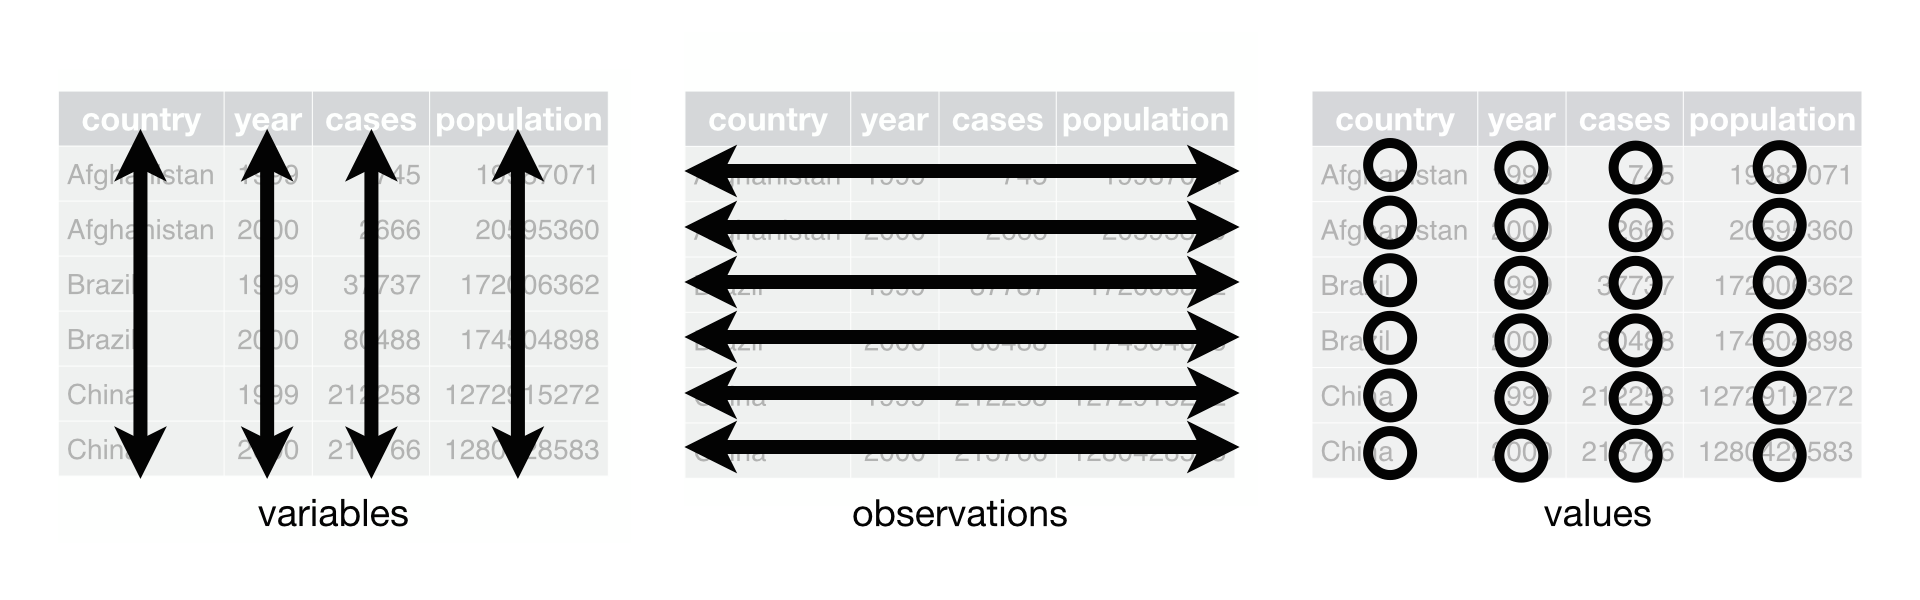
\includegraphics{Photos/tidy.png}
\caption{The components of a tidy dataset. \href{http://r4ds.had.co.nz/tidy-data.html}{Chapter 12} of R for Data Science}
\end{figure}

The transformation process from raw data to a tidy data format is often called \textbf{feature extraction} and is not a short or easy task. In this introductory course, we will typically work with data that are already in a tidy format.

What the row represents is often referred to as the \textbf{unit of analysis}. As data analysts, it is important for us to consider what to use as the unit of analysis. For example, this may come up when we have information on both individual presidents and their speeches. Do we want to understand matters at the individual level or the speech level? Answers to these questions will depend on the context and the research questions.

\hypertarget{data-context}{%
\section{Data Context}\label{data-context}}

For any data set, you should always ask yourself a few questions to provide vital \textbf{context} about that data set.

\begin{itemize}
\tightlist
\item
  \textbf{Who is in the data set?} What is the observational unit? How did they end up in the data set? Were they selected randomly or were they in a particular location a particular time?
\item
  \textbf{What is being measured or recorded on each unit?} What are the characteristics, features, or \emph{variables} that were collected?
\item
  \textbf{Where were they collected?} In one location? Multiple locations?
\item
  \textbf{When was the data collected?} One point in time? Over time? If data quality degrades over time (e.g.~lab specimens), we should be concerned.
\item
  \textbf{How were they collected?} What instruments and methods used for measurement? What questions were asked and how? Online survey? By phone? In person?
\item
  \textbf{Why were they collected?} For profit? For academic research? Are there conflicts of interest?
\item
  \textbf{Who collected this data?} An agency, a consortium of researchers, an individual researcher?
\end{itemize}

Thinking about this data context informs us how we analyze the data, what conclusions we can draw, and whether we can generalize our conclusions to a larger population.

Many of these data context questions also hint at general considerations for threats to data quality. Threats to data quality generally arise through \textbf{sampling}, \textbf{information bias}, and \textbf{study design.}

\hypertarget{sampling}{%
\section{Sampling}\label{sampling}}

When we study a phenomenon, we generally care about making a conclusion that applies to some \textbf{target population of interest} (e.g.~all likely voters in the U.S., all eligible voters in the U.S., college students in Minnesota, etc.). However, we cannot feasibly collect data on that entire population (this is called a \textbf{census} and is very expensive to complete) due to financial and time constraints, so we collect a \textbf{sample} of individuals. We want our sample to be \textbf{representative} of the target population in that we want our sample to resemble the target population in the characteristics we are studying.

\begin{reflect}
How is representativeness affected by our research question? Can a
sample be representative for one goal but not another?
\end{reflect}

When our method of selecting a sample is flawed, \textbf{sampling bias} can result, and our sample is unrepresentative of the target population. We need to be aware of how this tends to happen, and how can we avoid it.

It is first helpful to define the term \textbf{sampling frame}. A sampling frame is the complete list of individuals/units in the target population. For example, it could be a spreadsheet listing every college student that studies in Minnesota.

\hypertarget{sampling-bias}{%
\subsection{Sampling Bias}\label{sampling-bias}}

The following are common ways that sampling bias can arise, and they all share the feature that a sampling frame is \emph{NOT} used:

\begin{itemize}
\item
  \textbf{Convenience Sampling:} \emph{Individuals that make up a convenience sample are easy to contact or to reach (e.g.~you stand on a street corner and ask passerbys to answer a few questions). The people sampled will likely be systematically different than the target population.}
\item
  \textbf{Self-Selection and Volunteer Sampling:} \emph{Individuals that make up a sample self-select or volunteer to be in a sample (e.g.~product reviews on Amazon, individuals that call in to radio shows, blood donors, etc.). They are likely to be systematically different than the target population.}
\end{itemize}

One result of using these sampling techniques is that we can get \textbf{undercoverage} in the sample. This happens when some groups of the population are inadequately represented in the sample due to the sampling procedure. A famous example in United States history is the 1936 Literary Digest poll that completely mispredicted the presidential election. The magazine predicted a strong victory for Alfred Landon, but Franklin Delano Roosevelt ended up winning the election by a substantial margin. The survey relied on a convenience sample, drawn from telephone directories and car registration lists. In 1936, people who owned cars and telephones tended to be more affluent and leaned to the right politically (they favored Landon).

If we do not have a complete sampling frame, then we have no control over what units enter the sample because we do not even have a complete list of the units that \emph{could} be sampled. Imagine that our target population is like a pot of soup, these forms of sampling are similar to scooping only the bits of soup that float to the top of the pot without stirring.

\hypertarget{random-sampling}{%
\subsection{Random Sampling}\label{random-sampling}}

With a sampling frame, we can do better and hopefully avoid sampling bias by using randomization. In our soup metaphor, this amounts to mixing the soup thoroughly and dipping our spoon in random locations.

These strategies are called \textbf{probability sampling} strategies or, more colloquially, \textbf{random sampling} strategies. In probability sampling, each unit in the sampling frame has a known, nonzero probability of being selected, and the sampling is performed with some chance device (e.g.~coin flipping, random number generation).

Some probability sampling techniques include:

\textbf{Simple Random Sampling:} \emph{Each unit in the sampling frame has the same chance of being chosen and individuals are selected without replacement (once they have been chosen, they cannot be chosen again). With this strategy, every sample of a given size is equally likely to arise.}

\textbf{Stratified Sampling:} \emph{The units in the sampling frame are first divided into categories/strata (e.g.~age categories). Simple random sampling is then performed within each category/stratum. Why do this? Just by chance, simple random sampling might oversample young individuals. Stratifying by age first, then performing simple random sampling in these strata ensures a desired age distribution in the sample. With this strategy, you may be able to increase the precision of the estimates.}

\textbf{Cluster Sampling:} \emph{Sometimes a sampling frame is more readily available for clusters of units rather than the units themselves. For example, a sampling frame of all hospitals in Minnesota might be more readily available than a sampling frame of all Minnesota hospital patients in a given time frame. In cluster sampling, the initial clusters are sampled with a probability sampling method (like simple random sampling or stratified sampling). All units in the sampled clusters may be chosen, or if sampling frames can be obtained for the sampled clusters, probability sampling is performed within the cluster. This strategy should only be used when a full sampling frame is unavailable or it is economically justified as this procedure generally provides less precision than the other two strategies.}

\hypertarget{nonresponse-bias}{%
\subsection{Nonresponse bias}\label{nonresponse-bias}}

Even with a random sampling method, our sample can still be unrepresentative if units in our sample do not choose to participate after they are selected. For example, if the communication method is via e-mail, individuals who do not read our e-mail may be nonresponders. If those individuals who don't participate are systematically different than those that do, this type of nonresponse bias is called \textbf{unit nonresponse bias}.

Let's say that an individual opens up our e-mail survey. They may answer the first few questions but grow weary and skip the last questions. If those individuals who answer some but don't answer other questions are systematically different than those that do in their responses, this type of nonresponse bias is called \textbf{item nonresponse bias}.

\hypertarget{information-bias}{%
\section{Information bias}\label{information-bias}}

Lastly, separate from sampling, bias can arise in how we record or measure observations. Some of these biases are types of cognitive biases that and others are statistical biases. Here are a few types of information biases that can occur:

\begin{itemize}
\tightlist
\item
  \textbf{Response bias/Self-report bias/Social desirability bias:} \emph{Bias occurs when the recorded response does not accurately represent the true value for the individual due to wording of the question, ordering of the questions, format of response, or to increase social desirability. Most people like to present themselves in a favorable light, so they will be reluctant to admit to unsavory attitudes or characteristics (e.g.~weight, income, alcohol consumption, mental illness) or illegal activities in a survey, particularly if the survey is completed in an interview setting and/or the results are not confidential. Additionally, this could arise if the possible responses do not allow for accurate reporting (e.g.~\href{https://www.hrc.org/resources/collecting-transgender-inclusive-gender-data-in-workplace-and-other-surveys}{gender identity}, \href{https://www.pewsocialtrends.org/interactives/multiracial-timeline/}{race}).}
\item
  \textbf{Recall bias:} \emph{People often unintentionally make mistakes in remembering details about the past. If the study design is retrospective in that it requires units to rely on their memory, we may get bias in the information collected.}
\item
  \textbf{Measurement error:} \emph{Technologies that measure variables of interest may not always be accurate and human calibration of those instruments may be off as well.}
\end{itemize}

There are many other forms of bias, many of which are studied by cognitive and social pscyhologists. When designing questionnaires and surveys, it is important to keep these in mind. A researcher must first decide what specific information they want to collect and then figure out the best way to accurately collect that.

\hypertarget{study-design}{%
\section{Study Design}\label{study-design}}

Once we have a sample selected, data can be collected in one of two general study designs:

\begin{enumerate}
\def\labelenumi{\arabic{enumi}.}
\item
  \textbf{Observational Study:} \emph{Data is collected in such a way such that the researcher \textbf{does not} manipulate or intervene in the characteristics of the individuals. Researchers observe or record characteristics of the sample through direct measurement or through a questionnaire or survey.}
\item
  \textbf{Experiment:} \emph{Data is collected in such a way such that the researcher \textbf{does} manipulate or intervene in characteristics of the individuals by randomly assigning individuals to treatment or control groups. Researchers then record characteristics of the individuals in the sample within the treatment and control groups.}
\end{enumerate}

The main reason for doing an experiment is to estimate a relationship between a treatment and a response.

For example, imagine that we want to know if taking a daily multivitamin reduces systolic blood pressure. If we performed an observational study, we would select a sample (hopefully a representative one) from a population of interest and then ask whether an individual takes a daily multivitamin and then measure their blood pressure. \emph{Would this data provide enough evidence to conclude that vitamin use causes a reduction in blood pressure?}

Individuals that take daily multivitamins may be more health-conscious, eating more fruits and vegetables and exercising more, which may be related to blood pressure. The diet and exercise would be acting as \textbf{confounding variables}, making it impossible to say for certain if vitamin use has a direct impact on blood pressure.

\textbf{Confounding Variables:} \emph{A third variable that is a common cause for the ``treatment'' (e.g.~multivitamin) and the ``response'' (e.g.~blood pressure). In this case, a healthy lifestyle could be a variable that confounds the relationship between multivitamin use and blood pressure.}

\begin{Shaded}
\begin{Highlighting}[]
\KeywordTok{confounder_triangle}\NormalTok{(}\DataTypeTok{y=} \StringTok{"Blood}\CharTok{\textbackslash{}n}\StringTok{ Pressure"}\NormalTok{, }
                  \DataTypeTok{z =} \StringTok{"Healthy}\CharTok{\textbackslash{}n}\StringTok{ Lifestyle"}\NormalTok{,}
                  \DataTypeTok{x=} \StringTok{"Multivitamin}\CharTok{\textbackslash{}n}\StringTok{ Use"}\NormalTok{) }\OperatorTok
\KeywordTok{ggdag}\NormalTok{( }\DataTypeTok{text =} \OtherTok{FALSE}\NormalTok{, }\DataTypeTok{use_labels =} \StringTok{"label"}\NormalTok{) }\OperatorTok{+}
\StringTok{  }\KeywordTok{theme_dag_blank}\NormalTok{()}
\end{Highlighting}
\end{Shaded}

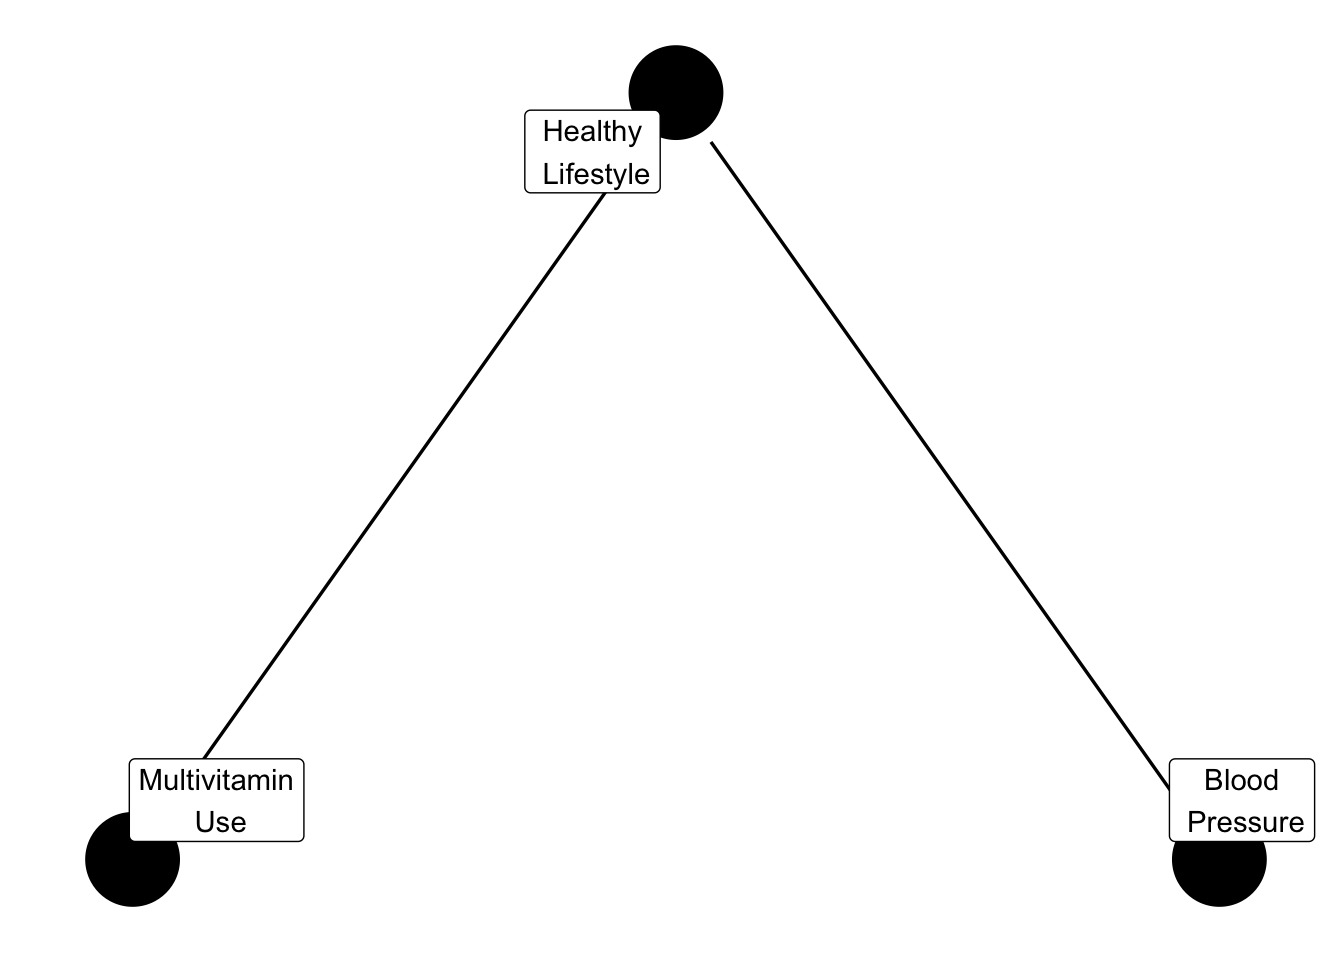
\includegraphics{01-data_files/figure-latex/unnamed-chunk-3-1.pdf}

\begin{reflect}
For example, say we note that on days with higher ice cream sales, there
are typically a higher number of pool drownings. What variable could be
confounding the relationship between ice cream sales and pool drownings?
\end{reflect}

In an experiment, we ``manipulate'' the characteristics for an individual by randomly assigning them to a treatment group. This random assignment is intended to break the relationship between any common causes and the treatment so as to try to reduce the impact of confounding. It is impossible to entirely remove the possibility of confounding, but the random assignment to a treatment helps. (Note: things can get complicated if individuals don't comply with the treatment such as take the multivitamin every single day\ldots)

\hypertarget{cause-and-effect}{%
\section{Cause and Effect}\label{cause-and-effect}}

Causal inference is the process of making a conclusion about direct cause and effect between a ``treatment'' and a ``response''. It is difficult to make causal statements based on data from an observational study due to the possible presence of confounding variables.

There is a whole area of statistics dedicated to methods that attempt to overcome the potential confounding. We'll talk more about causal inference in (Section \ref{dag}).

\hypertarget{ethical-considerations}{%
\section{Ethical Considerations}\label{ethical-considerations}}

Ethics play a very important role in study design and data collection procedures, especially when humans and animals are the observational units. In the United States, the \href{https://www.hhs.gov/ohrp/regulations-and-policy/belmont-report/index.html}{Belmont Report} is the main federal document that provides the ``Ethical Principles and Guidelines for the Protection of Human Subjects of Research''. The three fundamental ethical principles for using any human subjects for research are:

\begin{enumerate}
\def\labelenumi{\arabic{enumi}.}
\item
  \textbf{Respect for persons}: This principle is about protecting the autonomy of all people and treating them with courtesy and respect and allowing for informed consent. Researchers must be truthful and conduct no deception;
\item
  \textbf{Beneficence}: This principle is the philosophy of ``do no harm'' while maximizing benefits for the research project and minimizing risks to the research subjects; and
\item
  \textbf{Justice}: This principle is about ensuring reasonable, non-exploitative, and well-considered procedures are administered fairly --- the fair distribution of costs and benefits to potential research participants --- and equally.
\end{enumerate}

For a brief, limited history of ethical regulation in human research, see \url{https://www.ncbi.nlm.nih.gov/pmc/articles/PMC3593469/}. A few key moments in international history are

\begin{itemize}
\tightlist
\item
  \href{https://www.nejm.org/doi/full/10.1056/NEJM199711133372006}{Nuremberg Code} (1948) in response to medical experiments in Germany performed without consent
\item
  \href{https://www.wma.net/what-we-do/medical-ethics/}{Declaration of Helskinki} (originated in 1964 and frequently revised) established by World Medical Association.
\item
  The Belmont Report written in response to the Tuskegee Syphilis Study (1932 - 1972).
\item
  \href{https://www.hhs.gov/ohrp/regulations-and-policy/regulations/common-rule/index.html}{Common Rule} (1981) is regulatory policy which all U.S. government-funded research and nearly all U.S. academic institutions must abide.
\end{itemize}

Macalester College has an Institutional Review Board (IRB) that oversees research at Macalester that includes human participants (see: \url{https://www.macalester.edu/irb/}).

Throughout this class, we are going to stop and think about the ethical considerations of the many parts of statistical practice, ranging from data collection to model prediction.

\textbf{Ethics} are the norms or standards for conduct that distinguish between right and wrong. In particular, we are going to consider the ethics of

\begin{itemize}
\tightlist
\item
  How the data are collected
\item
  Random assignment to treatments
\item
  Data storage
\item
  Data privacy
\item
  Data use
\item
  Choice of sample data used for predictive modeling
\item
  Use of predictive modeling
\end{itemize}

We are going to pay extra attention to negative consequences of the above that may disproportionately impact marginalized groups of people.

Throughout the semester, you will be asked to think about answers to the question: ``What are the ethical considerations for this data set/analysis?'' Like in other disciplines, the choices we make will be biased by our life experiences. Throughout this class, let us be mindful in increasing our awareness of the real consequences caused by choices we make in Statistics.

\hypertarget{chapter-1-major-takeaways}{%
\section{Chapter 1 Major Takeaways}\label{chapter-1-major-takeaways}}

\begin{enumerate}
\def\labelenumi{\arabic{enumi}.}
\item
  Any observed data is a sample of a larger population or phenomenon. But you need to consider which population. Is it the population of interest to you? If not, then why?
\item
  Sampling strategies impact what type of generalizations we can make about a population. Bias occurs when there are systematic differences between observed sample data and the true population of interest due to the sampling process.
\item
  The data we collect many not accurately reflect the truth due to information biases caused by the data collection mechanism (instrument or survey).
\item
  Study design impacts what type of conclusions we can make. Confounding variables prevent us from easily making cause and effect conclusions.
\item
  We need to be aware of the real and ethical consequences of our choices when working with data and building statistical models.
\end{enumerate}

\hypertarget{visualizing-data}{%
\chapter{Visualizing Data}\label{visualizing-data}}

The first step in any data analysis is to visually explore your data.

There is a saying that ``a picture is worth a 1000 words.'' In making visualizations, our goal is to quickly and easily get a better understanding of the variability, structure, and relationships that exist in the data.

Here we will cover the standard appropriate graphics for univariate variation and bivariate relationships. We will also cover techniques for multivariate relationships (3 or more variables). The choice of the graphic depends on the type(s) of variable(s): quantitative or categorical. Thus, the first step in creating a graphic is to think about the variables that you are interested in visualizing and determining whether they are quantitative or categorical.

For each type of variable, we use a real dataset to illustrate the visualizations.

\hypertarget{good-visualization-principles}{%
\section{Good Visualization Principles}\label{good-visualization-principles}}

Before we discuss the standard graphics, let's lay out the basic design principles for good data visualizations.

\begin{enumerate}
\def\labelenumi{\arabic{enumi}.}
\item
  \textbf{Show the data:} This may be self-explanatory, but make sure that the data is the focus and driver of the visualization.
\item
  \textbf{Avoid distorting the data:} Avoid 3D charts as the added dimension distorts the comparison. The area in a graph should equal the magnitude of the data it is representing.
\item
  \textbf{Simplify:} In 1983, Edward Tufte said that ``A large share of ink on a graphic should present data-information, the ink changing as the data change. Data-ink is the non-erasable core of a graphic, the non-redundant ink arranged in response to variation in the numbers represented.'' Remove any unnecessary ``ink'' that does not assist in the presentation of the data. Remove distractions.
\item
  \textbf{Facilitate comparisons:} In order to explain variation, we want the graphics to facilitate comparisons between groups. The design should make it easier to compare between groups rather than harder.
\item
  \textbf{Use contrast:} Humans have developed to seek out visual contrast. When choosing colors and annotation, strive for more contrast in luminance (white to dark) to make it easier for everyone to visually perceive.
\item
  \textbf{Use color appropriately:} Think about your audience. A small proportion of the population is color-blind; try printing it in grayscale to see if the color palette is still effective. Also, every culture has different associations with colors; ask others for feedback on color choices. Neuroscience research has shown that humans are more sensitive to red and yellow, so those are good colors to use for highlighting key points.
\item
  \textbf{Annotate appropriately:} Informative text is crucial for providing data context. Make sure to use informative axis labels and titles. It may be worth adding text to explain extreme outliers.
\end{enumerate}

For examples of good data visualizations in the news and discussion around them, check out the New York Times column \href{https://www.nytimes.com/column/whats-going-on-in-this-graph}{``What's Going on in This Graph?''}.

\hypertarget{brief-intro-to-r}{%
\section{Brief Intro to R}\label{brief-intro-to-r}}

Throughout this class, we use R and RStudio to visualize, analyze, and model real data. To straighten out which is which: \href{https://cran.r-project.org/}{R} is the name of the language itself (syntax, words, etc.) and \href{https://www.rstudio.com/}{RStudio} is a convenient software interface that you'll interact with on the computer.

While you'll be learning about and using R throughout the course, this is not a course on R. Our focus will be on data and statistical modelling. We will be using R and RStudio as tools to help us get information from data.

\hypertarget{basic-syntax}{%
\subsection{Basic Syntax}\label{basic-syntax}}

For this class, we will have data that we want to pass to a function that performs a particular operation (does something cool) on our data. Thus, we'll pass \textbf{inputs} as arguments to a \textbf{function}:

\begin{verbatim}
FunctionName(argument1 = a1, argument2 = a2,..., argumentk = ak)
\end{verbatim}

Note the \texttt{FunctionName} and the use of parantheses. Inside the parantheses, the argument name (\texttt{argument1}) goes first and the value you are passing as an input is after = (\texttt{a1}).

We may want to save the \textbf{output} of the function by assigning it a name using the assignment operator, \texttt{\textless{}-}:

\begin{verbatim}
OutputName <- FunctionName(argument1 = a1, argument2 = a2,..., argumentk = ak)
\end{verbatim}

R allows us to be lazy and not include the argument name as long as we provide the input in the correct order:

\begin{verbatim}
OutputName <- FunctionName(a1, a2,..., ak)
\end{verbatim}

We can also \textbf{nest} functions by first performing one operation and then passing that as an input into another function. In the code below, \texttt{Function1()} would first run with the input \texttt{data} and create some output that is then passed as the first input in \texttt{Function2()}. So R evaluates functions from the inside-out.

\begin{verbatim}
Function2(Function1(data))
\end{verbatim}

As we go through real examples below, notice the names of the functions that we use. The name comes right before \texttt{(} and the inputs we pass in right after \texttt{(}.

Additionally, we are going to use a shortcut that makes our code more readable. It is called a \textbf{pipe} and looks like \texttt{\%\textgreater{}\%}. What this does is pass the output on its left as the first argument to the function on the right. The following two sections of code do exactly the same thing but the second is easier to read. For this code, we take data and summarize the variable height and then take the mean of the heights.

\begin{verbatim}
summarize(data, mean(height))

data %>%
  summarize(mean(height))
\end{verbatim}

There is so much more we could say about functions in R, but we will stop here for now.

With this in mind, we'll point to external references if you'd like to go deeper in your understanding of R as a programming language throughout this class.

To get a broad sense of R, you can work through R primers (\url{https://rstudio.cloud/learn/primers}) in RStudio Cloud in addition to any coursework and use the R cheatsheets available online (\url{https://rstudio.cloud/learn/cheat-sheets}).

\hypertarget{anatomy-of-a-ggplot-command}{%
\section{Anatomy of a ggplot command}\label{anatomy-of-a-ggplot-command}}

To learn more about visualizing data with the ggplot2 R package, see \href{https://r4ds.had.co.nz/data-visualisation.html}{Hadley Wickham's textbook}.

In this course, we'll largely construct visualizations using the \texttt{ggplot()} function from the \texttt{ggplot2} R package. NOTE: \texttt{gg} is short for ``grammar of graphics''. Plots constructed from the \texttt{ggplot()} function are constructed in layers, and the syntax used to create plots is meant to reflect this layered construction. As you read through the rest of this chapter, pay attention to how the syntax generally follows this structure:

\begin{Shaded}
\begin{Highlighting}[]
\NormalTok{data }\OperatorTok
\StringTok{    }\KeywordTok{ggplot}\NormalTok{(}\KeywordTok{aes}\NormalTok{(}\DataTypeTok{x =}\NormalTok{ X_AXIS_VARIABLE, }\DataTypeTok{y =}\NormalTok{ Y_AXIS_VARIABLE)) }\OperatorTok{+}
\StringTok{    }\NormalTok{VISUAL_LAYER1 }\OperatorTok{+}
\StringTok{    }\NormalTok{VISUAL_LAYER2 }\OperatorTok{+}
\StringTok{    }\NormalTok{VISUAL_LAYER3 }\OperatorTok{+}\StringTok{ }\NormalTok{...}
\end{Highlighting}
\end{Shaded}

We pass the aesthetic mapping from the data set to the plot with \texttt{aes()}. The visual layers are features such as points, lines, and panels. We'll introduce these soon. The \texttt{+}'s allow us to add layers to build up a plot (note this is not the pipe!).

\begin{reflect}
What are the function names in the example above? There are only two as
it is written right now.
\end{reflect}

\hypertarget{one-categorical-variable}{%
\section{One Categorical Variable}\label{one-categorical-variable}}

First, we consider survey data of the electoral registrar in Whickham in the UK (Source: Appleton et al 1996). A survey was conducted in 1972-1974 to study heart disease and thyroid disease and a few baseline characteristics were collected: age and smoking status. 20 years later, a follow-up was done to check on mortality status (alive/dead).

Let's first consider the age distribution of this sample. Age, depending on how it is measured, could act as a quantitative variable or categorical variable. In this case, age is recorded as a quantitative variable because it is recorded to the nearest year. But, for illustrative purposes, let's create a categorical variable by separating age into intervals.

\textbf{Distribution:} \emph{the way something is spread out (the way in which values vary).}

\begin{Shaded}
\begin{Highlighting}[]
\CommentTok{# Note: anything to the right of a hashtag is a comment and is not evaluated as R code}

\KeywordTok{library}\NormalTok{(dplyr) }\CommentTok{# Load the dplyr package}
\KeywordTok{library}\NormalTok{(ggplot2) }\CommentTok{# Load the ggplot2 package}
\KeywordTok{data}\NormalTok{(Whickham) }\CommentTok{# Load the data set from Whickham R package}

\NormalTok{Whickham <-}\StringTok{ }\NormalTok{Whickham }\OperatorTok
\StringTok{    }\KeywordTok{mutate}\NormalTok{(}\DataTypeTok{ageCat =} \KeywordTok{cut}\NormalTok{(age, }\DecValTok{4}\NormalTok{)) }\CommentTok{# Create a new categorical variable with 4 categories based on age (equal length of age intervals)}

\KeywordTok{head}\NormalTok{(Whickham)}
\end{Highlighting}
\end{Shaded}

\begin{verbatim}
##   outcome smoker age      ageCat
## 1   Alive    Yes  23 (17.9,34.5]
## 2   Alive    Yes  18 (17.9,34.5]
## 3    Dead    Yes  71 (67.5,84.1]
## 4   Alive     No  67   (51,67.5]
## 5   Alive     No  64   (51,67.5]
## 6   Alive    Yes  38   (34.5,51]
\end{verbatim}

\begin{reflect}
What do you lose when you convert a quantitative variable to a
categorical variable? What do you gain?
\end{reflect}

\hypertarget{bar-plot}{%
\subsection{Bar Plot}\label{bar-plot}}

One of the best ways to show the distribution of one categorical variable is with a bar plot. For a bar plot,

\begin{itemize}
\tightlist
\item
  The \textbf{height of the bars} is the only part that encodes the data (width is meaningless).
\item
  The height can either represent the \textbf{frequency} (count of units) or the \textbf{relative frequency} (proportion of units).
\end{itemize}

\begin{Shaded}
\begin{Highlighting}[]
\CommentTok{## Numerical summary (frequency and relative frequency)}
\NormalTok{Whickham }\OperatorTok
\StringTok{    }\KeywordTok{count}\NormalTok{(ageCat) }\OperatorTok
\StringTok{    }\KeywordTok{mutate}\NormalTok{(}\DataTypeTok{relfreq =}\NormalTok{ n }\OperatorTok{/}\StringTok{ }\KeywordTok{sum}\NormalTok{(n)) }
\end{Highlighting}
\end{Shaded}

\begin{verbatim}
##        ageCat   n   relfreq
## 1 (17.9,34.5] 408 0.3105023
## 2   (34.5,51] 367 0.2792998
## 3   (51,67.5] 347 0.2640791
## 4 (67.5,84.1] 192 0.1461187
\end{verbatim}

\begin{Shaded}
\begin{Highlighting}[]
\CommentTok{## Graphical summary (bar plot)}
\NormalTok{Whickham }\OperatorTok
\StringTok{    }\KeywordTok{ggplot}\NormalTok{(}\KeywordTok{aes}\NormalTok{(}\DataTypeTok{x =}\NormalTok{ ageCat)) }\OperatorTok{+}\StringTok{ }
\StringTok{    }\KeywordTok{geom_bar}\NormalTok{(}\DataTypeTok{fill=}\StringTok{"steelblue"}\NormalTok{) }\OperatorTok{+}\StringTok{ }
\StringTok{    }\KeywordTok{xlab}\NormalTok{(}\StringTok{'Age Categories in Years'}\NormalTok{) }\OperatorTok{+}\StringTok{ }
\StringTok{    }\KeywordTok{ylab}\NormalTok{(}\StringTok{'Counts'}\NormalTok{) }\OperatorTok{+}\StringTok{ }
\StringTok{    }\KeywordTok{theme_minimal}\NormalTok{()}
\end{Highlighting}
\end{Shaded}

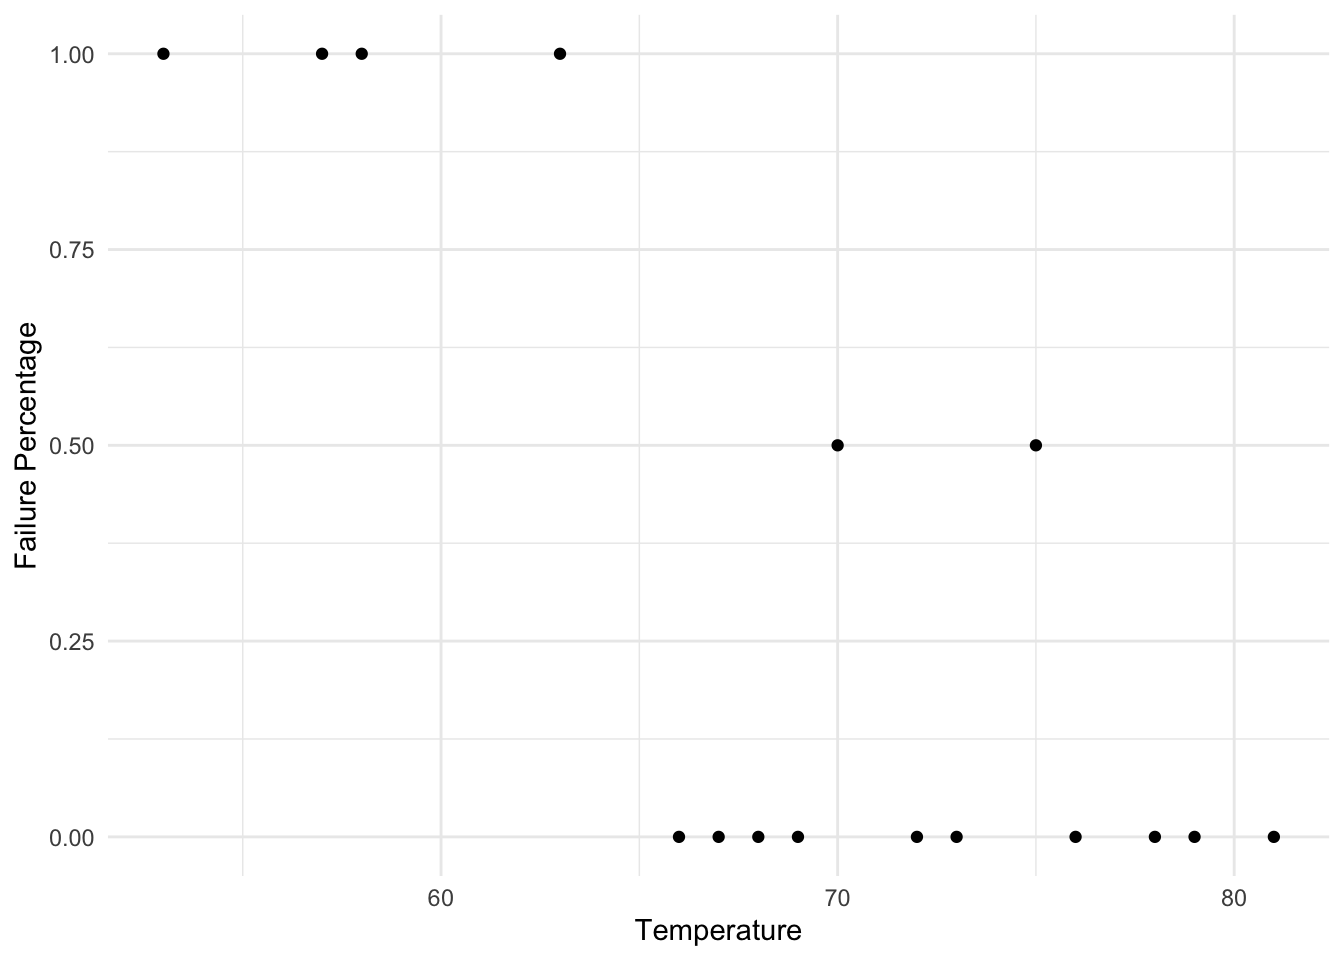
\includegraphics{02-visualization_files/figure-latex/unnamed-chunk-5-1.pdf}

\begin{reflect}
What do you notice? What do you wonder?
\end{reflect}

\hypertarget{pie-chart}{%
\subsection{Pie Chart}\label{pie-chart}}

Pie charts are only useful if you have 2 to 3 possible categories and you want to show relative group sizes.

This is the best use for a pie chart:

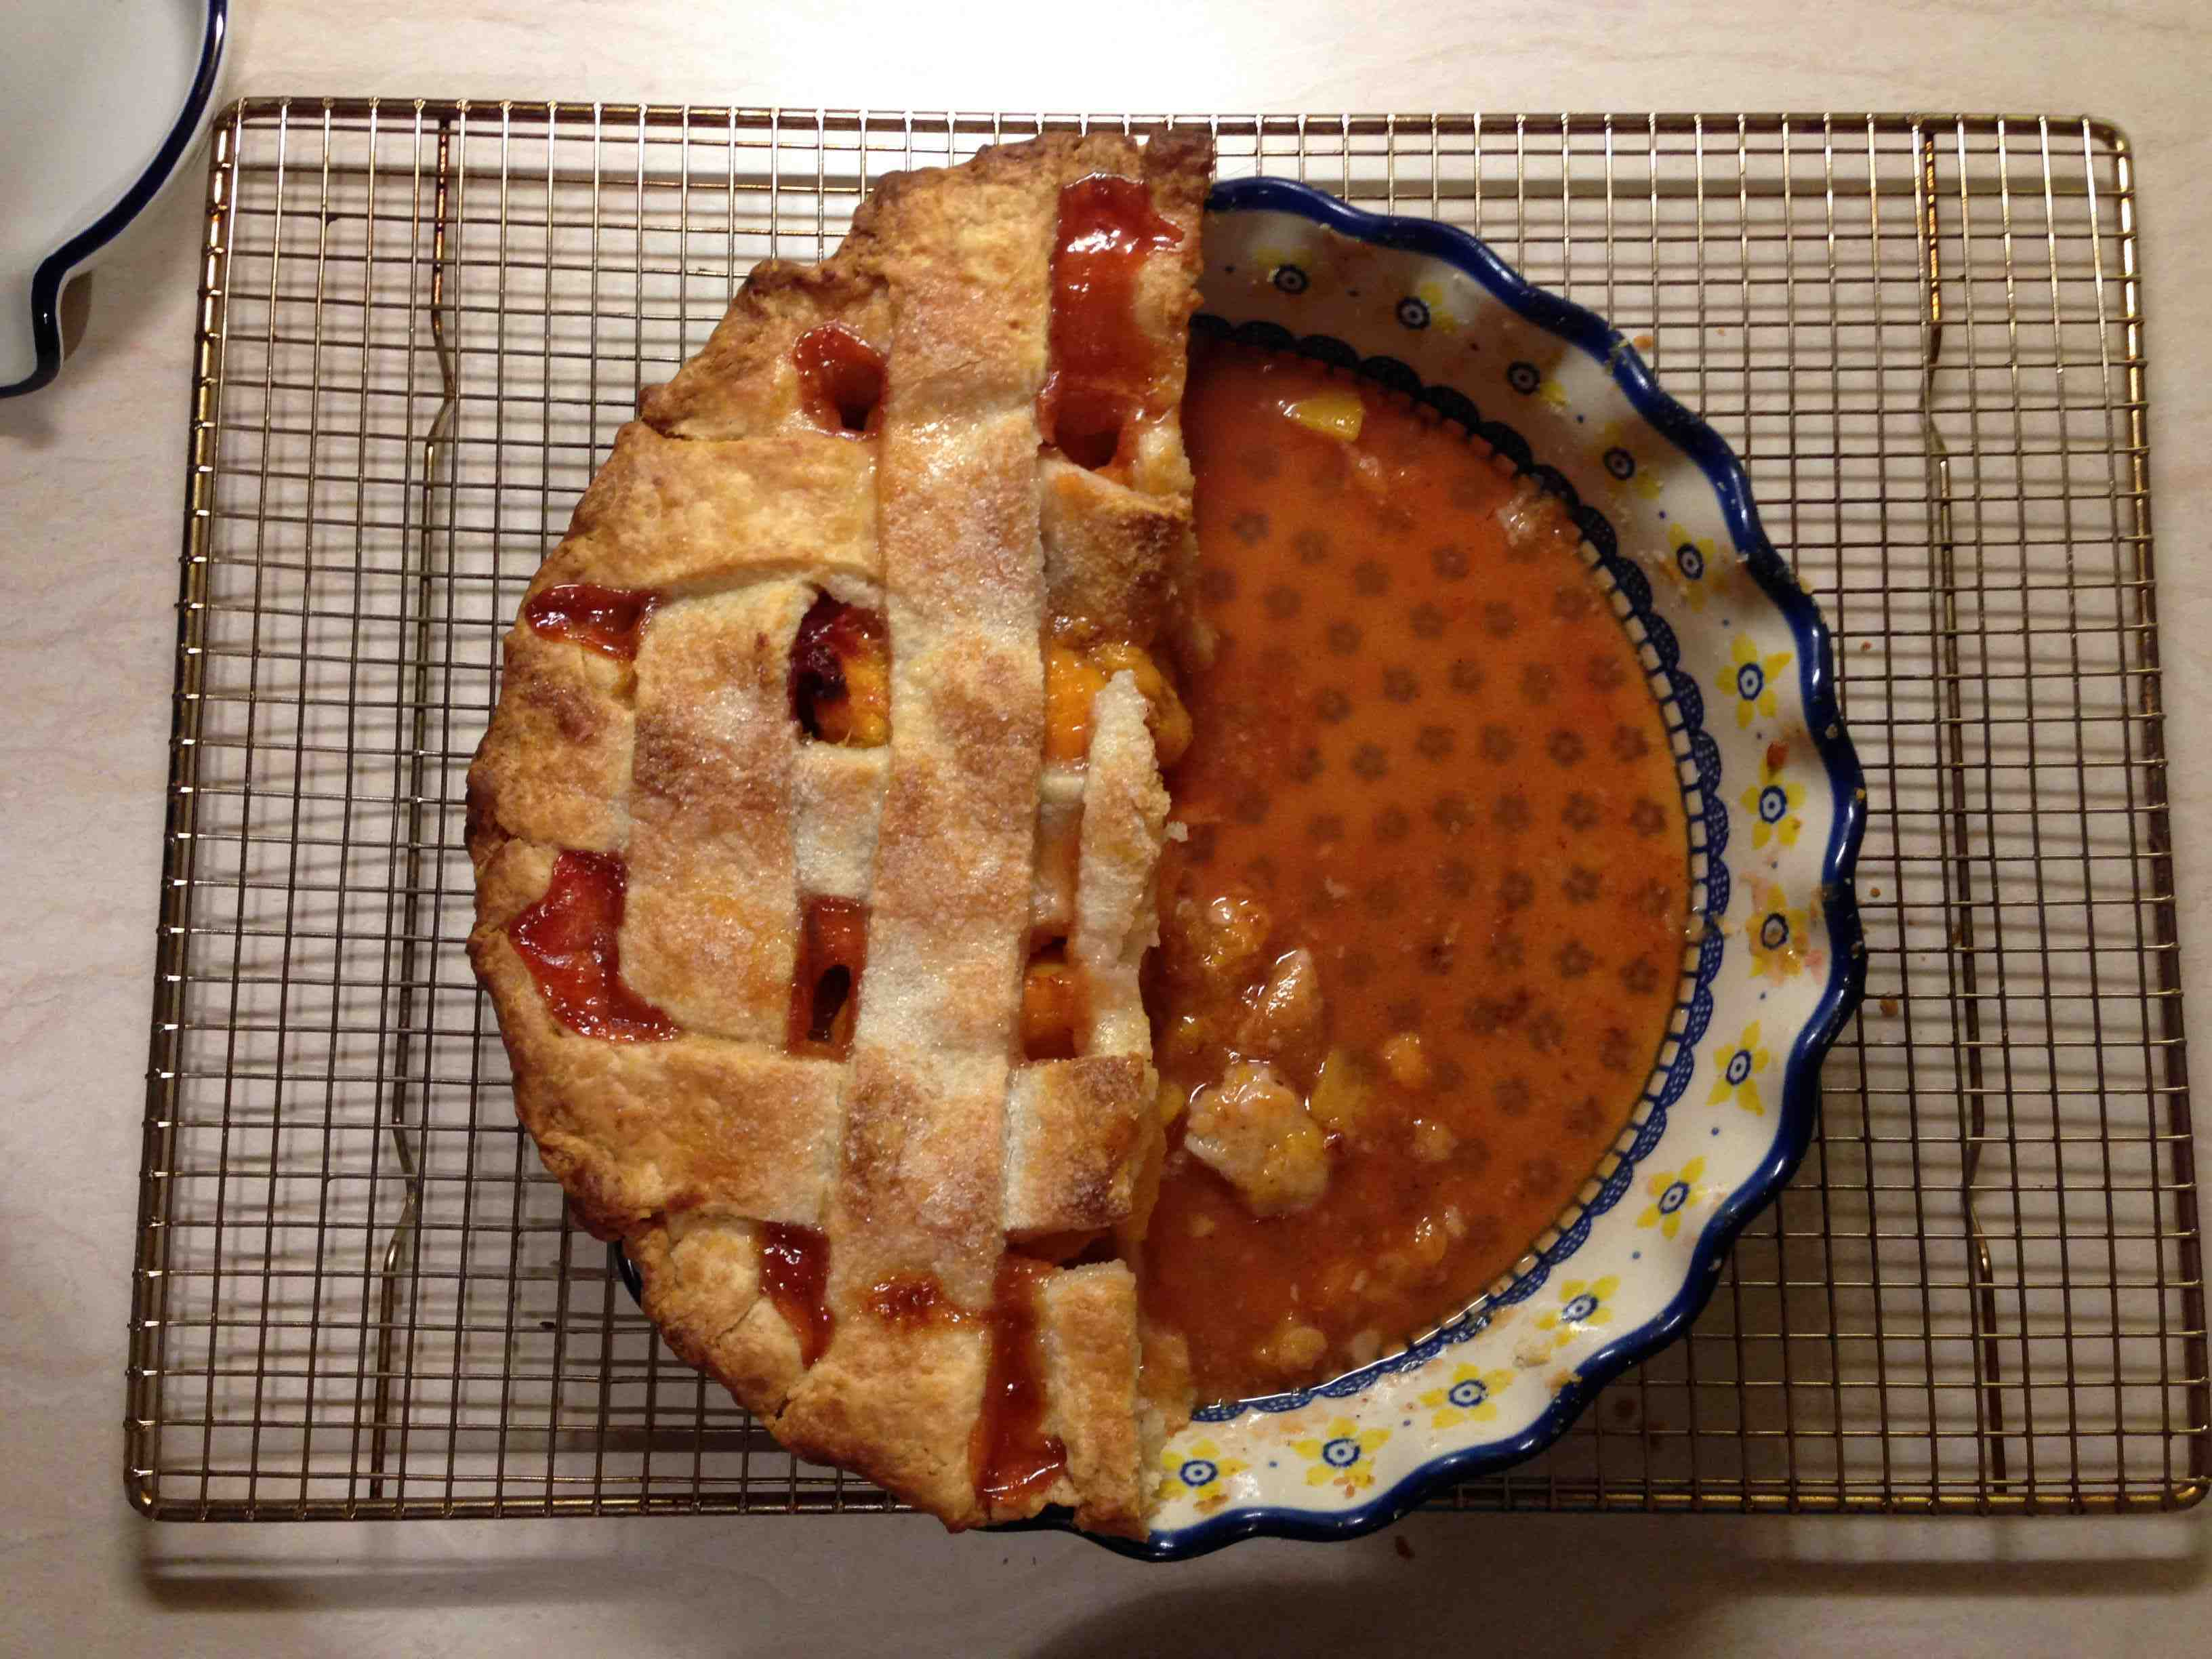
\includegraphics[width=.25\textwidth]{Photos/pie}

We are intentionally not showing you how to make a pie chart because a bar chart is a better choice.

Here is a good summary of why many people strongly dislike pie charts: \url{http://www.businessinsider.com/pie-charts-are-the-worst-2013-6}. Keep in mind Visualization Principle \#4: Facilitate Comparisons. We are much better at comparing heights of bars than areas of slices of a pie chart.

\hypertarget{two-categorical-variables}{%
\section{Two Categorical Variables}\label{two-categorical-variables}}

Now, let's consider two other variables in the same Whickham data set. What is the relationship between the 20-year mortality outcome and smoking status at the beginning of the study?

\hypertarget{side-by-side-bar-plot}{%
\subsection{Side by Side Bar Plot}\label{side-by-side-bar-plot}}

There are a few options for visualizing the relationship between two categorical variables. One option is to use a bar plot and add bars for different categories next to each other, called a \textbf{side-by-side bar plot}. For these plots,

\begin{itemize}
\tightlist
\item
  The \textbf{height of the bars} shows the frequency of the categories within subsets.
\end{itemize}

\begin{Shaded}
\begin{Highlighting}[]
\CommentTok{## Numerical summary (frequency and overall relative frequency)}
\NormalTok{Whickham }\OperatorTok
\StringTok{  }\KeywordTok{count}\NormalTok{(outcome, smoker) }\OperatorTok
\StringTok{  }\KeywordTok{mutate}\NormalTok{(}\DataTypeTok{relfreq =}\NormalTok{ n }\OperatorTok{/}\StringTok{ }\KeywordTok{sum}\NormalTok{(n))}
\end{Highlighting}
\end{Shaded}

\begin{verbatim}
##   outcome smoker   n   relfreq
## 1   Alive     No 502 0.3820396
## 2   Alive    Yes 443 0.3371385
## 3    Dead     No 230 0.1750381
## 4    Dead    Yes 139 0.1057839
\end{verbatim}

\begin{Shaded}
\begin{Highlighting}[]
\CommentTok{## Graphical summary (side-by-side bar plot)}
\NormalTok{Whickham }\OperatorTok
\StringTok{  }\KeywordTok{ggplot}\NormalTok{(}\KeywordTok{aes}\NormalTok{(}\DataTypeTok{x =}\NormalTok{ smoker, }\DataTypeTok{fill =}\NormalTok{ outcome)) }\OperatorTok{+}\StringTok{ }
\StringTok{  }\KeywordTok{geom_bar}\NormalTok{(}\DataTypeTok{position =} \KeywordTok{position_dodge}\NormalTok{()) }\OperatorTok{+}\StringTok{ }
\StringTok{  }\KeywordTok{xlab}\NormalTok{(}\StringTok{'Smoker Status'}\NormalTok{) }\OperatorTok{+}\StringTok{ }
\StringTok{  }\KeywordTok{ylab}\NormalTok{(}\StringTok{'Counts'}\NormalTok{) }\OperatorTok{+}\StringTok{ }
\StringTok{  }\KeywordTok{scale_fill_manual}\NormalTok{(}\StringTok{'20 Year Mortality'}\NormalTok{, }\DataTypeTok{values =} \KeywordTok{c}\NormalTok{(}\StringTok{"steelblue"}\NormalTok{, }\StringTok{"lightblue"}\NormalTok{)) }\OperatorTok{+}\StringTok{ }
\StringTok{  }\KeywordTok{theme_minimal}\NormalTok{()}
\end{Highlighting}
\end{Shaded}

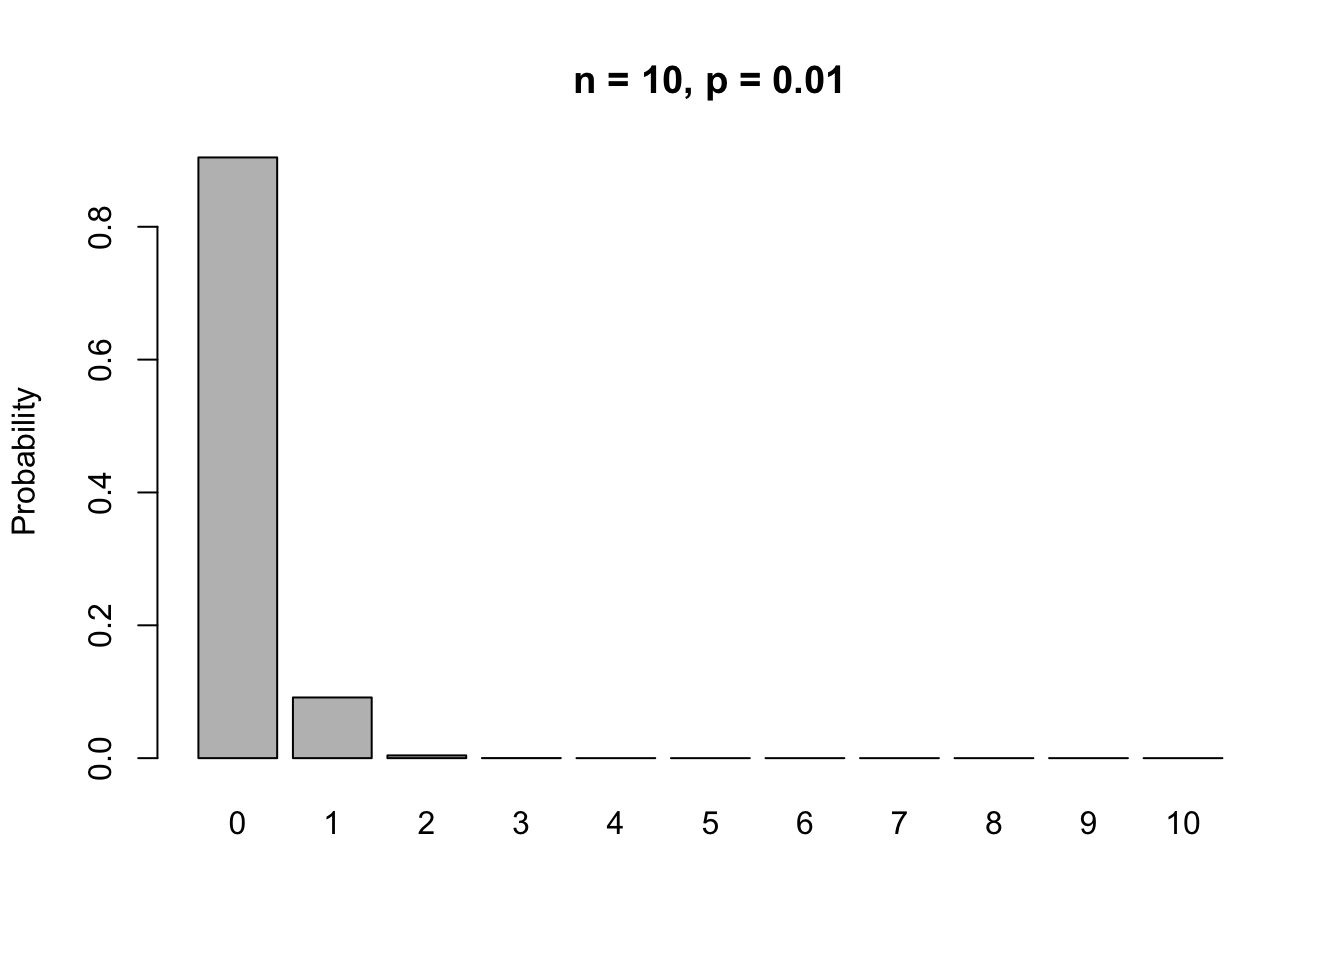
\includegraphics{02-visualization_files/figure-latex/unnamed-chunk-8-1.pdf}

\begin{reflect}
What additional information do you gain by considering smoking status?
\end{reflect}

\hypertarget{stacked-bar-plot}{%
\subsection{Stacked Bar Plot}\label{stacked-bar-plot}}

Another way to show the same data is by stacking the bars on top of each other with a category. For a \textbf{stacked bar plot},

\begin{itemize}
\tightlist
\item
  The \textbf{height} of the entire bar shows the \textbf{marginal distribution} (frequency of the X variable, ignoring the other variable).
\item
  The \textbf{relative heights} show \textbf{conditional distributions} (frequencies within subsets), but it is hard to compare distributions between bars because the overall heights differ.
\item
  The \textbf{widths} of the bars have no meaning.
\end{itemize}

\begin{Shaded}
\begin{Highlighting}[]
\CommentTok{## Numerical summary (conditional distribution - conditioning on outcome)}
\NormalTok{Whickham }\OperatorTok
\StringTok{    }\KeywordTok{count}\NormalTok{(outcome, smoker) }\OperatorTok
\StringTok{    }\KeywordTok{group_by}\NormalTok{(outcome) }\OperatorTok
\StringTok{    }\KeywordTok{mutate}\NormalTok{(}\DataTypeTok{relfreq =}\NormalTok{ n }\OperatorTok{/}\StringTok{ }\KeywordTok{sum}\NormalTok{(n)) }
\end{Highlighting}
\end{Shaded}

\begin{verbatim}
## # A tibble: 4 x 4
## # Groups:   outcome [2]
##   outcome smoker     n relfreq
##   <fct>   <fct>  <int>   <dbl>
## 1 Alive   No       502   0.531
## 2 Alive   Yes      443   0.469
## 3 Dead    No       230   0.623
## 4 Dead    Yes      139   0.377
\end{verbatim}

\begin{Shaded}
\begin{Highlighting}[]
\CommentTok{## Numerical summary (conditional distribution - conditioning on smoker)}
\NormalTok{Whickham }\OperatorTok
\StringTok{    }\KeywordTok{count}\NormalTok{(outcome, smoker) }\OperatorTok
\StringTok{    }\KeywordTok{group_by}\NormalTok{(smoker) }\OperatorTok
\StringTok{    }\KeywordTok{mutate}\NormalTok{(}\DataTypeTok{relfreq =}\NormalTok{ n }\OperatorTok{/}\StringTok{ }\KeywordTok{sum}\NormalTok{(n)) }
\end{Highlighting}
\end{Shaded}

\begin{verbatim}
## # A tibble: 4 x 4
## # Groups:   smoker [2]
##   outcome smoker     n relfreq
##   <fct>   <fct>  <int>   <dbl>
## 1 Alive   No       502   0.686
## 2 Alive   Yes      443   0.761
## 3 Dead    No       230   0.314
## 4 Dead    Yes      139   0.239
\end{verbatim}

\begin{Shaded}
\begin{Highlighting}[]
\CommentTok{## Graphical summary (stacked bar plot)}
\NormalTok{Whickham }\OperatorTok
\StringTok{    }\KeywordTok{ggplot}\NormalTok{(}\KeywordTok{aes}\NormalTok{(}\DataTypeTok{x =}\NormalTok{ smoker, }\DataTypeTok{fill =}\NormalTok{ outcome)) }\OperatorTok{+}\StringTok{ }
\StringTok{    }\KeywordTok{geom_bar}\NormalTok{() }\OperatorTok{+}\StringTok{ }
\StringTok{    }\KeywordTok{xlab}\NormalTok{(}\StringTok{'Smoker Status'}\NormalTok{) }\OperatorTok{+}\StringTok{ }
\StringTok{    }\KeywordTok{ylab}\NormalTok{(}\StringTok{'Counts'}\NormalTok{) }\OperatorTok{+}\StringTok{ }
\StringTok{    }\KeywordTok{scale_fill_manual}\NormalTok{(}\StringTok{'20 Year Mortality'}\NormalTok{,}\DataTypeTok{values=}\KeywordTok{c}\NormalTok{(}\StringTok{"steelblue"}\NormalTok{, }\StringTok{"lightblue"}\NormalTok{)) }\OperatorTok{+}\StringTok{ }
\StringTok{    }\KeywordTok{theme_minimal}\NormalTok{()}
\end{Highlighting}
\end{Shaded}

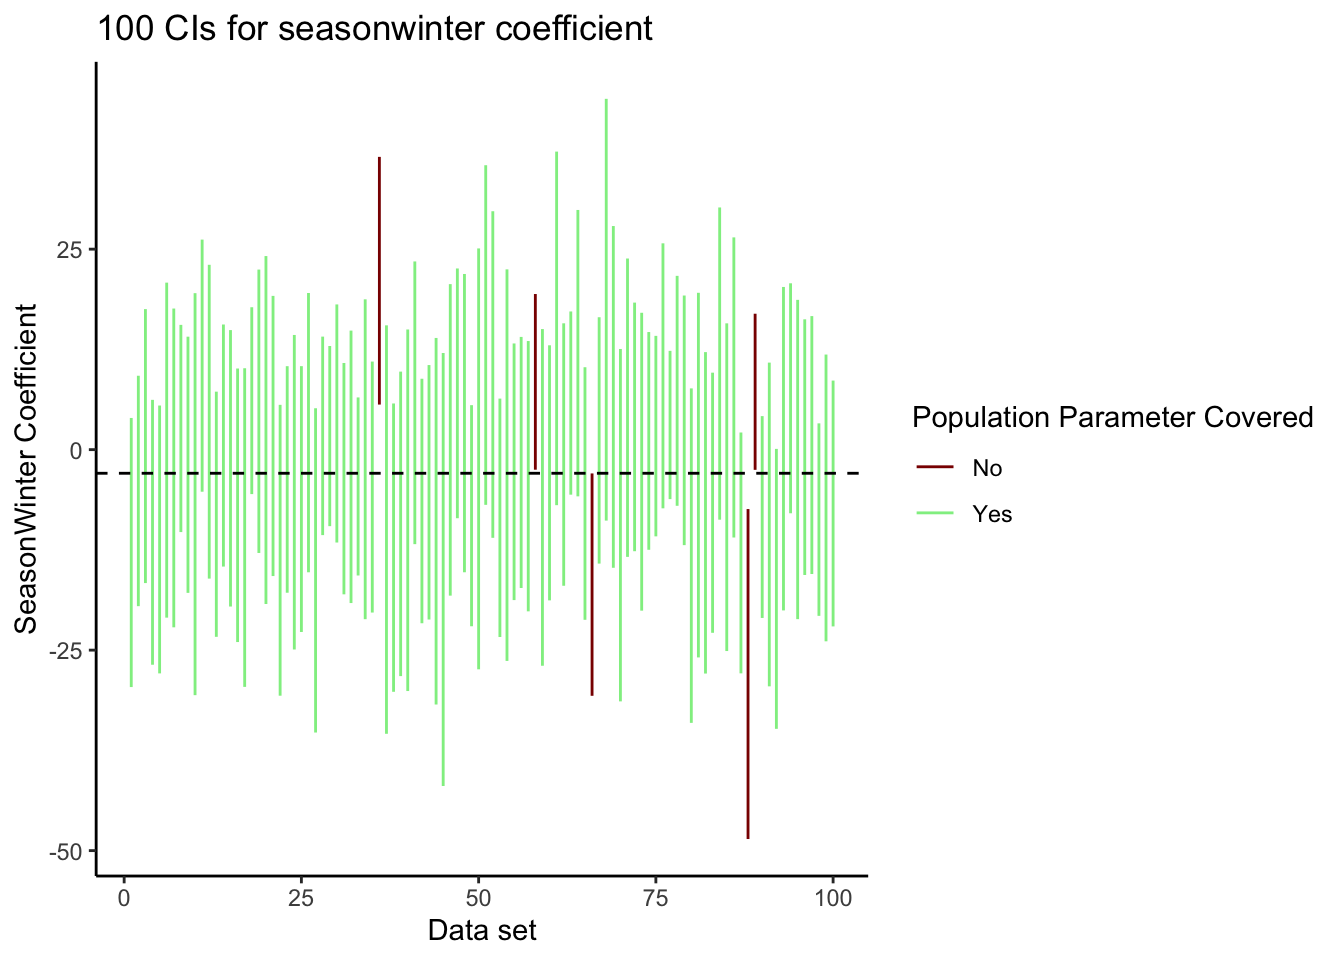
\includegraphics{02-visualization_files/figure-latex/unnamed-chunk-10-1.pdf}

\begin{reflect}
What information is highlighted when you stack the bars as compared to
having them side-by-side?
\end{reflect}

\hypertarget{stacked-bar-plot-relative-frequencies}{%
\subsection{Stacked Bar Plot (Relative Frequencies)}\label{stacked-bar-plot-relative-frequencies}}

We can adjust the stacked bar plot to make the heights the same, so that you can compare conditional distributions. For a \textbf{stacked bar plot based on proportions} (also called a \textbf{proportional bar plot}),

\begin{itemize}
\tightlist
\item
  The \textbf{relative heights} show \textbf{conditional distributions} (relative frequencies within subsets).
\item
  The \textbf{widths} of the bars have no meaning.
\end{itemize}

The code below computes the conditional distributions manually first (fractions of outcomes within the two smoking groups). Then these calculations are plotted directly.

\begin{Shaded}
\begin{Highlighting}[]
\NormalTok{Whickham }\OperatorTok
\StringTok{    }\KeywordTok{count}\NormalTok{(outcome, smoker) }\OperatorTok
\StringTok{    }\KeywordTok{group_by}\NormalTok{(smoker) }\OperatorTok
\StringTok{    }\KeywordTok{mutate}\NormalTok{(}\DataTypeTok{relfreq =}\NormalTok{ n }\OperatorTok{/}\StringTok{ }\KeywordTok{sum}\NormalTok{(n)) }\OperatorTok
\StringTok{    }\KeywordTok{ggplot}\NormalTok{(}\KeywordTok{aes}\NormalTok{(}\DataTypeTok{x =}\NormalTok{ smoker, }\DataTypeTok{y =}\NormalTok{ relfreq, }\DataTypeTok{fill =}\NormalTok{ outcome)) }\OperatorTok{+}\StringTok{ }
\StringTok{    }\KeywordTok{geom_bar}\NormalTok{(}\DataTypeTok{stat =} \StringTok{'identity'}\NormalTok{) }\OperatorTok{+}\StringTok{ }
\StringTok{    }\KeywordTok{xlab}\NormalTok{(}\StringTok{'Smoker Status'}\NormalTok{) }\OperatorTok{+}\StringTok{ }
\StringTok{    }\KeywordTok{ylab}\NormalTok{(}\StringTok{'Proportion'}\NormalTok{) }\OperatorTok{+}\StringTok{ }
\StringTok{    }\KeywordTok{scale_fill_manual}\NormalTok{(}\StringTok{'20 Year Mortality'}\NormalTok{, }\DataTypeTok{values =} \KeywordTok{c}\NormalTok{(}\StringTok{"steelblue"}\NormalTok{, }\StringTok{"lightblue"}\NormalTok{)) }\OperatorTok{+}\StringTok{ }
\StringTok{    }\KeywordTok{theme_minimal}\NormalTok{()}
\end{Highlighting}
\end{Shaded}

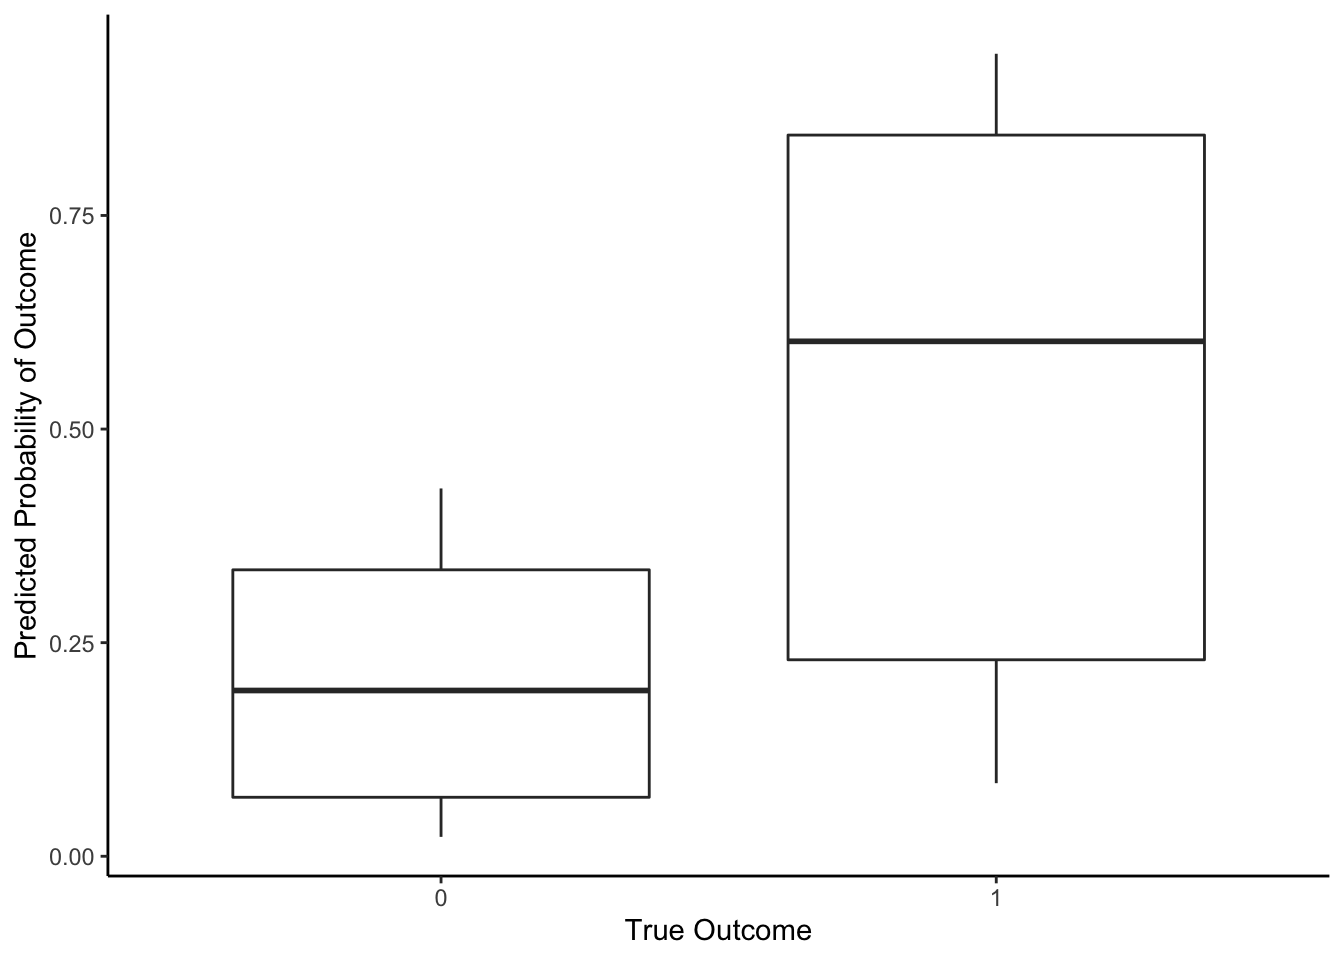
\includegraphics{02-visualization_files/figure-latex/unnamed-chunk-12-1.pdf}

Another way to make a proportional bar plot is to use the \texttt{position\ =\ "fill"}

\begin{Shaded}
\begin{Highlighting}[]
\NormalTok{Whickham }\OperatorTok
\StringTok{    }\KeywordTok{ggplot}\NormalTok{(}\KeywordTok{aes}\NormalTok{(}\DataTypeTok{x =}\NormalTok{ smoker, }\DataTypeTok{fill =}\NormalTok{ outcome)) }\OperatorTok{+}
\StringTok{    }\KeywordTok{geom_bar}\NormalTok{(}\DataTypeTok{position =} \StringTok{"fill"}\NormalTok{) }\OperatorTok{+}
\StringTok{    }\KeywordTok{xlab}\NormalTok{(}\StringTok{'Smoker Status'}\NormalTok{) }\OperatorTok{+}\StringTok{ }
\StringTok{    }\KeywordTok{ylab}\NormalTok{(}\StringTok{'Proportion'}\NormalTok{) }\OperatorTok{+}\StringTok{ }
\StringTok{    }\KeywordTok{scale_fill_manual}\NormalTok{(}\StringTok{'20 Year Mortality'}\NormalTok{, }\DataTypeTok{values =} \KeywordTok{c}\NormalTok{(}\StringTok{"steelblue"}\NormalTok{, }\StringTok{"lightblue"}\NormalTok{)) }\OperatorTok{+}\StringTok{ }
\StringTok{    }\KeywordTok{theme_minimal}\NormalTok{()}
\end{Highlighting}
\end{Shaded}

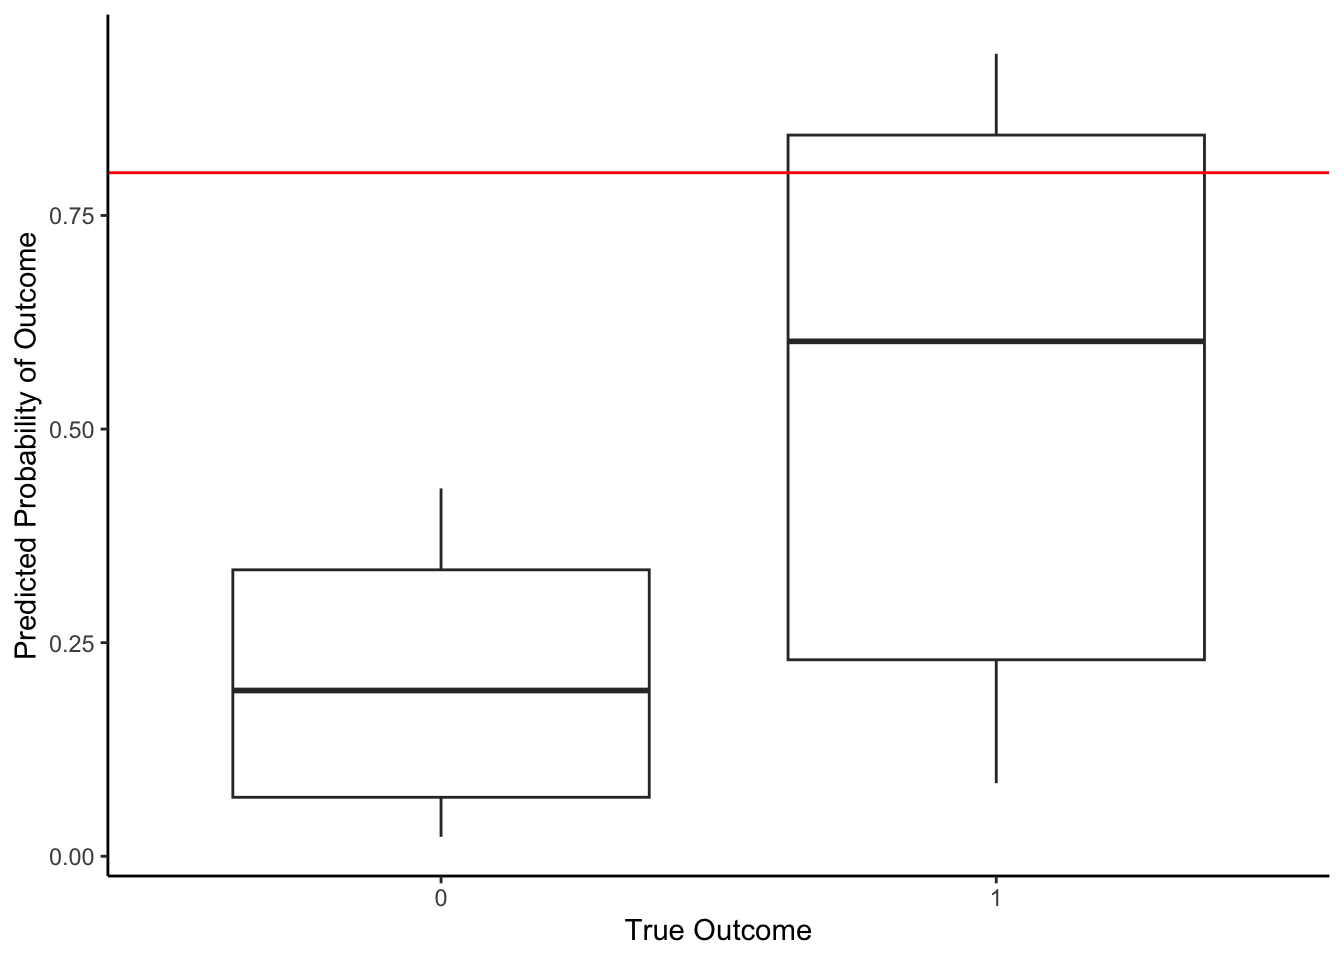
\includegraphics{02-visualization_files/figure-latex/unnamed-chunk-13-1.pdf}

\hypertarget{mosaic-plot}{%
\subsection{Mosaic Plot}\label{mosaic-plot}}

The best (Prof.~Heggeseth's opinion) graphic for two categorical variables is a variation on the stacked bar plot called a \textbf{mosaic plot}. The total heights of the bars are the same so we can compare the conditional distributions. For a \textbf{mosaic plot},

\begin{itemize}
\tightlist
\item
  The \textbf{relative height} of the bars shows the \textbf{conditional distribution} (relative frequency within subsets).
\item
  The \textbf{width} of the bars shows the \textbf{marginal distribution} (relative frequency of the X variable, ignoring the other variable).
\item
  Making mosaic plots in R requires another package: \texttt{ggmosaic}
\end{itemize}

\begin{Shaded}
\begin{Highlighting}[]
\KeywordTok{library}\NormalTok{(ggmosaic)}
\NormalTok{Whickham }\OperatorTok
\StringTok{    }\KeywordTok{ggplot}\NormalTok{() }\OperatorTok{+}
\StringTok{    }\KeywordTok{geom_mosaic}\NormalTok{(}\KeywordTok{aes}\NormalTok{(}\DataTypeTok{x =} \KeywordTok{product}\NormalTok{(outcome, smoker), }\DataTypeTok{fill =}\NormalTok{ outcome)) }\OperatorTok{+}
\StringTok{    }\KeywordTok{xlab}\NormalTok{(}\StringTok{'Smoker Status'}\NormalTok{) }\OperatorTok{+}\StringTok{ }
\StringTok{    }\KeywordTok{ylab}\NormalTok{(}\StringTok{'Counts'}\NormalTok{) }\OperatorTok{+}\StringTok{ }
\StringTok{    }\KeywordTok{scale_fill_manual}\NormalTok{(}\StringTok{'20 Year Mortality'}\NormalTok{, }\DataTypeTok{values =} \KeywordTok{c}\NormalTok{(}\StringTok{"steelblue"}\NormalTok{, }\StringTok{"lightblue"}\NormalTok{)) }\OperatorTok{+}\StringTok{ }
\StringTok{    }\KeywordTok{theme_minimal}\NormalTok{()}
\end{Highlighting}
\end{Shaded}

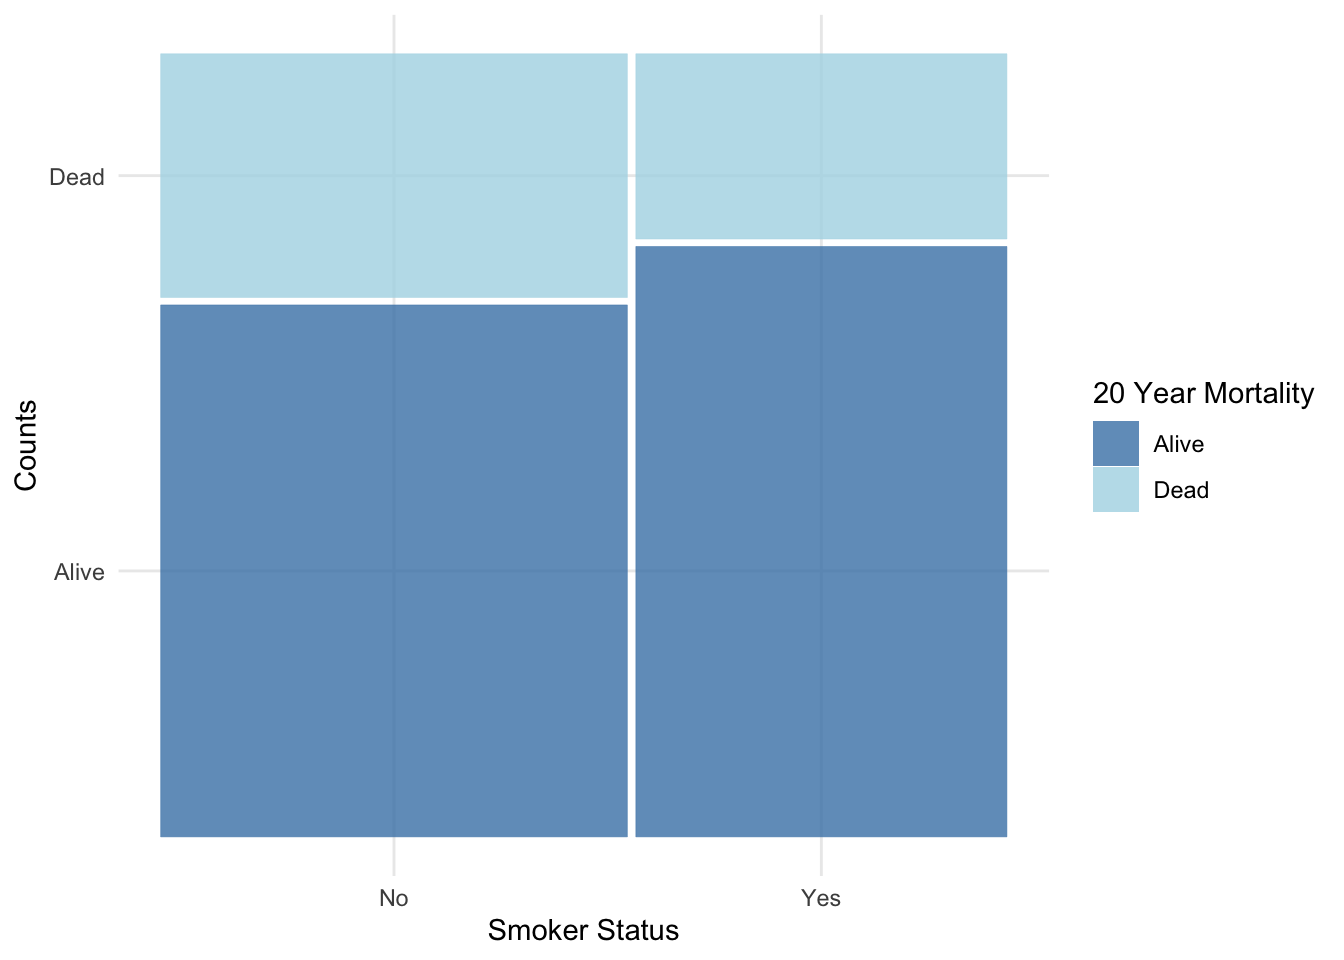
\includegraphics{02-visualization_files/figure-latex/unnamed-chunk-14-1.pdf}

\begin{reflect}
What information is highlighted when you focus on relative frequency in
the mosaic plots as compared to other bar plots?
\end{reflect}

With this type of plot, you can see that there are more non-smokers than smokers. Also, you see that there is a higher mortality rate for non-smokers.

\begin{reflect}
Does our data suggest that smoking \emph{is associated} with a lower
mortality rate? Does our data suggest that smoking \emph{reduces}
mortality? Note the difference in these two questions - the second
implies a cause and effect relationship.
\end{reflect}

Let's consider a third variable here, age distribution. We can create the same plot, separately for each age group.

\begin{Shaded}
\begin{Highlighting}[]
\NormalTok{Whickham }\OperatorTok
\StringTok{    }\KeywordTok{ggplot}\NormalTok{() }\OperatorTok{+}
\StringTok{    }\KeywordTok{geom_mosaic}\NormalTok{(}\KeywordTok{aes}\NormalTok{(}\DataTypeTok{x =} \KeywordTok{product}\NormalTok{(outcome, smoker), }\DataTypeTok{fill =}\NormalTok{ outcome)) }\OperatorTok{+}\StringTok{ }
\StringTok{    }\KeywordTok{facet_grid}\NormalTok{( . }\OperatorTok{~}\StringTok{ }\NormalTok{ageCat) }\OperatorTok{+}\StringTok{ }
\StringTok{    }\KeywordTok{xlab}\NormalTok{(}\StringTok{'Smoker Status'}\NormalTok{) }\OperatorTok{+}\StringTok{ }
\StringTok{    }\KeywordTok{ylab}\NormalTok{(}\StringTok{'Counts'}\NormalTok{) }\OperatorTok{+}\StringTok{ }
\StringTok{    }\KeywordTok{scale_fill_manual}\NormalTok{(}\StringTok{'20 Year Mortality'}\NormalTok{, }\DataTypeTok{values =} \KeywordTok{c}\NormalTok{(}\StringTok{"steelblue"}\NormalTok{, }\StringTok{"lightblue"}\NormalTok{)) }\OperatorTok{+}\StringTok{ }
\StringTok{    }\KeywordTok{theme_minimal}\NormalTok{()}
\end{Highlighting}
\end{Shaded}

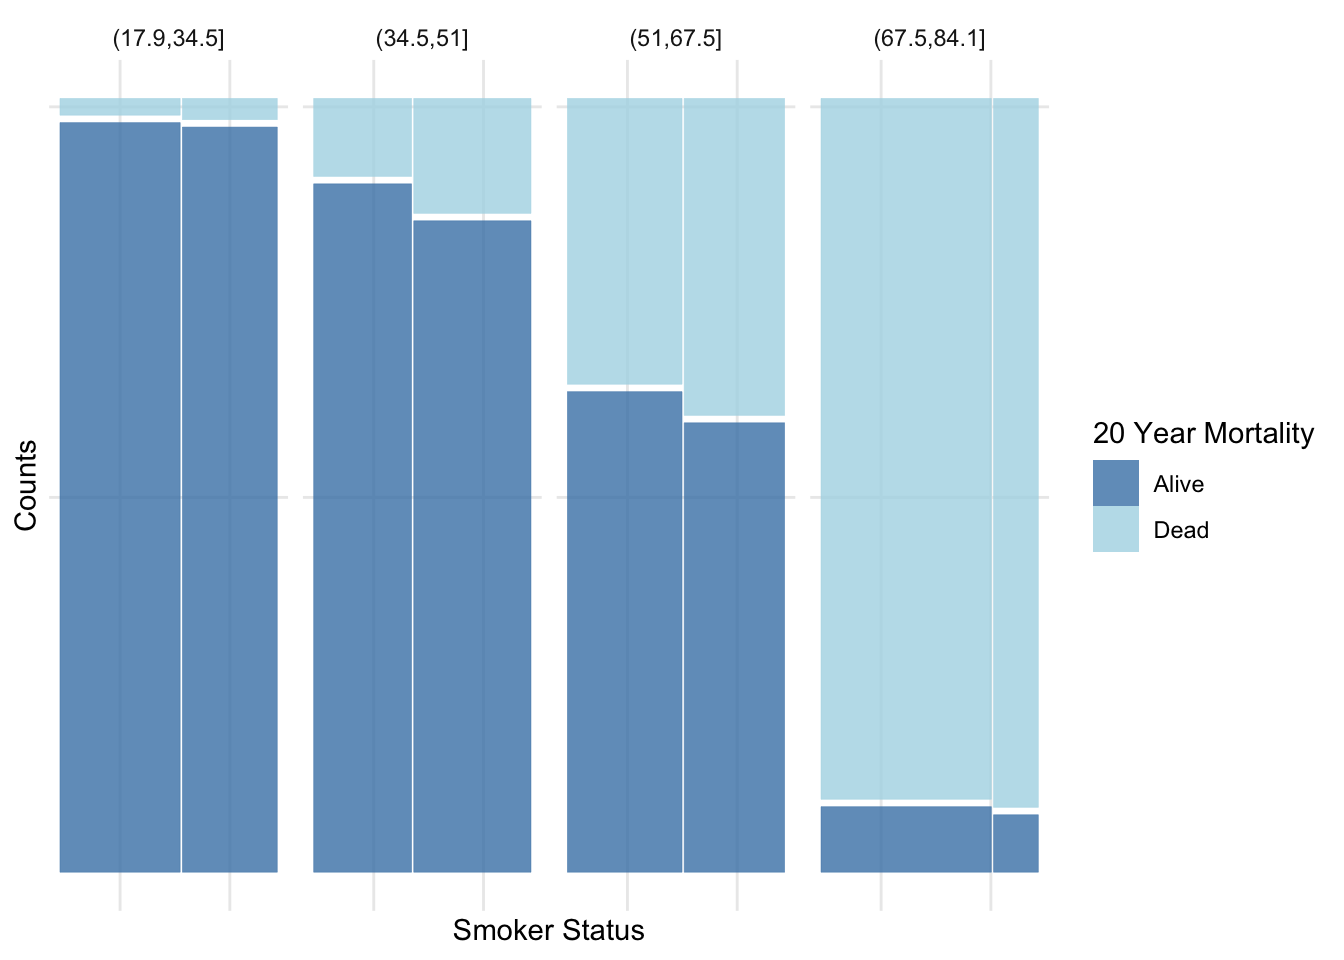
\includegraphics{02-visualization_files/figure-latex/unnamed-chunk-17-1.pdf}

\begin{reflect}
What do you gain by creating plots within subgroups?
\end{reflect}

\begin{reflect}
How is it that our conclusions are exactly the opposite if we consider
the relationship between smoking and mortality within age subsets? What
might be going on?
\end{reflect}

This is called \textbf{Simpson's Paradox,} which is a situation in which you come to two different conclusions if you look at results overall versus within subsets (e.g.~age groups).

Let's look at the marginal distribution of smoking status within each age group. For groups of people that were 68 years of age or younger, it was about 50-50 in terms of smoker vs.~non smoker. But, the oldest age group were primarily nonsmokers.

Now look at the mortality rates within each age category. The 20-year mortality rate among young people (35 or less) was very low, but mortality increases with increased age. So the oldest age group had the highest mortality rate, due primarily to their age, and also had the highest rate of non-smokers. So when we look at everyone together (not subsetting by age), it looks like smoking is associated with a lower mortality rate, when in fact age was just confounding the relationship between smoking status and mortality.

\hypertarget{one-quantitative-variable}{%
\section{One Quantitative Variable}\label{one-quantitative-variable}}

Next, we use data from one of the largest ongoing health studies in the USA, named NHANES. In particular, we will focus on data from the NHANES between 2009-2012 (Source: CDC). For more info about NHANES: \url{https://www.cdc.gov/nchs/nhanes/index.htm}.

Since sleep is vitally important to daily functioning, let's look at the number of hours of sleep respondents reported.

\hypertarget{histogram}{%
\subsection{Histogram}\label{histogram}}

One main graphical summary we use for quantitative variables is a histogram. It resembles a bar plot, but there are a few key differences:

\begin{itemize}
\tightlist
\item
  The x-axis is a number line that is divided into intervals called \textbf{bins}. Bins technically do not all have to be of equal width but almost always are. When making histograms in R, R chooses a default bin width, but you have options to change the number and/or width of the bins/intervals.
\item
  The \textbf{height} of the bars shows either the \textbf{frequency within intervals} (counts of units that fall into that bin/interval) or the \textbf{density} (fraction of units that fall into that bin/interval).
\item
  Gaps between bars are meaningful. They indicate absence of values within an interval.
\end{itemize}

\begin{Shaded}
\begin{Highlighting}[]
\KeywordTok{data}\NormalTok{(NHANES)}
\NormalTok{NHANES }\OperatorTok
\StringTok{    }\KeywordTok{ggplot}\NormalTok{(}\KeywordTok{aes}\NormalTok{(}\DataTypeTok{x =}\NormalTok{ SleepHrsNight)) }\OperatorTok{+}
\StringTok{    }\KeywordTok{geom_histogram}\NormalTok{(}\DataTypeTok{fill =} \StringTok{"steelblue"}\NormalTok{) }\OperatorTok{+}\StringTok{ }
\StringTok{    }\KeywordTok{xlab}\NormalTok{(}\StringTok{'Hours of Sleep (hours)'}\NormalTok{) }\OperatorTok{+}\StringTok{ }
\StringTok{    }\KeywordTok{ylab}\NormalTok{(}\StringTok{'Counts'}\NormalTok{) }\OperatorTok{+}\StringTok{ }
\StringTok{    }\KeywordTok{theme_minimal}\NormalTok{() }
\end{Highlighting}
\end{Shaded}

\begin{verbatim}
## `stat_bin()` using `bins = 30`. Pick better value with `binwidth`.
\end{verbatim}

\begin{verbatim}
## Warning: Removed 2245 rows containing non-finite values (stat_bin).
\end{verbatim}

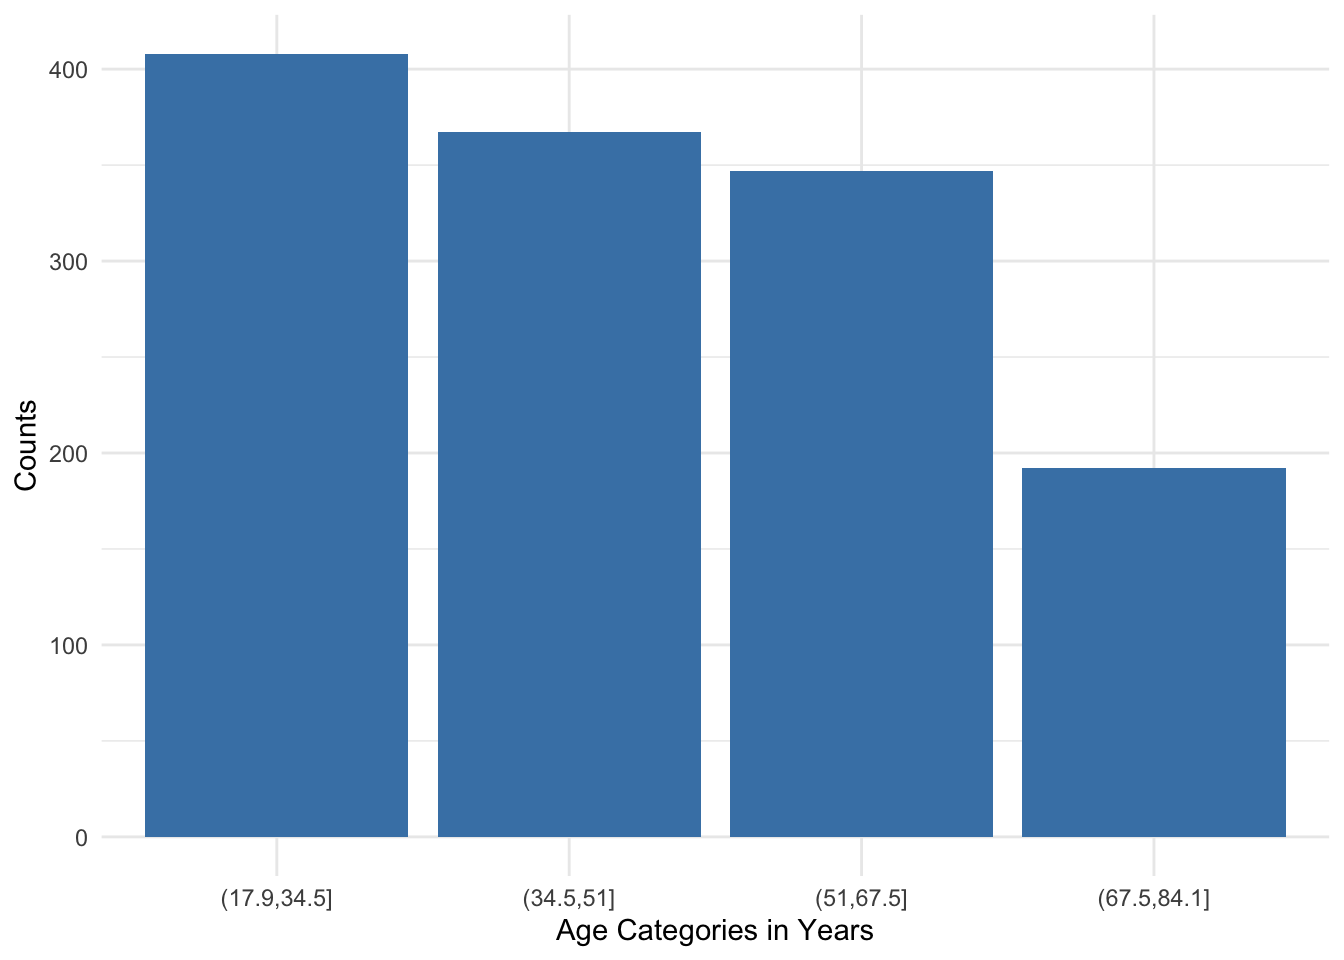
\includegraphics{02-visualization_files/figure-latex/unnamed-chunk-20-1.pdf}

Note the warning message above: ``Removed \_\_ rows containing non-finite values (stat\_bin).'' Sometimes there is missing information for a variable for some units in the dataset. We cannot plot these because we don't know their values! This warning message is just a friendly reminder from R to let you know what it is doing.

Also note the message that R gives about bin width to remind us that we can choose this if we wish. If we want to specify the width of the intervals or bins, we can specify \texttt{binwidth\ =\ DESIRED\_BIN\_WIDTH} within \texttt{geom\_histogram}.

\begin{Shaded}
\begin{Highlighting}[]
\NormalTok{NHANES }\OperatorTok
\StringTok{    }\KeywordTok{ggplot}\NormalTok{(}\KeywordTok{aes}\NormalTok{(}\DataTypeTok{x =}\NormalTok{ SleepHrsNight)) }\OperatorTok{+}
\StringTok{    }\KeywordTok{geom_histogram}\NormalTok{(}\DataTypeTok{binwidth =} \DecValTok{1}\NormalTok{, }\DataTypeTok{fill =} \StringTok{"steelblue"}\NormalTok{) }\OperatorTok{+}\StringTok{ }
\StringTok{    }\KeywordTok{xlab}\NormalTok{(}\StringTok{'Hours of Sleep (hours)'}\NormalTok{) }\OperatorTok{+}\StringTok{ }
\StringTok{    }\KeywordTok{ylab}\NormalTok{(}\StringTok{'Counts'}\NormalTok{) }\OperatorTok{+}\StringTok{ }
\StringTok{    }\KeywordTok{theme_minimal}\NormalTok{() }
\end{Highlighting}
\end{Shaded}

\begin{verbatim}
## Warning: Removed 2245 rows containing non-finite values (stat_bin).
\end{verbatim}

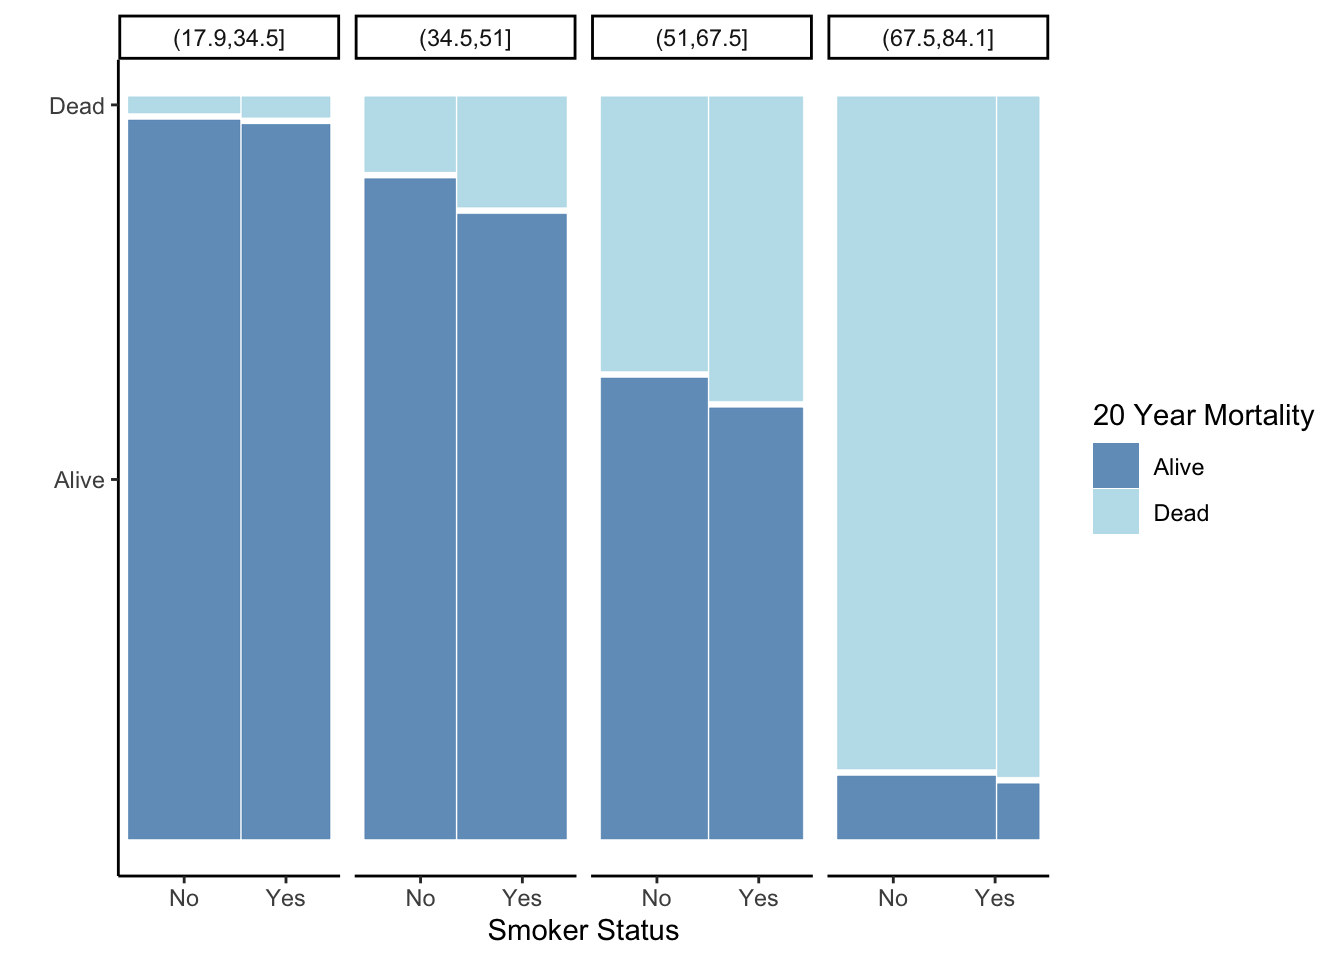
\includegraphics{02-visualization_files/figure-latex/unnamed-chunk-21-1.pdf}

Lastly, notice that the y-axis in the previous two histograms has been the counts (or frequency) within each sleep hour interval. We can adjust this to \textbf{density}, which is relative frequency adjusted for the width of interval so that the sum of the areas of the bars (height x width) equals 1.

\begin{Shaded}
\begin{Highlighting}[]
\NormalTok{NHANES }\OperatorTok
\StringTok{    }\KeywordTok{ggplot}\NormalTok{(}\KeywordTok{aes}\NormalTok{(}\DataTypeTok{x =}\NormalTok{ SleepHrsNight)) }\OperatorTok{+}
\StringTok{    }\KeywordTok{geom_histogram}\NormalTok{(}\KeywordTok{aes}\NormalTok{(}\DataTypeTok{y =}\NormalTok{ ..density..), }\DataTypeTok{binwidth =} \DecValTok{1}\NormalTok{, }\DataTypeTok{fill =} \StringTok{"steelblue"}\NormalTok{) }\OperatorTok{+}\StringTok{ }
\StringTok{    }\KeywordTok{geom_density}\NormalTok{(}\DataTypeTok{alpha =} \FloatTok{0.2}\NormalTok{, }\DataTypeTok{fill =} \StringTok{"steelblue"}\NormalTok{, }\DataTypeTok{adjust =} \DecValTok{3}\NormalTok{) }\OperatorTok{+}\StringTok{ }
\StringTok{    }\KeywordTok{xlab}\NormalTok{(}\StringTok{'Hours of Sleep (hours)'}\NormalTok{) }\OperatorTok{+}\StringTok{ }
\StringTok{    }\KeywordTok{ylab}\NormalTok{(}\StringTok{'Density'}\NormalTok{) }\OperatorTok{+}\StringTok{ }
\StringTok{    }\KeywordTok{theme_minimal}\NormalTok{() }
\end{Highlighting}
\end{Shaded}

\begin{verbatim}
## Warning: Removed 2245 rows containing non-finite values (stat_bin).
\end{verbatim}

\begin{verbatim}
## Warning: Removed 2245 rows containing non-finite values (stat_density).
\end{verbatim}

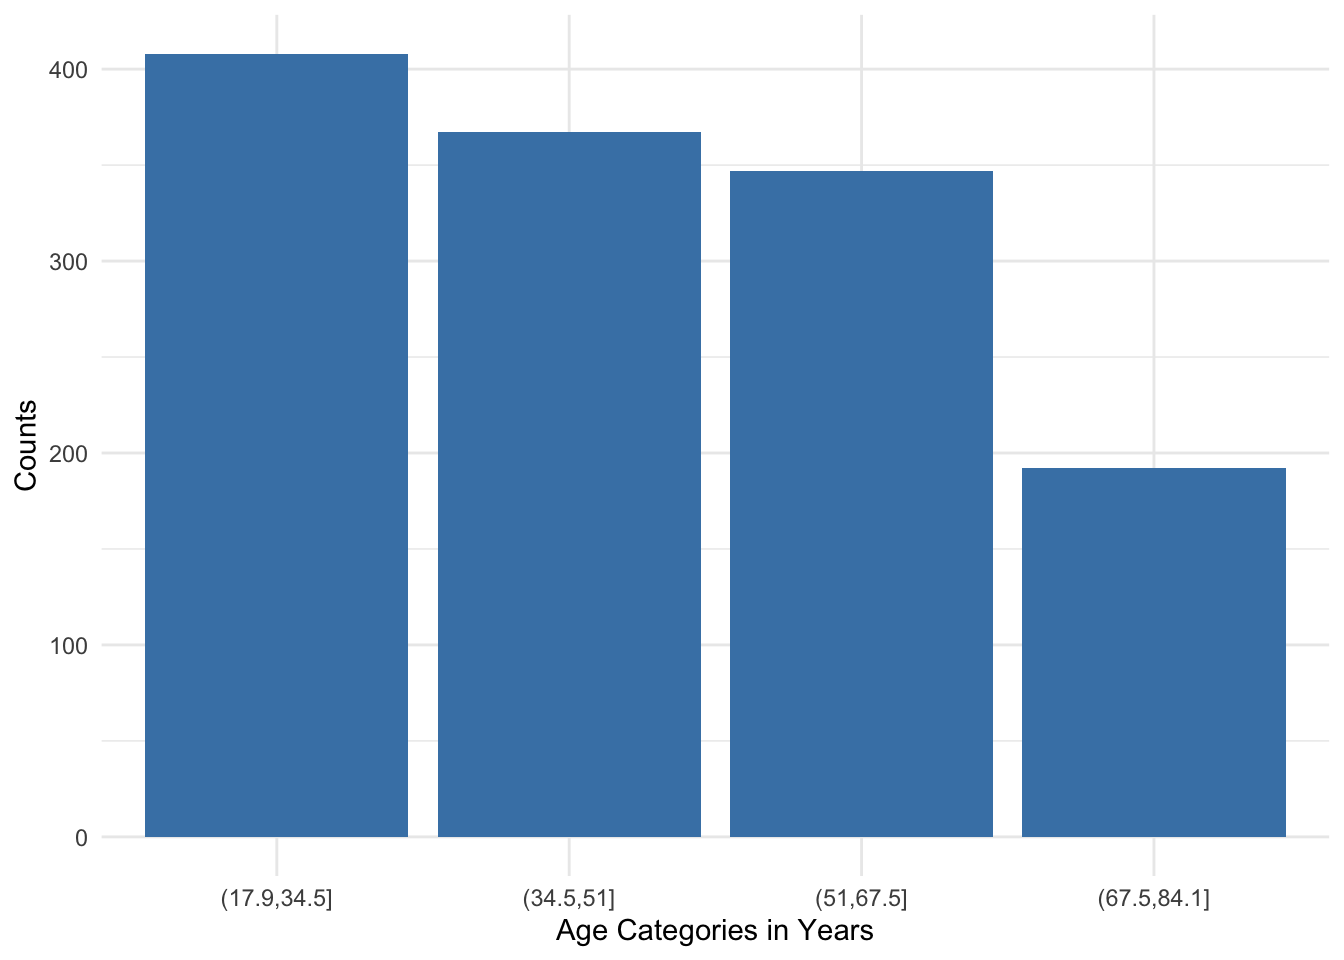
\includegraphics{02-visualization_files/figure-latex/unnamed-chunk-22-1.pdf}

The smooth curved line on this plot is called a \textbf{density plot}. It is essentially a smoother version of the histogram. Both the area under a density plot and the total area of all the rectangles in a density histogram equal 1.

When describing a distribution, we focus on three aspects of the histogram:

\begin{itemize}
\tightlist
\item
  \textbf{Shape:} Is it \textbf{symmetric} (can you fold it in half and the sides match up)? or is it \textbf{skewed to the right or left}? (A distribution is \textbf{left-skewed} if there is a long left tail and \textbf{right-skewed} if it has a long right tail.) How many \textbf{modes} (``peaks''/``bumps'' in the distribution) do you see?
\item
  \textbf{Center:} Where is a typical value located?
\item
  \textbf{Spread} (or variation): How spread out are the values? Concentrated around one or more values or spread out?
\item
  \textbf{Unusual features:} Are there \textbf{outliers} (points far from the rest)? Are there gaps? Why?
\end{itemize}

Here is another data set for comparison. Here are the annual salaries for the highest paid CEOs in 2016 (Source: NYTimes). To get the data, we are scraping the data from a NYTimes website. For fun, you can look at the code below.

\begin{Shaded}
\begin{Highlighting}[]
\NormalTok{nyturl <-}\StringTok{ 'https://www.nytimes.com/interactive/2017/05/26/business/highest-paid-ceos.html?mcubz=0'}
\NormalTok{dat <-}\StringTok{ }\KeywordTok{read_html}\NormalTok{(nyturl)}
\NormalTok{ceo <-}\StringTok{ }\NormalTok{dat }\OperatorTok\StringTok{ }
\StringTok{    }\KeywordTok{html_nodes}\NormalTok{(}\StringTok{".nytg-compensation , .nytg-year"}\NormalTok{) }\OperatorTok\StringTok{ }
\StringTok{    }\KeywordTok{html_text}\NormalTok{() }\OperatorTok\StringTok{ }
\StringTok{    }\KeywordTok{str_replace}\NormalTok{(}\StringTok{'}\CharTok{\textbackslash{}\textbackslash{}}\StringTok{$|-'}\NormalTok{,}\StringTok{''}\NormalTok{) }\CommentTok{#webscraping data }
\NormalTok{ceo <-}\StringTok{ }\KeywordTok{data.frame}\NormalTok{(}\KeywordTok{matrix}\NormalTok{(ceo,}\DataTypeTok{ncol =} \DecValTok{2}\NormalTok{,}\DataTypeTok{byrow =} \OtherTok{TRUE}\NormalTok{))}
\KeywordTok{names}\NormalTok{(ceo) <-}\StringTok{ }\KeywordTok{c}\NormalTok{(}\StringTok{'year'}\NormalTok{,}\StringTok{'salary'}\NormalTok{)}
\NormalTok{ceo}\OperatorTok{$}\NormalTok{salary <-}\StringTok{ }\KeywordTok{as.numeric}\NormalTok{(ceo}\OperatorTok{$}\NormalTok{salary) }
\NormalTok{ceo <-}\StringTok{ }\NormalTok{ceo }\OperatorTok\StringTok{ }
\StringTok{    }\KeywordTok{filter}\NormalTok{(year }\OperatorTok{==}\StringTok{ '2016'}\NormalTok{)}
\end{Highlighting}
\end{Shaded}

Let's create a density histogram of the annual salaries for the highest paid CEO's in the U.S. in 2016.

\begin{Shaded}
\begin{Highlighting}[]
\NormalTok{ceo }\OperatorTok
\StringTok{    }\KeywordTok{ggplot}\NormalTok{(}\KeywordTok{aes}\NormalTok{(}\DataTypeTok{x =}\NormalTok{ salary)) }\OperatorTok{+}
\StringTok{    }\KeywordTok{geom_histogram}\NormalTok{(}\KeywordTok{aes}\NormalTok{(}\DataTypeTok{y =}\NormalTok{ ..density..), }\DataTypeTok{binwidth =} \DecValTok{15}\NormalTok{, }\DataTypeTok{fill =} \StringTok{"steelblue"}\NormalTok{) }\OperatorTok{+}\StringTok{ }
\StringTok{    }\KeywordTok{geom_density}\NormalTok{(}\DataTypeTok{alpha =} \FloatTok{0.2}\NormalTok{, }\DataTypeTok{fill =} \StringTok{"steelblue"}\NormalTok{) }\OperatorTok{+}\StringTok{ }
\StringTok{    }\KeywordTok{xlab}\NormalTok{(}\StringTok{'Salary ($ Millions)'}\NormalTok{) }\OperatorTok{+}\StringTok{ }
\StringTok{    }\KeywordTok{ylab}\NormalTok{(}\StringTok{'Counts'}\NormalTok{) }\OperatorTok{+}\StringTok{ }
\StringTok{    }\KeywordTok{theme_minimal}\NormalTok{() }
\end{Highlighting}
\end{Shaded}

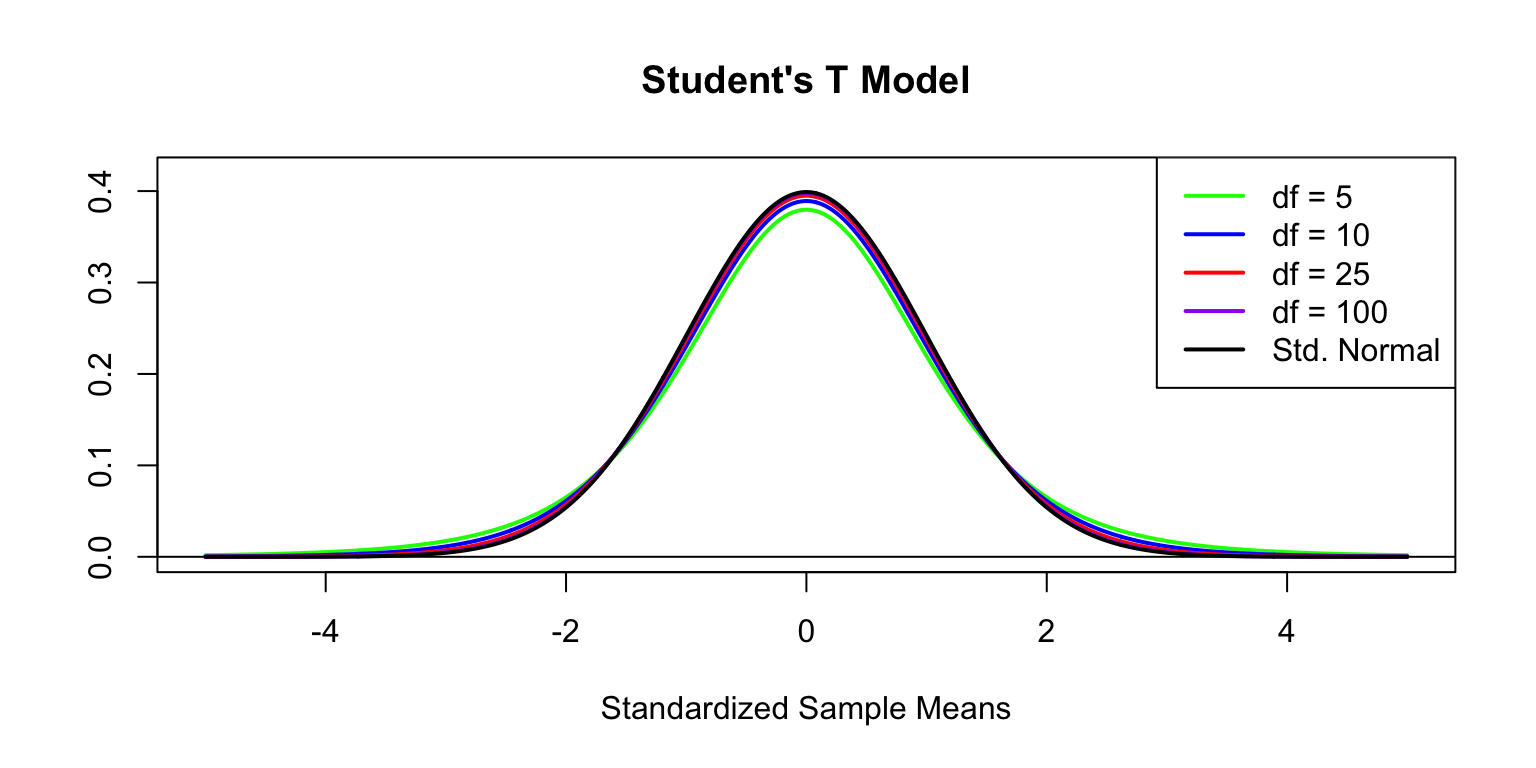
\includegraphics{02-visualization_files/figure-latex/unnamed-chunk-24-1.pdf}

We note that some of the highest salaries were close to 200 million U.S. dollars (in 2016), but the majority of the salaries in this sample are closer to 50 million U.D. dollars.

\begin{reflect}
Is this distribution of salaries left-skewed or right-skewed? In what
populations do you think salaries might be left-skewed? Right-skewed?
\end{reflect}

\hypertarget{center}{%
\subsection{Center}\label{center}}

There are some choices for numerically summarizing the center of a distribution:

\begin{itemize}
\tightlist
\item
  \textbf{Mean}: The sum of the values divided by the number of values (sample size), \(\bar{y} = \frac{\sum^n_{i=1}y_i}{n}\)

  \begin{itemize}
  \tightlist
  \item
    Sensitive to outliers, but it efficiently uses all the data
  \end{itemize}
\item
  \textbf{Median}: The ``middle'' value. The number for which half of the values are below and half are above.

  \begin{itemize}
  \tightlist
  \item
    Insensitive to outliers, but it doesn't use all the actual values
  \end{itemize}
\item
  \textbf{Trimmed means}: Drop the lowest and highest k\% and take the mean of the rest.

  \begin{itemize}
  \tightlist
  \item
    A good compromise, but not widely used.
  \end{itemize}
\end{itemize}

\begin{mathbox}
The Greek capital letter sigma, \(\sum\), is used in mathematics to
denote a sum. We let \(y_i\) represent the value of the \(i\)th person
for a variable called \(y\). So \(\sum^n_{i=1}y_i\) is the sum of all
the \(n\) values of a variable \(y\), all the way from the 1st person to
the \(n\)th person.
\end{mathbox}

We can calculate all of these in R.

\begin{itemize}
\tightlist
\item
  \textbf{Hours of sleep per night from the NHANES dataset}
\end{itemize}

\begin{Shaded}
\begin{Highlighting}[]
\NormalTok{NHANES }\OperatorTok
\StringTok{  }\KeywordTok{select}\NormalTok{(SleepHrsNight) }\OperatorTok
\StringTok{  }\KeywordTok{summary}\NormalTok{()}
\end{Highlighting}
\end{Shaded}

\begin{verbatim}
##  SleepHrsNight   
##  Min.   : 2.000  
##  1st Qu.: 6.000  
##  Median : 7.000  
##  Mean   : 6.928  
##  3rd Qu.: 8.000  
##  Max.   :12.000  
##  NA's   :2245
\end{verbatim}

\begin{Shaded}
\begin{Highlighting}[]
\NormalTok{NHANES }\OperatorTok
\StringTok{  }\KeywordTok{summarize}\NormalTok{(}\KeywordTok{mean}\NormalTok{(SleepHrsNight, }\DataTypeTok{na.rm =} \OtherTok{TRUE}\NormalTok{), }\KeywordTok{median}\NormalTok{(SleepHrsNight, }\DataTypeTok{na.rm =} \OtherTok{TRUE}\NormalTok{), }\KeywordTok{mean}\NormalTok{(SleepHrsNight, }\DataTypeTok{trim =} \FloatTok{0.05}\NormalTok{, }\DataTypeTok{na.rm =} \OtherTok{TRUE}\NormalTok{)) }\CommentTok{# na.rm = TRUE removes missing values; Trimmed mean: trim 5% from both tails before taking mean}
\end{Highlighting}
\end{Shaded}

\begin{verbatim}
## # A tibble: 1 x 3
##   `mean(SleepHrsNight, na~ `median(SleepHrsNight, ~ `mean(SleepHrsNight, trim =~
##                      <dbl>                    <int>                        <dbl>
## 1                     6.93                        7                         6.95
\end{verbatim}

\begin{itemize}
\tightlist
\item
  \textbf{CEO salary information from NYT}
\end{itemize}

\begin{Shaded}
\begin{Highlighting}[]
\NormalTok{ceo }\OperatorTok
\StringTok{  }\KeywordTok{select}\NormalTok{(salary) }\OperatorTok
\StringTok{  }\KeywordTok{summary}\NormalTok{()  }\CommentTok{# Note the differences between mean and median}
\end{Highlighting}
\end{Shaded}

\begin{verbatim}
##      salary     
##  Min.   :13.00  
##  1st Qu.:14.68  
##  Median :16.90  
##  Mean   :19.67  
##  3rd Qu.:21.20  
##  Max.   :98.00
\end{verbatim}

\begin{Shaded}
\begin{Highlighting}[]
\NormalTok{ceo }\OperatorTok
\StringTok{  }\KeywordTok{summarize}\NormalTok{(}\KeywordTok{mean}\NormalTok{(salary), }\KeywordTok{median}\NormalTok{(salary), }\KeywordTok{mean}\NormalTok{(salary, }\DataTypeTok{trim =} \FloatTok{0.05}\NormalTok{))}
\end{Highlighting}
\end{Shaded}

\begin{verbatim}
##   mean(salary) median(salary) mean(salary, trim = 0.05)
## 1      19.6715           16.9                  18.30056
\end{verbatim}

Note that the mean, median, and trimmed mean are all fairly close for the sleep hours distribution, which looks fairly symmetric.

Note also that the mean, median, and trimmed mean are somewhat different for the salary distribution, which looks right skewed. Often with right skewed distributions, the mean tends to be higher than the median because particularly large values are being summed in the calculation. The median and trimmed mean are not as sensitive to these outliers because of the sorting that is involved in their calculation.

\hypertarget{boxplot}{%
\subsection{Boxplot}\label{boxplot}}

An alternative graphical summary is a boxplot, which is a simplification of the histogram. The plot consists of

\begin{itemize}
\tightlist
\item
  A Box: the bottom of the box is at the 25th percentile (\(Q1\)) and top of the box is at the 75th percentile (\(Q3\))
\item
  Line in Box: the line in the middle of the box is at the 50th percentile, the median
\item
  Tails/Whiskers: The lines extend out from the box to most extreme observed values within \(1.5 \times (Q3-Q1)\) from \(Q1\) (bottom) or \(Q3\) (top)
\item
  Points: If any points are beyond \(1.5 \times (Q3-Q1)\) from the box edges, they are considered outliers and are plotted separately
\end{itemize}

\begin{mathbox}
A percentile is a measure indicating the value below which a given
percentage of observations in a group of observations fall. So the 25th
percentile is the value at which 25\% of the values are below. The 95th
percentile is the point at which 95\% of the observations are below.
\end{mathbox}

Here is a boxplot of the sleep amount from NHANES.

\begin{Shaded}
\begin{Highlighting}[]
\NormalTok{NHANES }\OperatorTok
\StringTok{    }\KeywordTok{ggplot}\NormalTok{(}\KeywordTok{aes}\NormalTok{(}\DataTypeTok{y =}\NormalTok{ SleepHrsNight)) }\OperatorTok{+}
\StringTok{    }\KeywordTok{geom_boxplot}\NormalTok{() }\OperatorTok{+}\StringTok{ }
\StringTok{    }\KeywordTok{ylab}\NormalTok{(}\StringTok{'Hours of Sleep (hours)'}\NormalTok{) }\OperatorTok{+}\StringTok{ }
\StringTok{    }\KeywordTok{theme_minimal}\NormalTok{() }
\end{Highlighting}
\end{Shaded}

\begin{verbatim}
## Warning: Removed 2245 rows containing non-finite values (stat_boxplot).
\end{verbatim}

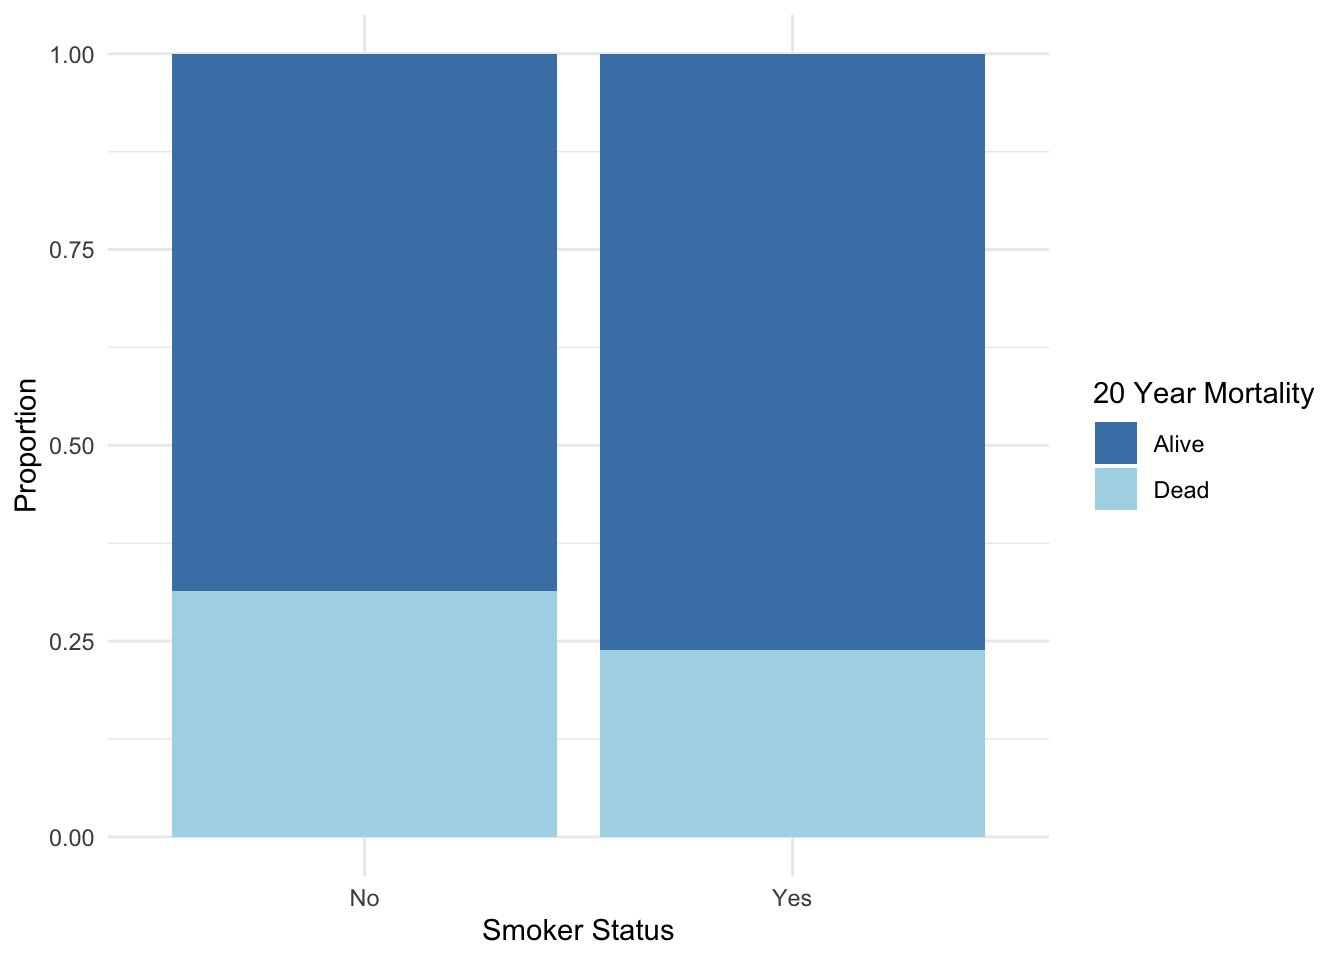
\includegraphics{02-visualization_files/figure-latex/unnamed-chunk-30-1.pdf}

Compare that to the boxplot of the CEO salaries.

\begin{Shaded}
\begin{Highlighting}[]
\NormalTok{ceo }\OperatorTok
\StringTok{    }\KeywordTok{ggplot}\NormalTok{(}\KeywordTok{aes}\NormalTok{(}\DataTypeTok{y =}\NormalTok{ salary)) }\OperatorTok{+}
\StringTok{    }\KeywordTok{geom_boxplot}\NormalTok{() }\OperatorTok{+}\StringTok{ }
\StringTok{    }\KeywordTok{ylab}\NormalTok{(}\StringTok{'Salary ($M)'}\NormalTok{) }\OperatorTok{+}\StringTok{ }
\StringTok{    }\KeywordTok{theme_minimal}\NormalTok{() }
\end{Highlighting}
\end{Shaded}

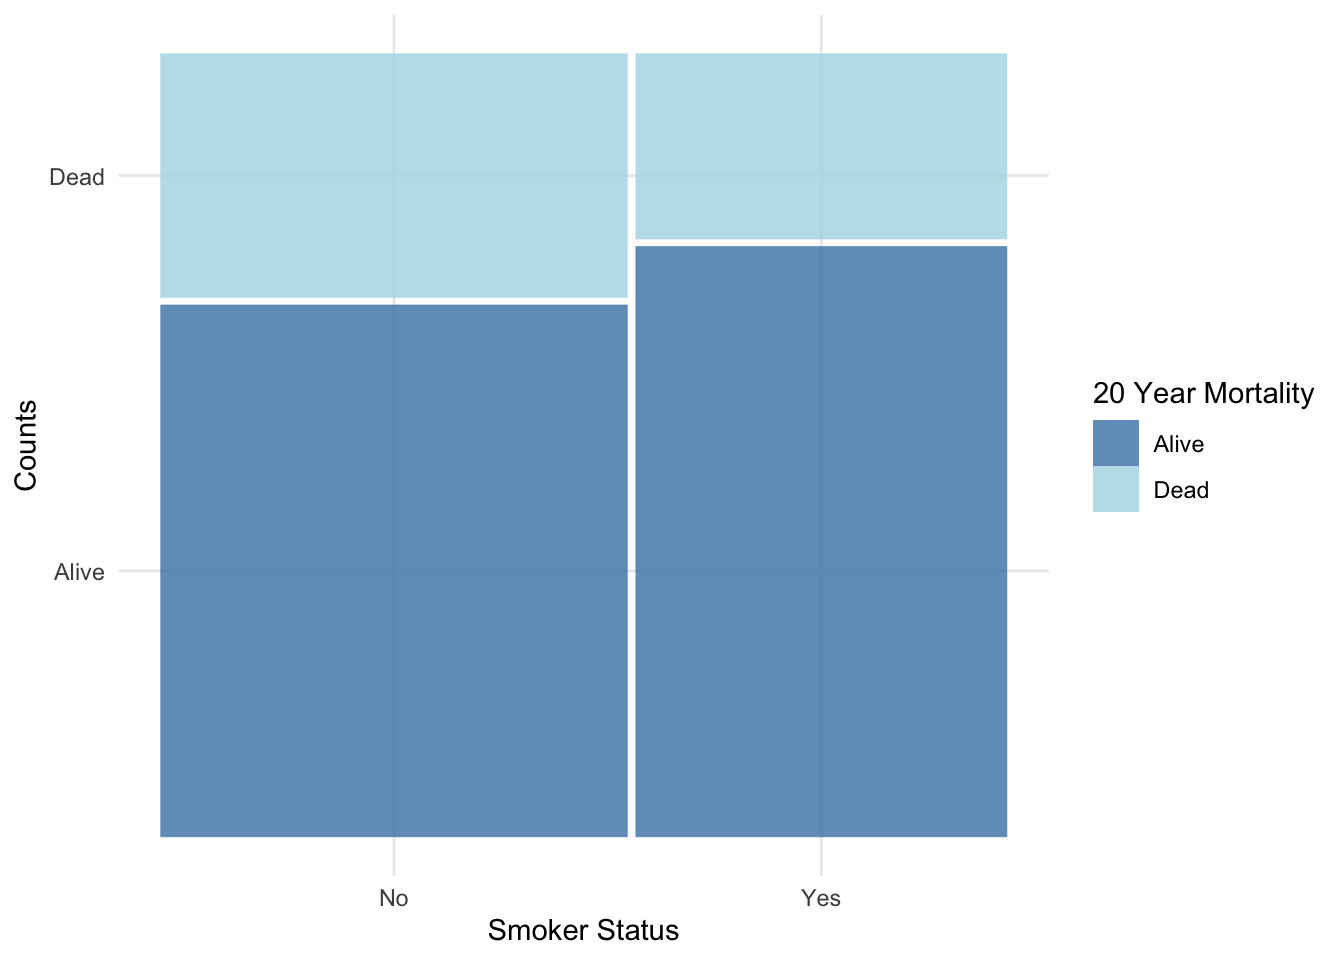
\includegraphics{02-visualization_files/figure-latex/unnamed-chunk-31-1.pdf}

Note: In these 2 plots above, the x-axis has number labels, but they don't mean anything.

Let's put the boxplots next to the histograms so we can better compare the two types of visualizations. Also, let's add the mean (red dashed), median (blue dotted), and 5\% trimmed mean (purple dash-dot) as annotations.

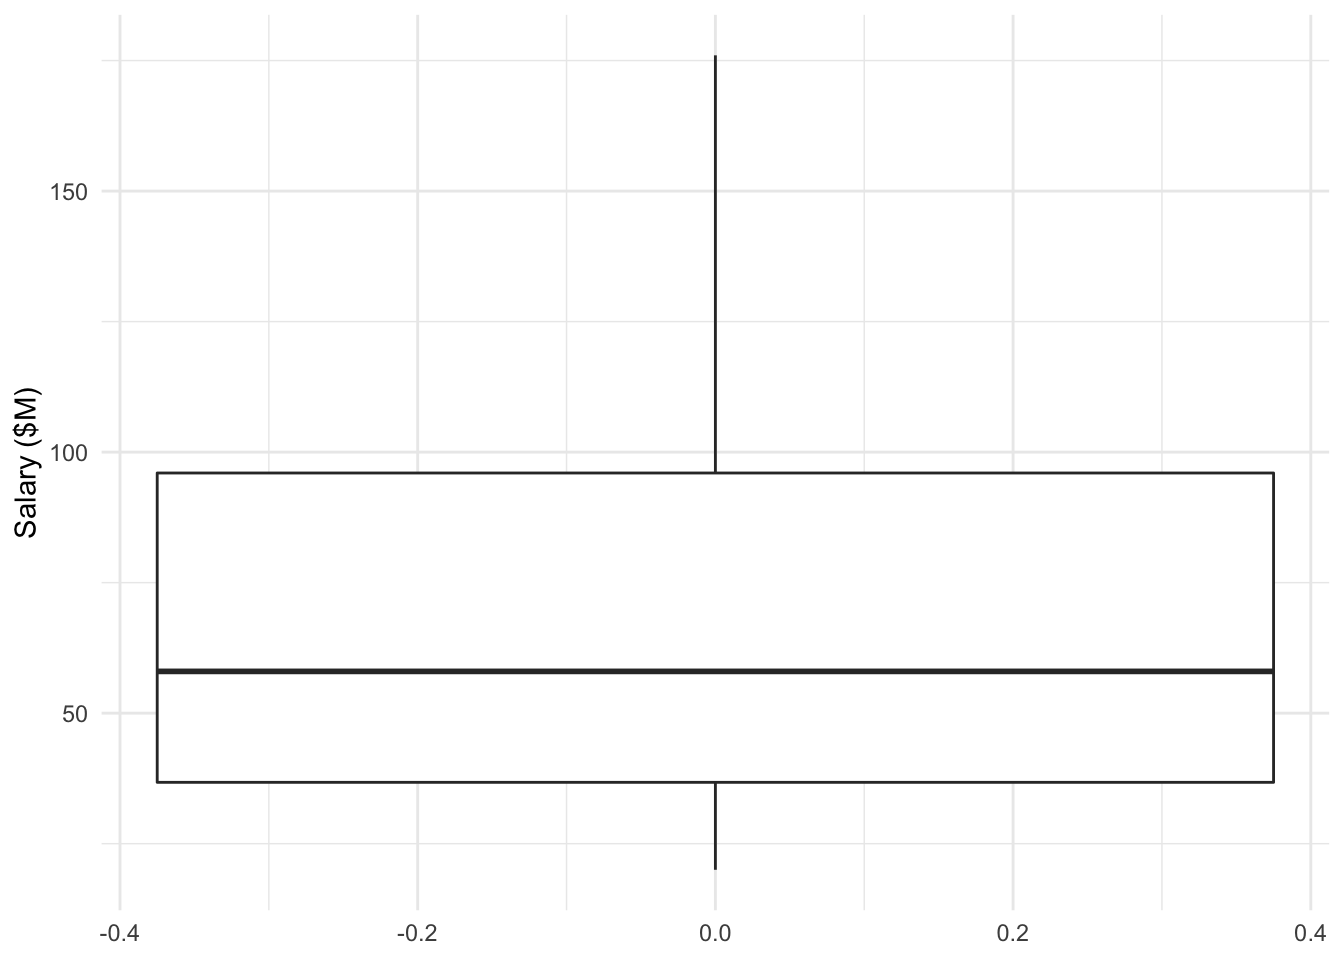
\includegraphics{02-visualization_files/figure-latex/unnamed-chunk-32-1.pdf}

For the hours of sleep, the mean, median, and 5\% trimmed mean are all pretty much the same. Note also that the distribution looks pretty symmetric based on the histogram.

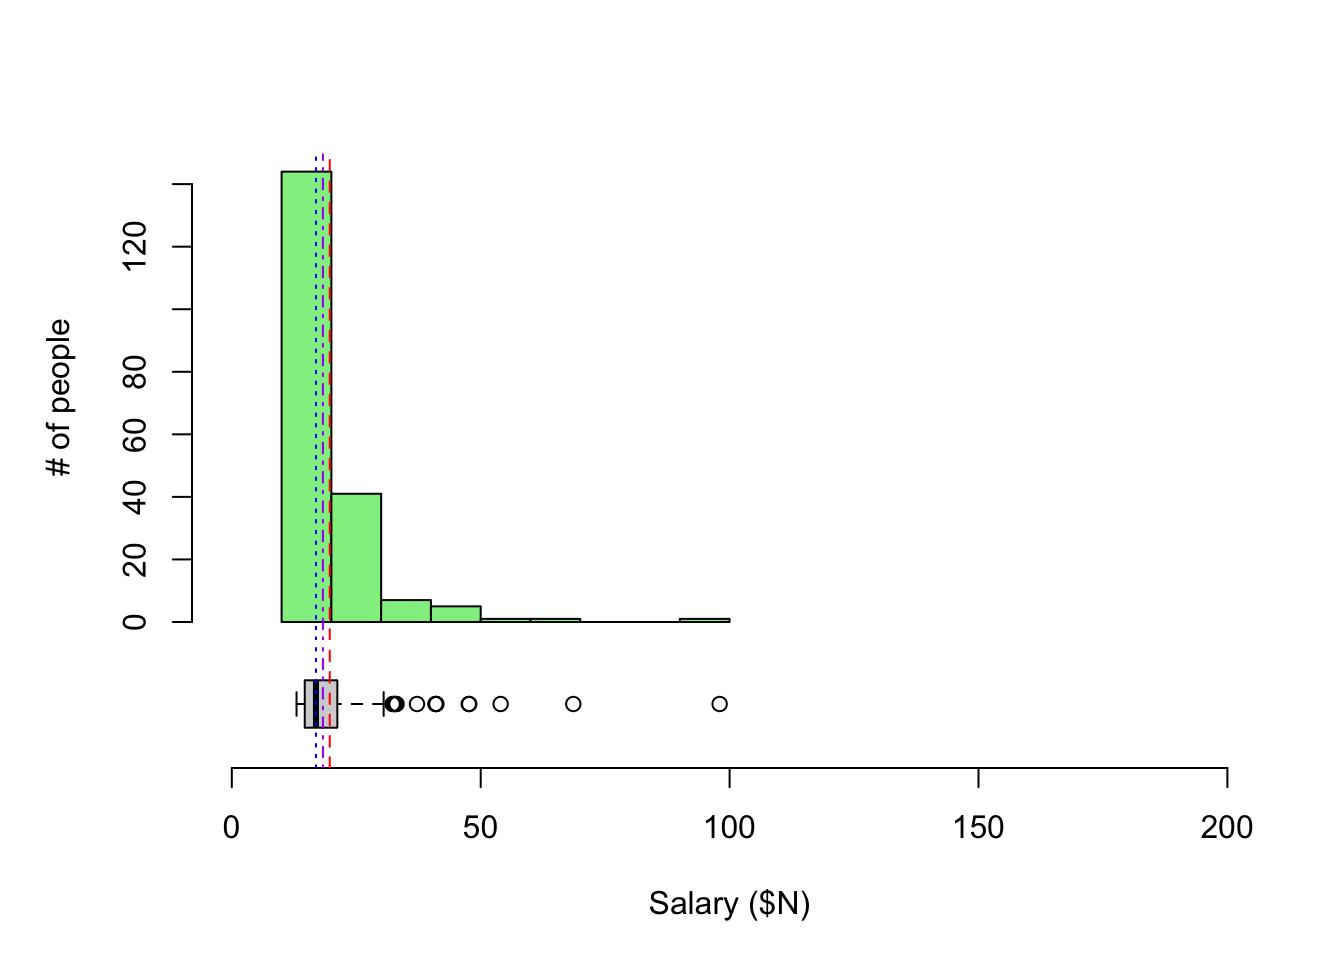
\includegraphics{02-visualization_files/figure-latex/unnamed-chunk-33-1.pdf}

For CEO salaries, the mean and 5\% trimmed mean are a bit higher than the median. \textbf{The mean is always pulled toward the long tail.}

\begin{reflect}
What would the boxplot look like if all of the values were exactly the
same? Sometimes when making multiple boxplots for each of multiple
groups, a group may only have one value or a small number of values that
all happen to be identical. What will this look like?
\end{reflect}

\hypertarget{spread}{%
\subsection{Spread}\label{spread}}

There are some choices for numerically summarizing the spread of a distribution:

\begin{itemize}
\tightlist
\item
  \textbf{Range}: the maximum value - the minimum value

  \begin{itemize}
  \tightlist
  \item
    Sensitive to the outliers since it's the difference of the extremes
  \item
    Units (e.g.~inches, pounds) are the same as the actual data
  \end{itemize}
\item
  \textbf{IQR}: the interquartile range : \(Q3 - Q1\) (75th percentile - 25th percentile).

  \begin{itemize}
  \tightlist
  \item
    Length of the box in a boxplot
  \item
    Spread of middle 50\% of data
  \item
    Like the median. Less sensitive because it doesn't use all of the data
  \item
    Units are the same as the actual data
  \end{itemize}
\item
  \textbf{Standard deviation} (SD): Root mean squared deviations from mean, \(s_y = \sqrt{\frac{\sum^n_{i=1}(y_i-\bar{y})^2}{n-1}}\)

  \begin{itemize}
  \tightlist
  \item
    Roughly the average size of deviation from the mean (\(n-1\) instead of \(n\))
  \item
    Uses all the data but very sensitive to outliers and skewed data (large values are first squared).
  \item
    Units are the same as the actual data
  \end{itemize}
\item
  \textbf{Variance}: Square of the standard deviation

  \begin{itemize}
  \tightlist
  \item
    Units are the squared version of the actual data's units (e.g.~squared inches, pounds)
  \item
    Standard deviation is preferred for interpretability of units
  \item
    Variance will come up when we discuss models in the next chapter
  \end{itemize}
\end{itemize}

We can calculate all of these in R.

\begin{itemize}
\tightlist
\item
  \textbf{Hours of sleep per night from the NHANES dataset}
\end{itemize}

\begin{Shaded}
\begin{Highlighting}[]
\NormalTok{NHANES }\OperatorTok\StringTok{ }\KeywordTok{summarize}\NormalTok{(}\KeywordTok{diff}\NormalTok{(}\KeywordTok{range}\NormalTok{(SleepHrsNight, }\DataTypeTok{na.rm =} \OtherTok{TRUE}\NormalTok{)), }\KeywordTok{IQR}\NormalTok{(SleepHrsNight, }
    \DataTypeTok{na.rm =} \OtherTok{TRUE}\NormalTok{), }\KeywordTok{sd}\NormalTok{(SleepHrsNight, }\DataTypeTok{na.rm =} \OtherTok{TRUE}\NormalTok{), }\KeywordTok{var}\NormalTok{(SleepHrsNight, }\DataTypeTok{na.rm =} \OtherTok{TRUE}\NormalTok{))}
\end{Highlighting}
\end{Shaded}

\begin{verbatim}
## # A tibble: 1 x 4
##   `diff(range(SleepHr~ `IQR(SleepHrsNight~ `sd(SleepHrsNight~ `var(SleepHrsNigh~
##                  <int>               <dbl>              <dbl>              <dbl>
## 1                   10                   2               1.35               1.81
\end{verbatim}

\begin{Shaded}
\begin{Highlighting}[]
\CommentTok{# range gives max and min; take difference betwee max and min IQR = Q3-Q1 sd =}
\CommentTok{# standard deviation var = variance}
\end{Highlighting}
\end{Shaded}

\begin{itemize}
\tightlist
\item
  \textbf{CEO salary information from NYT}
\end{itemize}

\begin{Shaded}
\begin{Highlighting}[]
\NormalTok{ceo }\OperatorTok\StringTok{ }\KeywordTok{summarize}\NormalTok{(}\KeywordTok{diff}\NormalTok{(}\KeywordTok{range}\NormalTok{(salary)), }\KeywordTok{IQR}\NormalTok{(salary), }\KeywordTok{sd}\NormalTok{(salary), }\KeywordTok{var}\NormalTok{(salary))}
\end{Highlighting}
\end{Shaded}

\begin{verbatim}
##   diff(range(salary)) IQR(salary) sd(salary) var(salary)
## 1                  85       6.525   9.452969    89.35863
\end{verbatim}

\hypertarget{intro-zscore}{%
\subsection{Some data accounting}\label{intro-zscore}}

We've looked at different measures of the spread of a distribution. Do some measures of spread encompass a lot of the data? Just a little? Can we be more precise about how much of the data is encompassed by intervals created from different spread measures?

\begin{Shaded}
\begin{Highlighting}[]
\NormalTok{x <-}\StringTok{ }\KeywordTok{rnorm}\NormalTok{(}\DecValTok{1500}\NormalTok{)}
\KeywordTok{boxplot}\NormalTok{(x, }\DataTypeTok{horizontal =} \OtherTok{TRUE}\NormalTok{, }\DataTypeTok{xlab =} \StringTok{"Generated Data"}\NormalTok{)}
\KeywordTok{abline}\NormalTok{(}\DataTypeTok{v =} \KeywordTok{range}\NormalTok{(x), }\DataTypeTok{col =} \StringTok{"blue"}\NormalTok{, }\DataTypeTok{lty =} \DecValTok{3}\NormalTok{)}
\KeywordTok{abline}\NormalTok{(}\DataTypeTok{v =} \KeywordTok{quantile}\NormalTok{(x, }\KeywordTok{c}\NormalTok{(}\FloatTok{0.25}\NormalTok{, }\FloatTok{0.75}\NormalTok{)), }\DataTypeTok{col =} \StringTok{"purple"}\NormalTok{, }\DataTypeTok{lty =} \DecValTok{1}\NormalTok{)}
\KeywordTok{abline}\NormalTok{(}\DataTypeTok{v =} \KeywordTok{c}\NormalTok{(}\KeywordTok{mean}\NormalTok{(x) }\OperatorTok{-}\StringTok{ }\KeywordTok{sd}\NormalTok{(x), }\KeywordTok{mean}\NormalTok{(x) }\OperatorTok{+}\StringTok{ }\KeywordTok{sd}\NormalTok{(x)), }\DataTypeTok{col =} \StringTok{"green"}\NormalTok{, }\DataTypeTok{lty =} \DecValTok{2}\NormalTok{)}
\end{Highlighting}
\end{Shaded}

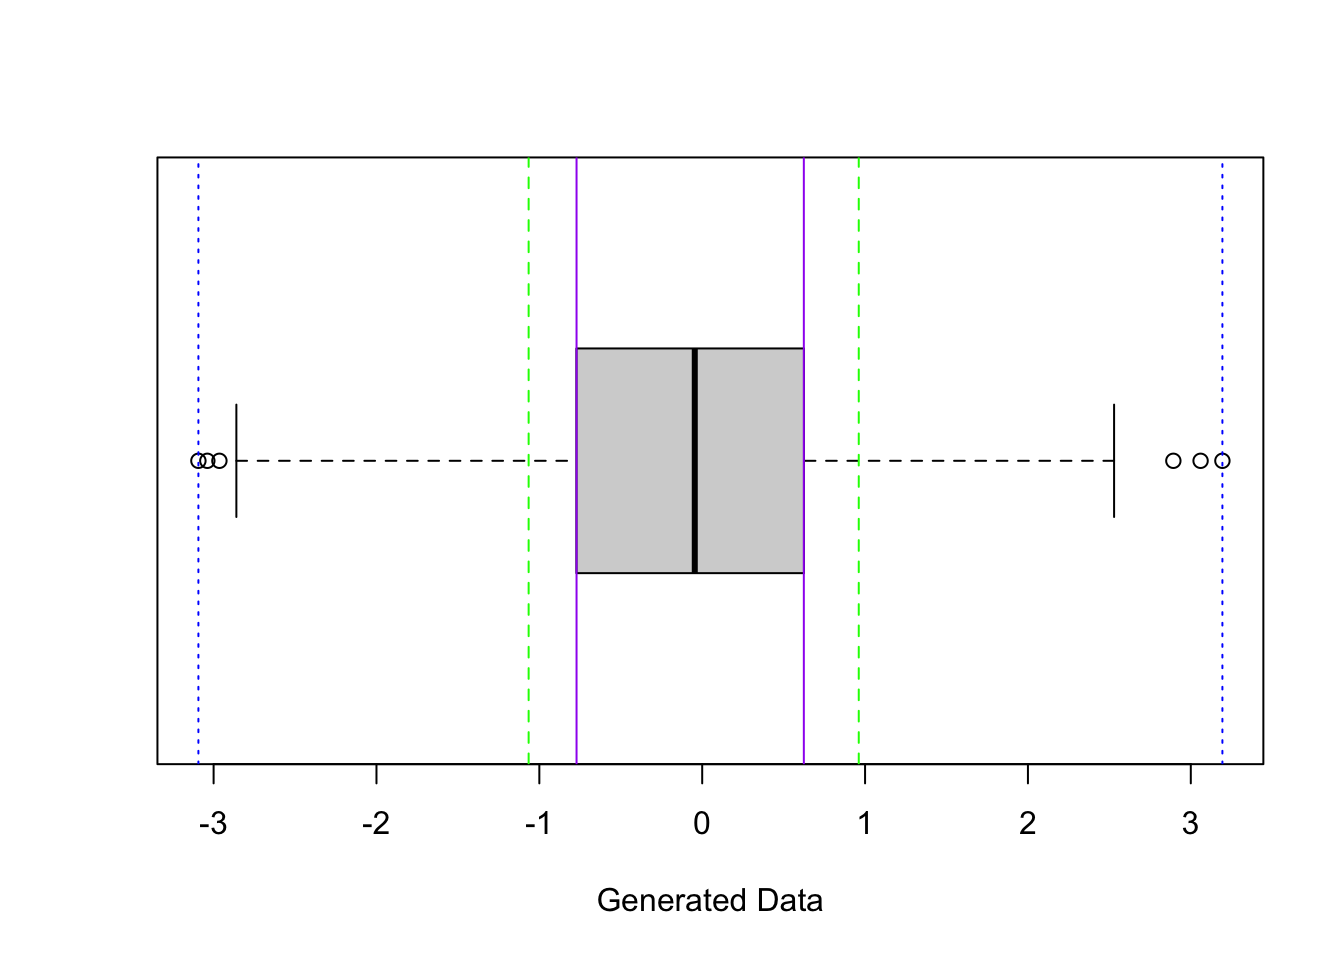
\includegraphics{02-visualization_files/figure-latex/unnamed-chunk-37-1.pdf}

\begin{reflect}
What percentage of the data is between the blue dotted lines (length of
interval is range)?

What percentage of the data is between the purple solid lines (length of
interval is IQR)?

What percentage of the data is between the green dashed lines (length of
interval is 2*SD)?
\end{reflect}

The code below computes the fraction of data points, \texttt{x}, that fall between the lower bound of 1 SD below the mean and the upper bound of 1 SD above the mean.

\begin{Shaded}
\begin{Highlighting}[]
\KeywordTok{sum}\NormalTok{(x }\OperatorTok{>}\StringTok{ }\KeywordTok{mean}\NormalTok{(x) }\OperatorTok{-}\StringTok{ }\KeywordTok{sd}\NormalTok{(x) }\OperatorTok{&}\StringTok{ }\NormalTok{x }\OperatorTok{<}\StringTok{ }\KeywordTok{mean}\NormalTok{(x) }\OperatorTok{+}\StringTok{ }\KeywordTok{sd}\NormalTok{(x))}\OperatorTok{/}\KeywordTok{length}\NormalTok{(x)}
\end{Highlighting}
\end{Shaded}

\begin{verbatim}
## [1] 0.6833333
\end{verbatim}

So with this data set, about 68\% of the data values fall within 1 SD of the mean.

\begin{reflect}
If we had a different data set, do you know that answer to the following
questions? \emph{You should know the answer to 2 of them at this
point\ldots{}}

\begin{itemize}
\item
  What percentage of the data would be between the minimum and maximum
  (blue dotted lines above)?
\item
  What percentage of the data would be between bottom and top of the box
  (purple solid lines above)?
\item
  What percentage of the data would be between 1 SD below the mean and 1
  SD above the mean (green dashed lines)?
\end{itemize}
\end{reflect}

\hypertarget{z-scores}{%
\subsection{Z-scores}\label{z-scores}}

How do you decide when an outlier is really unusual (think: athletic victory being very impressive or a data point that may be a typing error such as a human weight of 3000 lbs)?

If the observation is far from the rest of the measurements in the data, we tend to say that the value is unusual. We want to quantify this idea of ``unusual''.

To do this, we often calculate a \textbf{z-score}, a standardized data value which we denote with the letter, \(z\). To calculate a z-score,

\begin{itemize}
\tightlist
\item
  Calculate how far an observation, \(y\), is below (or above) the mean of the sample, denoted as \(\bar{y}\).
\item
  Then divide the difference by the standard deviation (measure of spread), denoted as \(s_y\).
\end{itemize}

\[ z = \frac{y - \bar{y}}{s_y} \]

The z-score tells you how many standard deviations the observation is above or below the mean.

\begin{reflect}
Say that you got a z-score of 1 on an exam with mean = 80 and SD = 5.
That means that you got an 85 on the exam because your exam is one SD
above the mean (\(mean + z \times SD = 80 + 1 \times 5\)).

If you got a z = -2 on an exam with mean = 80 and SD = 5, that means you
got a 70 on the exam because your exam is two SD below the mean
(\(mean + z \times SD = 80 + -2 \times 5\)).
\end{reflect}

In general, it is quite common to have z-scores between -3 and 3, but fairly unusual to have them greater than 3 or less than -3.

Often, if you have data with a \textbf{unimodal, symmetric distribution},

\begin{itemize}
\tightlist
\item
  about 68\% of the z-scores are between -1 and 1,
\item
  about 95\% of the z-scores are between -2 and 2,
\item
  about 99.7\% of the z-scores are between -3 and 3.
\end{itemize}

This is not true for every histogram, but it will be true for a particularly special distribution that we will see later when we cover models. (This distribution is called the \textbf{normal distribution} or \textbf{Gaussian distribution}.)

However, we do know that z-scores of 5 or larger in magnitude (ignoring negative sign) are very unusual, no matter the shape of the histogram/distribution. For those inclined, see the mathematical theorem below that tells us this.

\begin{mathbox}
(Optional) Chebyshev's inequality gives bounds for the percentages no
matter the shape of the distribution. It states that for any real number
\(k\) \textgreater{} 0, the chance of getting a z-score greater in
magnitude (ignoring the negative sign) than \(k\) is less than or equal
to \(1/k^2\),

\[P\left(|Z| \geq k\right) \leq \frac{1}{k^2}\] where
\(Z = \frac{|X - \mu|}{\sigma}\) is a z-score, \(\mu\) is the mean, and
\(\sigma\) is the standard deviation.

If we plug in values for \(k\), we see that the chance of getting a
z-score

\begin{itemize}
\tightlist
\item
  at least 3 in magnitude (\textgreater{} 3 or \textless{} -3) is less
  than \((1/3^2) = 0.11 = 11\%\).
\item
  at least 4 in magnitude (\textgreater{} 4 or \textless{} -4) is less
  than \((1/4^2) = 0.06 = 6\%\).
\item
  at least 5 in magnitude (\textgreater{} 5 or \textless{} -5) is less
  than \((1/5^2) = 0.04 = 4\%\).
\end{itemize}

This is true for any shaped distribution (skewed, bimodal, etc.). See
\href{https://en.wikipedia.org/wiki/Markov\%27s_inequality}{proof here}
based on probability theory.
\end{mathbox}

In summary, for a quantitative variable,

\begin{itemize}
\tightlist
\item
  Use a histogram to display the distribution of one variable and describe the shape and any unusual features.
\item
  For ``well-behaved'' distributions (symmetric, unimodal, no outliers), use the mean and standard deviation to describe the center and spread. Then z-scores will roughly follow the 68-95-99.7 rule stated above.
\item
  For other distributions (skewed or bimodal), use the IQR and median. You can report both mean and median, but it's usually a good idea to state why.
\end{itemize}

\hypertarget{one-quant.-and-one-cat.-variable}{%
\section{One Quant. and One Cat. Variable}\label{one-quant.-and-one-cat.-variable}}

Let's return to the NHANES data. We noticed variation in the amount people sleep. Why do some people sleep more than others? Are there any other characteristics that may be able to \emph{explain that variation}?

Let's look at the distribution of hours of sleep at night within subsets or groups of the NHANES data.

\hypertarget{multiple-histograms}{%
\subsection{Multiple Histograms}\label{multiple-histograms}}

\textbf{Does the recorded binary gender explain the variability in the hours of sleep?}

\begin{reflect}
What are the \emph{ethical implications} of collecting gender identity
as a binary variable (male/female) if some individuals do not identify
with these categories?

What might be the \emph{causal mechanism} between gender identity and
sleep? Might you be more interested in hormone levels, which might not
necessarily correspond to gender identity? How might you change the data
collection procedure so that the data can address the underlying
research question?
\end{reflect}

Let's make a histogram for each gender category by adding \texttt{facet\_grid(.\ \textasciitilde{}\ Gender)} which separates the data into groups defined by the variable, \texttt{Gender}, and creates two plots along the x-axis.

\begin{Shaded}
\begin{Highlighting}[]
\NormalTok{NHANES }\OperatorTok
\StringTok{    }\KeywordTok{ggplot}\NormalTok{(}\KeywordTok{aes}\NormalTok{(}\DataTypeTok{x =}\NormalTok{ SleepHrsNight)) }\OperatorTok{+}
\StringTok{    }\KeywordTok{geom_histogram}\NormalTok{(}\DataTypeTok{binwidth =} \DecValTok{1}\NormalTok{, }\DataTypeTok{fill =} \StringTok{"steelblue"}\NormalTok{) }\OperatorTok{+}\StringTok{ }
\StringTok{    }\KeywordTok{xlab}\NormalTok{(}\StringTok{'Hours of Sleep (hours)'}\NormalTok{) }\OperatorTok{+}\StringTok{ }
\StringTok{    }\KeywordTok{facet_grid}\NormalTok{(. }\OperatorTok{~}\StringTok{ }\NormalTok{Gender) }\OperatorTok{+}\StringTok{ }
\StringTok{    }\KeywordTok{theme_minimal}\NormalTok{()}
\end{Highlighting}
\end{Shaded}

\begin{verbatim}
## Warning: Removed 2245 rows containing non-finite values (stat_bin).
\end{verbatim}

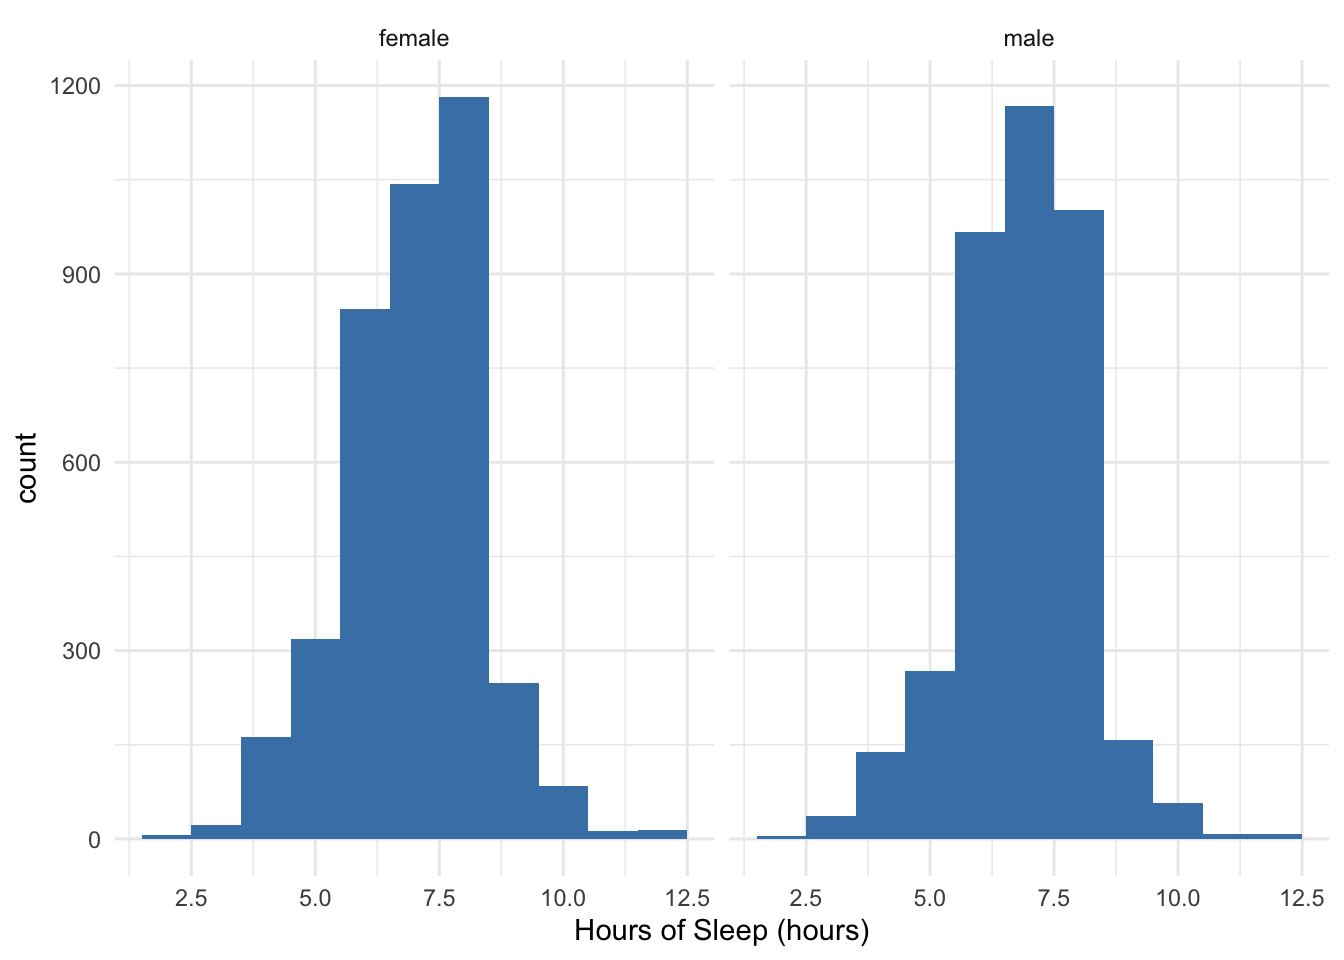
\includegraphics{02-visualization_files/figure-latex/unnamed-chunk-44-1.pdf}

\begin{reflect}
Do you notice any differences in sleep hour distributions between males
and females?

What is easy to compare and what is hard to compare between the two
histograms?
\end{reflect}

\textbf{Does the number of children a woman has explain the variability in the hours of sleep?}

\begin{reflect}
Who have we excluded from our analysis by asking this question?
\end{reflect}

\begin{Shaded}
\begin{Highlighting}[]
\NormalTok{NHANES }\OperatorTok
\StringTok{    }\KeywordTok{filter}\NormalTok{(}\OperatorTok{!}\KeywordTok{is.na}\NormalTok{(nBabies)) }\OperatorTok\StringTok{ }
\StringTok{    }\KeywordTok{ggplot}\NormalTok{(}\KeywordTok{aes}\NormalTok{(}\DataTypeTok{x =}\NormalTok{ SleepHrsNight)) }\OperatorTok{+}
\StringTok{    }\KeywordTok{geom_histogram}\NormalTok{(}\DataTypeTok{binwidth =} \DecValTok{1}\NormalTok{, }\DataTypeTok{fill =} \StringTok{"steelblue"}\NormalTok{) }\OperatorTok{+}\StringTok{ }
\StringTok{    }\KeywordTok{xlab}\NormalTok{(}\StringTok{'Hours of Sleep (hours)'}\NormalTok{) }\OperatorTok{+}\StringTok{ }
\StringTok{    }\KeywordTok{facet_wrap}\NormalTok{(. }\OperatorTok{~}\StringTok{ }\KeywordTok{factor}\NormalTok{(nBabies), }\DataTypeTok{ncol =} \DecValTok{4}\NormalTok{) }\OperatorTok{+}\StringTok{ }
\StringTok{    }\KeywordTok{theme}\NormalTok{(}\DataTypeTok{axis.text.x =} \KeywordTok{element_text}\NormalTok{(}\DataTypeTok{angle =} \DecValTok{90}\NormalTok{, }\DataTypeTok{hjust =} \DecValTok{1}\NormalTok{)) }\OperatorTok{+}
\StringTok{    }\KeywordTok{theme_minimal}\NormalTok{()}
\end{Highlighting}
\end{Shaded}

\begin{verbatim}
## Warning: Removed 8 rows containing non-finite values (stat_bin).
\end{verbatim}

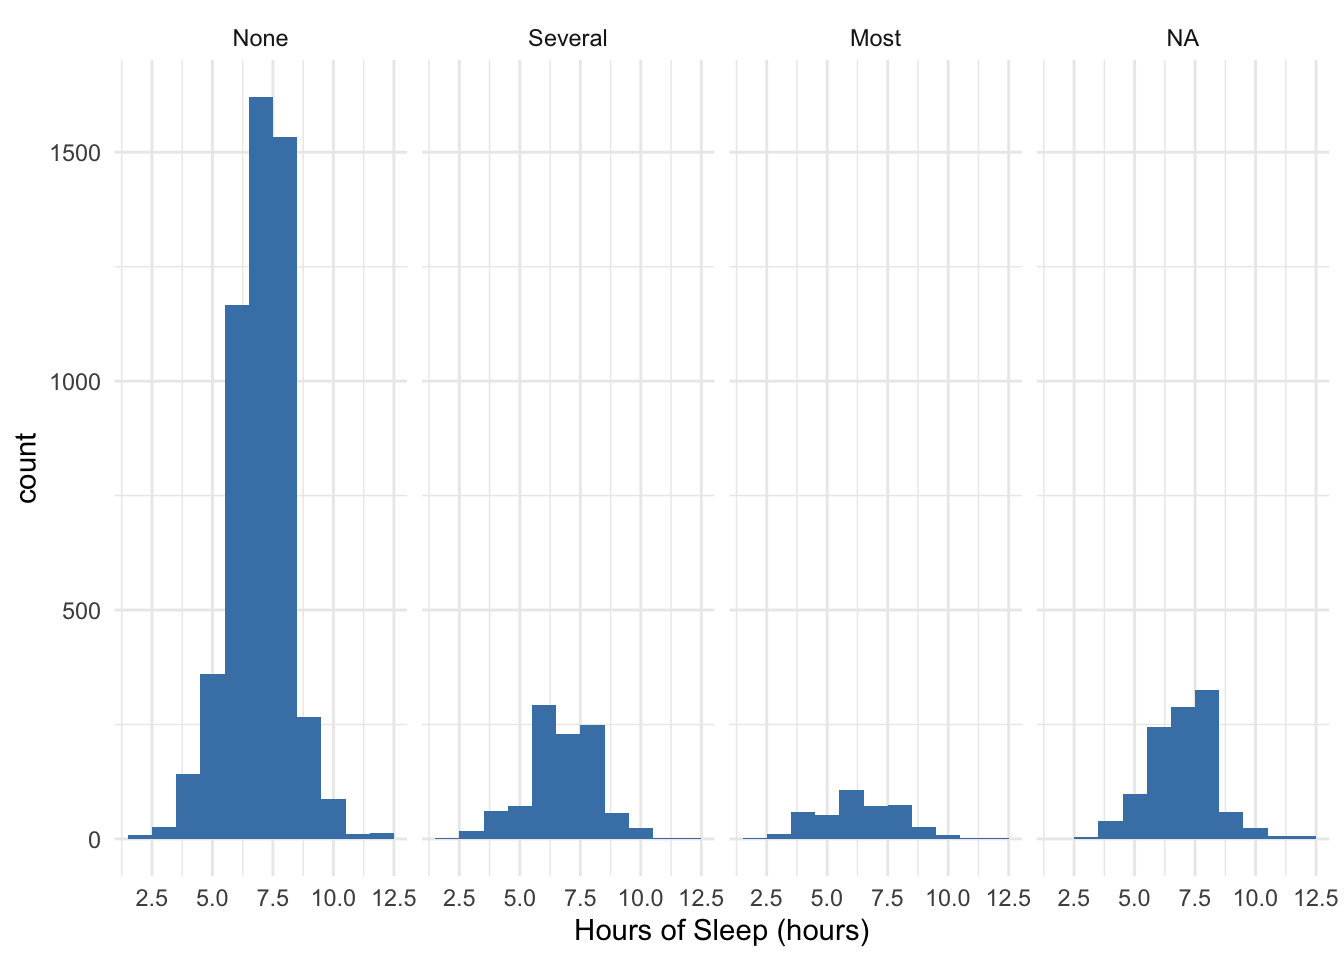
\includegraphics{02-visualization_files/figure-latex/unnamed-chunk-47-1.pdf}

The 0 to 12 labels at the top of each of these panels correspond to the number of babies a woman had.

\begin{reflect}
Do you notice any differences in sleep hour distributions between these
groups?

Note the x and y axes are the same for all of the groups to facilitate
comparison. What is easy to compare and what is hard to compare between
the histograms?
\end{reflect}

\textbf{Does the number of days someone has felt depressed explain the variability in the hours of sleep?}

\begin{Shaded}
\begin{Highlighting}[]
\NormalTok{NHANES }\OperatorTok
\StringTok{    }\KeywordTok{ggplot}\NormalTok{(}\KeywordTok{aes}\NormalTok{(}\DataTypeTok{x =}\NormalTok{ SleepHrsNight)) }\OperatorTok{+}
\StringTok{    }\KeywordTok{geom_histogram}\NormalTok{(}\DataTypeTok{binwidth =} \DecValTok{1}\NormalTok{, }\DataTypeTok{fill =} \StringTok{"steelblue"}\NormalTok{) }\OperatorTok{+}\StringTok{ }
\StringTok{    }\KeywordTok{xlab}\NormalTok{(}\StringTok{'Hours of Sleep (hours)'}\NormalTok{) }\OperatorTok{+}\StringTok{ }
\StringTok{    }\KeywordTok{facet_grid}\NormalTok{(. }\OperatorTok{~}\StringTok{ }\NormalTok{Depressed) }\OperatorTok{+}\StringTok{ }
\StringTok{    }\KeywordTok{theme_minimal}\NormalTok{() }
\end{Highlighting}
\end{Shaded}

\begin{verbatim}
## Warning: Removed 2245 rows containing non-finite values (stat_bin).
\end{verbatim}

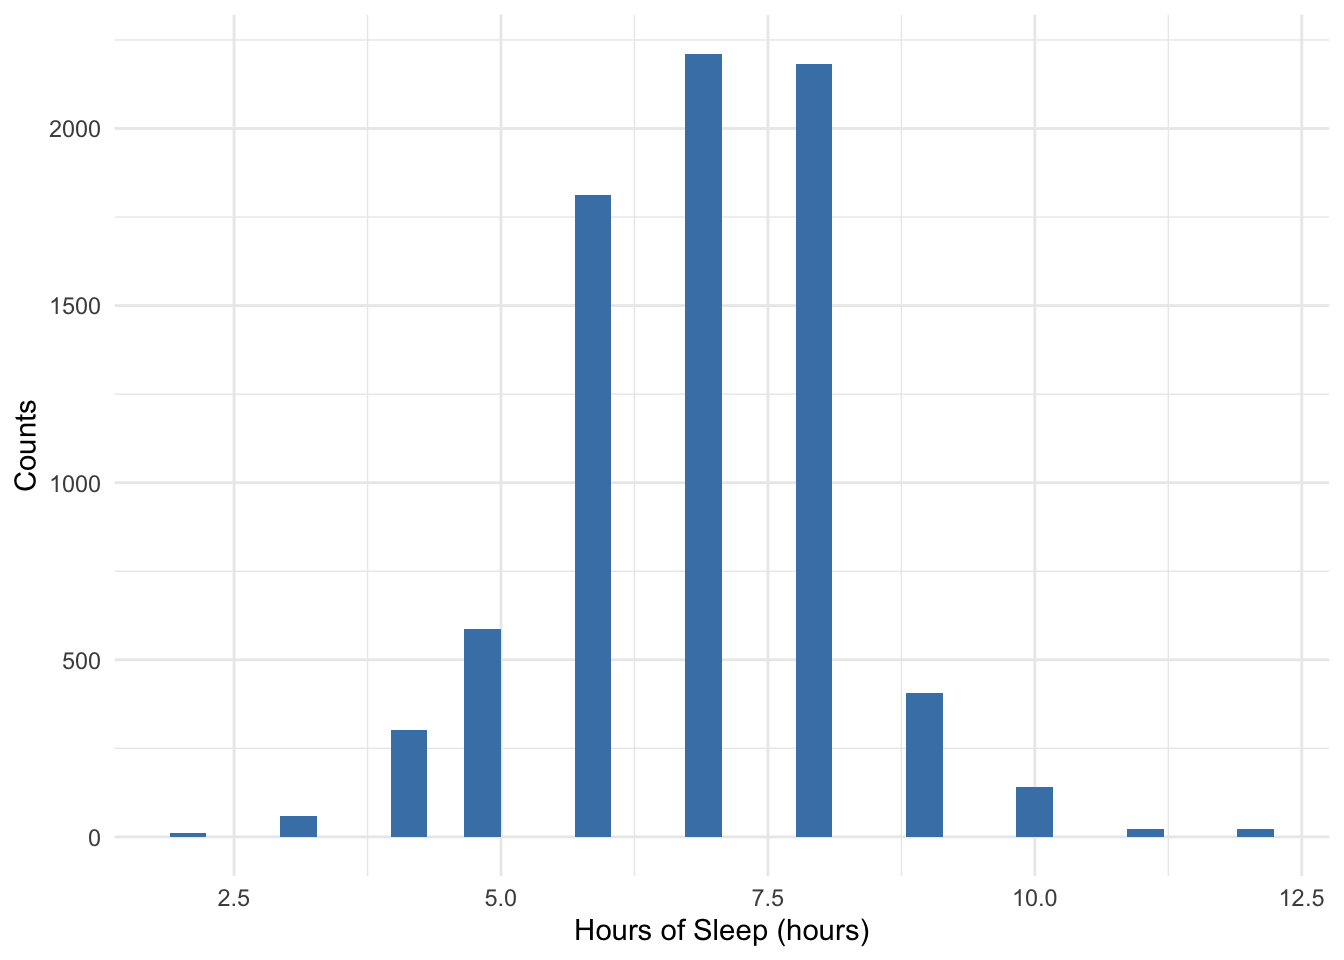
\includegraphics{02-visualization_files/figure-latex/unnamed-chunk-49-1.pdf}

What's the rightmost ``NA'' category? Some individuals in this study did not answer questions about days that they might have felt depressed, but they did report their hours of sleep per night.

\begin{reflect}
What type of biases might be at play here?
\end{reflect}

\hypertarget{multiple-boxplots}{%
\subsection{Multiple Boxplots}\label{multiple-boxplots}}

Let's visualize the same information but with boxplots instead of histograms and see if we can glean any other information.

\begin{Shaded}
\begin{Highlighting}[]
\NormalTok{NHANES }\OperatorTok
\StringTok{    }\KeywordTok{ggplot}\NormalTok{(}\KeywordTok{aes}\NormalTok{(}\DataTypeTok{x =}\NormalTok{ Gender, }\DataTypeTok{y =}\NormalTok{ SleepHrsNight)) }\OperatorTok{+}
\StringTok{    }\KeywordTok{geom_boxplot}\NormalTok{() }\OperatorTok{+}\StringTok{ }
\StringTok{    }\KeywordTok{ylab}\NormalTok{(}\StringTok{'Hours of Sleep (hours)'}\NormalTok{) }\OperatorTok{+}\StringTok{ }
\StringTok{    }\KeywordTok{xlab}\NormalTok{(}\StringTok{'Binary Gender'}\NormalTok{) }\OperatorTok{+}\StringTok{ }
\StringTok{    }\KeywordTok{theme_minimal}\NormalTok{() }
\end{Highlighting}
\end{Shaded}

\begin{verbatim}
## Warning: Removed 2245 rows containing non-finite values (stat_boxplot).
\end{verbatim}

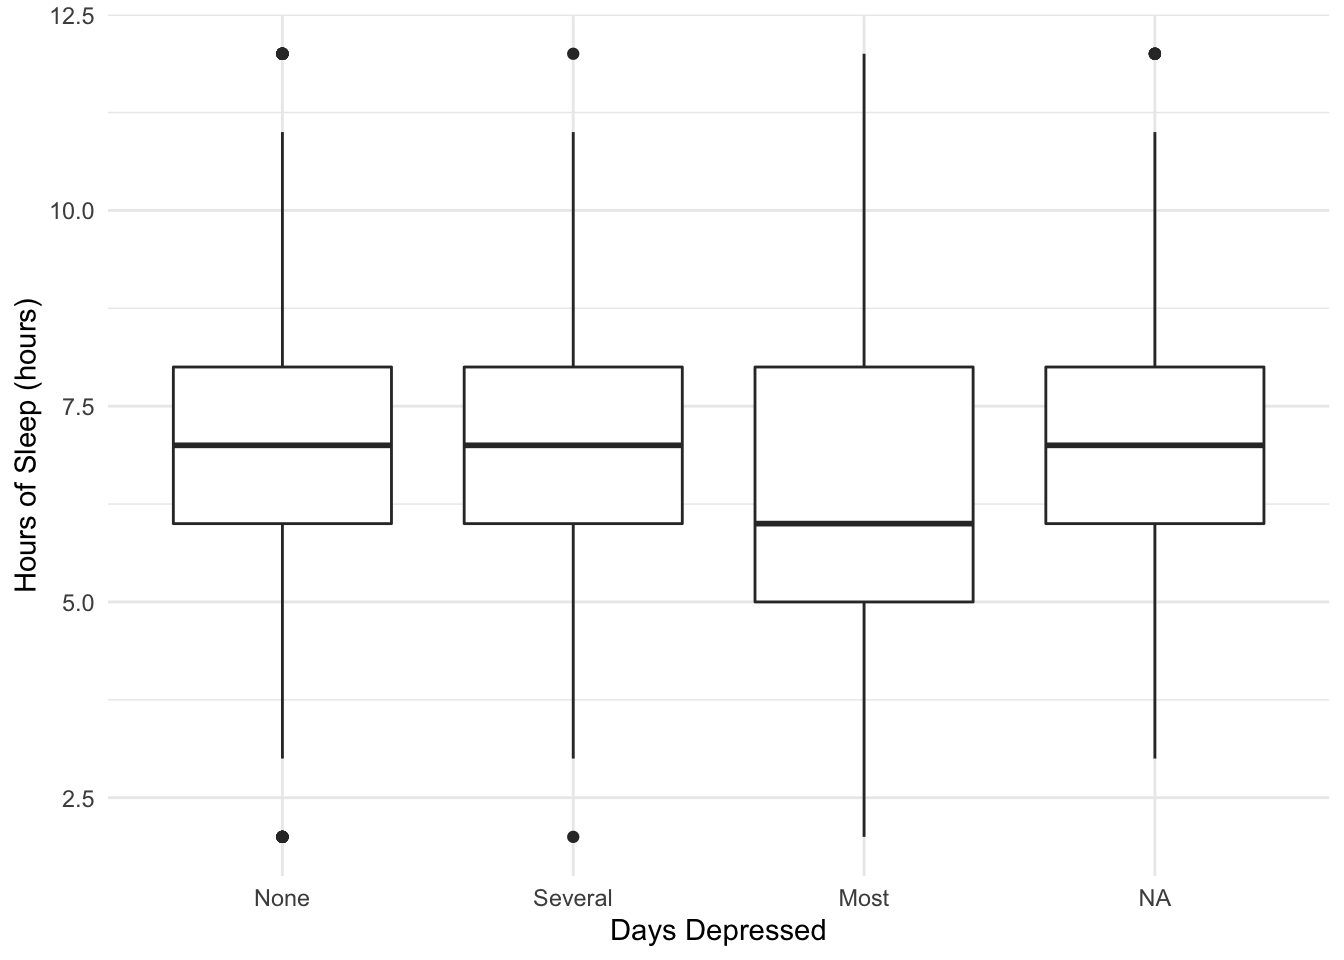
\includegraphics{02-visualization_files/figure-latex/unnamed-chunk-51-1.pdf}

\begin{Shaded}
\begin{Highlighting}[]
\NormalTok{NHANES }\OperatorTok
\StringTok{    }\KeywordTok{ggplot}\NormalTok{(}\KeywordTok{aes}\NormalTok{(}\DataTypeTok{x =} \KeywordTok{factor}\NormalTok{(nBabies), }\DataTypeTok{y =}\NormalTok{ SleepHrsNight)) }\OperatorTok{+}
\StringTok{    }\KeywordTok{geom_boxplot}\NormalTok{() }\OperatorTok{+}\StringTok{ }
\StringTok{    }\KeywordTok{ylab}\NormalTok{(}\StringTok{'Hours of Sleep (hours)'}\NormalTok{) }\OperatorTok{+}\StringTok{ }
\StringTok{    }\KeywordTok{xlab}\NormalTok{(}\StringTok{'Number of Babies'}\NormalTok{) }\OperatorTok{+}\StringTok{ }
\StringTok{    }\KeywordTok{theme_minimal}\NormalTok{() }
\end{Highlighting}
\end{Shaded}

\begin{verbatim}
## Warning: Removed 2245 rows containing non-finite values (stat_boxplot).
\end{verbatim}

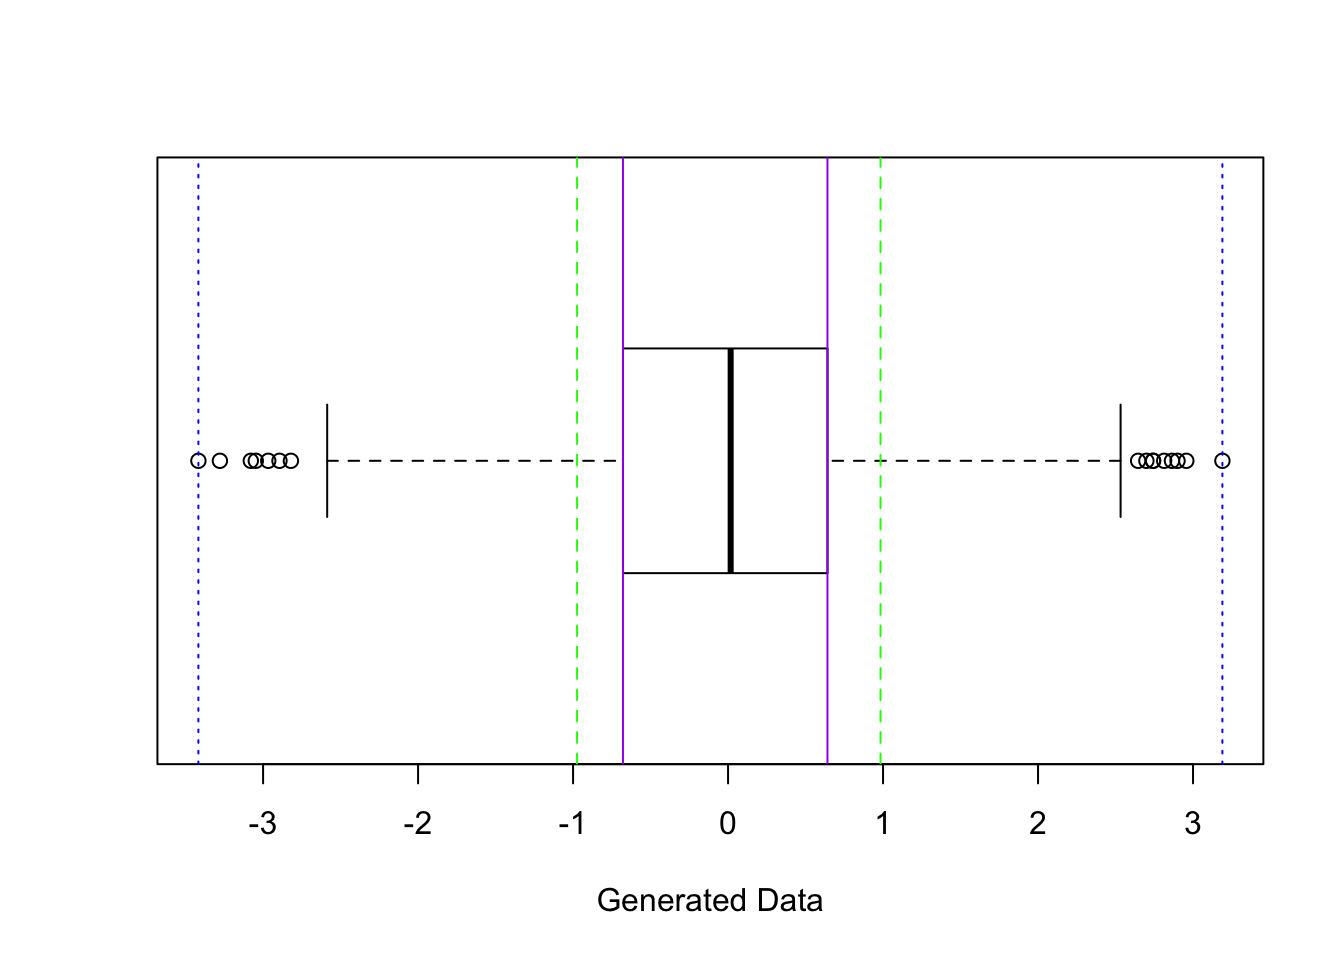
\includegraphics{02-visualization_files/figure-latex/unnamed-chunk-52-1.pdf}

\begin{Shaded}
\begin{Highlighting}[]
\NormalTok{NHANES }\OperatorTok
\StringTok{    }\KeywordTok{ggplot}\NormalTok{(}\KeywordTok{aes}\NormalTok{(}\DataTypeTok{x =} \KeywordTok{factor}\NormalTok{(Depressed), }\DataTypeTok{y =}\NormalTok{ SleepHrsNight)) }\OperatorTok{+}
\StringTok{    }\KeywordTok{geom_boxplot}\NormalTok{() }\OperatorTok{+}\StringTok{ }
\StringTok{    }\KeywordTok{ylab}\NormalTok{(}\StringTok{'Hours of Sleep (hours)'}\NormalTok{) }\OperatorTok{+}\StringTok{ }
\StringTok{    }\KeywordTok{xlab}\NormalTok{(}\StringTok{'Days Depressed'}\NormalTok{) }\OperatorTok{+}\StringTok{ }
\StringTok{    }\KeywordTok{theme_minimal}\NormalTok{() }
\end{Highlighting}
\end{Shaded}

\begin{verbatim}
## Warning: Removed 2245 rows containing non-finite values (stat_boxplot).
\end{verbatim}

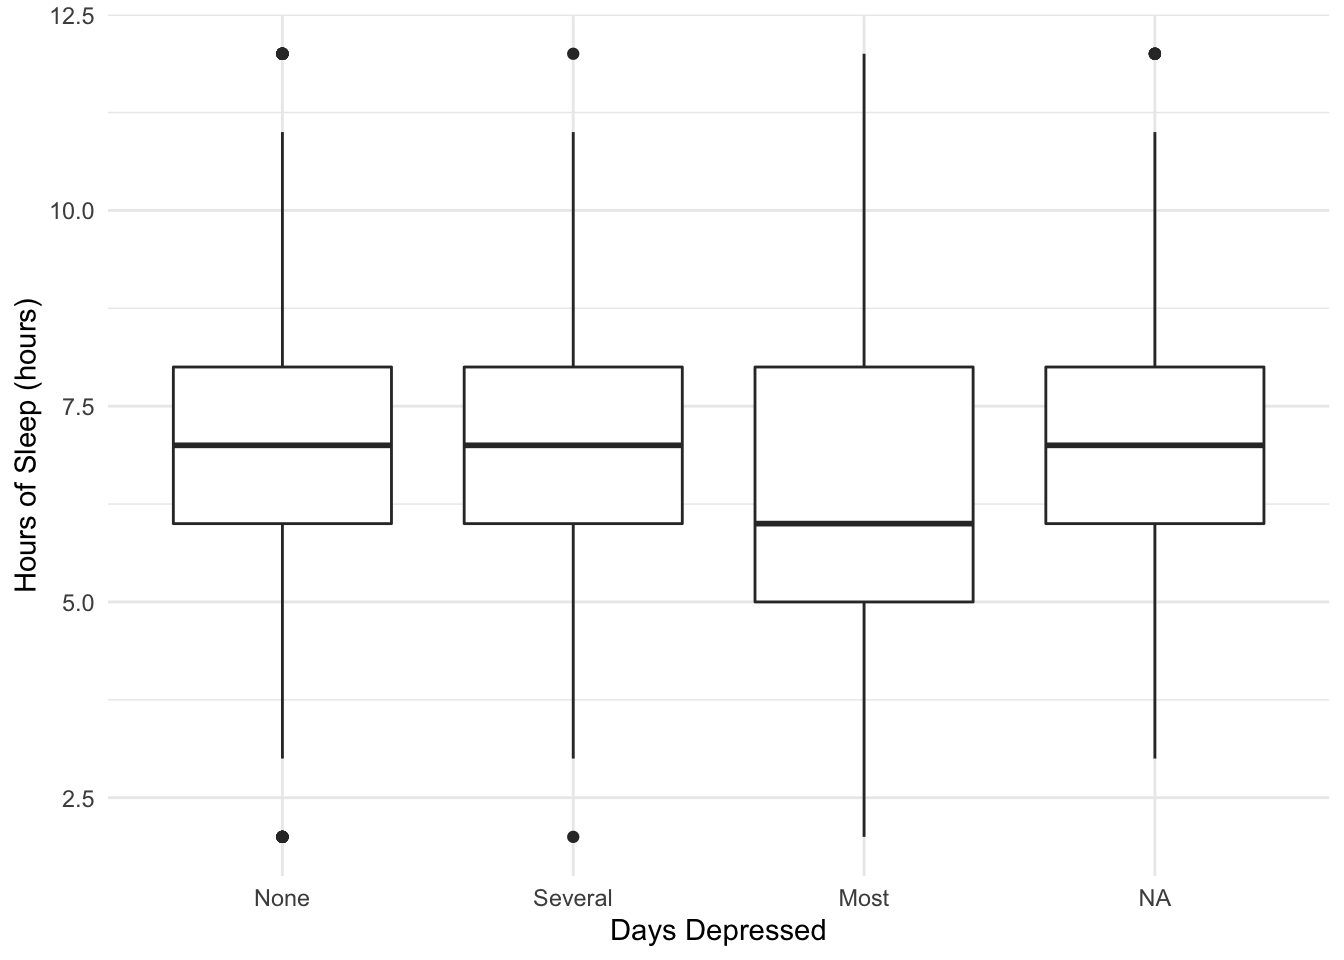
\includegraphics{02-visualization_files/figure-latex/unnamed-chunk-53-1.pdf}

\begin{reflect}
What is easy to compare and what is hard to compare between the
boxplots?

Why might you use multiple boxplots instead of multiple histograms?
\end{reflect}

\hypertarget{is-this-a-real-difference}{%
\subsection{Is this a Real Difference?}\label{is-this-a-real-difference}}

If we notice differences in the the sleep distributions for groups based on self-reported Depression, is it a ``REAL'' difference? That is, is there a difference in the general U.S. population? Remember, we only have a random \emph{sample} of the population. \emph{NHANES is supposed to be a representative sample of the U.S. population collected using a probability sampling procedure.}

What if there were no ``REAL'' difference? Then the Depressed group labels wouldn't be related to the hours of sleep.

\textbf{Investigation Plan:}

\begin{enumerate}
\def\labelenumi{\arabic{enumi}.}
\tightlist
\item
  Take all of the observed data on the hours of sleep and randomly shuffle them into new groups (of the same sizes as before). This breaks any associations between the Depressed group labels and the reported hours of sleep.
\item
  Calculate the difference in mean hours of sleep between the groups. Record it.
\item
  Repeat steps 1 and 2 many times (say 1000 times).
\item
  Look at the differences based on random shuffles \& compare to the observed difference.
\end{enumerate}

\begin{Shaded}
\begin{Highlighting}[]
\KeywordTok{library}\NormalTok{(mosaic) }
\end{Highlighting}
\end{Shaded}

\begin{verbatim}
## Loading required package: lattice
\end{verbatim}

\begin{verbatim}
## Loading required package: ggformula
\end{verbatim}

\begin{verbatim}
## Loading required package: ggstance
\end{verbatim}

\begin{verbatim}
## 
## Attaching package: 'ggstance'
\end{verbatim}

\begin{verbatim}
## The following objects are masked from 'package:ggplot2':
## 
##     geom_errorbarh, GeomErrorbarh
\end{verbatim}

\begin{verbatim}
## 
## New to ggformula?  Try the tutorials: 
## 	learnr::run_tutorial("introduction", package = "ggformula")
## 	learnr::run_tutorial("refining", package = "ggformula")
\end{verbatim}

\begin{verbatim}
## Loading required package: Matrix
\end{verbatim}

\begin{verbatim}
## Registered S3 method overwritten by 'mosaic':
##   method                           from   
##   fortify.SpatialPolygonsDataFrame ggplot2
\end{verbatim}

\begin{verbatim}
## 
## The 'mosaic' package masks several functions from core packages in order to add 
## additional features.  The original behavior of these functions should not be affected by this.
## 
## Note: If you use the Matrix package, be sure to load it BEFORE loading mosaic.
## 
## Have you tried the ggformula package for your plots?
\end{verbatim}

\begin{verbatim}
## 
## Attaching package: 'mosaic'
\end{verbatim}

\begin{verbatim}
## The following object is masked from 'package:Matrix':
## 
##     mean
\end{verbatim}

\begin{verbatim}
## The following object is masked from 'package:ggplot2':
## 
##     stat
\end{verbatim}

\begin{verbatim}
## The following objects are masked from 'package:dplyr':
## 
##     count, do, tally
\end{verbatim}

\begin{verbatim}
## The following objects are masked from 'package:stats':
## 
##     binom.test, cor, cor.test, cov, fivenum, IQR, median, prop.test,
##     quantile, sd, t.test, var
\end{verbatim}

\begin{verbatim}
## The following objects are masked from 'package:base':
## 
##     max, mean, min, prod, range, sample, sum
\end{verbatim}

\begin{Shaded}
\begin{Highlighting}[]
\NormalTok{NHANES <-}\StringTok{ }\NormalTok{NHANES }\OperatorTok
\StringTok{  }\KeywordTok{mutate}\NormalTok{(}\DataTypeTok{DepressedMost =}\NormalTok{ (Depressed }\OperatorTok{==}\StringTok{ 'Most'}\NormalTok{)) }\CommentTok{#TRUE or FALSE (converted Depressed to a 2 category variable)}

\NormalTok{obsdiff <-}\StringTok{ }\KeywordTok{data.frame}\NormalTok{(}\DataTypeTok{d =} \KeywordTok{diff}\NormalTok{(}\KeywordTok{mean}\NormalTok{(SleepHrsNight }\OperatorTok{~}\StringTok{ }\NormalTok{DepressedMost, }\DataTypeTok{data =}\NormalTok{ NHANES, }\DataTypeTok{na.rm =} \OtherTok{TRUE}\NormalTok{)))}

\NormalTok{sim <-}\StringTok{ }\KeywordTok{do}\NormalTok{(}\DecValTok{1000}\NormalTok{)}\OperatorTok{*}\KeywordTok{diff}\NormalTok{(}\KeywordTok{mean}\NormalTok{(SleepHrsNight }\OperatorTok{~}\StringTok{ }\KeywordTok{shuffle}\NormalTok{(DepressedMost), }\DataTypeTok{data =}\NormalTok{ NHANES, }\DataTypeTok{na.rm =} \OtherTok{TRUE}\NormalTok{)) }\CommentTok{#Randomly shuffle the DepressedMost labels (assuming no real difference in sleep, depressed feelings shouldn't impact sleep)}
\end{Highlighting}
\end{Shaded}

Below, we have a histogram of 1000 values calculated by randomly shuffling individuals in the sample into two groups (assuming no relationship between depression and sleep) and then finding the difference in the mean amount of sleep. The red vertical line showed the observed difference in mean amount of sleep in the data.

\begin{Shaded}
\begin{Highlighting}[]
\NormalTok{sim }\OperatorTok
\StringTok{  }\KeywordTok{ggplot}\NormalTok{(}\KeywordTok{aes}\NormalTok{(}\DataTypeTok{x =}\NormalTok{ TRUE.)) }\OperatorTok{+}\StringTok{ }
\StringTok{  }\KeywordTok{geom_histogram}\NormalTok{(}\DataTypeTok{fill =} \StringTok{'steelblue'}\NormalTok{) }\OperatorTok{+}
\StringTok{  }\KeywordTok{geom_vline}\NormalTok{(}\KeywordTok{aes}\NormalTok{(}\DataTypeTok{xintercept =}\NormalTok{ d), obsdiff, }\DataTypeTok{color =} \StringTok{'red'}\NormalTok{) }\OperatorTok{+}\StringTok{ }
\StringTok{  }\KeywordTok{xlab}\NormalTok{(}\StringTok{'Difference in Mean Hours of Sleep'}\NormalTok{) }\OperatorTok{+}\StringTok{ }
\StringTok{  }\KeywordTok{ylab}\NormalTok{(}\StringTok{'Counts'}\NormalTok{) }\OperatorTok{+}\StringTok{ }
\StringTok{  }\KeywordTok{theme_minimal}\NormalTok{() }
\end{Highlighting}
\end{Shaded}

\begin{verbatim}
## `stat_bin()` using `bins = 30`. Pick better value with `binwidth`.
\end{verbatim}

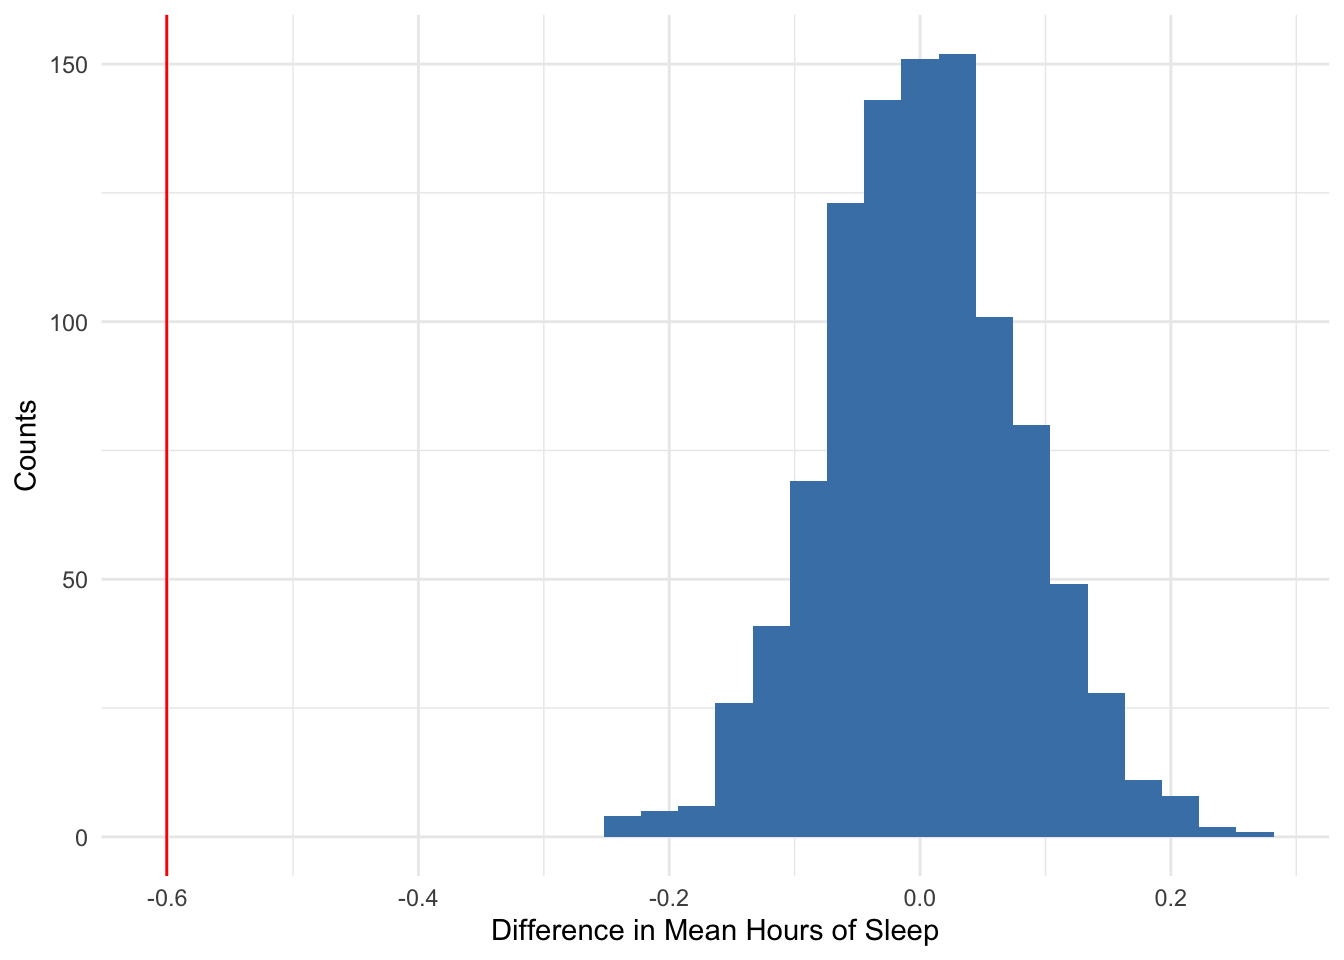
\includegraphics{02-visualization_files/figure-latex/unnamed-chunk-56-1.pdf}

\begin{reflect}
The observed difference in mean hours of sleep (red line) is quite far
from the distribution of differences that results when we break the
association between depression status and sleep hours (through
randomized shuffling of group labels). Thus, it is unlikely to get a
difference that large if there were no relationhip.

What do you think this indicates? How might you use this as evidence for
or against a ``real'' population difference?
\end{reflect}

\hypertarget{two-quantitative-variables}{%
\section{Two Quantitative Variables}\label{two-quantitative-variables}}

To discuss two quantitative variables, let's switch to new data set and consider a thought experiment.

Imagine that you are an entrepreneur selling button-down dress shirts. Clothing sizing are quite variable across clothing brands, so we are going to use our own data to come up with appropriate sizes for our customers. Two of the key measurements that we will use are the neck size in centimeters and chest size in centimeters of a customer. There are other variables in the data set, but let's focus on these two for the moment.

\hypertarget{scatterplot}{%
\subsection{Scatterplot}\label{scatterplot}}

When you have two quantitative variables, a \textbf{scatterplot} is the main appropriate graphical display of the relationship. Each point represents the neck and chest size of one customer.

\begin{Shaded}
\begin{Highlighting}[]
\NormalTok{body <-}\StringTok{ }\KeywordTok{read.delim}\NormalTok{(}\StringTok{"Data/bodyfat.txt"}\NormalTok{)}

\NormalTok{body }\OperatorTok
\StringTok{    }\KeywordTok{ggplot}\NormalTok{(}\KeywordTok{aes}\NormalTok{(}\DataTypeTok{x =}\NormalTok{ Neck, }\DataTypeTok{y =}\NormalTok{ Chest)) }\OperatorTok{+}
\StringTok{    }\KeywordTok{geom_point}\NormalTok{(}\DataTypeTok{color =} \StringTok{'steelblue'}\NormalTok{) }\OperatorTok{+}\StringTok{ }
\StringTok{    }\KeywordTok{xlab}\NormalTok{(}\StringTok{'Neck size (cm)'}\NormalTok{) }\OperatorTok{+}\StringTok{ }
\StringTok{    }\KeywordTok{ylab}\NormalTok{(}\StringTok{'Chest size (cm)'}\NormalTok{) }\OperatorTok{+}
\StringTok{    }\KeywordTok{theme_minimal}\NormalTok{()}
\end{Highlighting}
\end{Shaded}

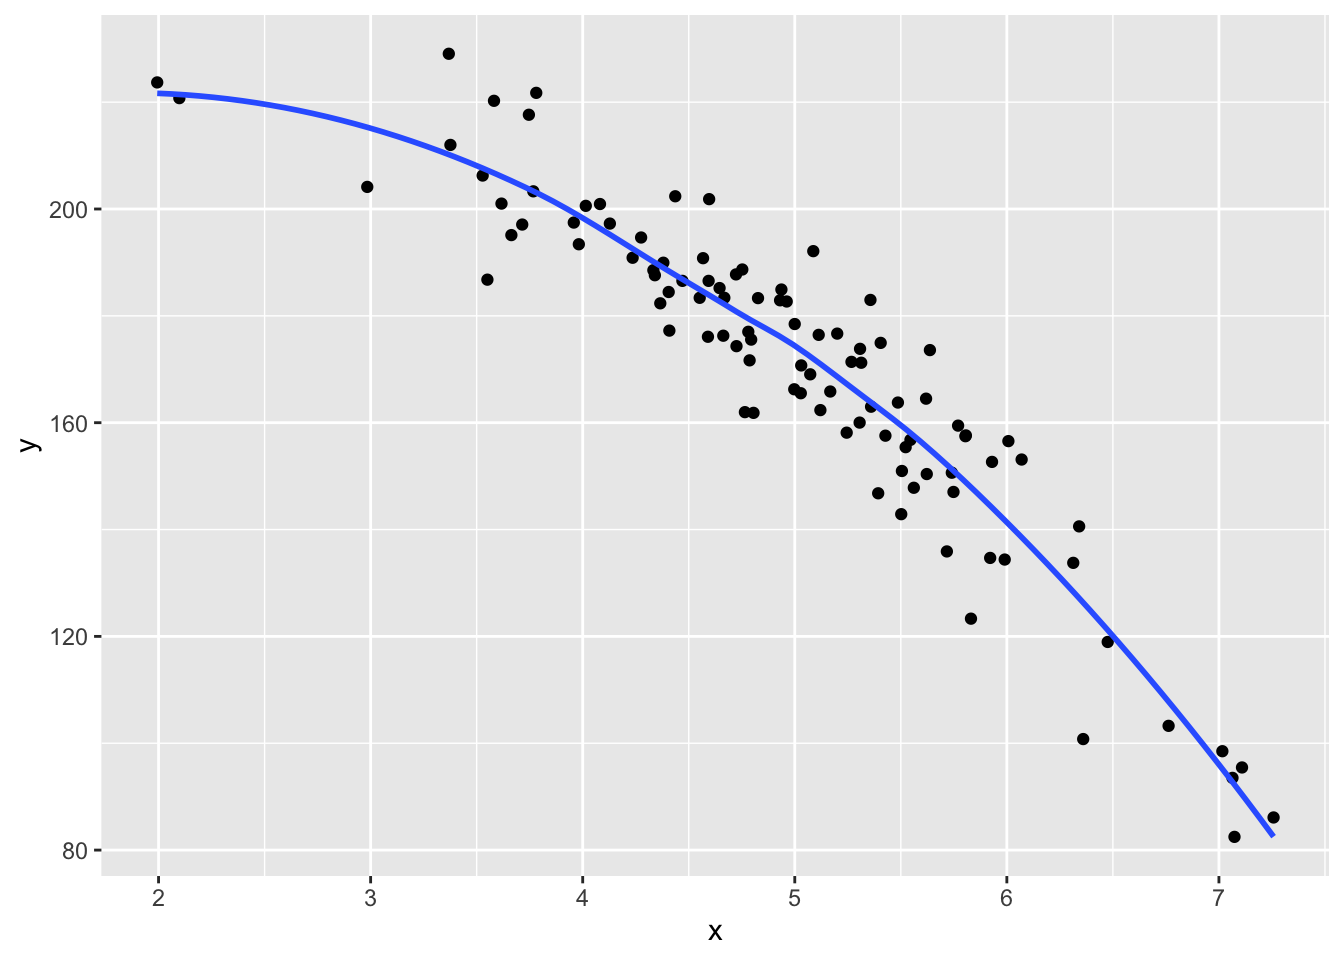
\includegraphics{02-visualization_files/figure-latex/unnamed-chunk-58-1.pdf}

What do you notice about:

\begin{enumerate}
\def\labelenumi{\arabic{enumi}.}
\tightlist
\item
  \textbf{Direction} of relationship (positive, negative, or neutral)
\item
  \textbf{Form} of relationship (linear, curved, none, or other)
\item
  \textbf{Strength} of relationship (compactness around the average relationship)
\item
  \textbf{Unusual} features (outliers, differences in variability in \(y\) variable across different values of \(x\) variable)
\end{enumerate}

\begin{reflect}
How might you use this information to determine shirt sizes for your new
business venture? Come up with a few ways you could define sizes such as
small, medium, large, extra large, etc.
\end{reflect}

Suppose instead of \emph{Chest} in inches and \emph{Neck size} in cm, we plotted \emph{Chest} in inches and \emph{Neck size} in inches.

\textbf{Does the strength of the relationship change after transformation?}

Look at the plot in inches below. Does this plot look the same as the centimeters plot?

\begin{Shaded}
\begin{Highlighting}[]
\NormalTok{body }\OperatorTok
\StringTok{  }\KeywordTok{ggplot}\NormalTok{(}\KeywordTok{aes}\NormalTok{(}\DataTypeTok{x =}\NormalTok{ Neck}\OperatorTok{/}\FloatTok{2.54}\NormalTok{, }\DataTypeTok{y =}\NormalTok{ Chest}\OperatorTok{/}\FloatTok{2.54}\NormalTok{)) }\OperatorTok{+}
\StringTok{  }\KeywordTok{geom_point}\NormalTok{(}\DataTypeTok{color =} \StringTok{'steelblue'}\NormalTok{) }\OperatorTok{+}\StringTok{ }
\StringTok{  }\KeywordTok{xlab}\NormalTok{(}\StringTok{'Neck size (in)'}\NormalTok{) }\OperatorTok{+}\StringTok{ }
\StringTok{  }\KeywordTok{ylab}\NormalTok{(}\StringTok{'Chest size (in)'}\NormalTok{) }\OperatorTok{+}
\StringTok{  }\KeywordTok{theme_minimal}\NormalTok{()}
\end{Highlighting}
\end{Shaded}

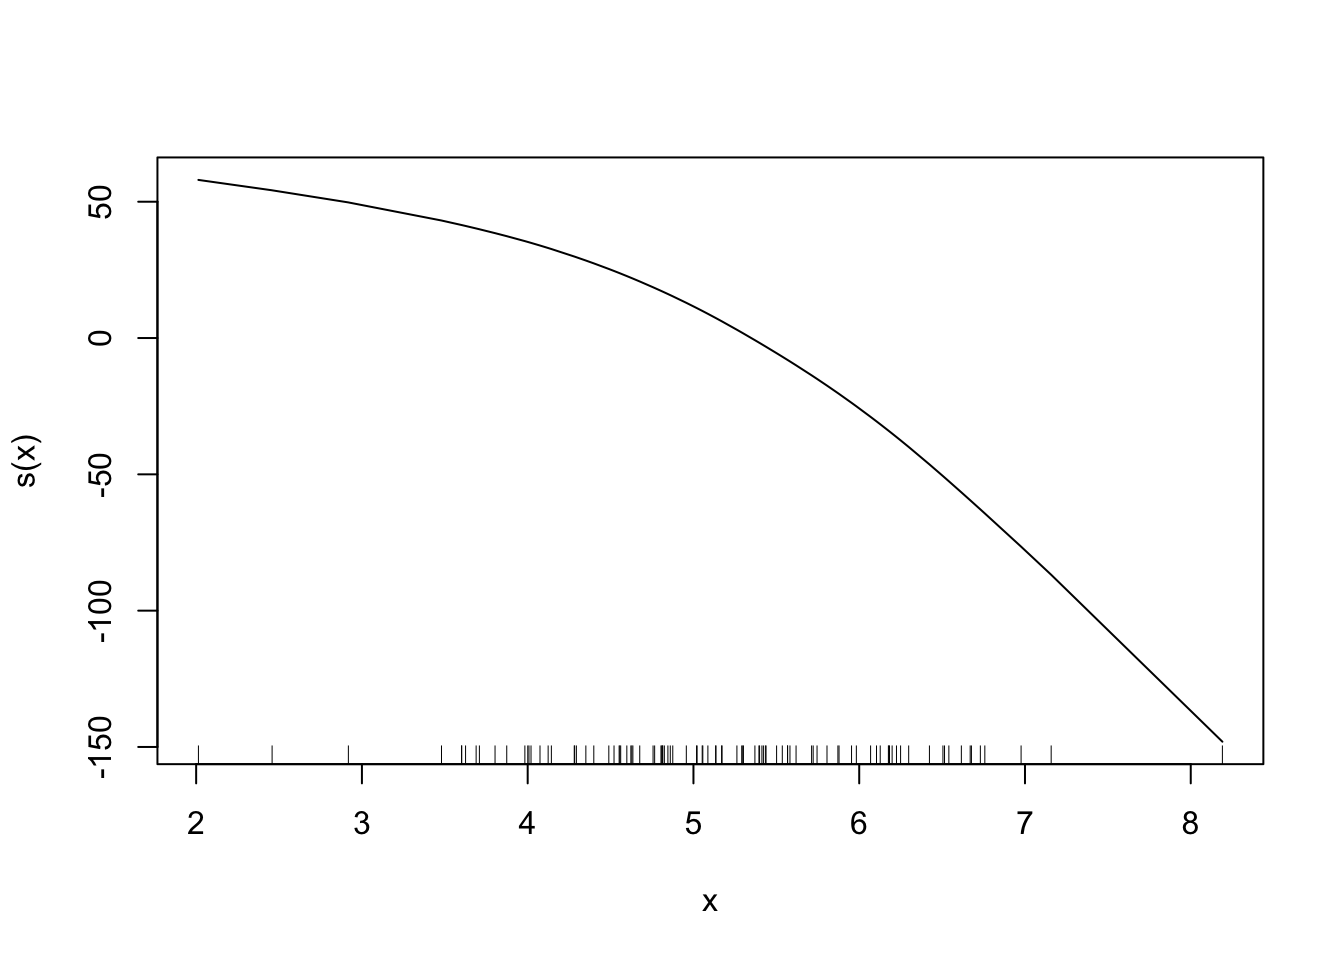
\includegraphics{02-visualization_files/figure-latex/unnamed-chunk-60-1.pdf}

You should see that the x-axes changed but the overall shape of the plot stayed the same. Thus, the strength of the relationship was not affected by tranforming neck size from centimeters to inches (by dividing by 2.54).

\hypertarget{correlation-coefficient}{%
\subsection{Correlation Coefficient}\label{correlation-coefficient}}

Since \textbf{shifting} (adding or subtracting) and \textbf{scaling} (multiplying or dividing) make no difference in the strength of the relationship, let's standardize both variables into z-scores (recall z-scores from Section \ref{intro-zscore}).

Below we plot Neck and Chest sizes after changing them to z-scores with the function \texttt{scale()} and we add some color:

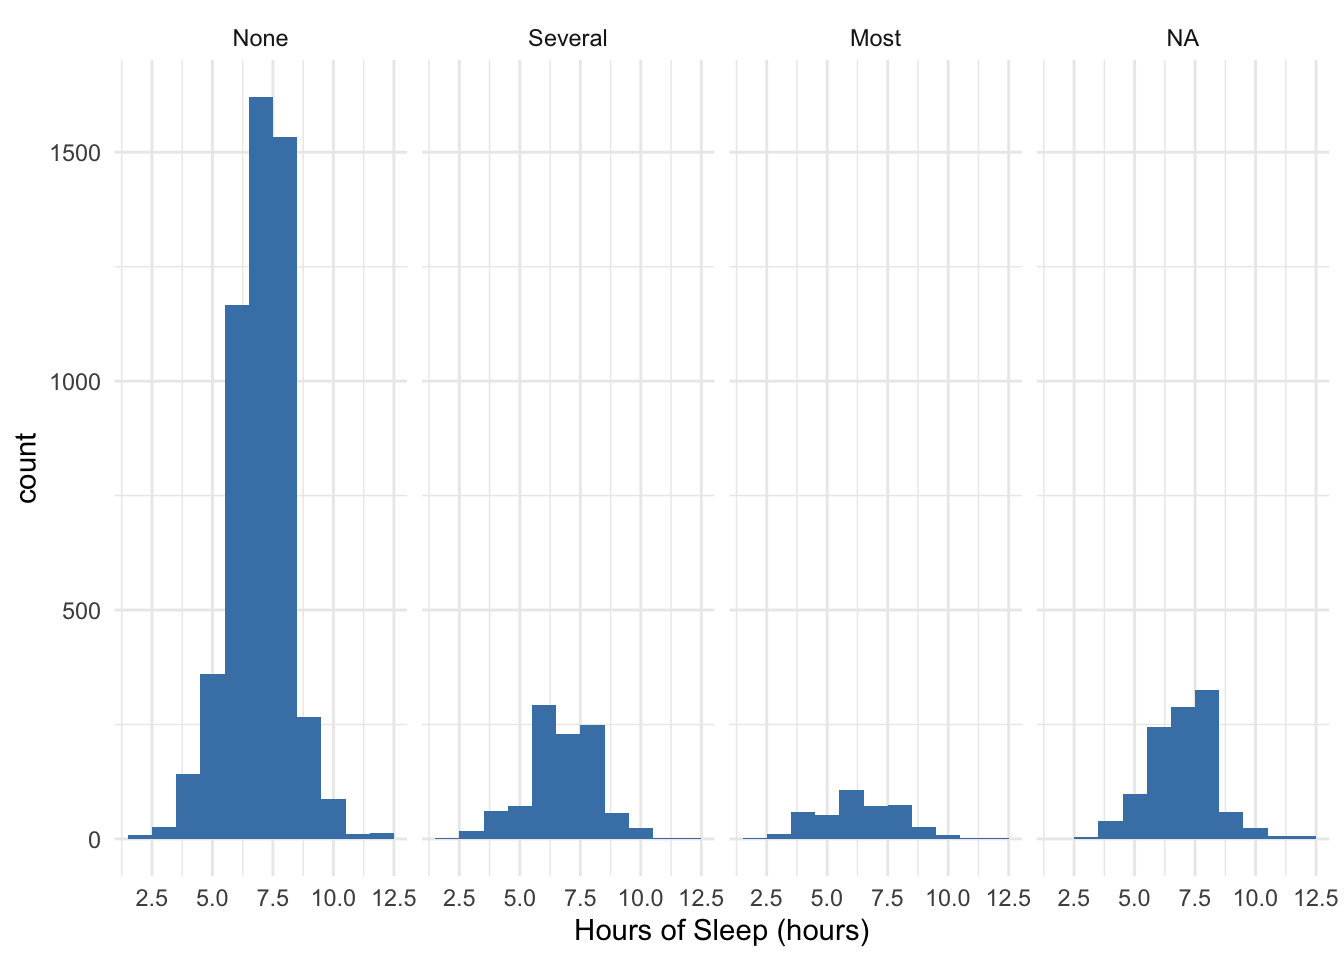
\includegraphics{02-visualization_files/figure-latex/unnamed-chunk-61-1.pdf}

The blue points in the upper right (Quadrant 1) and lower left (Quadrant 3) quadrants are either both positive or both negative in their z-score values. This means that those individuals are above average in both Neck Size and Chest Size (upper right), or they are below average in both Neck Size and Chest Size (lower left). If we multiply the z-scores of the Neck and Chest values for the blue points, we will get a positive value.

The red points in the upper left (Quadrant 2) and lower right (Quadrant 4) quadrants are positive in one and negative in the other. This means that those individuals are either above average in Neck Size but below average in Chest Size (lower right) or they are below average in Neck Size and above average in Chest Size (upper left). If we multiply the z-scores of the Neck and Chest values for the red points, we will get a negative value.

\begin{reflect}
If we were to have a weaker positive relationship, how would this plot
change?

If we were to have a stronger positive relationship, how would this plot
change?

If we were to have a negative relationship, how would this plot change?
\end{reflect}

We want one number to represent \textbf{strength} and \textbf{direction} of a linear relationship.

\begin{itemize}
\tightlist
\item
  Points in Quadrants 1 and 3 (blue) have the z-scores of the \textbf{same sign}.
\item
  Points in Quadrants 2 and 4 (red) have z-scores of the \textbf{opposite sign}.
\end{itemize}

\textbf{What if we took the product of the \(z\)-scores for \(x\) and \(y\) variables?}

Situation 1: An individual far above the means in both the \(x\) and \(y\) variables or far below the means in both the \(x\) and \(y\) variables has a very large, positive product of z-scores.

Situation 2: An individual far above the mean in \(x\) and far below the mean in \(y\) has a very large, negative product of z-scores. (The same goes for low \(x\) and high \(y\).)

The (almost) \emph{average} of products of the \(z\)-scores is the \textbf{correlation coefficient},

\[ r_{x,y} = \frac{\sum z_x z_y}{n-1} \]

We notate the correlation coefficient between variables \(x\) and \(y\) as \(r_{x,y}\).

Some observations:

\begin{itemize}
\tightlist
\item
  If most of our data points follow Situation 1, the correlation coefficient is an average of mostly large positive values. Thus the correlation coefficient will be large and positive.
\item
  If most of our data points follow Situation 2, the correlation coefficient is an average of mostly large negative values. Thus the correlation coefficient will be large and negative.
\item
  If about an equal number of data points follow Situation 1 and Situation 2, we will be balancing positive and negative numbers, which results in a value close to zero. Thus, the correlation coefficient will be close to zero.
\end{itemize}

\textbf{Which points contribute the most to this average?}

Let's look at the correlation for the entire sample first. Then let's calculate the correlation for individuals around the mean Neck size.

\begin{Shaded}
\begin{Highlighting}[]
\NormalTok{body }\OperatorTok
\StringTok{  }\KeywordTok{summarize}\NormalTok{(}\KeywordTok{cor}\NormalTok{(Neck, Chest)) }\CommentTok{# All data points used in calculation}
\end{Highlighting}
\end{Shaded}

\begin{verbatim}
##   cor(Neck, Chest)
## 1        0.7688109
\end{verbatim}

\begin{Shaded}
\begin{Highlighting}[]
\NormalTok{body }\OperatorTok
\StringTok{    }\KeywordTok{filter}\NormalTok{(Neck }\OperatorTok{>}\StringTok{ }\DecValTok{35} \OperatorTok{&}\StringTok{ }\NormalTok{Neck }\OperatorTok{<}\StringTok{ }\DecValTok{40}\NormalTok{) }\OperatorTok\StringTok{ }\CommentTok{# Keep individuals with Neck size between 35cm and 40cm}
\StringTok{      }\KeywordTok{summarize}\NormalTok{(}\KeywordTok{cor}\NormalTok{(Neck, Chest)) }\CommentTok{# Only middle subset of data points used in calculation}
\end{Highlighting}
\end{Shaded}

\begin{verbatim}
##   cor(Neck, Chest)
## 1        0.5658835
\end{verbatim}

The value is much larger and more positive when all data points are used. The points that are far from the means of x and y have a larger product of z-scores and thus increase the correlation coefficient value.

\hypertarget{properties}{%
\subsection{Properties}\label{properties}}

\begin{itemize}
\item
  \(-1 \leq r \leq 1\) (due to the \href{https://en.wikipedia.org/wiki/Cauchy\%E2\%80\%93Schwarz_inequality}{Cauchy-Schwarz Inequality} for those are inclined)
\item
  The sign of \(r\) goes with the direction of the relationship.
\item
  \(r_{x,y} = r_{y,x}\), it doesn't matter which variable is \(x\) and which is \(y\).
\item
  \(r_{ax+b, cy+d} = r_{x,y}\), linear change of scale doesn't affect \(r\). Why?
\item
  \(r\) measures strength of \emph{linear} relationship (not a curved relationship).
\item
  One outlier can completely change \(r\).
\end{itemize}

Let's look at a few scatterplot examples and the corresponding correlation.

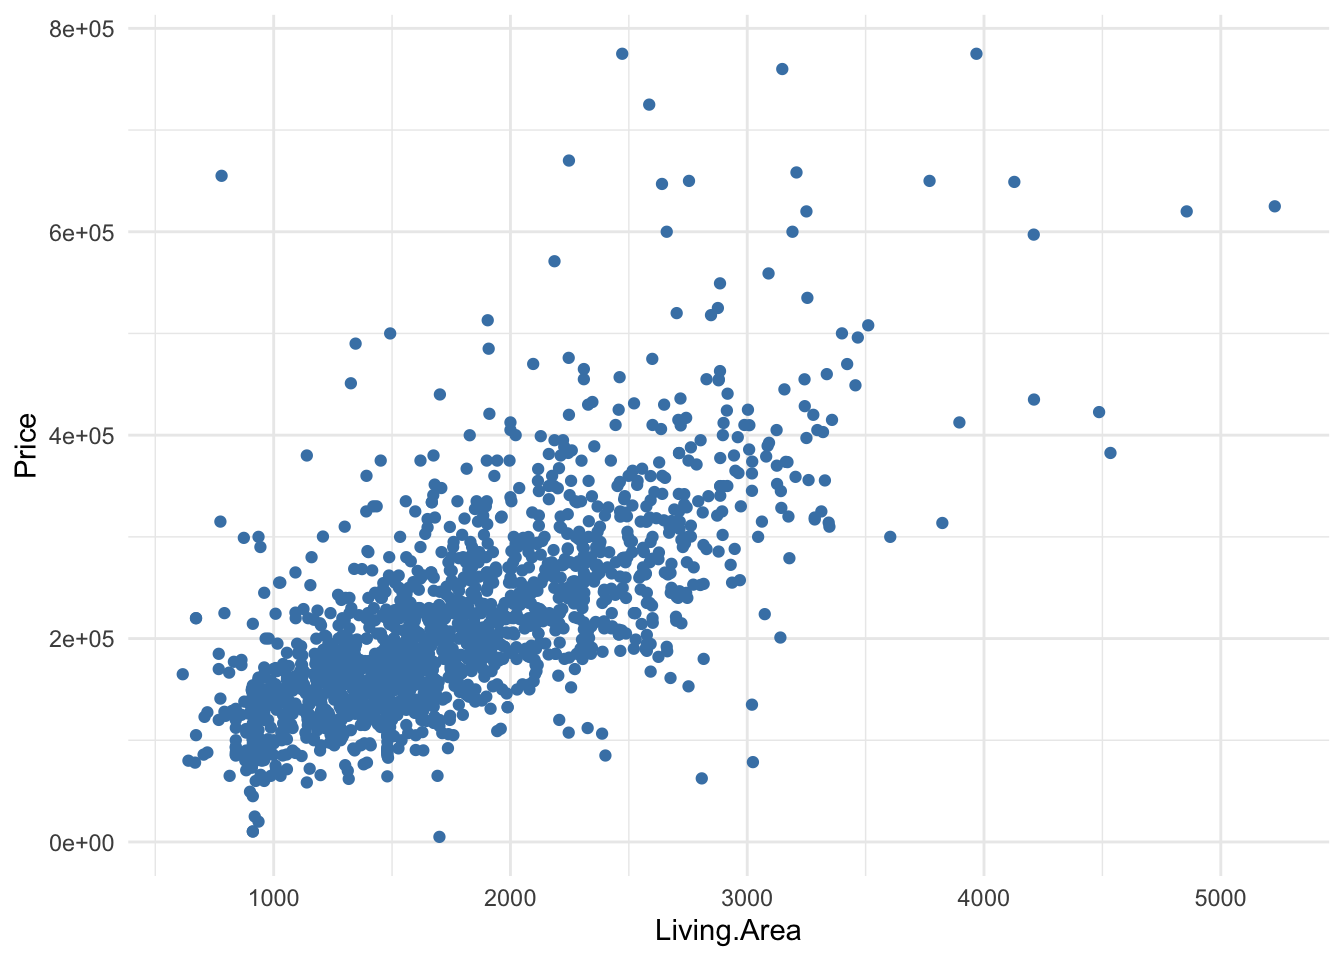
\includegraphics{02-visualization_files/figure-latex/unnamed-chunk-65-1.pdf} 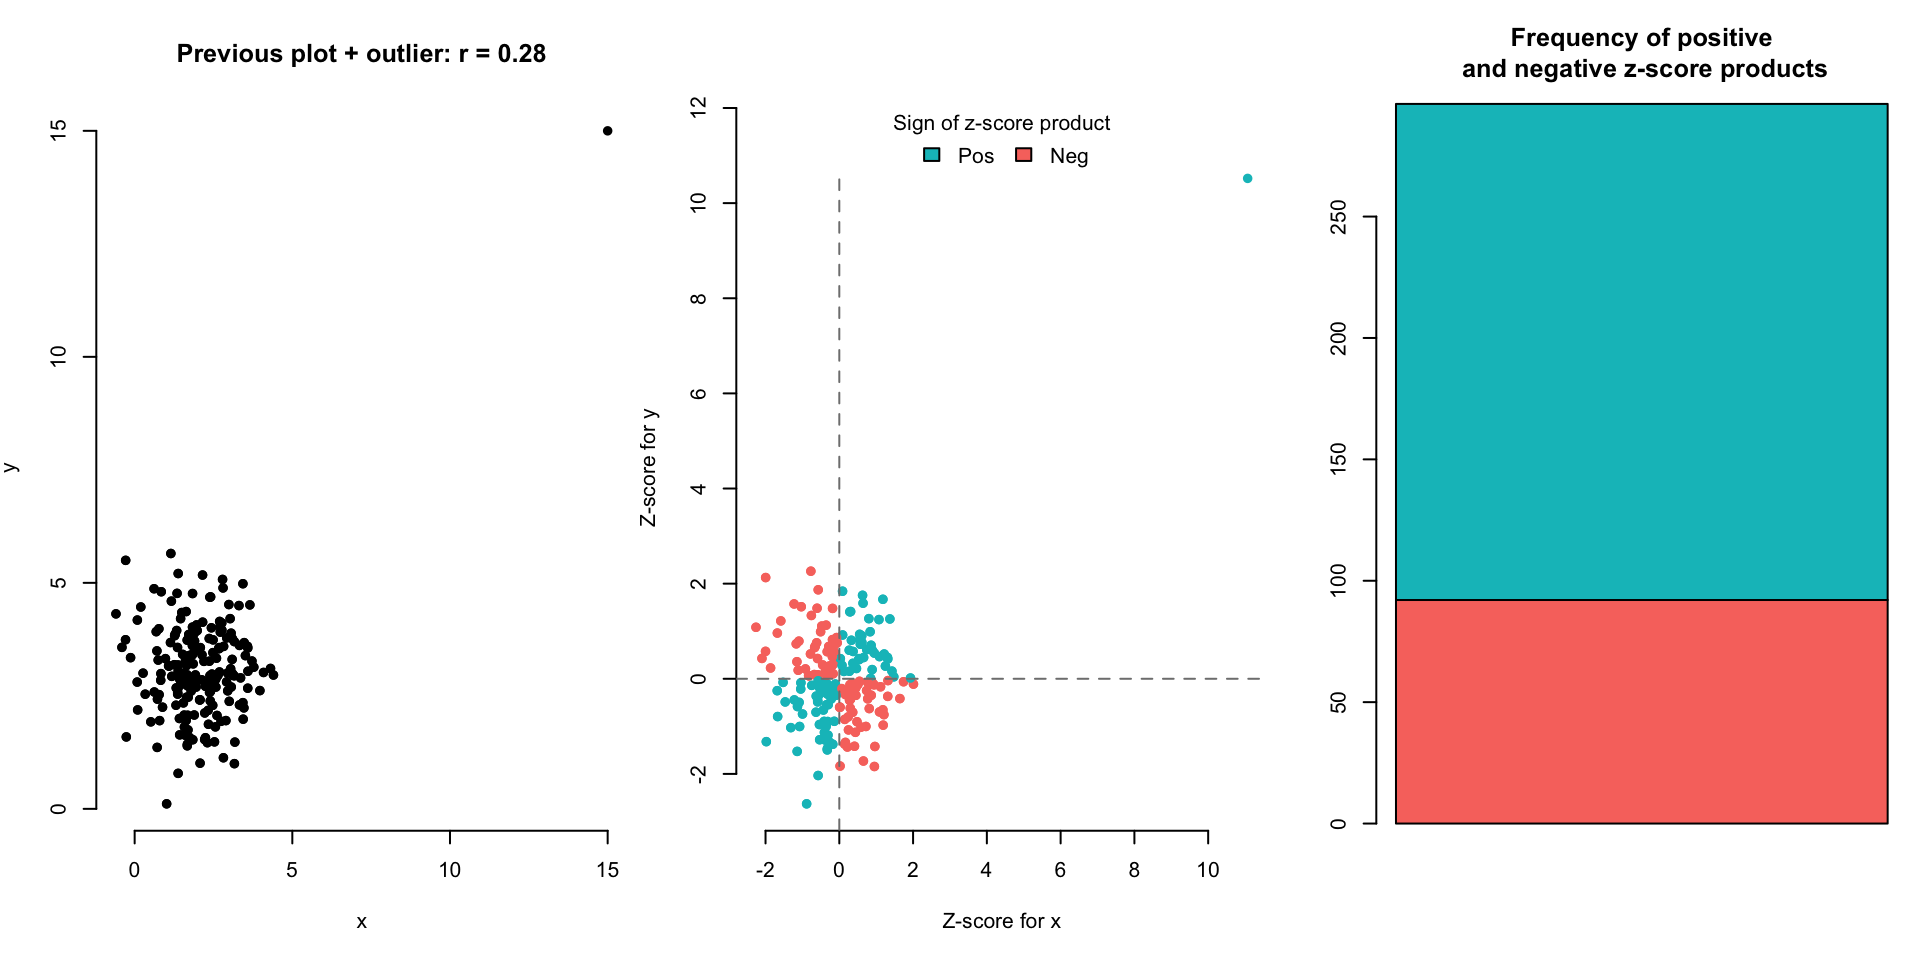
\includegraphics{02-visualization_files/figure-latex/unnamed-chunk-65-2.pdf} 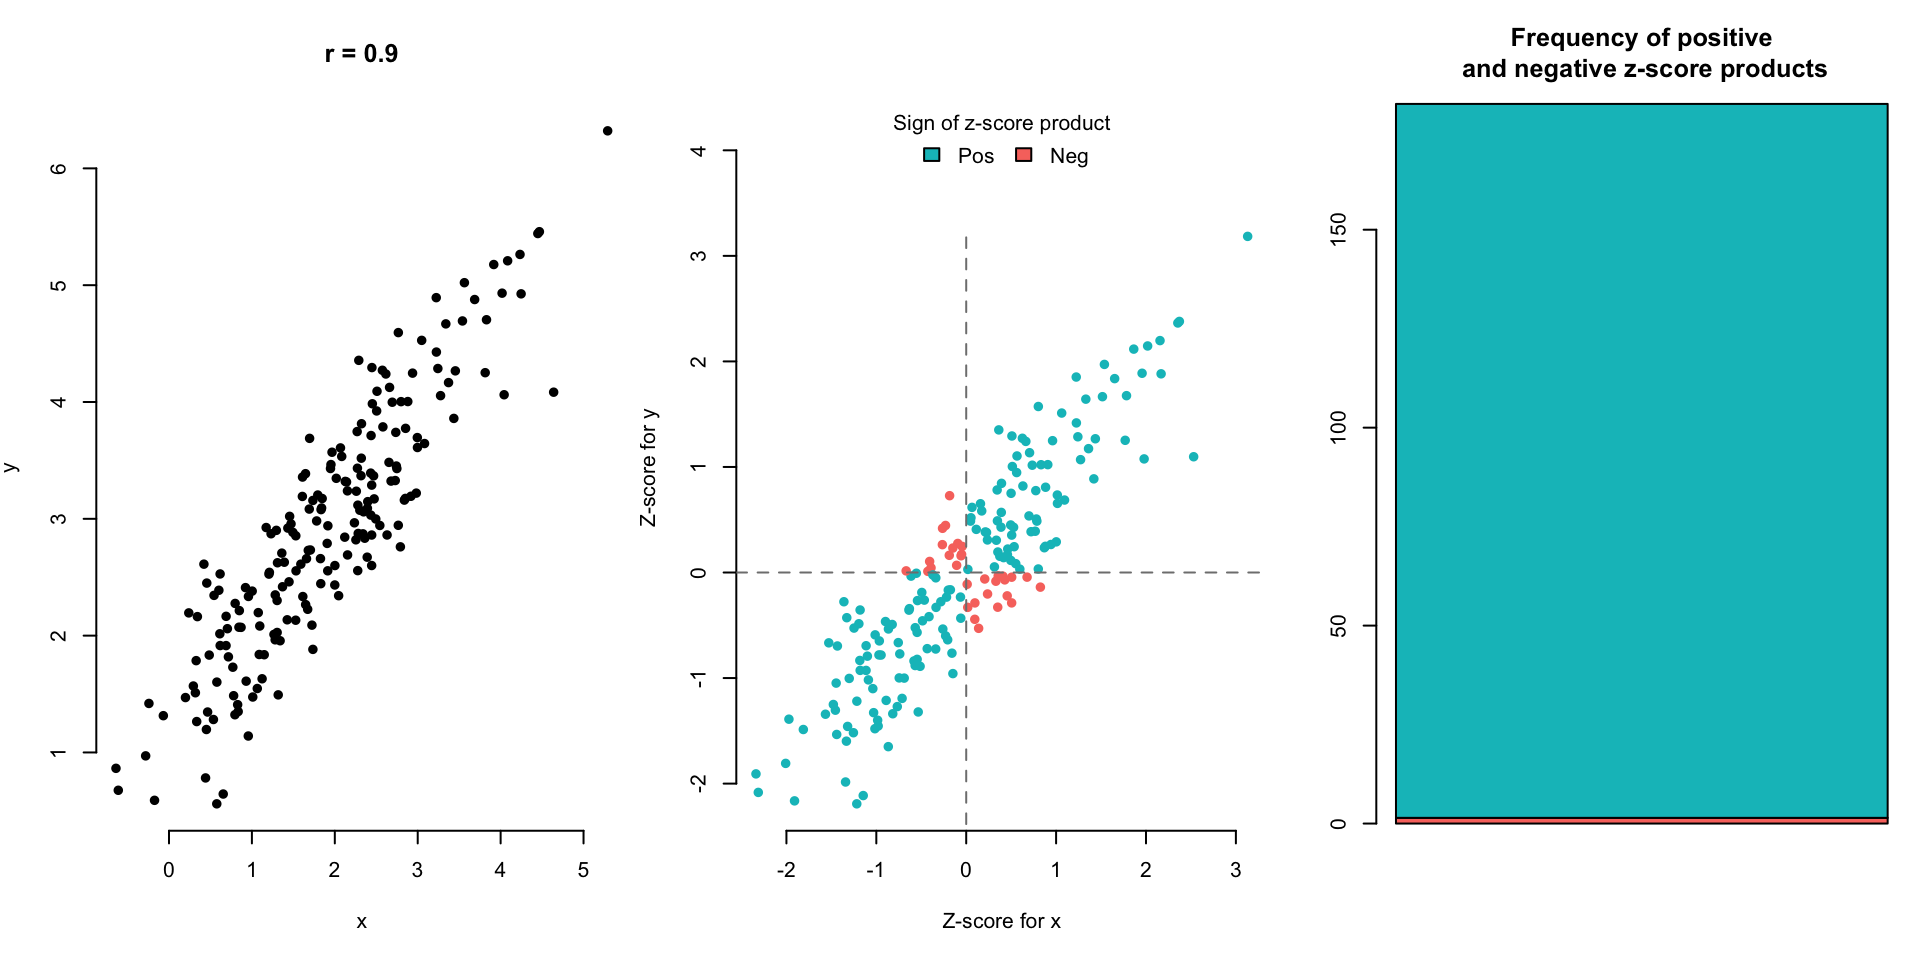
\includegraphics{02-visualization_files/figure-latex/unnamed-chunk-65-3.pdf} 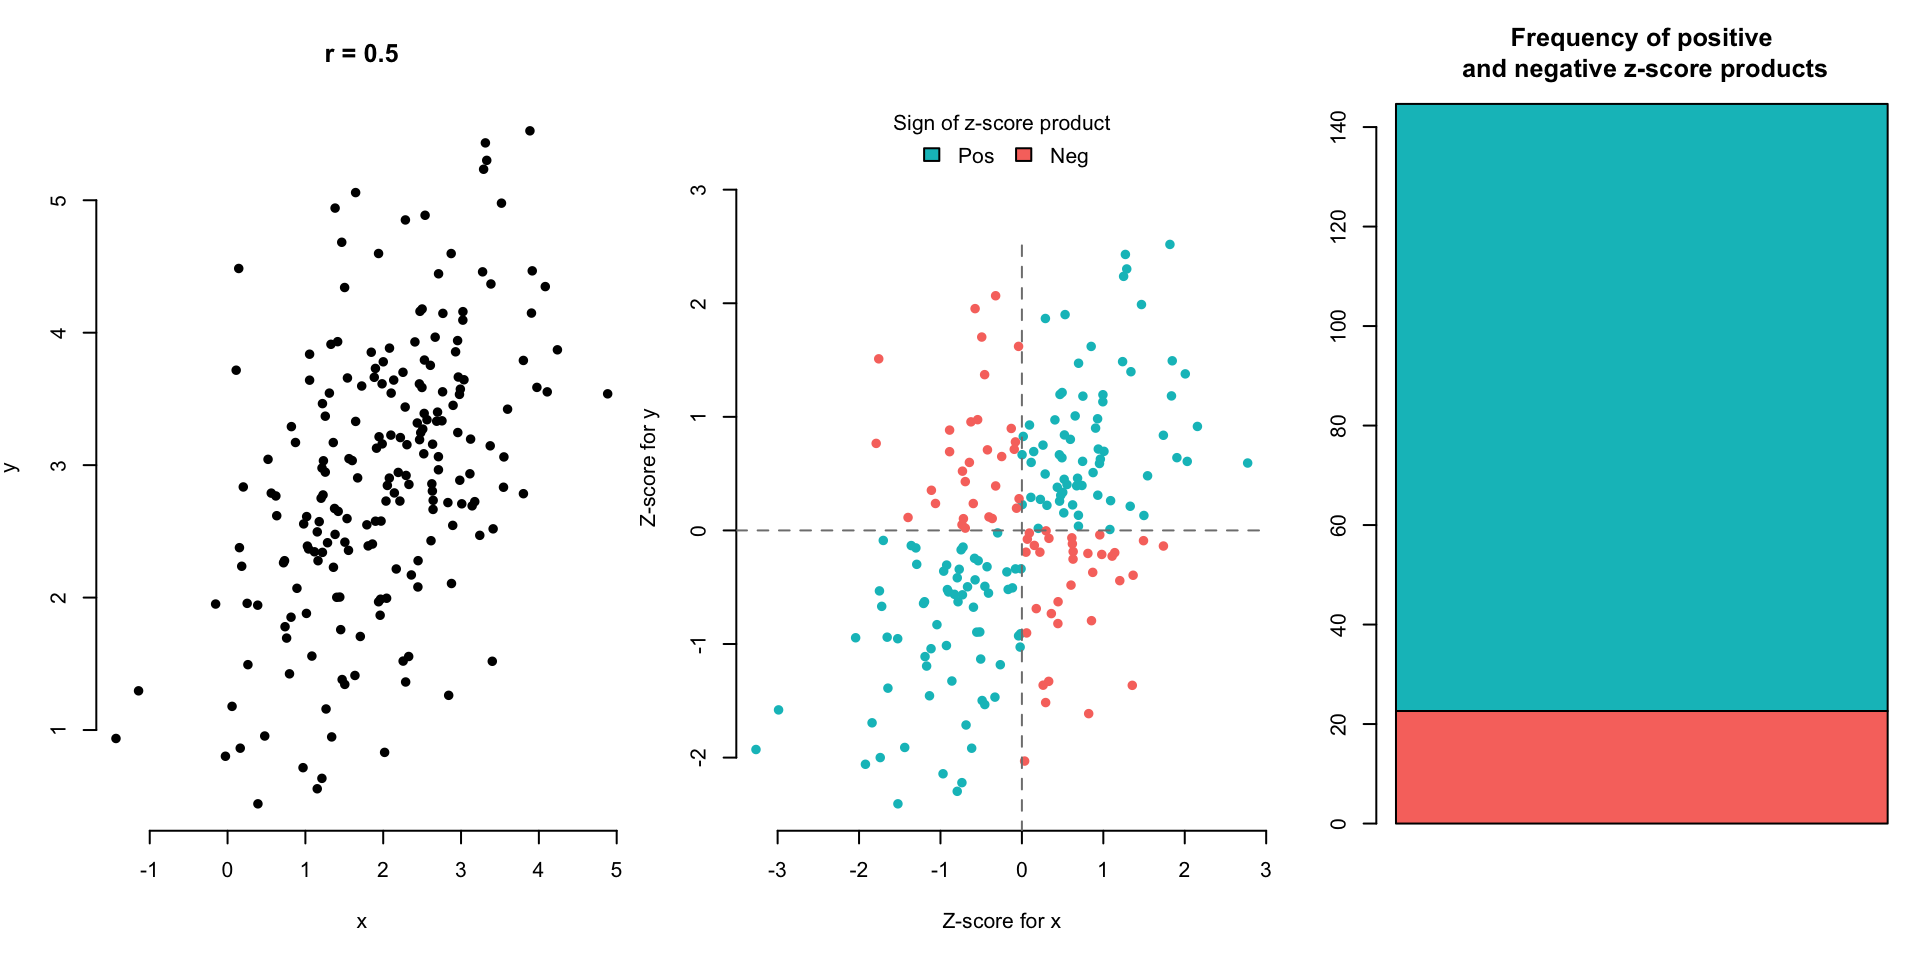
\includegraphics{02-visualization_files/figure-latex/unnamed-chunk-65-4.pdf} 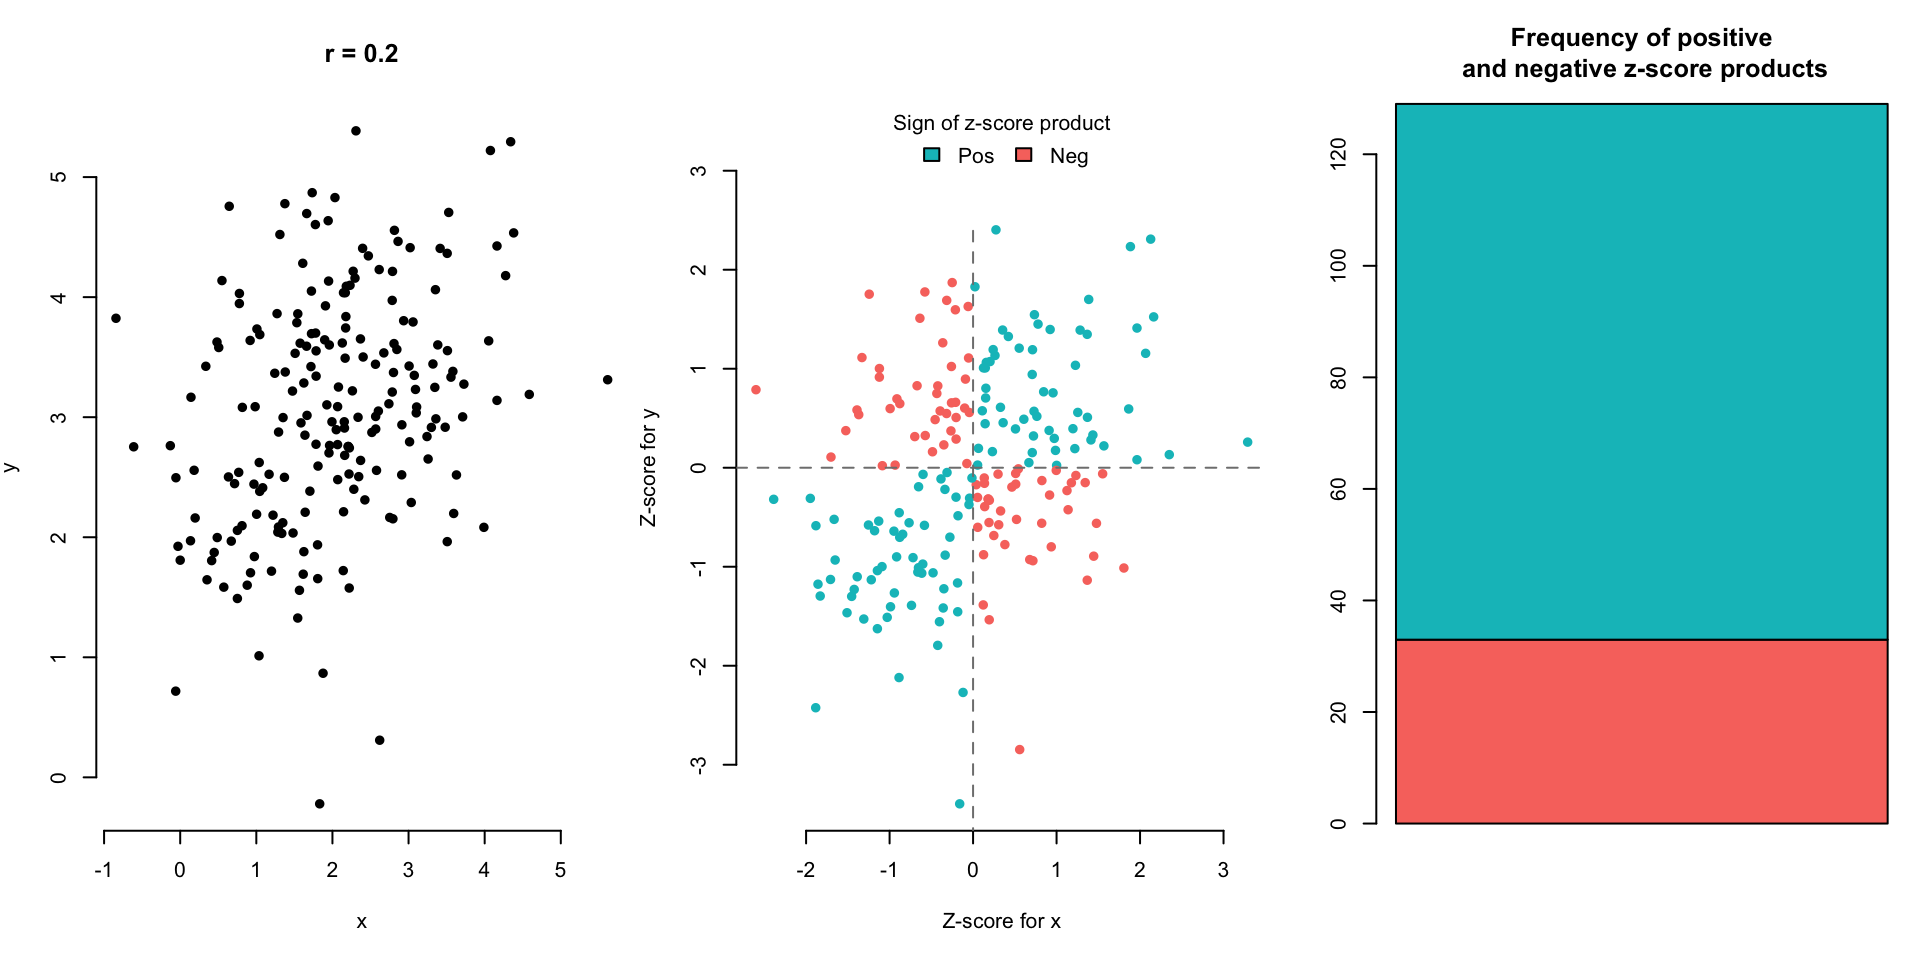
\includegraphics{02-visualization_files/figure-latex/unnamed-chunk-65-5.pdf} 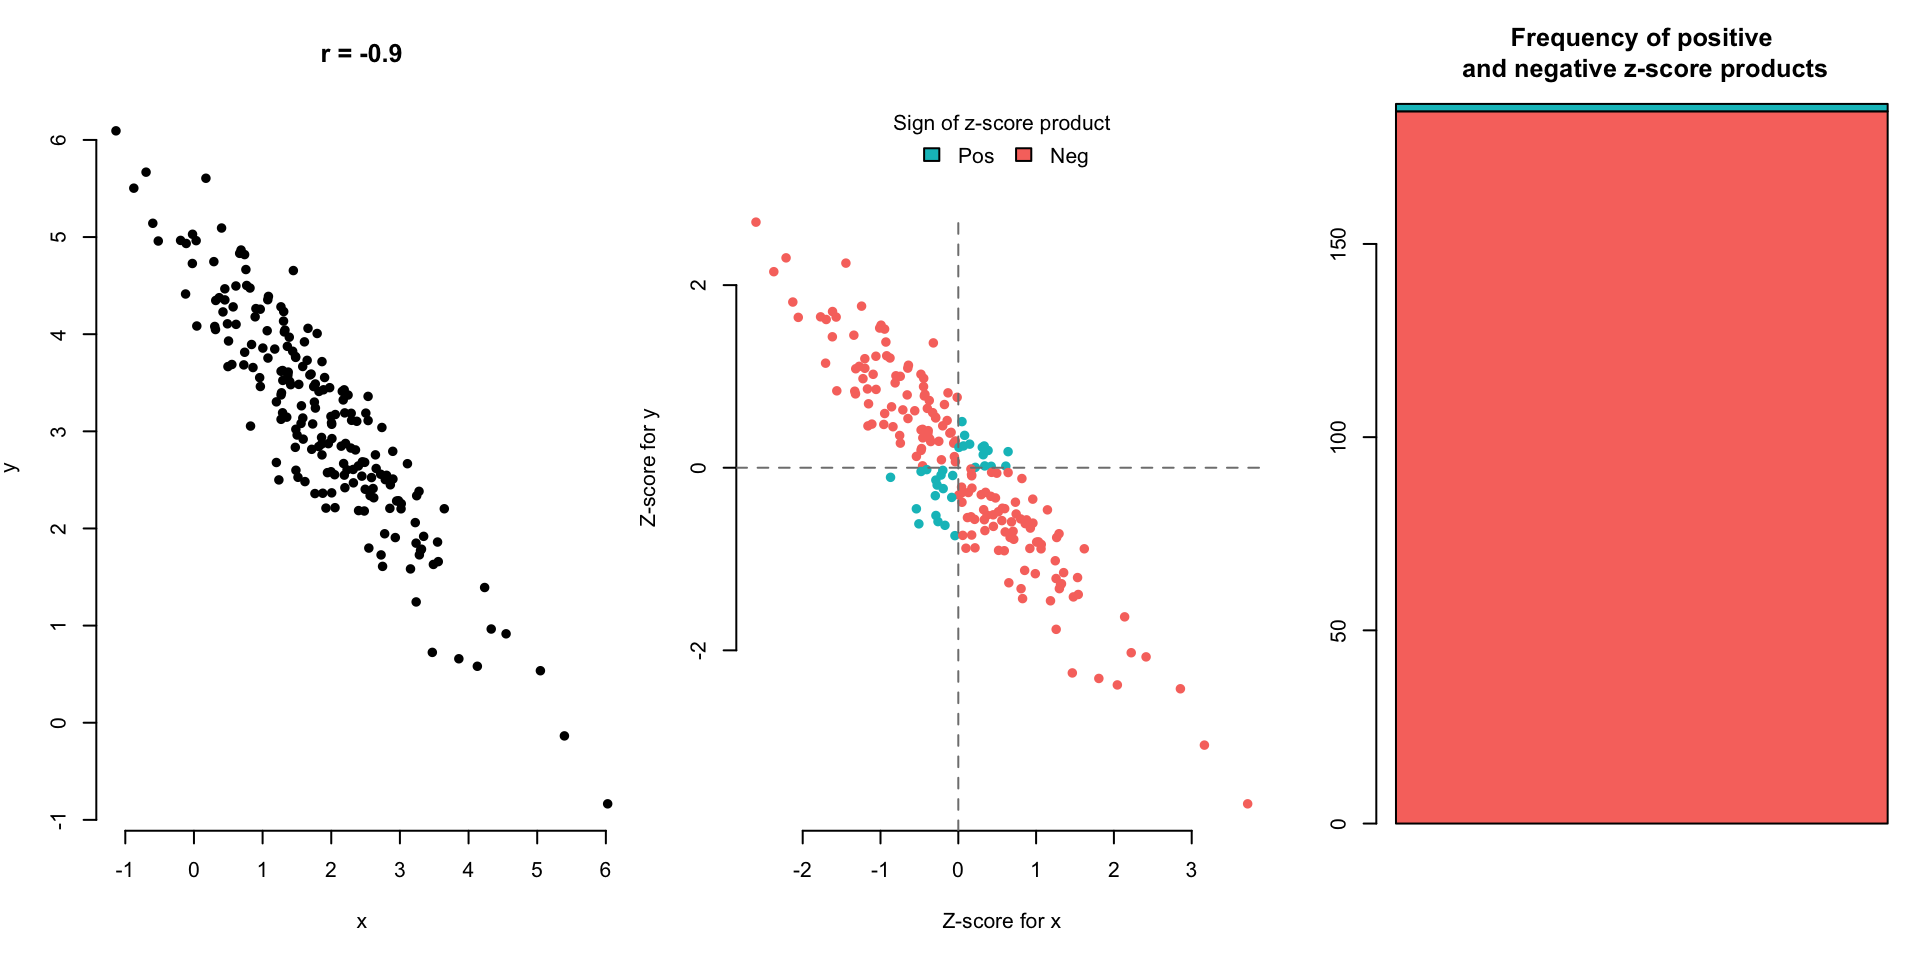
\includegraphics{02-visualization_files/figure-latex/unnamed-chunk-65-6.pdf} 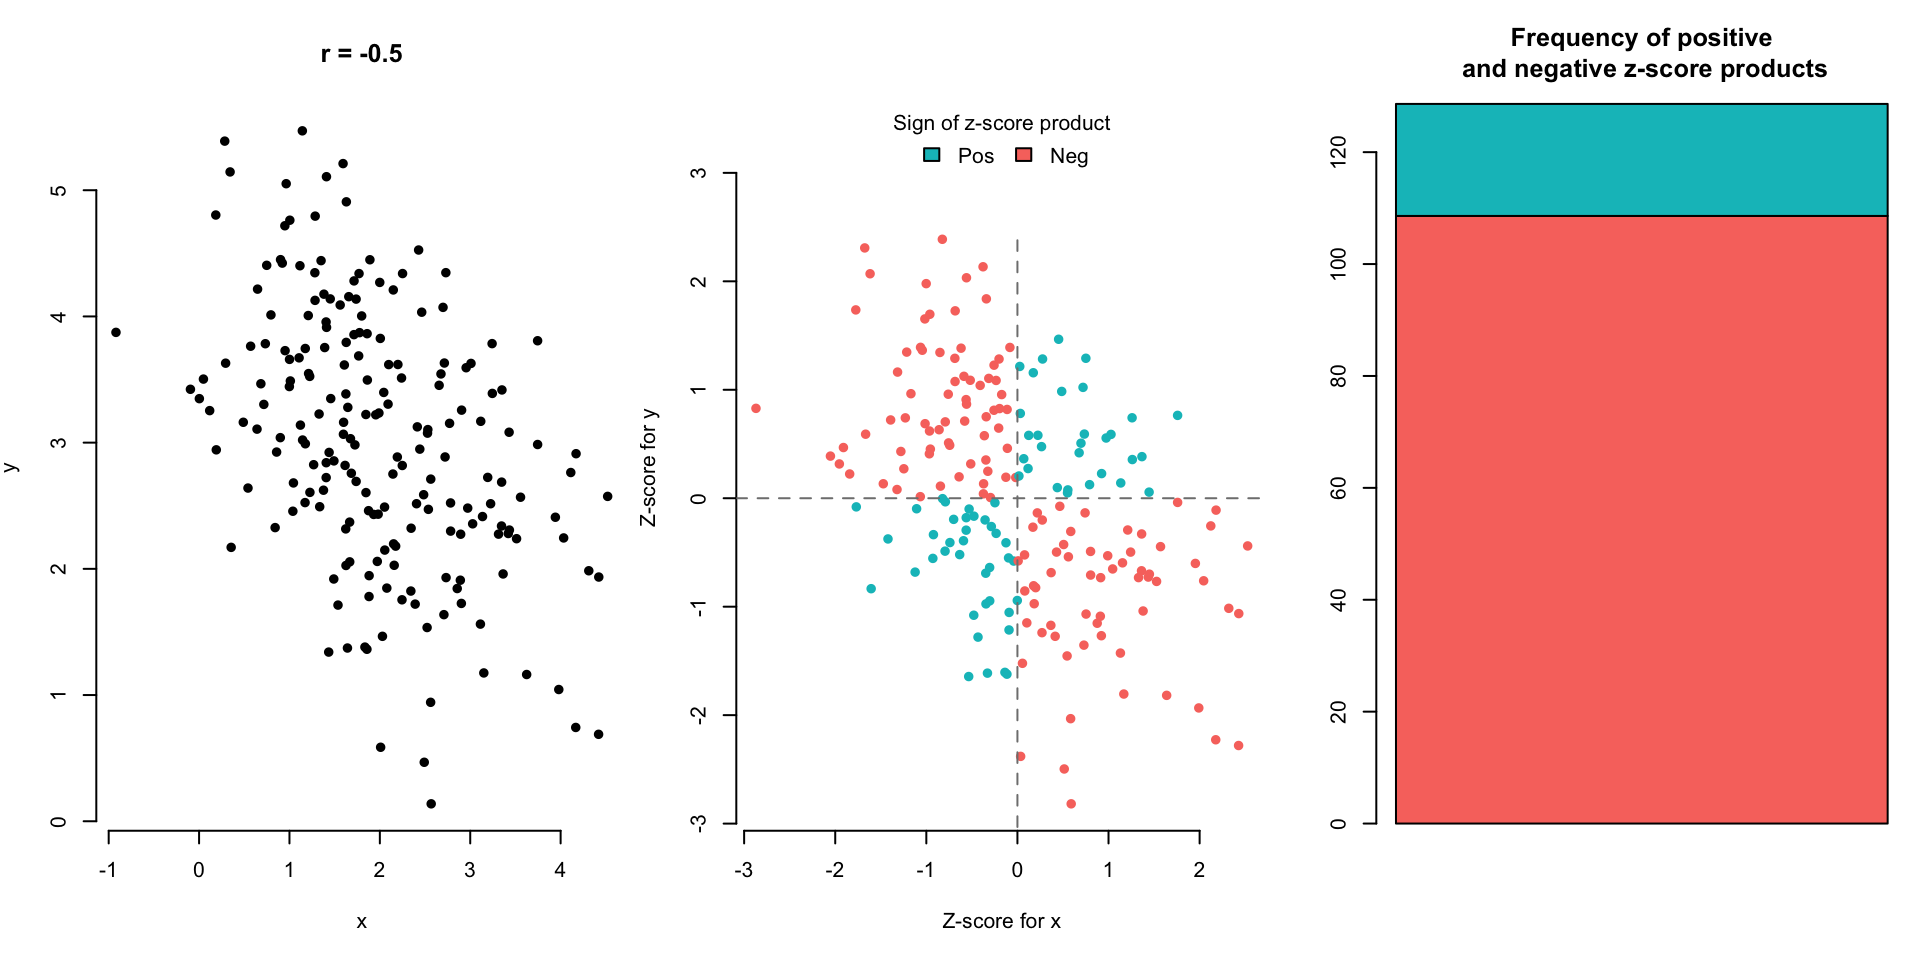
\includegraphics{02-visualization_files/figure-latex/unnamed-chunk-65-7.pdf} 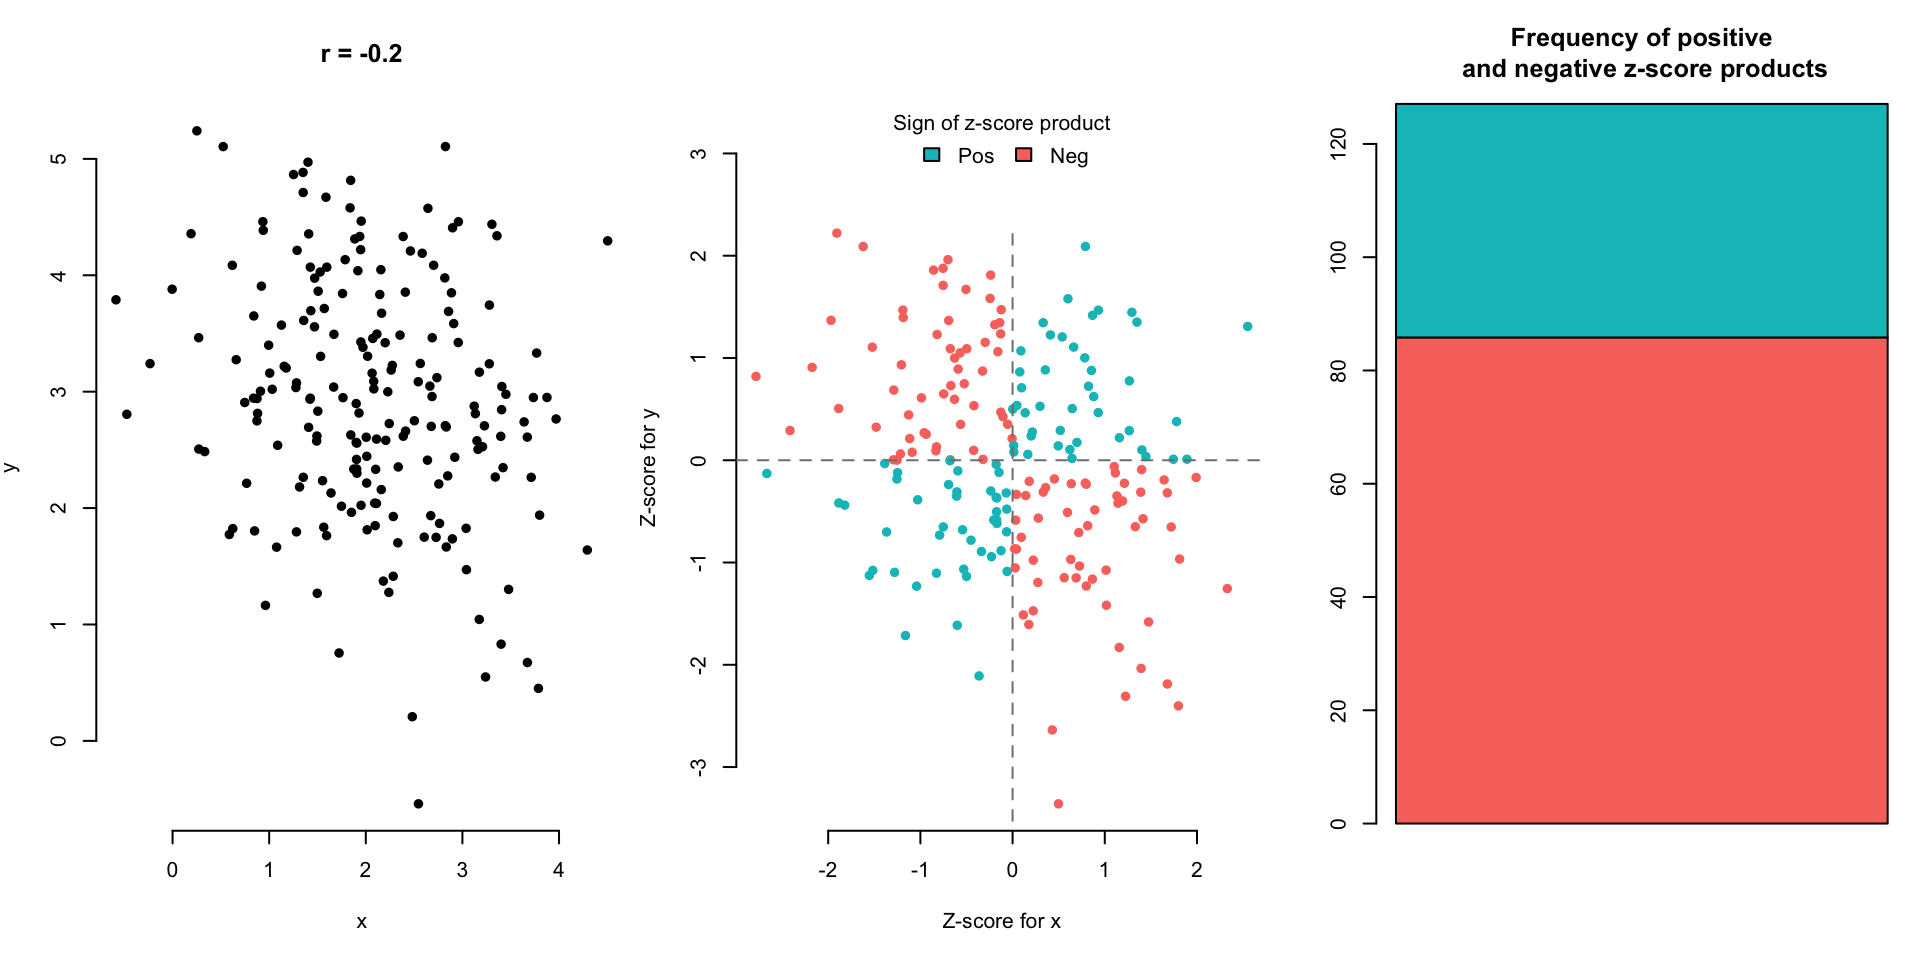
\includegraphics{02-visualization_files/figure-latex/unnamed-chunk-65-8.pdf}

\begin{mathbox}
(Optional) Here are other equivalent expressions for \(r\) for the
mathematically intrigued:

\[ r = \frac{\sum z_x z_y}{n-1}  \]
\[ = \frac{\sum{\frac{(x_i-\bar{x})}{s_x}\times\frac{(y_i-\bar{y})}{s_y}}}{n-1}\]
\[= \frac{\sum{(x_i-\bar{x})(y_i-\bar{y})}}{(n-1) s_x s_y}\]
\[= \frac{\sum{(x_i-\bar{x})(y_i-\bar{y})}}{(n-1)\sqrt{\sum{\frac{(x_i-\bar{x})^2}{n-1}}}\sqrt{\sum{\frac{(y_i-\bar{y})^2}{n-1}}}}\]
\[=\frac{\sum{(x_i-\bar{x})(y_i-\bar{y})}}{\sqrt{\sum{(x_i-\bar{x})^2}}\sqrt{\sum{(y_i-\bar{y})^2}}}\]
\[=\frac{\sum{(x_i-\bar{x})(y_i-\bar{y})}}{\sqrt{\sum{(x_i-\bar{x})^2\sum{(y_i-\bar{y})^2}}}}\]
\end{mathbox}

\hypertarget{is-correlation-always-the-right-way-to-judge-strength}{%
\subsection{Is correlation always the right way to judge strength?}\label{is-correlation-always-the-right-way-to-judge-strength}}

The plot below shows the relationship between brownie quality and oven temperature at which the brownie is baked.

The correlation coefficient is near 0, but it doesn't mean that there's no relationship. We can clearly see a quadratic relationship, but there's not a \textbf{linear} relationship.

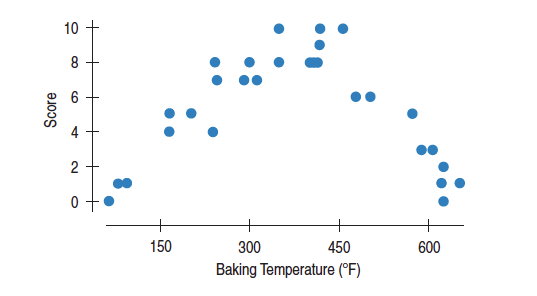
\includegraphics{Photos/Brownies.png}

The correlation coefficient, \(r\), is more formally called the Pearson correlation coefficient, named after Karl Pearson who published this work in 1895. Read more about this measure of linear relationship \href{https://en.wikipedia.org/wiki/Pearson_correlation_coefficient}{here}.

\hypertarget{three-or-more-variables}{%
\section{Three or more variables}\label{three-or-more-variables}}

In complex data sets that contain many variables, it is necessary to get a fuller understanding of the relationships in the data than we can see with plots that look at only one or two variables.

The following visual features can help us turn bivariate plots into multivariate plots:

\begin{itemize}
\tightlist
\item
  Color of points and lines
\item
  Shape of points
\item
  Size of points
\item
  Panels (facets)
\end{itemize}

Let's look at another data set, the 1985 Current Population Survey. This is a smaller scale survey administered by the United States government in the intervening years of the decennial census.

\hypertarget{a-bivariate-scatterplot}{%
\subsection{A bivariate scatterplot}\label{a-bivariate-scatterplot}}

Our primary interest is the \texttt{wage} variable which gives the hourly wage for each individual in the data set in US dollars. What is the relationship between years of education and hourly wage?

\begin{Shaded}
\begin{Highlighting}[]
\KeywordTok{data}\NormalTok{(CPS85) }\CommentTok{# Load the data from the R package CPS85}

\NormalTok{CPS85 }\OperatorTok
\StringTok{    }\KeywordTok{ggplot}\NormalTok{(}\KeywordTok{aes}\NormalTok{(}\DataTypeTok{x =}\NormalTok{ educ, }\DataTypeTok{y =}\NormalTok{ wage)) }\OperatorTok{+}
\StringTok{    }\KeywordTok{geom_point}\NormalTok{() }\OperatorTok{+}
\StringTok{    }\KeywordTok{xlab}\NormalTok{(}\StringTok{"Years of education"}\NormalTok{) }\OperatorTok{+}
\StringTok{    }\KeywordTok{ylab}\NormalTok{(}\StringTok{"Hourly wage (US dollars)"}\NormalTok{) }\OperatorTok{+}
\StringTok{    }\KeywordTok{theme_minimal}\NormalTok{()}
\end{Highlighting}
\end{Shaded}

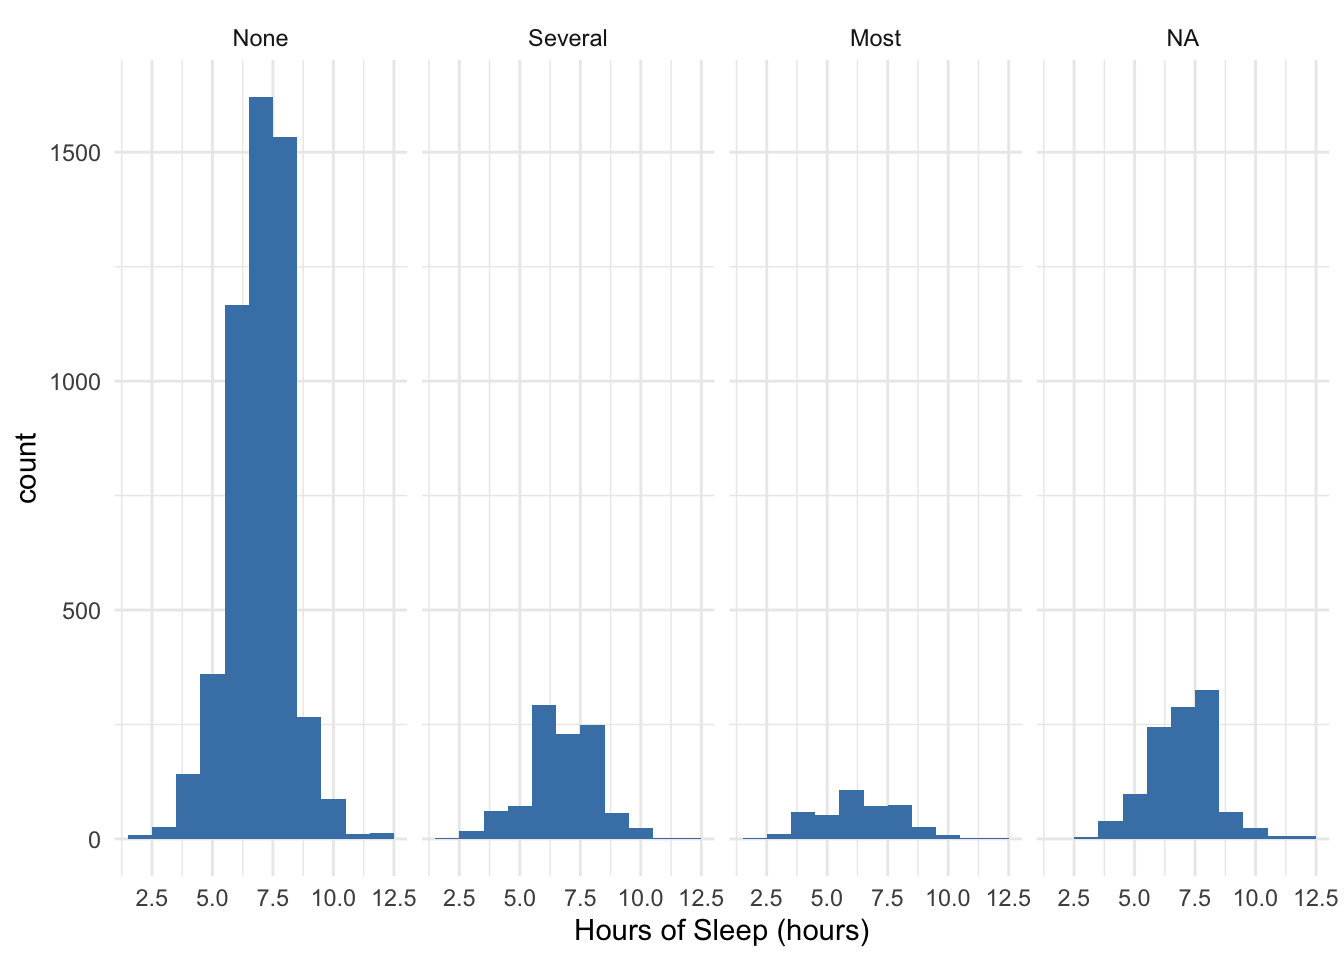
\includegraphics{02-visualization_files/figure-latex/unnamed-chunk-67-1.pdf}

We can see that years of education and hourly wage are positively correlated. What about the impact of other variables?

\hypertarget{enriching-with-color}{%
\subsection{Enriching with color}\label{enriching-with-color}}

We can enrich this bivariate scatterplot by showing additional information via color.

\begin{Shaded}
\begin{Highlighting}[]
\NormalTok{CPS85 }\OperatorTok
\StringTok{    }\KeywordTok{ggplot}\NormalTok{(}\KeywordTok{aes}\NormalTok{(}\DataTypeTok{x =}\NormalTok{ educ, }\DataTypeTok{y =}\NormalTok{ wage, }\DataTypeTok{color =}\NormalTok{ age)) }\OperatorTok{+}
\StringTok{    }\KeywordTok{geom_point}\NormalTok{() }\OperatorTok{+}
\StringTok{    }\KeywordTok{xlab}\NormalTok{(}\StringTok{"Years of education"}\NormalTok{) }\OperatorTok{+}
\StringTok{    }\KeywordTok{ylab}\NormalTok{(}\StringTok{"Hourly wage (US dollars)"}\NormalTok{) }\OperatorTok{+}
\StringTok{    }\KeywordTok{theme_minimal}\NormalTok{()}
\end{Highlighting}
\end{Shaded}

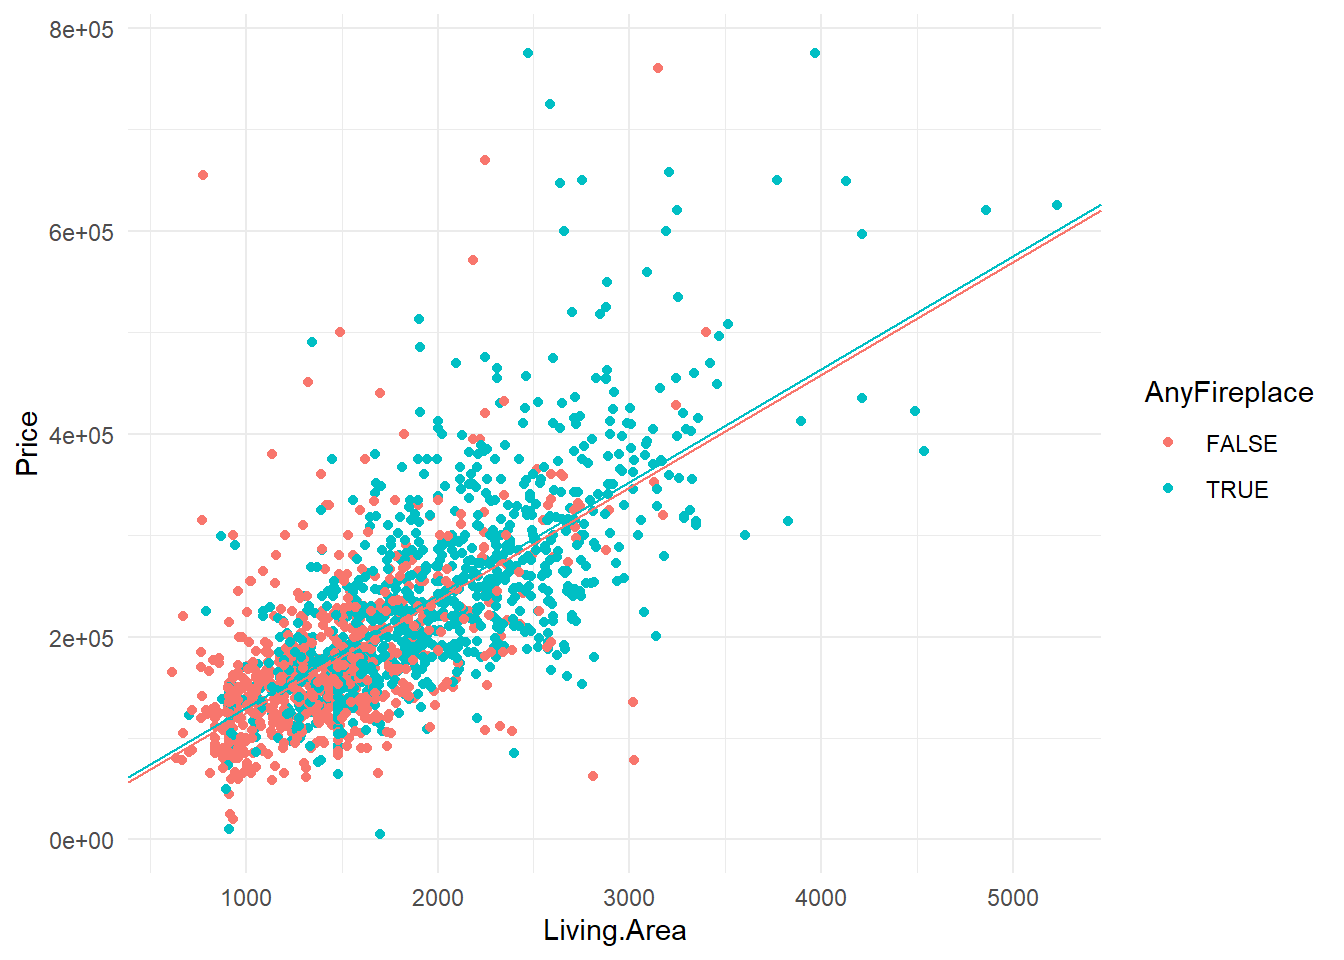
\includegraphics{02-visualization_files/figure-latex/unnamed-chunk-68-1.pdf}

Adding color for a quantitative variable, age, does not reveal any obvious patterns; that is, we don't see obvious clustering by color. Perhaps this is because there are too many colors (remember Visualization Principle \#6: Use Color Appropriately). Are any patterns revealed if we use 4 age categories instead?

\begin{Shaded}
\begin{Highlighting}[]
\NormalTok{CPS85 }\OperatorTok
\StringTok{    }\KeywordTok{mutate}\NormalTok{(}\DataTypeTok{age_cat =} \KeywordTok{cut}\NormalTok{(age, }\DecValTok{4}\NormalTok{)) }\OperatorTok
\StringTok{    }\KeywordTok{ggplot}\NormalTok{(}\KeywordTok{aes}\NormalTok{(}\DataTypeTok{x =}\NormalTok{ educ, }\DataTypeTok{y =}\NormalTok{ wage, }\DataTypeTok{color =}\NormalTok{ age_cat)) }\OperatorTok{+}
\StringTok{    }\KeywordTok{geom_point}\NormalTok{() }\OperatorTok{+}
\StringTok{    }\KeywordTok{xlab}\NormalTok{(}\StringTok{"Years of education"}\NormalTok{) }\OperatorTok{+}
\StringTok{    }\KeywordTok{ylab}\NormalTok{(}\StringTok{"Hourly wage (US dollars)"}\NormalTok{) }\OperatorTok{+}
\StringTok{    }\KeywordTok{guides}\NormalTok{(}\DataTypeTok{color =} \KeywordTok{guide_legend}\NormalTok{(}\DataTypeTok{title =} \StringTok{"Age category"}\NormalTok{)) }\OperatorTok{+}\StringTok{ }\CommentTok{# Legend title}
\StringTok{    }\KeywordTok{theme_minimal}\NormalTok{()}
\end{Highlighting}
\end{Shaded}

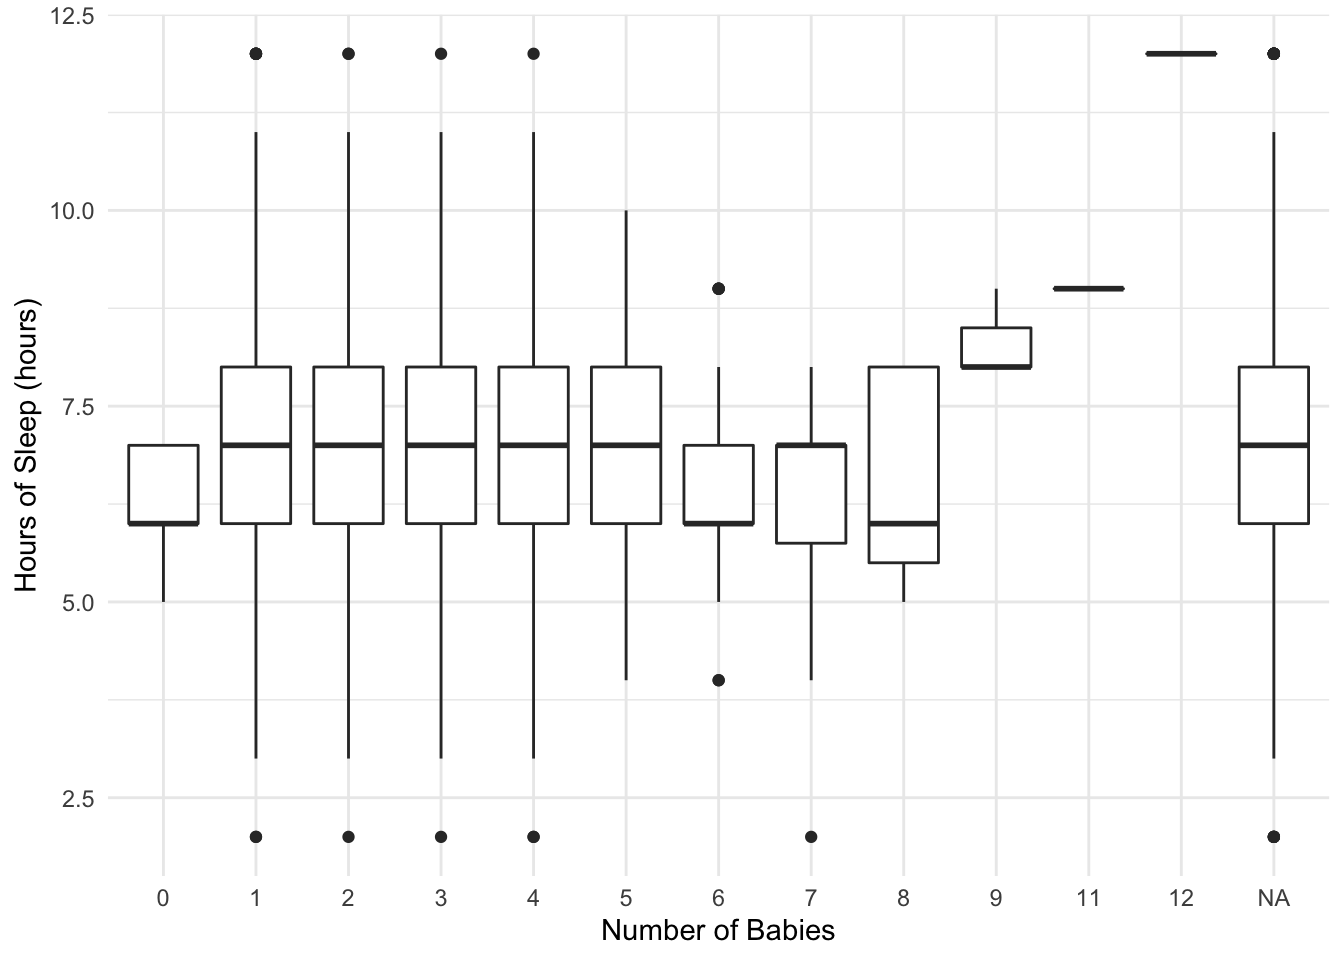
\includegraphics{02-visualization_files/figure-latex/unnamed-chunk-69-1.pdf}

With 4 age categories, no age patterns are evident, but this does help us see that the least educated people in this data set are mostly in the youngest and oldest age categories.

\hypertarget{enriching-with-shape}{%
\subsection{Enriching with shape}\label{enriching-with-shape}}

We can also encode information via point shape. Here we let shape encode marital status.

\begin{Shaded}
\begin{Highlighting}[]
\NormalTok{CPS85 }\OperatorTok
\StringTok{    }\KeywordTok{ggplot}\NormalTok{(}\KeywordTok{aes}\NormalTok{(}\DataTypeTok{x =}\NormalTok{ educ, }\DataTypeTok{y =}\NormalTok{ wage, }\DataTypeTok{shape =}\NormalTok{ married)) }\OperatorTok{+}
\StringTok{    }\KeywordTok{geom_point}\NormalTok{() }\OperatorTok{+}
\StringTok{    }\KeywordTok{xlab}\NormalTok{(}\StringTok{"Years of education"}\NormalTok{) }\OperatorTok{+}
\StringTok{    }\KeywordTok{ylab}\NormalTok{(}\StringTok{"Hourly wage (US dollars)"}\NormalTok{) }\OperatorTok{+}
\StringTok{    }\KeywordTok{guides}\NormalTok{(}\DataTypeTok{shape =} \KeywordTok{guide_legend}\NormalTok{(}\DataTypeTok{title =} \StringTok{"Marital status"}\NormalTok{)) }\OperatorTok{+}\StringTok{ }\CommentTok{# Legend title}
\StringTok{    }\KeywordTok{theme_minimal}\NormalTok{()}
\end{Highlighting}
\end{Shaded}

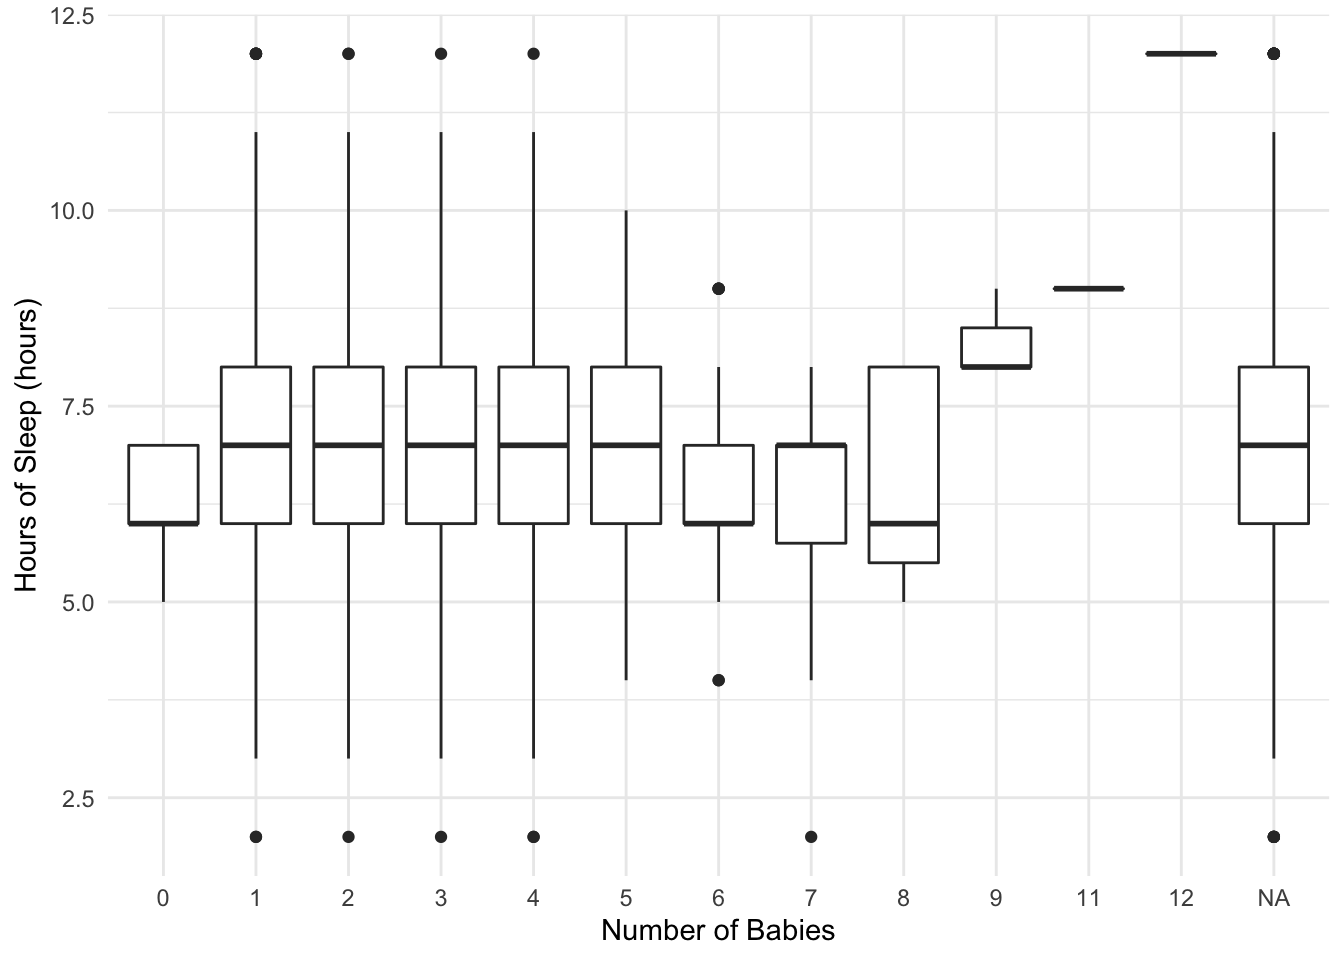
\includegraphics{02-visualization_files/figure-latex/unnamed-chunk-70-1.pdf}

Often encoding information with color is preferable to encoding it with shapes because differences in shapes are not as easily discernible. Remember that statistical visualizations are meant to help you better understand your data. If you are having trouble easily picking out patterns when using a certain visual feature (e.g.~shape, color), try another feature to see if the clarity of the plot increases for you.

\hypertarget{enriching-with-size}{%
\subsection{Enriching with size}\label{enriching-with-size}}

The size of a point is useful for conveying the magnitude of a quantitative variable. For example, we may wish to see non-categorized age information with point size.

\begin{Shaded}
\begin{Highlighting}[]
\NormalTok{CPS85 }\OperatorTok
\StringTok{    }\KeywordTok{ggplot}\NormalTok{(}\KeywordTok{aes}\NormalTok{(}\DataTypeTok{x =}\NormalTok{ educ, }\DataTypeTok{y =}\NormalTok{ wage, }\DataTypeTok{size =}\NormalTok{ age)) }\OperatorTok{+}
\StringTok{    }\KeywordTok{geom_point}\NormalTok{(}\DataTypeTok{alpha =} \FloatTok{0.5}\NormalTok{) }\OperatorTok{+}\StringTok{ }\CommentTok{#alpha specifies the level of transparency of the points}
\StringTok{    }\KeywordTok{xlab}\NormalTok{(}\StringTok{"Years of education"}\NormalTok{) }\OperatorTok{+}
\StringTok{    }\KeywordTok{ylab}\NormalTok{(}\StringTok{"Hourly wage (US dollars)"}\NormalTok{) }\OperatorTok{+}
\StringTok{    }\KeywordTok{guides}\NormalTok{(}\DataTypeTok{size =} \KeywordTok{guide_legend}\NormalTok{(}\DataTypeTok{title =} \StringTok{"Age"}\NormalTok{)) }\OperatorTok{+}\StringTok{ }\CommentTok{# Legend title}
\StringTok{    }\KeywordTok{theme_minimal}\NormalTok{()}
\end{Highlighting}
\end{Shaded}

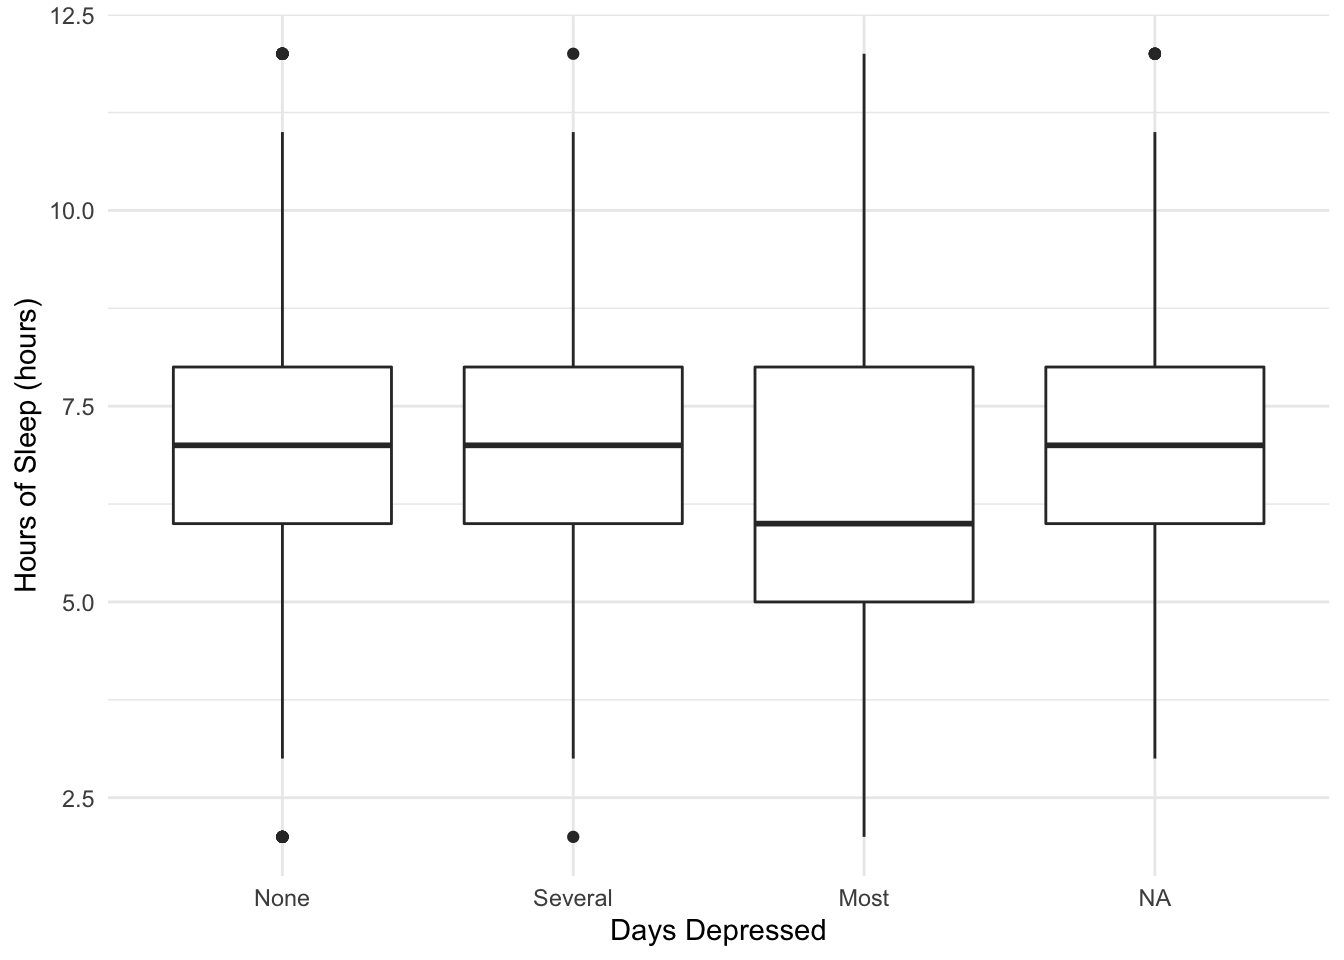
\includegraphics{02-visualization_files/figure-latex/unnamed-chunk-71-1.pdf}

\hypertarget{enriching-with-panels}{%
\subsection{Enriching with panels}\label{enriching-with-panels}}

Panels (or facets) are a great way to see how relationships differ between levels of a single categorical variable or between combinations of two categorical variables.

Let's look at the relationship between hourly wage and years of education across job sectors. The following creates a row of plots of this relationship over job sectors.

\begin{Shaded}
\begin{Highlighting}[]
\NormalTok{CPS85 }\OperatorTok
\StringTok{    }\KeywordTok{ggplot}\NormalTok{(}\KeywordTok{aes}\NormalTok{(}\DataTypeTok{x =}\NormalTok{ educ, }\DataTypeTok{y =}\NormalTok{ wage)) }\OperatorTok{+}
\StringTok{    }\KeywordTok{geom_point}\NormalTok{() }\OperatorTok{+}
\StringTok{    }\KeywordTok{xlab}\NormalTok{(}\StringTok{"Years of education"}\NormalTok{) }\OperatorTok{+}
\StringTok{    }\KeywordTok{ylab}\NormalTok{(}\StringTok{"Hourly wage (US dollars)"}\NormalTok{) }\OperatorTok{+}
\StringTok{    }\KeywordTok{facet_grid}\NormalTok{(. }\OperatorTok{~}\StringTok{ }\NormalTok{sector) }\OperatorTok{+}
\StringTok{    }\KeywordTok{theme_minimal}\NormalTok{()}
\end{Highlighting}
\end{Shaded}

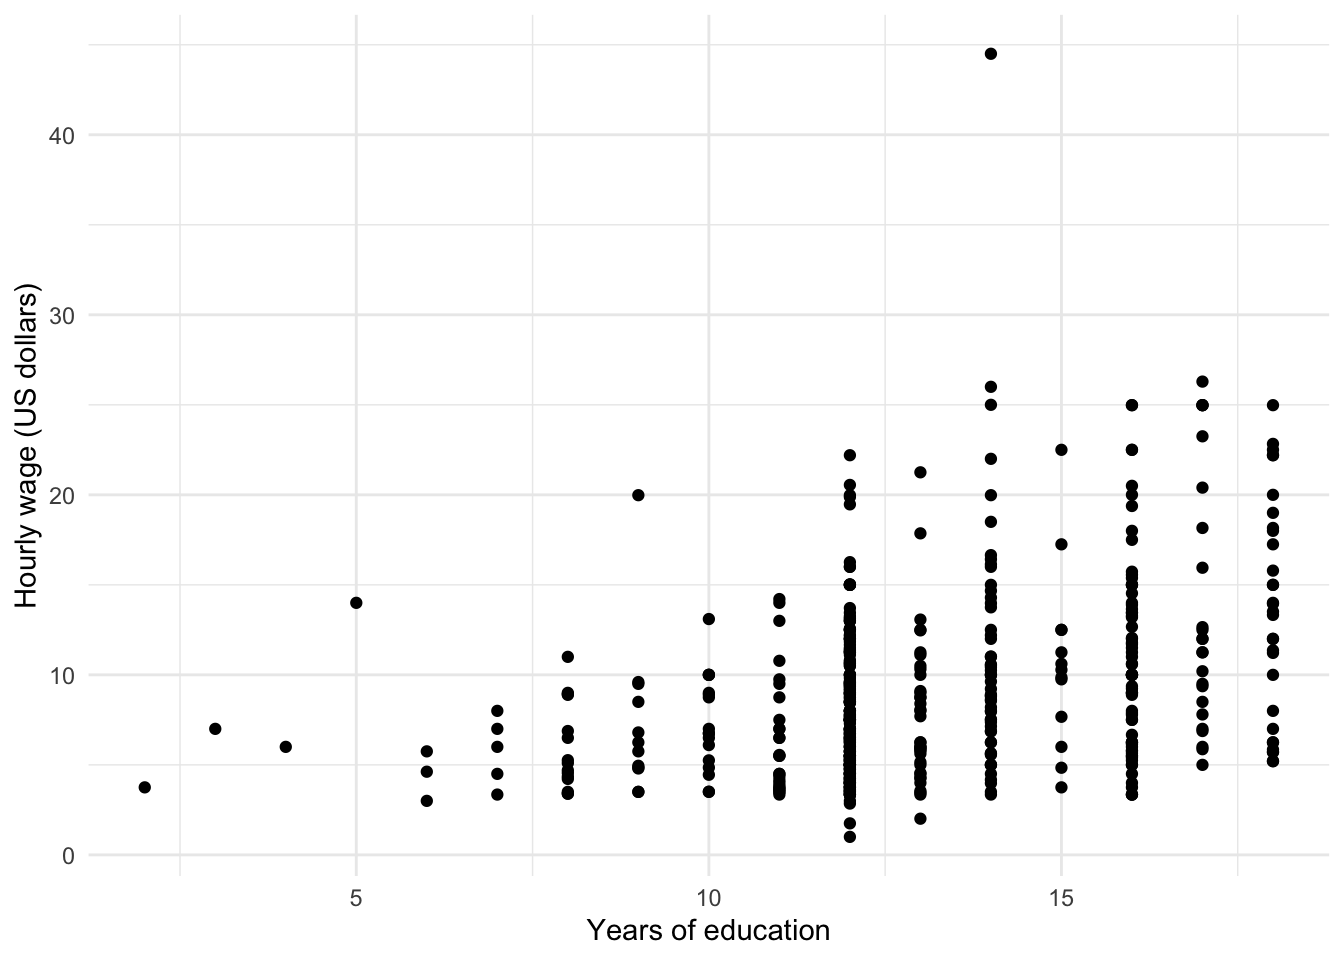
\includegraphics{02-visualization_files/figure-latex/unnamed-chunk-72-1.pdf}

With a small change in notation (\texttt{sector\ \textasciitilde{}\ .} versus \texttt{.\ \textasciitilde{}\ sector}), we can create a column of plots.

\begin{Shaded}
\begin{Highlighting}[]
\NormalTok{CPS85 }\OperatorTok
\StringTok{    }\KeywordTok{ggplot}\NormalTok{(}\KeywordTok{aes}\NormalTok{(}\DataTypeTok{x =}\NormalTok{ educ, }\DataTypeTok{y =}\NormalTok{ wage)) }\OperatorTok{+}
\StringTok{    }\KeywordTok{geom_point}\NormalTok{() }\OperatorTok{+}
\StringTok{    }\KeywordTok{xlab}\NormalTok{(}\StringTok{"Years of education"}\NormalTok{) }\OperatorTok{+}
\StringTok{    }\KeywordTok{ylab}\NormalTok{(}\StringTok{"Hourly wage (US dollars)"}\NormalTok{) }\OperatorTok{+}
\StringTok{    }\KeywordTok{facet_grid}\NormalTok{(sector }\OperatorTok{~}\StringTok{ }\NormalTok{.) }\OperatorTok{+}
\StringTok{    }\KeywordTok{theme_minimal}\NormalTok{()}
\end{Highlighting}
\end{Shaded}

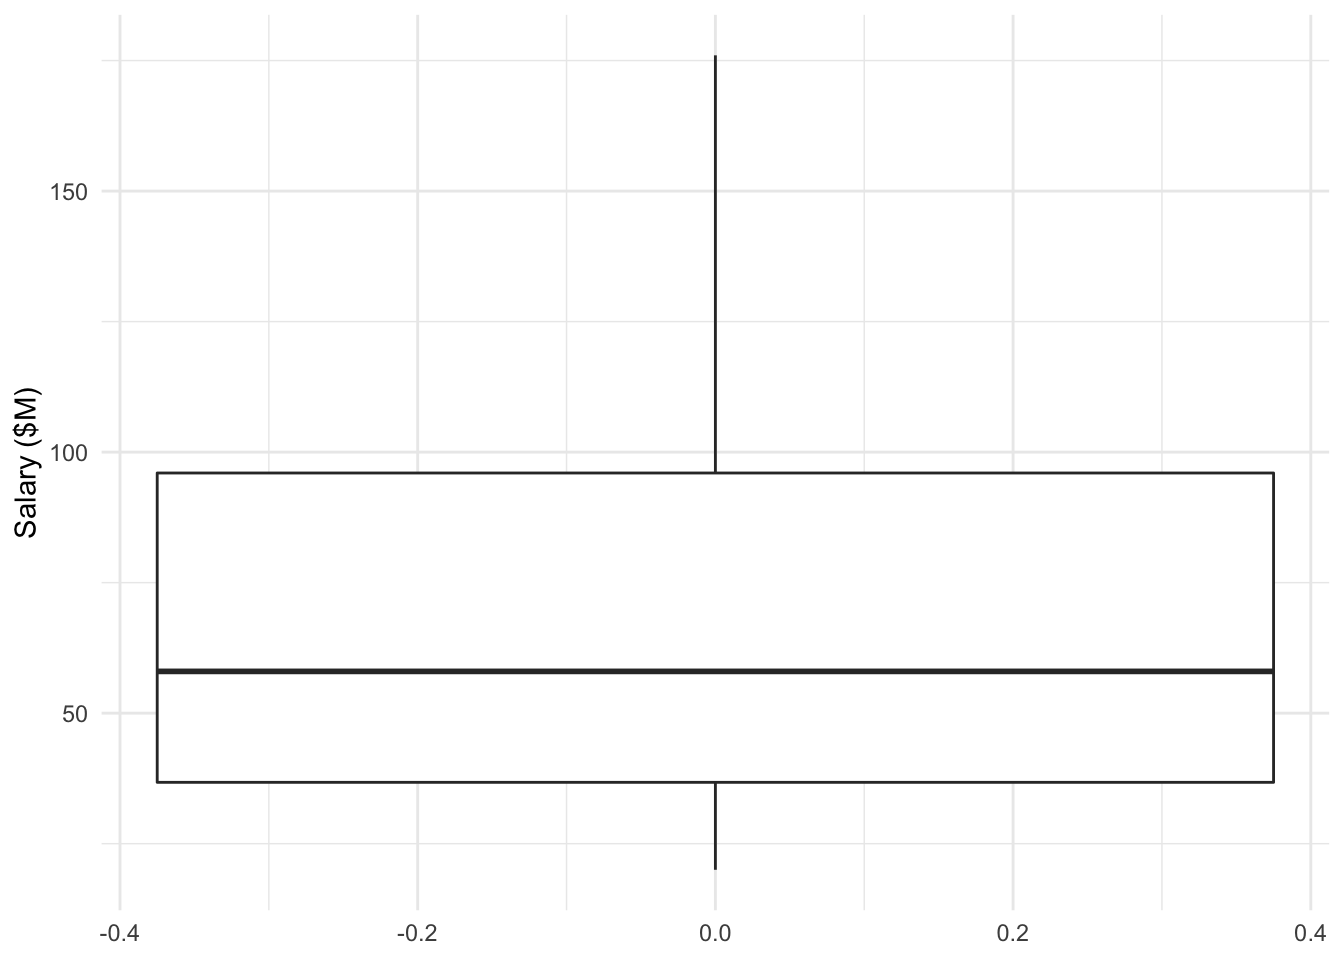
\includegraphics{02-visualization_files/figure-latex/unnamed-chunk-73-1.pdf}

We can also create panels according to two categorical variables. How do the relationships additionally differ by union status?

\begin{Shaded}
\begin{Highlighting}[]
\NormalTok{CPS85 }\OperatorTok
\StringTok{    }\KeywordTok{ggplot}\NormalTok{(}\KeywordTok{aes}\NormalTok{(}\DataTypeTok{x =}\NormalTok{ educ, }\DataTypeTok{y =}\NormalTok{ wage)) }\OperatorTok{+}
\StringTok{    }\KeywordTok{geom_point}\NormalTok{() }\OperatorTok{+}
\StringTok{    }\KeywordTok{xlab}\NormalTok{(}\StringTok{"Years of education"}\NormalTok{) }\OperatorTok{+}
\StringTok{    }\KeywordTok{ylab}\NormalTok{(}\StringTok{"Hourly wage (US dollars)"}\NormalTok{) }\OperatorTok{+}
\StringTok{    }\KeywordTok{facet_grid}\NormalTok{(sector }\OperatorTok{~}\StringTok{ }\NormalTok{union) }\OperatorTok{+}
\StringTok{    }\KeywordTok{theme_minimal}\NormalTok{()}
\end{Highlighting}
\end{Shaded}

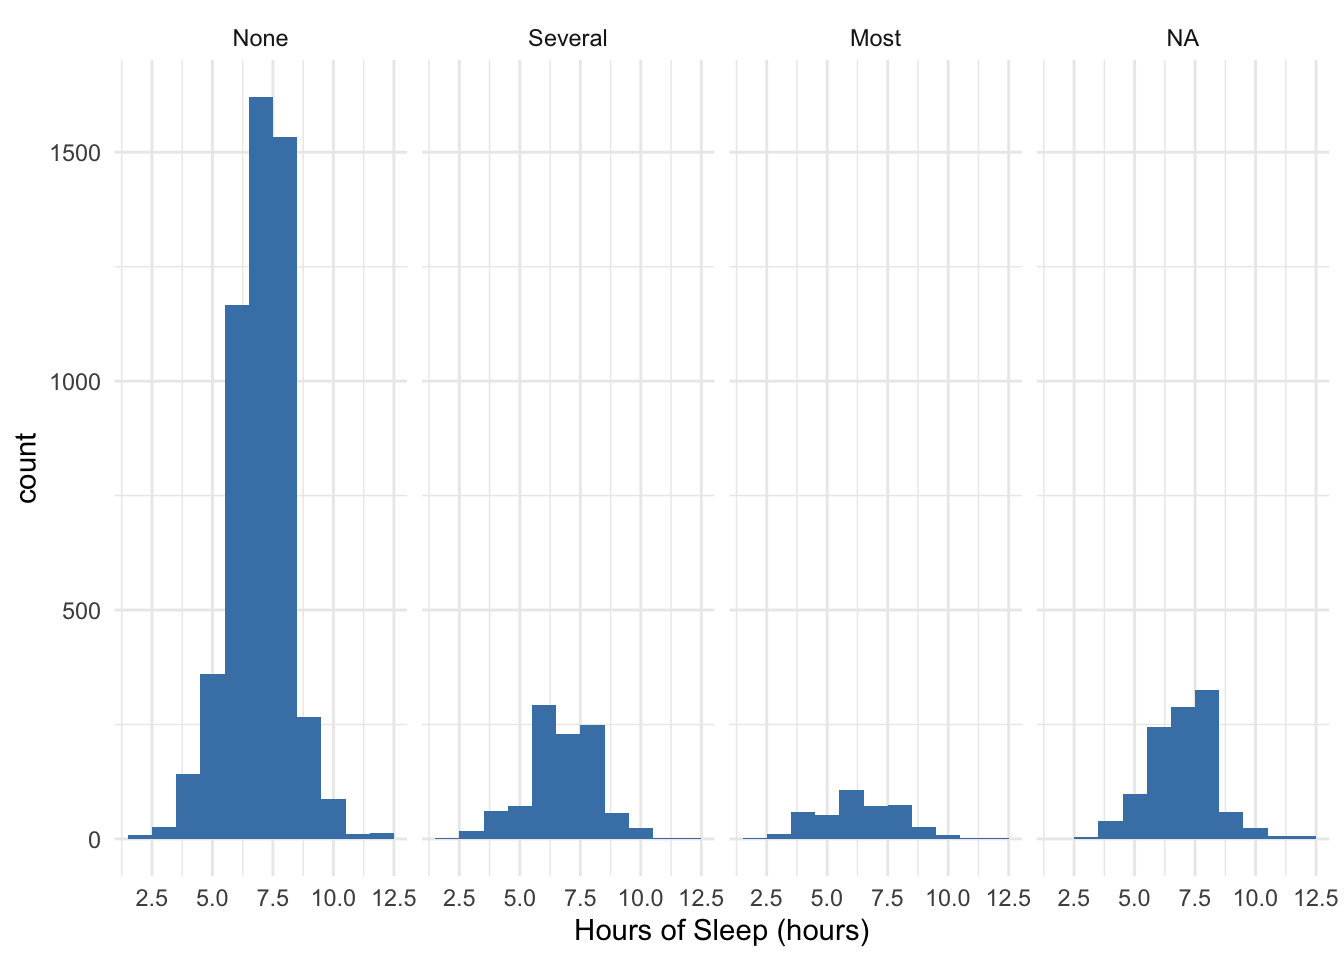
\includegraphics{02-visualization_files/figure-latex/unnamed-chunk-74-1.pdf}

\hypertarget{enriching-with-smoothing}{%
\subsection{Enriching with smoothing}\label{enriching-with-smoothing}}

If we have a scatterplot, we may want to get an understanding of the overal relationship between x and y within subsets. We can add \texttt{geom\_smooth(method\ =\ \textquotesingle{}lm\textquotesingle{})} to estimate and plot the linear relationships.

\begin{Shaded}
\begin{Highlighting}[]
\NormalTok{CPS85 }\OperatorTok
\StringTok{    }\KeywordTok{ggplot}\NormalTok{(}\KeywordTok{aes}\NormalTok{(}\DataTypeTok{x =}\NormalTok{ educ, }\DataTypeTok{y =}\NormalTok{ wage)) }\OperatorTok{+}
\StringTok{    }\KeywordTok{geom_point}\NormalTok{() }\OperatorTok{+}
\StringTok{    }\KeywordTok{geom_smooth}\NormalTok{(}\DataTypeTok{method =} \StringTok{'lm'}\NormalTok{) }\OperatorTok{+}
\StringTok{    }\KeywordTok{xlab}\NormalTok{(}\StringTok{"Years of education"}\NormalTok{) }\OperatorTok{+}
\StringTok{    }\KeywordTok{ylab}\NormalTok{(}\StringTok{"Hourly wage (US dollars)"}\NormalTok{) }\OperatorTok{+}
\StringTok{    }\KeywordTok{facet_grid}\NormalTok{(sector }\OperatorTok{~}\StringTok{ }\NormalTok{.) }\OperatorTok{+}
\StringTok{    }\KeywordTok{theme_minimal}\NormalTok{()}
\end{Highlighting}
\end{Shaded}

\begin{verbatim}
## `geom_smooth()` using formula 'y ~ x'
\end{verbatim}

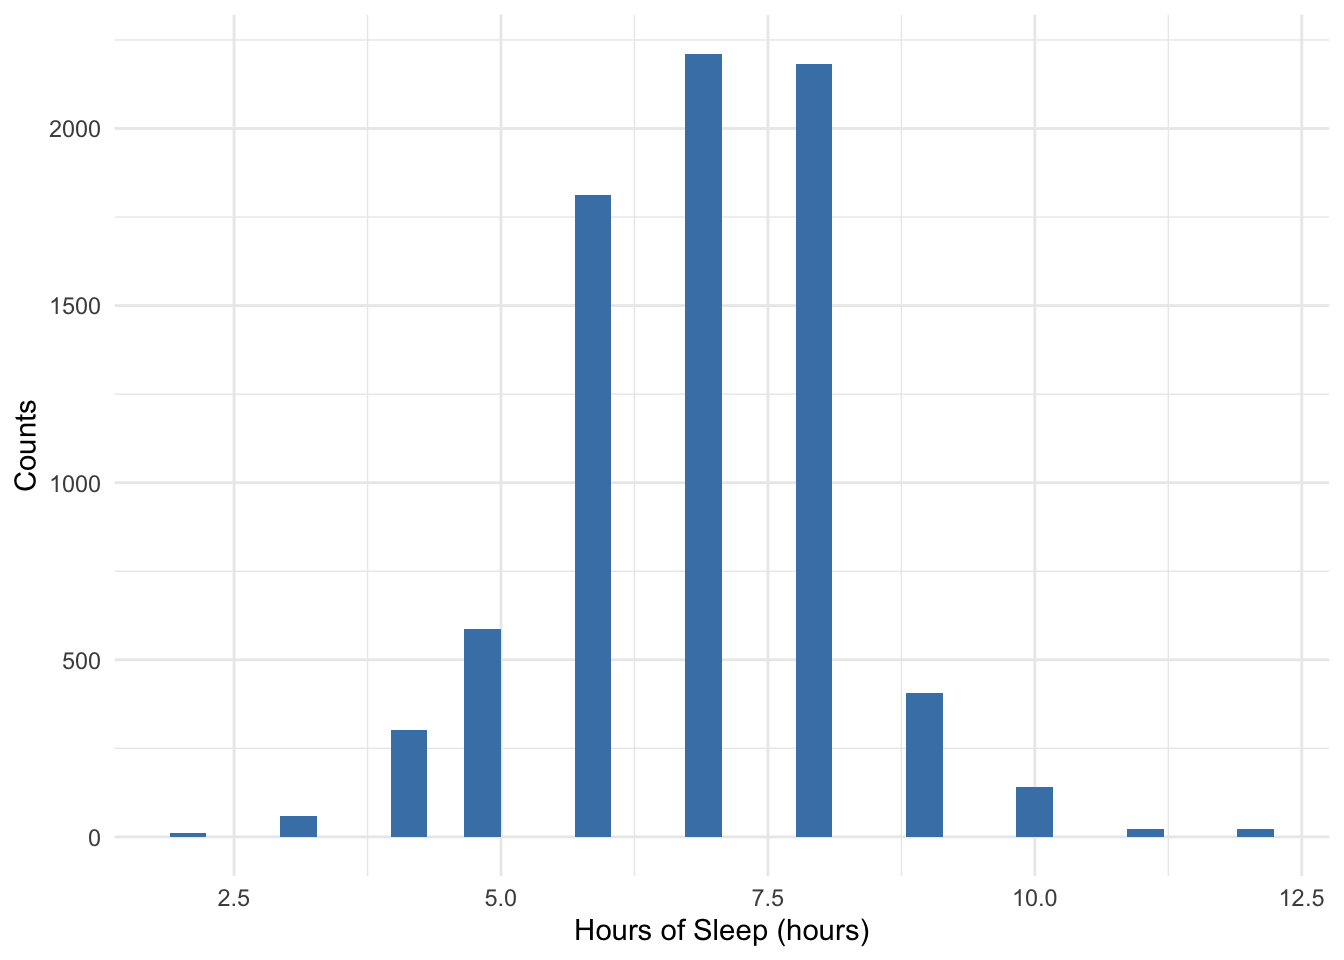
\includegraphics{02-visualization_files/figure-latex/unnamed-chunk-75-1.pdf}

\hypertarget{putting-everything-together}{%
\subsection{Putting everything together}\label{putting-everything-together}}

The combination of these different visual features can result in powerful visual understanding. Let's combine paneling with color information to explore if there are marital status patterns in these union-job sector subgroups.

\begin{Shaded}
\begin{Highlighting}[]
\NormalTok{CPS85 }\OperatorTok
\StringTok{    }\KeywordTok{ggplot}\NormalTok{(}\KeywordTok{aes}\NormalTok{(}\DataTypeTok{x =}\NormalTok{ educ, }\DataTypeTok{y =}\NormalTok{ wage, }\DataTypeTok{color =}\NormalTok{ married)) }\OperatorTok{+}
\StringTok{    }\KeywordTok{geom_point}\NormalTok{() }\OperatorTok{+}
\StringTok{    }\KeywordTok{geom_smooth}\NormalTok{(}\DataTypeTok{method =} \StringTok{'lm'}\NormalTok{) }\OperatorTok{+}
\StringTok{    }\KeywordTok{xlab}\NormalTok{(}\StringTok{"Years of education"}\NormalTok{) }\OperatorTok{+}
\StringTok{    }\KeywordTok{ylab}\NormalTok{(}\StringTok{"Hourly wage (US dollars)"}\NormalTok{) }\OperatorTok{+}
\StringTok{    }\KeywordTok{facet_grid}\NormalTok{(. }\OperatorTok{~}\StringTok{ }\NormalTok{sector) }\OperatorTok{+}\StringTok{ }
\StringTok{    }\KeywordTok{guides}\NormalTok{(}\DataTypeTok{color =} \KeywordTok{guide_legend}\NormalTok{(}\DataTypeTok{title =} \StringTok{"Marital status"}\NormalTok{)) }\OperatorTok{+}\StringTok{ }\CommentTok{# Legend title}
\StringTok{    }\KeywordTok{theme_minimal}\NormalTok{()}
\end{Highlighting}
\end{Shaded}

\begin{verbatim}
## `geom_smooth()` using formula 'y ~ x'
\end{verbatim}

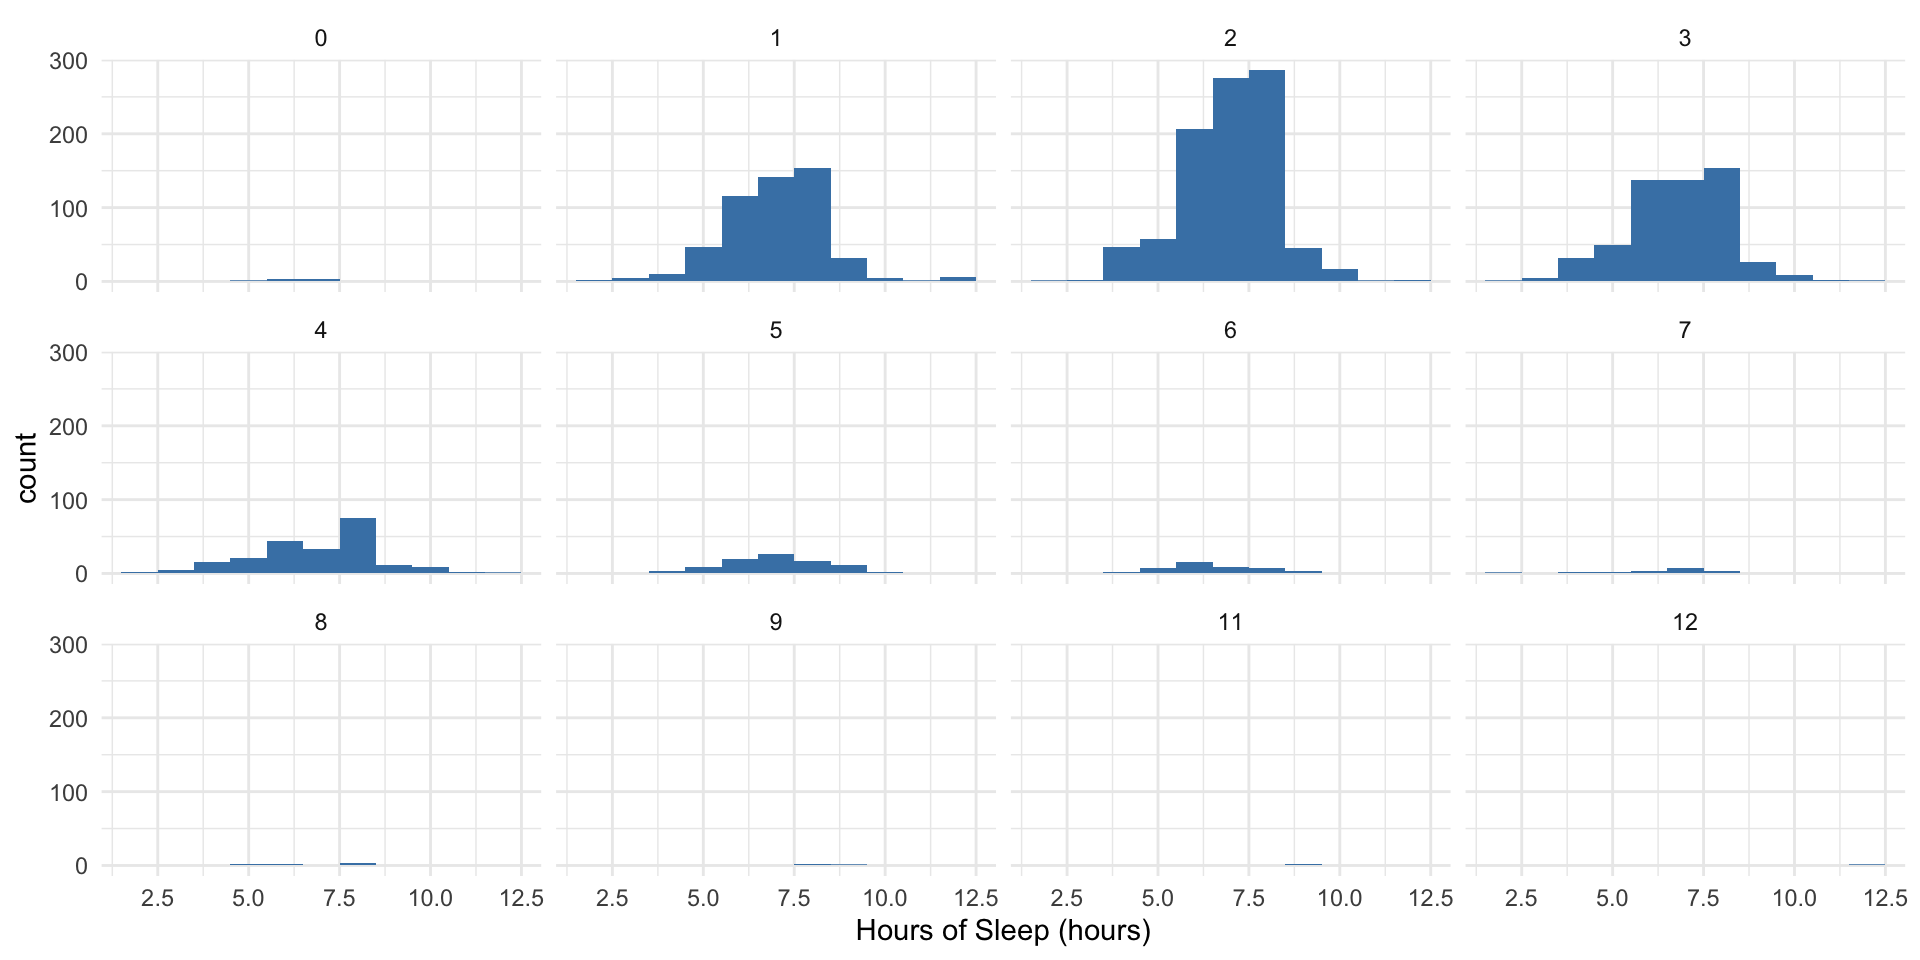
\includegraphics{02-visualization_files/figure-latex/unnamed-chunk-76-1.pdf}

Creating effective multivariate visualizations takes a lot of trial and error. Some visual elements will better highlight patterns than others, and often times, you'll have to try several iterations before you feel that you are learning something insightful from the graphic. Be tenacious, and keep in mind the good visualization principles outlined at the beginning of this chapter!

\hypertarget{chapter-2-major-takeaways}{%
\section{Chapter 2 Major Takeaways}\label{chapter-2-major-takeaways}}

\begin{enumerate}
\def\labelenumi{\arabic{enumi}.}
\item
  STOP: Think about whether a variable is categorical or quantitative. This informs the type of graphic and summaries that are appropriate.
\item
  The shape of a histogram tells you about the relationships between mean and median.
\item
  If you are describing a histogram, make sure to comment on the shape, center, spread, and outliers.
\item
  If you are describing a scatterplot, make sure to comment about the direction, form, strength, and unusual features.
\item
  Be vigilant for unusual points as they could be due to human error in the data collection, but do not automatically throw away unusual or outlying points. Think about whether they are feasible first.
\item
  Visualizations are just a starting place. Stop to notice what you learn and what questions you have about the data. Let that inform the next visualization you make.
\end{enumerate}

\hypertarget{linear-regression-models}{%
\chapter{Linear Regression Models}\label{linear-regression-models}}

In our visualizations of data, we've seen trends, patterns, and variation. Let's now endeavor to describe those trends, patterns, and variation more \emph{precisely} and \emph{quantitatively} by building statistical \emph{models}. In this chapter, we will focus on a class of models for describing quantitative outcome variables: linear regression models.

\hypertarget{modeling-goals}{%
\section{Modeling Goals}\label{modeling-goals}}

Broadly, a model is a simplified representation of the world. When we build models, we may have different goals.

One goal when building models is \textbf{prediction}. Given data on a \textbf{response} or \textbf{outcome variable}, \(Y\), and one or more \textbf{predictor or explanatory variables}, \(X\), the goal is to find a mathematical function, \(f\), of \(X\) that gives good predictions of \(Y\). For example, we might want to be able to predict a customer's chest size knowing their neck size. This \(X\) may be a single variable, but it is most often a set of variables. We'll be building up to multivariate modeling over the course of this chapter.

\begin{reflect}
Can you think of some other concrete examples in which we'd want a model
to do prediction? Consider what predictions might be made about you
every day.
\end{reflect}

What are the qualities of a good model and function, \(f\)? We want to find an \(f(X)\) such that if we plug in a value of \(X\) such as \(X=x\), we'll get a good predictor of the observed outcome values \(y\). In other words, we want the model prediction \(\hat{y}=f(x)\) (read, ``y hat'') to be close to the observed outcome value. We want \(y-\hat{y}\) to be small. This difference between the observed value and the prediction, \(y-\hat{y}\), is called a \textbf{residual}. We'll discuss residuals more later.

Another goal when building models is \textbf{description}. We want a model to ``explain'' the relationship between the \(X\) and \(Y\) variables. Note that an overly complicated model may not be that useful here because it can't help us \emph{understand} the relationship. A more complex model may, however, produce better predictions. \href{https://en.wikipedia.org/wiki/George_E._P._Box}{George Box} is often quoted ``All models are wrong but some are useful.'' Depending on our goal, one model may be more useful than another.

\begin{reflect}
Can you think of some concrete examples in which we'd want a model to do
explain a phenomenon? Consider how policy decisions get made.
\end{reflect}

To begin, we will consider a simple, but powerful model in which we limit this function, \(f(X)\), to be a straight line with a y-intercept, \(\beta_0\), and slope, \(\beta_1\). (\(\beta\) is the Greek letter beta.) The \(E[Y | X]\) below stands for the \textbf{expected value} of the response variable \(Y\) for a \emph{given} value of \(X\).

\[E[Y | X] = \beta_0 + \beta_1\,X\]

This is a \textbf{simple linear regression model}. We model the expected value (the average value) of the response variable given an explanatory variable \(X\) as a line. It is the foundation of many statistical models used in modern statistics and is more flexible than you may think.

We'll need to find the values of the slope and intercept that give us a line that gets close to the averages in order to explain the general relationship between \(X\) and \(Y\). We'll get to this soon.

Once we have values the intercept and slope, we are going to call them estimates and put a hat on them, so \(\hat{\beta}_0\) is our \textbf{estimated intercept} and our \textbf{estimated slope} is \(\hat{\beta}_1\). We can use those to make predictions by plugging in a value of x:

\[\hat{y} = \hat{\beta}_0 +\hat{\beta}_1 x\]

The little hat on top of \(\hat{y}\) means that we're talking about a predicted or estimated value of \(y\), so our model says that the predicted or estimated value of \(y\) is equal to an estimated intercept (\(\hat{\beta}_0\)), plus an estimated slope (\(\hat{\beta}_1\)), times the value \(x\).

\begin{mathbox}
In the past, you may have seen the equation of a line as

\[y = mx + b\]

where \(m\) is the slope and \(b\) is the y-intercept. We will be using
different notation so that it can generalize to multiple linear
regression.

The y-intercept is the value when \(x=0\) and the slope is change in
\(y\) for each 1 unit increase of \(x\) (``rise over run'').
\end{mathbox}

\hypertarget{lines}{%
\section{Lines}\label{lines}}

Let's return to the thought experiment in which you were a manufacturer of button-down dress shirts.

\begin{Shaded}
\begin{Highlighting}[]
\NormalTok{body <-}\StringTok{ }\KeywordTok{read.delim}\NormalTok{(}\StringTok{"Data/bodyfat.txt"}\NormalTok{)}

\NormalTok{body }\OperatorTok
\StringTok{    }\KeywordTok{ggplot}\NormalTok{(}\KeywordTok{aes}\NormalTok{(}\DataTypeTok{x =}\NormalTok{ Neck, }\DataTypeTok{y =}\NormalTok{ Chest)) }\OperatorTok{+}
\StringTok{    }\KeywordTok{geom_point}\NormalTok{(}\DataTypeTok{color =} \StringTok{'steelblue'}\NormalTok{) }\OperatorTok{+}\StringTok{ }
\StringTok{    }\KeywordTok{xlab}\NormalTok{(}\StringTok{'Neck size (cm)'}\NormalTok{) }\OperatorTok{+}\StringTok{ }
\StringTok{    }\KeywordTok{ylab}\NormalTok{(}\StringTok{'Chest size (cm)'}\NormalTok{) }\OperatorTok{+}
\StringTok{    }\KeywordTok{theme_minimal}\NormalTok{()}
\end{Highlighting}
\end{Shaded}

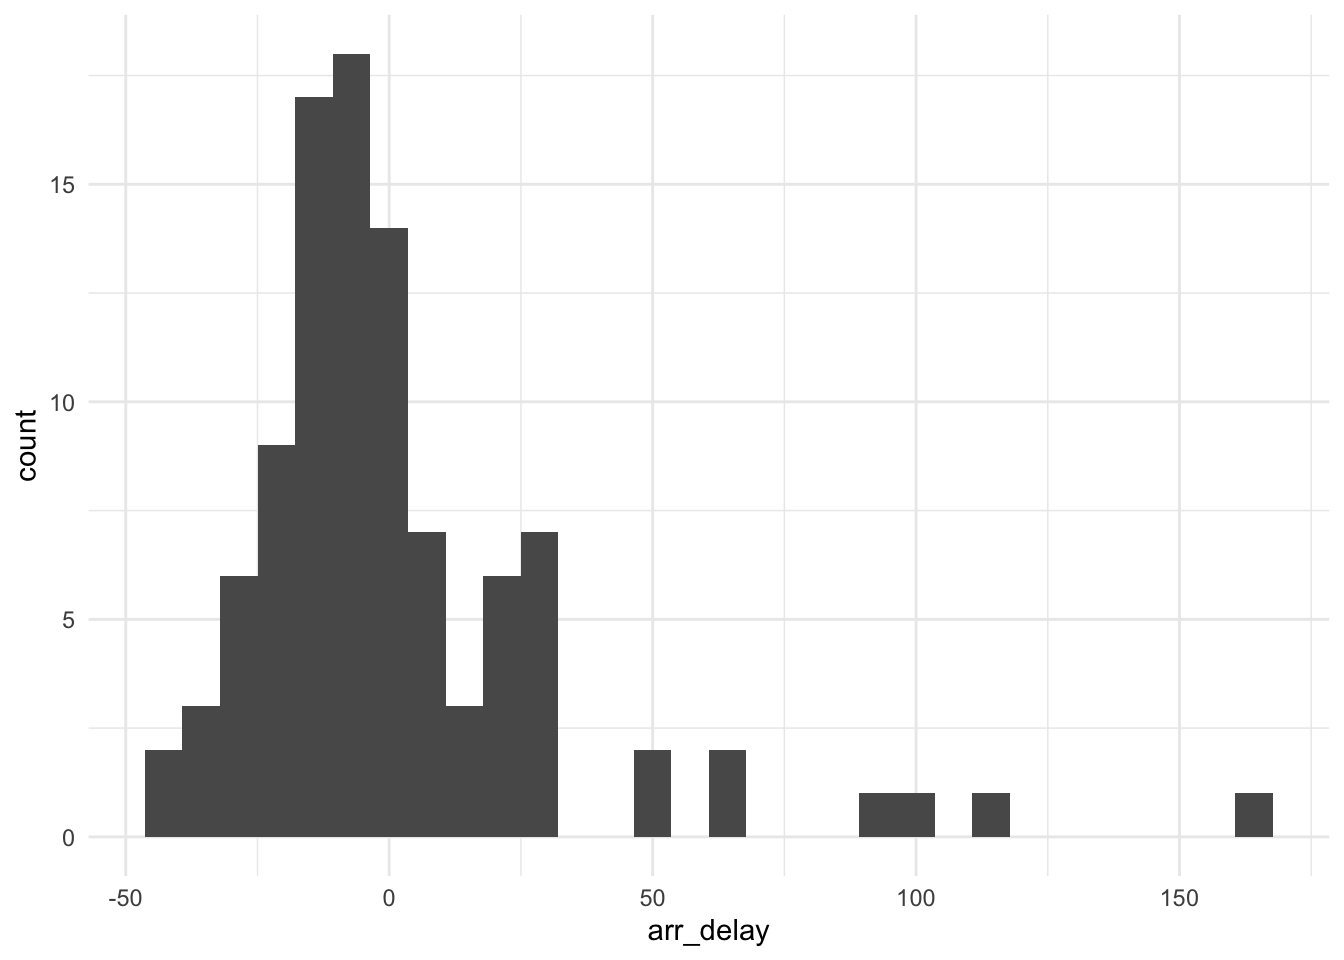
\includegraphics{03-linear-regression_files/figure-latex/unnamed-chunk-4-1.pdf}

\begin{reflect}
If you were to add one or multiple lines to the plot above to help you
make business decisions, where would you want it (or them)?
\end{reflect}

Let's say you were only going to make one size of shirt. You might want to add a horizontal line at the mean Chest size and a vertical line at the mean Neck size.

\begin{Shaded}
\begin{Highlighting}[]
\NormalTok{body }\OperatorTok
\StringTok{    }\KeywordTok{ggplot}\NormalTok{(}\KeywordTok{aes}\NormalTok{(}\DataTypeTok{x =}\NormalTok{ Neck, }\DataTypeTok{y =}\NormalTok{ Chest)) }\OperatorTok{+}
\StringTok{    }\KeywordTok{geom_point}\NormalTok{(}\DataTypeTok{color =} \StringTok{'steelblue'}\NormalTok{) }\OperatorTok{+}\StringTok{ }
\StringTok{    }\KeywordTok{geom_hline}\NormalTok{(}\DataTypeTok{yintercept =} \KeywordTok{mean}\NormalTok{(body}\OperatorTok{$}\NormalTok{Chest)) }\OperatorTok{+}
\StringTok{    }\KeywordTok{geom_vline}\NormalTok{(}\DataTypeTok{xintercept =} \KeywordTok{mean}\NormalTok{(body}\OperatorTok{$}\NormalTok{Neck)) }\OperatorTok{+}
\StringTok{    }\KeywordTok{xlab}\NormalTok{(}\StringTok{'Neck size (cm)'}\NormalTok{) }\OperatorTok{+}\StringTok{ }
\StringTok{    }\KeywordTok{ylab}\NormalTok{(}\StringTok{'Chest size (cm)'}\NormalTok{) }\OperatorTok{+}
\StringTok{    }\KeywordTok{theme_minimal}\NormalTok{()}
\end{Highlighting}
\end{Shaded}

\includegraphics{03-linear-regression_files/figure-latex/unnamed-chunk-6-1.pdf}

We can see that a shirt made to these specifications would fit the ``average person.'' However, this might not serve your market very well. For many people, the shirt would be too tight because their chest and/or neck sizes would be larger than average. For many people, the shirt would be too large because they chest and/or neck sizes would be smaller than average.

Let's try something else. Let's allow ourselves 5 different sizes (XS, S, M, L, XL). Then, we can cut the neck size variable into 5 groups of equal length and estimate the mean chest sizes within each of these groups.

\includegraphics{03-linear-regression_files/figure-latex/unnamed-chunk-7-1.pdf}

\begin{reflect}
What do these lines tell us for our business venture?
\end{reflect}

What if we wanted to be able to make more sizes? Could we get a pretty good sense of what the chest sizes should be for a given neck size? Let's try allowing for 8 different sizes.

\includegraphics{03-linear-regression_files/figure-latex/unnamed-chunk-9-1.pdf}

\begin{reflect}
What are the pros and cons of having a larger number of sizes?
\end{reflect}

\begin{reflect}
Stop and think about the data collection process. If you were measuring
your own neck size, how precise do you think you could get? What factors
might impact that precision?
\end{reflect}

We can see from this scatterplot that there is generally a linear relationship between neck and chest size. Perhaps we can find one line to describe the relationship between neck size and chest size and use that line to decide on sizes later.

\includegraphics{03-linear-regression_files/figure-latex/unnamed-chunk-12-1.pdf}

\begin{reflect}
What does line tell us for our business venture?
\end{reflect}

If the scatterplot between two quantitative variables \textbf{resembles a straight line},

\begin{itemize}
\tightlist
\item
  a straight line could roughly \textbf{describe} the mean or average value of \(y\) for each value of \(x\).
\item
  a straight line could \textbf{describe} how much we'd \emph{expect} \(y\) to change based on a 1 unit change in \(x\).
\item
  a straight line could help us \textbf{predict} the \(y\) based on a new value of \(x\).
\end{itemize}

\hypertarget{best-fitting-line}{%
\section{``Best'' fitting line}\label{best-fitting-line}}

To choose the ``best'' fitting line, we need to find estimates of the intercept (\(\beta_0\)) and slope (\(\beta_1\)),

\[ E[Y | X] =  \beta_0 + \beta_1\,X \]

that gives us the ``best'' fit to the \(n\) points on a scatterplot, \((x_i,y_i)\) where \(i=1,...,n\).

\begin{reflect}
What do we mean by ``best''? In general, we'd like good predictions and
a model that describes the average relationship. But we need to be more
precise about what we mean by ``best''.
\end{reflect}

\hypertarget{first-idea}{%
\subsection{First idea}\label{first-idea}}

One idea of ``best'' is that we want the line that minimizes the sum of the \textbf{residuals}, \(e_i = y_i - \hat{y}_i = y_i - ( \hat{\beta}_0 + \hat{\beta}_1x_i)\). The residual is the error in our prediction, the difference between what you observe and what you predict based on the line.

\begin{itemize}
\tightlist
\item
  \textbf{Problem}: We will have positive and negative residuals; they will cancel each other out if we add them together. While a good idea, this definition of ``best'' won't give us what we want. We'll want an idea that deals with the negative signs.
\end{itemize}

\hypertarget{second-idea}{%
\subsection{Second idea}\label{second-idea}}

Another idea of ``best'' is that we want the line that minimizes the sum of the absolute value of the residuals, \(\sum_{i=1}^n |y_i - \hat{y}_i| = \sum_{i=1}^n |y_i - ( \hat{\beta}_0 + \hat{\beta}_1x_i)| = \sum_{i=1}^n |e_i|\).

\begin{itemize}
\tightlist
\item
  \textbf{Problem}: This definition of ``best'' results in a procedure referred to as \textbf{Least Absolute Deviations}, but there isn't always one unique line that satisfies this. So, while this is a valid definition of ``best,'' this isn't stable as there isn't always one ``best'' line.
\end{itemize}

\hypertarget{third-idea}{%
\subsection{Third idea}\label{third-idea}}

Lastly, another idea of ``best'' is that we want the line that minimizes the sum of squared residuals, \(\sum_{i=1}^n (y_i - \hat{y}_i)^2= \sum_{i=1}^n(y_i-( \hat{\beta}_0 + \hat{\beta}_1x_i))^2=\sum_{i=1}^n e_i^2\).

\begin{itemize}
\tightlist
\item
  This is referred to as \textbf{Least Squares} and has a unique solution. We'll will focus on this definition of ``best'' in this class. It also has some really nice mathematical properties and \href{https://medium.com/@andrew.chamberlain/the-linear-algebra-view-of-least-squares-regression-f67044b7f39b}{connections to linear algebra}.
\end{itemize}

\hypertarget{least-squares}{%
\section{Least Squares}\label{least-squares}}

Let's try to find the line that \textbf{minimizes the Sum of Squared Residuals} by searching over a grid of values for (intercept, slope).

Below is a visual of the sum of squared residuals for a variety of values of the intercept and slope. The surface height is sum of squared residuals for each combination of slope and intercept.

\includegraphics{03-linear-regression_files/figure-latex/unnamed-chunk-15-1.pdf}

We can see there is valley where the minimum must be. Let's visualize this in a slightly different way. We'll encode the surface height as color (white is lowest).

\includegraphics{03-linear-regression_files/figure-latex/unnamed-chunk-16-1.pdf}

The large values of the sum of squared residuals are dominating this image, so let's change the color scheme to see more variation in smaller values (white is lowest).

\includegraphics{03-linear-regression_files/figure-latex/unnamed-chunk-17-1.pdf}

We can limit our search to \(\beta_0 \in (-10,10)\) and \(\beta_1 \in (2,3)\).

\begin{Shaded}
\begin{Highlighting}[]
\NormalTok{beta0 <-}\StringTok{ }\KeywordTok{seq}\NormalTok{(}\OperatorTok{-}\DecValTok{10}\NormalTok{, }\DecValTok{10}\NormalTok{, }\DataTypeTok{by =} \FloatTok{0.05}\NormalTok{)}
\NormalTok{beta1 <-}\StringTok{ }\KeywordTok{seq}\NormalTok{(}\DecValTok{2}\NormalTok{, }\DecValTok{3}\NormalTok{, }\DataTypeTok{by =} \FloatTok{0.05}\NormalTok{)}
\NormalTok{b <-}\StringTok{ }\KeywordTok{expand.grid}\NormalTok{(beta0,beta1)}
\NormalTok{ss <-}\StringTok{ }\KeywordTok{apply}\NormalTok{(b,}\DecValTok{1}\NormalTok{,f)}

\NormalTok{b[ss }\OperatorTok{==}\StringTok{ }\KeywordTok{min}\NormalTok{(ss),]}
\end{Highlighting}
\end{Shaded}

\begin{verbatim}
##      Var1 Var2
## 6142 -3.7 2.75
\end{verbatim}

We have the minimum point. Over the grid of pairs of values, the minimum sum of squared residuals happens when the intercept is -3.7 and the slope is 2.75.

\begin{mathbox}
(Optional) Alternative ways (faster than exhaustive search) to find the
minimum sum of squared residuals:

\begin{itemize}
\tightlist
\item
  We could try a numerical optimization algorithm such as steepest
  descent.
\item
  We could use multivariable calculus (find partial derivatives, set
  equal to 0, and solve).
\end{itemize}

To get started on the calculus, solve the following two equations for
the two unknowns (\(\beta_0\) and \(\beta_1\)):

\[\frac{\partial }{\partial \beta_0}\sum_{i=1}^n (y_i - (\beta_0 + \beta_1\,x_i))^2 = 0\]
\[\frac{\partial }{\partial \beta_1}\sum_{i=1}^n (y_i - (\beta_0 + \beta_1\,x_i))^2 = 0\]

If you are a math/stat/physics/cs major, you should try this by hand and
see if you can get the solutions below.
\end{mathbox}

If you find the minimum using calculus (super useful class!), you'll find that we can write the Least Squares solution in an equation format as functions of summary statistics (!), the estimated slope is

\[ \hat{\beta}_1  = r\frac{s_y}{s_x}\]

and the estimated intercept is

\[ \hat{\beta}_0 = \bar{y} - \hat{\beta}_1\bar{x} \]

where \(\bar{x}\) is the mean of the variable on the x-axis, \(\bar{y}\) is the mean of the variable on the y-axis, \(s_x\) is the standard deviation of the variable on the x-axis, \(s_y\) is the standard deviation of the variable on the y-axis, and \(r\) is the correlation coefficient between the two variables.

Let's do that calculation ``by hand'' first in R.

\begin{Shaded}
\begin{Highlighting}[]
\NormalTok{body }\OperatorTok
\StringTok{    }\KeywordTok{summarize}\NormalTok{(}\DataTypeTok{sy =} \KeywordTok{sd}\NormalTok{(Chest), }\DataTypeTok{sx =} \KeywordTok{sd}\NormalTok{(Neck), }\DataTypeTok{r =} \KeywordTok{cor}\NormalTok{(Chest,Neck), }\DataTypeTok{ybar =} \KeywordTok{mean}\NormalTok{(Chest), }\DataTypeTok{xbar =} \KeywordTok{mean}\NormalTok{(Neck)) }\OperatorTok
\StringTok{    }\KeywordTok{mutate}\NormalTok{(}\DataTypeTok{beta1 =}\NormalTok{ r}\OperatorTok{*}\NormalTok{sy}\OperatorTok{/}\NormalTok{sx, }\DataTypeTok{beta0 =}\NormalTok{ ybar }\OperatorTok{-}\StringTok{ }\NormalTok{beta1}\OperatorTok{*}\NormalTok{xbar) }\OperatorTok
\StringTok{    }\KeywordTok{select}\NormalTok{(beta0, beta1)}
\end{Highlighting}
\end{Shaded}

\begin{verbatim}
##       beta0    beta1
## 1 -3.188483 2.736883
\end{verbatim}

Wow. That was quite a bit of coding. From now on, we'll take the shortcut and use the \texttt{lm()} function which stands for \textbf{l}inear \textbf{m}odel. This function gives us the least squares solution to the ``best'' fitting line, as defined by minimizing the sum of squared residuals.

\begin{Shaded}
\begin{Highlighting}[]
\NormalTok{body }\OperatorTok\StringTok{ }\KeywordTok{with}\NormalTok{(}\KeywordTok{lm}\NormalTok{(Chest }\OperatorTok{~}\StringTok{ }\NormalTok{Neck)) }\CommentTok{# When you see ~, think "as a function of"}
\end{Highlighting}
\end{Shaded}

\begin{verbatim}
## 
## Call:
## lm(formula = Chest ~ Neck)
## 
## Coefficients:
## (Intercept)         Neck  
##      -3.188        2.737
\end{verbatim}

\begin{Shaded}
\begin{Highlighting}[]
\CommentTok{#or you can use the following code:}
\CommentTok{#lm(Chest ~ Neck, data = body)}
\end{Highlighting}
\end{Shaded}

\hypertarget{properties-of-least-squares-line}{%
\section{Properties of Least Squares Line}\label{properties-of-least-squares-line}}

\begin{itemize}
\item
  \((\bar{x},\bar{y})\) is ALWAYS on the least squares line.
\item
  The residuals from the least squares line ALWAYS sum to 0.
\item
  The mean of the residuals from the least squares line is ALWAYS 0.
\item
  The \textbf{standard deviation of the residuals,} \(s_e\), gives us a sense of how bad our predictions (based on the line) could be. In other words, it gives us a sense of the size of our prediction errors:
\end{itemize}

\[s_e = \sqrt{\frac{\sum^n_{i=1} (y_i-\hat{y}_i)^2}{n-2}}  = \sqrt{\frac{\sum^n_{i=1} (e_i-0)^2}{n-2}} \]

In R: the standard deviation of the residuals, \(s_e\), is referred to as the ``residual standard error''. Don't confuse this with ``Std. Error,'' which is something else that we'll get to later in the semester.

\begin{Shaded}
\begin{Highlighting}[]
\NormalTok{body }\OperatorTok
\StringTok{    }\KeywordTok{with}\NormalTok{(}\KeywordTok{lm}\NormalTok{(Chest }\OperatorTok{~}\StringTok{ }\NormalTok{Neck)) }\OperatorTok\StringTok{ }
\StringTok{    }\KeywordTok{summary}\NormalTok{()}
\end{Highlighting}
\end{Shaded}

\begin{verbatim}
## 
## Call:
## lm(formula = Chest ~ Neck)
## 
## Residuals:
##      Min       1Q   Median       3Q      Max 
## -15.1447  -3.3328  -0.5342   3.0738  16.5974 
## 
## Coefficients:
##             Estimate Std. Error t value Pr(>|t|)    
## (Intercept)  -3.1885     5.4951   -0.58    0.562    
## Neck          2.7369     0.1446   18.93   <2e-16 ***
## ---
## Signif. codes:  0 '***' 0.001 '**' 0.01 '*' 0.05 '.' 0.1 ' ' 1
## 
## Residual standard error: 5.225 on 248 degrees of freedom
## Multiple R-squared:  0.5911,	Adjusted R-squared:  0.5894 
## F-statistic: 358.5 on 1 and 248 DF,  p-value: < 2.2e-16
\end{verbatim}

This fit simple linear regression line is

\[ \widehat{\hbox{Chest}} = -3.18 + 2.73\,\hbox{Neck}\]

If you have a neck size of 38 cm, then we predict the chest size of an ideal shirt is about 100.5 cm:

\begin{Shaded}
\begin{Highlighting}[]
\CommentTok{# The intercept and slope are rounded here first (not great):}
\FloatTok{-3.18} \OperatorTok{+}\StringTok{ }\FloatTok{2.73}\OperatorTok{*}\DecValTok{38}
\end{Highlighting}
\end{Shaded}

\begin{verbatim}
## [1] 100.56
\end{verbatim}

\begin{Shaded}
\begin{Highlighting}[]
\CommentTok{# The intercept and slope are not rounded before prediction (better!)}
\NormalTok{body }\OperatorTok
\StringTok{    }\KeywordTok{with}\NormalTok{(}\KeywordTok{lm}\NormalTok{(Chest }\OperatorTok{~}\StringTok{ }\NormalTok{Neck)) }\OperatorTok\StringTok{ }
\StringTok{    }\KeywordTok{predict}\NormalTok{(}\DataTypeTok{newdata =} \KeywordTok{data.frame}\NormalTok{(}\DataTypeTok{Neck =} \DecValTok{38}\NormalTok{))}
\end{Highlighting}
\end{Shaded}

\begin{verbatim}
##        1 
## 100.8131
\end{verbatim}

Given your neck size, we can probably predict your chest size within 5 to 10 cm since \(s_e = 5.22\) (1 to 2 SD's -- recall Section \ref{intro-zscore}).

\begin{reflect}
If you were a shirt manufacturer, is this a good enough prediction? What
is the impact on the customer? Think of if the prediction were an
overestimate (loose) or an underestimate (too tight).
\end{reflect}

\hypertarget{real-companies}{%
\subsection{Real companies}\label{real-companies}}

Let's see how some real companies create shirts. In the plots below, the red boxes represent the advertised range (in cm) for Neck and Chest sizes for each brand.

\includegraphics[width=.25\textwidth]{Photos/shirtchart}

For Calvin Klein, we see that the red boxes are below the least squares line (black line). So for a given neck size, Calvin Klein makes shirts that are a little bit too small at the chest.

\includegraphics{03-linear-regression_files/figure-latex/unnamed-chunk-26-1.pdf}

For Express, we see that the red boxes are generally on the least squares line, except for the smallest size. This means that Express shirts are generally a good fit at the chest and neck for the 4 largest sizes, but the smallest shirt size is a bit too small at the chest for the neck size.

\includegraphics{03-linear-regression_files/figure-latex/unnamed-chunk-27-1.pdf}

For Brooks Brothers, the red boxes are a bit below the least squares line for the 3 smallest sizes and a little above the line for the largest size. This means that the 3 smallest sizes are a bit too small in the chest for our customers (in our data set) with those neck sizes and that the largest shirt is a bit big at the chest for that neck size.

\includegraphics{03-linear-regression_files/figure-latex/unnamed-chunk-28-1.pdf}

\begin{reflect}
We haven't told you how the customer data we've been using was
collected. As you compared the brand sizes to this sample data, what
assumptions were you making about the population that the sample was
drawn from?

What questions do you have about the sampling procedure?
\end{reflect}

\hypertarget{model-interpretation}{%
\section{Model Interpretation}\label{model-interpretation}}

Let's look at the summary output of the \texttt{lm()} function in R again. We'll highlight some of the most important pieces of this output and discuss how you interpret them.

\begin{Shaded}
\begin{Highlighting}[]
\NormalTok{tshirt_mod <-}\StringTok{ }\KeywordTok{lm}\NormalTok{(Chest }\OperatorTok{~}\StringTok{ }\NormalTok{Neck, }\DataTypeTok{data =}\NormalTok{ body)}
\KeywordTok{summary}\NormalTok{(tshirt_mod)}
\end{Highlighting}
\end{Shaded}

\begin{verbatim}
## 
## Call:
## lm(formula = Chest ~ Neck, data = body)
## 
## Residuals:
##      Min       1Q   Median       3Q      Max 
## -15.1447  -3.3328  -0.5342   3.0738  16.5974 
## 
## Coefficients:
##             Estimate Std. Error t value Pr(>|t|)    
## (Intercept)  -3.1885     5.4951   -0.58    0.562    
## Neck          2.7369     0.1446   18.93   <2e-16 ***
## ---
## Signif. codes:  0 '***' 0.001 '**' 0.01 '*' 0.05 '.' 0.1 ' ' 1
## 
## Residual standard error: 5.225 on 248 degrees of freedom
## Multiple R-squared:  0.5911,	Adjusted R-squared:  0.5894 
## F-statistic: 358.5 on 1 and 248 DF,  p-value: < 2.2e-16
\end{verbatim}

\hypertarget{intercept-hatbeta_0}{%
\subsection{\texorpdfstring{Intercept (\(\hat{\beta}_0\))}{Intercept (\textbackslash hat\{\textbackslash beta\}\_0)}}\label{intercept-hatbeta_0}}

\begin{itemize}
\tightlist
\item
  \textbf{Where to find:} In the table called ``Coefficients'', look for the number under ``Estimate'' for ``(Intercept)''. It is -3.1885 for this model.
\item
  \textbf{Definition:} The intercept gives the average value of \(y\) when \(x=0\) (\textbf{think about context})
\item
  \textbf{Interpretation:} If Neck size = 0, then the person doesn't exist. In this context, the intercept doesn't make much sense to interpret.
\item
  \textbf{Discussion:} If the intercept doesn't make sense in the context, we might refit the model with the \(x\) variable once it is \textbf{centered}. That is, the mean of \(x\) for all individuals in the sample is computed, and this mean is subtracted from each person's \(x\) value. In this case, the intercept is interpreted as the average value of \(y\) when \(x\) is at its (sample) mean value. See the example below -- we get an intercept of 100.66, which is the average Chest size for customers with average Neck size. We could also choose to center Neck size at a value other than the mean. For example, we could center it at 30 cm by subtracting 30 from the Neck size of all cases.
\end{itemize}

\begin{Shaded}
\begin{Highlighting}[]
\NormalTok{body <-}\StringTok{ }\NormalTok{body }\OperatorTok\StringTok{ }\KeywordTok{mutate}\NormalTok{(}\DataTypeTok{CNeck =}\NormalTok{ Neck }\OperatorTok{-}\StringTok{ }\KeywordTok{mean}\NormalTok{(Neck))}
\NormalTok{tshirt_mod2 <-}\StringTok{ }\KeywordTok{lm}\NormalTok{(Chest }\OperatorTok{~}\StringTok{ }\NormalTok{CNeck, }\DataTypeTok{data =}\NormalTok{ body)}
\KeywordTok{summary}\NormalTok{(tshirt_mod2)}
\end{Highlighting}
\end{Shaded}

\begin{verbatim}
## 
## Call:
## lm(formula = Chest ~ CNeck, data = body)
## 
## Residuals:
##      Min       1Q   Median       3Q      Max 
## -15.1447  -3.3328  -0.5342   3.0738  16.5974 
## 
## Coefficients:
##             Estimate Std. Error t value Pr(>|t|)    
## (Intercept) 100.6620     0.3304  304.63   <2e-16 ***
## CNeck         2.7369     0.1446   18.93   <2e-16 ***
## ---
## Signif. codes:  0 '***' 0.001 '**' 0.01 '*' 0.05 '.' 0.1 ' ' 1
## 
## Residual standard error: 5.225 on 248 degrees of freedom
## Multiple R-squared:  0.5911,	Adjusted R-squared:  0.5894 
## F-statistic: 358.5 on 1 and 248 DF,  p-value: < 2.2e-16
\end{verbatim}

\hypertarget{slope-hatbeta_1}{%
\subsection{\texorpdfstring{Slope (\(\hat{\beta}_1\))}{Slope (\textbackslash hat\{\textbackslash beta\}\_1)}}\label{slope-hatbeta_1}}

\begin{itemize}
\tightlist
\item
  \textbf{Where to find:} In the table called ``Coefficients'', look for the number under ``Estimate'' for the name of the variable, ``Neck'' or ``CNeck''. It is 2.7369 for this model. (Note: the slopes for both \texttt{tshirt\_mod} and \texttt{tshirt\_mod2} are the same. Why?)
\item
  \textbf{Definition:} The slope gives the change in average \(y\) per 1 unit increase in \(x\) (\textbf{not for individuals and not a causal statement})
\item
  \textbf{One Interpretation:} If we compare two groups of individuals with a 1 cm difference in the neck size (e.g., 38 cm and 39 cm OR 40 cm and 41 cm), then we'd expect the average chest sizes to be different by about 2.7 cm.
\item
  \textbf{Another Interpretation:} We'd expect the average chest size to increase by about 2.7 cm for each centimeter increase in neck size.
\item
  \textbf{A Third Interpretation:} We estimate that a one centimeter increase in neck size is associated with an increase, on average, of 2.7 cm in chest size.
\item
  \textbf{Discussion:} Note that the interpretations are not written about an individual because the least squares line (our fit model) is a description of the \textbf{general trend} in the population. The slope describes the change in the average, not the change for one person.
\end{itemize}

\hypertarget{least-squares-regression-line-haty-hatbeta_0-hatbeta_1x}{%
\subsection{\texorpdfstring{Least Squares Regression Line (\(\hat{y} = \hat{\beta}_0 + \hat{\beta}_1x\))}{Least Squares Regression Line (\textbackslash hat\{y\} = \textbackslash hat\{\textbackslash beta\}\_0 + \textbackslash hat\{\textbackslash beta\}\_1x)}}\label{least-squares-regression-line-haty-hatbeta_0-hatbeta_1x}}

\begin{itemize}
\tightlist
\item
  \textbf{Where to find:} In the table called ``Coefficients'', all of the values that you need to write down the formula of the line are in the ``Estimate'' column.
\item
  \textbf{Definition:} The line gives the estimated average of \(y\) for each value of \(x\) (\textbf{within the observed range of x})
\item
  \textbf{Interpretation:} The fit regression line of (Predicted Chest = -3.18 + 2.73*Neck) gives the estimated average Chest size for a given Neck size, based on our sample of data.
\item
  \textbf{Discussion:} The ``within the observed range of \(x\)'' phrase is very important. We can't predict values of \(y\) for values of \(x\) that are very different from what we have in our data. Trying to do so is a big no-no called \textbf{extrapolation}. We'll discuss this more in a bit.
\end{itemize}

\hypertarget{correlation-vs.-causation}{%
\subsection{Correlation vs.~Causation}\label{correlation-vs.-causation}}

\includegraphics{Photos/correlation.png}
Source: \href{https://xkcd.com/552/}{xkcd}

What is causation? What is a causal effect? Are there criteria for defining a cause?

These are deep questions that have been debated by scientists of all domains for a long time. We are at a point now where there is some consensus on the definition of a causal effect. The causal effect of a variable \(X\) on another variable \(Y\) is the amount that we expect \(Y\) to change if we \textbf{intervene on or manipulate} \(X\) by changing it by one unit.

When can we interpret an estimated slope, \(\hat{\beta}_1\), from a simple linear regression as a causal effect of \(X\) on \(Y\)? Well, in the simple linear regression case, almost never. To interpret the slope as a causal effect, there would have to be \textbf{no confounding variables} (no variables that cause \textbf{both} \(X\) \textbf{and} \(Y\)). If we performed an experiment, it might be possible to have no confounding variables, but in most situations, this is not feasible.

Then what are we to do?

\begin{enumerate}
\def\labelenumi{\arabic{enumi}.}
\tightlist
\item
  Think about the possible causal pathways and try and create a DAG (coming up - see Section \ref{dag}).
\item
  Try to \textbf{adjust or control for} possible confounders using multiple linear regression by including them in the model (coming up - see Section \ref{multiple}).
\item
  After fitting a model, we should step back and consider other criteria such as \href{https://en.wikipedia.org/wiki/Bradford_Hill_criteria}{Hill's Criteria} before concluding there is a cause and effect relationship. Think about whether there is a large effect, whether it can be reproduced in another sample, whether the the effect happens before the cause in time, etc.
\end{enumerate}

\hypertarget{model-evaluation}{%
\section{Model Evaluation}\label{model-evaluation}}

In this section, we consider model evaluation. We seek to develop tools that allow us to answer: is this a ``good'' model?

Aligning with our goals, we'd like to the model to:

\begin{itemize}
\tightlist
\item
  have small prediction errors
\item
  accurately capture the relationship that explains variation in the outcome
\end{itemize}

\hypertarget{prediction}{%
\subsection{Prediction}\label{prediction}}

Let's consider another data example. Can we predict your college grade point average (GPA) based on your high school GPA? (Disclaimer: this is not Macalester data)

\begin{Shaded}
\begin{Highlighting}[]
\NormalTok{sat <-}\StringTok{ }\KeywordTok{read_csv}\NormalTok{(}\StringTok{"Data/sat.csv"}\NormalTok{)}
\end{Highlighting}
\end{Shaded}

\begin{Shaded}
\begin{Highlighting}[]
\NormalTok{sat }\OperatorTok
\StringTok{    }\KeywordTok{ggplot}\NormalTok{(}\KeywordTok{aes}\NormalTok{(}\DataTypeTok{x =}\NormalTok{ high_GPA, }\DataTypeTok{y =}\NormalTok{ univ_GPA)) }\OperatorTok{+}
\StringTok{    }\KeywordTok{geom_point}\NormalTok{(}\DataTypeTok{color =} \StringTok{'steelblue'}\NormalTok{) }\OperatorTok{+}
\StringTok{    }\KeywordTok{geom_smooth}\NormalTok{(}\DataTypeTok{method =} \StringTok{'lm'}\NormalTok{, }\DataTypeTok{se =} \OtherTok{FALSE}\NormalTok{) }\OperatorTok{+}
\StringTok{    }\KeywordTok{xlab}\NormalTok{(}\StringTok{'High School GPA'}\NormalTok{) }\OperatorTok{+}
\StringTok{    }\KeywordTok{ylab}\NormalTok{(}\StringTok{'College GPA'}\NormalTok{) }\OperatorTok{+}\StringTok{ }
\StringTok{    }\KeywordTok{theme_minimal}\NormalTok{()}
\end{Highlighting}
\end{Shaded}

\includegraphics{03-linear-regression_files/figure-latex/unnamed-chunk-33-1.pdf}

First things first. Let's describe the scatterplot.

\begin{itemize}
\tightlist
\item
  \textbf{Direction}: Positive relationship (higher high school GPA is associated with higher college GPA)
\item
  \textbf{Form}: Roughly linear
\item
  \textbf{Strength}: There is a weak relationship when high school GPA \textless{} 3.0 (\(r = 0.32\)) and a fairly strong relationship when high school GPA \textgreater{} 3.0 (\(r = 0.68\)).
\item
  \textbf{Unusual}: As seen with the strength, there is greater variability in college GPA among individuals with lower high school GPA. That variability decreases with increased high school GPA. We call this pattern of unequal variation as \textbf{``thickening''} or \textbf{heteroscedasticity} (this term is used quite a bit in Econometrics).
\end{itemize}

The code below computes the correlation coefficients separately for students with high school GPAs above 3 and for students with high school GPAs less than or equal to 3. We see that the correlation is higher for the high GPA group.

\begin{Shaded}
\begin{Highlighting}[]
\NormalTok{sat }\OperatorTok
\StringTok{    }\KeywordTok{mutate}\NormalTok{(}\DataTypeTok{HighHSGPA =}\NormalTok{ high_GPA }\OperatorTok{>}\StringTok{ }\DecValTok{3}\NormalTok{) }\OperatorTok
\StringTok{    }\KeywordTok{group_by}\NormalTok{(HighHSGPA) }\OperatorTok
\StringTok{    }\KeywordTok{summarize}\NormalTok{(}\DataTypeTok{Cor =} \KeywordTok{cor}\NormalTok{(high_GPA,univ_GPA))}
\end{Highlighting}
\end{Shaded}

\begin{verbatim}
## # A tibble: 2 x 2
##   HighHSGPA   Cor
##   <lgl>     <dbl>
## 1 FALSE     0.316
## 2 TRUE      0.687
\end{verbatim}

Let's build a model to predict college GPA based on high school GPA based on this sample data. Since we noted that there was a linear relationship, let's fit a linear model by finding the least squares regression line.

\begin{Shaded}
\begin{Highlighting}[]
\NormalTok{sat }\OperatorTok
\StringTok{  }\KeywordTok{with}\NormalTok{(}\KeywordTok{lm}\NormalTok{(univ_GPA }\OperatorTok{~}\StringTok{ }\NormalTok{high_GPA)) }\OperatorTok
\StringTok{  }\KeywordTok{summary}\NormalTok{()}
\end{Highlighting}
\end{Shaded}

\begin{verbatim}
## 
## Call:
## lm(formula = univ_GPA ~ high_GPA)
## 
## Residuals:
##      Min       1Q   Median       3Q      Max 
## -0.69040 -0.11922  0.03274  0.17397  0.91278 
## 
## Coefficients:
##             Estimate Std. Error t value Pr(>|t|)    
## (Intercept)  1.09682    0.16663   6.583 1.98e-09 ***
## high_GPA     0.67483    0.05342  12.632  < 2e-16 ***
## ---
## Signif. codes:  0 '***' 0.001 '**' 0.01 '*' 0.05 '.' 0.1 ' ' 1
## 
## Residual standard error: 0.2814 on 103 degrees of freedom
## Multiple R-squared:  0.6077,	Adjusted R-squared:  0.6039 
## F-statistic: 159.6 on 1 and 103 DF,  p-value: < 2.2e-16
\end{verbatim}

The best fitting line is

\[ \hbox{Predicted College GPA} = 1.09 + 0.675 \times \hbox{High School GPA} \]

Let's plug in a few values for the High School GPA to get predicted College GPA's.

\begin{itemize}
\tightlist
\item
  If High School GPA = 2:\\
  \[ \hbox{Predicted College GPA} = 1.09 + 0.675 \times 2 = 2.44 \]
\end{itemize}

\begin{Shaded}
\begin{Highlighting}[]
\CommentTok{## Calculation by hand; rounded before prediction}
\FloatTok{1.09} \OperatorTok{+}\StringTok{ }\FloatTok{0.675}\OperatorTok{*}\DecValTok{2}
\end{Highlighting}
\end{Shaded}

\begin{verbatim}
## [1] 2.44
\end{verbatim}

\begin{Shaded}
\begin{Highlighting}[]
\CommentTok{## Calcuation using R's predict() function}
\NormalTok{sat }\OperatorTok
\StringTok{  }\KeywordTok{with}\NormalTok{(}\KeywordTok{lm}\NormalTok{(univ_GPA }\OperatorTok{~}\StringTok{ }\NormalTok{high_GPA)) }\OperatorTok
\StringTok{  }\KeywordTok{predict}\NormalTok{(}\DataTypeTok{newdata =} \KeywordTok{data.frame}\NormalTok{(}\DataTypeTok{high_GPA =} \DecValTok{2}\NormalTok{))}
\end{Highlighting}
\end{Shaded}

\begin{verbatim}
##        1 
## 2.446483
\end{verbatim}

\begin{itemize}
\tightlist
\item
  If High School GPA = 3.5:\\
  \[ \hbox{Predicted College GPA} = 1.09 + 0.675 \times 3.5 = 3.45 \]
\end{itemize}

\begin{Shaded}
\begin{Highlighting}[]
\FloatTok{1.09} \OperatorTok{+}\StringTok{ }\FloatTok{0.675}\OperatorTok{*}\FloatTok{3.5} \CommentTok{#rounded before prediction}
\end{Highlighting}
\end{Shaded}

\begin{verbatim}
## [1] 3.4525
\end{verbatim}

\begin{Shaded}
\begin{Highlighting}[]
\NormalTok{sat }\OperatorTok
\StringTok{  }\KeywordTok{with}\NormalTok{(}\KeywordTok{lm}\NormalTok{(univ_GPA }\OperatorTok{~}\StringTok{ }\NormalTok{high_GPA)) }\OperatorTok
\StringTok{  }\KeywordTok{predict}\NormalTok{(}\DataTypeTok{newdata =} \KeywordTok{data.frame}\NormalTok{(}\DataTypeTok{high_GPA =} \FloatTok{3.5}\NormalTok{)) }\CommentTok{#rounded after prediction}
\end{Highlighting}
\end{Shaded}

\begin{verbatim}
##        1 
## 3.458728
\end{verbatim}

\begin{itemize}
\tightlist
\item
  If High School GPA = 4.5:\\
  \[ \hbox{Predicted College GPA} = 1.09 + 0.675 \times 4.5 = 4.13 \]
\end{itemize}

\begin{Shaded}
\begin{Highlighting}[]
\FloatTok{1.09} \OperatorTok{+}\StringTok{ }\FloatTok{0.675}\OperatorTok{*}\FloatTok{4.5} \CommentTok{#rounded before prediction}
\end{Highlighting}
\end{Shaded}

\begin{verbatim}
## [1] 4.1275
\end{verbatim}

\begin{Shaded}
\begin{Highlighting}[]
\NormalTok{sat }\OperatorTok
\StringTok{  }\KeywordTok{with}\NormalTok{(}\KeywordTok{lm}\NormalTok{(univ_GPA }\OperatorTok{~}\StringTok{ }\NormalTok{high_GPA)) }\OperatorTok
\StringTok{  }\KeywordTok{predict}\NormalTok{(}\DataTypeTok{newdata =} \KeywordTok{data.frame}\NormalTok{(}\DataTypeTok{high_GPA =} \FloatTok{4.5}\NormalTok{)) }\CommentTok{#rounded after prediction }
\end{Highlighting}
\end{Shaded}

\begin{verbatim}
##        1 
## 4.133558
\end{verbatim}

\begin{reflect}
Does it make sense to use this model for high school GPA's
\textgreater{} 4? Some high schools have a max GPA of 5.0 due to the
weighting of advanced courses.
\end{reflect}

\begin{itemize}
\tightlist
\item
  What is the maximum high school GPA in this data set?
\item
  What if your college doesn't allow for GPA's above 4.0?
\end{itemize}

\begin{Shaded}
\begin{Highlighting}[]
\NormalTok{sat }\OperatorTok
\StringTok{    }\KeywordTok{summarize}\NormalTok{(}\KeywordTok{max}\NormalTok{(high_GPA)) }\CommentTok{# Max high school GPA in this data set}
\end{Highlighting}
\end{Shaded}

\begin{verbatim}
## # A tibble: 1 x 1
##   `max(high_GPA)`
##             <dbl>
## 1               4
\end{verbatim}

Making predictions beyond the observed range of values is called \textbf{extrapolation} and is a risky thing to do. If you make prediction for values of \(X\) beyond the minimum or maximum of the observed values of \(X\), then you are assuming that the relationship you observe can be extended into the new prediction range. This is the main issue of \textbf{forecasting}, making predictions in the future. You have to assume that the trend that you observe now will continue in the future and that the current state of affairs will stay the same. For an infamous case of extrapolation, check out \href{https://www.ncbi.nlm.nih.gov/pmc/articles/PMC3173856/}{this article} that appeared in the journal Nature.

\hypertarget{prediction-errors}{%
\subsection{Prediction Errors}\label{prediction-errors}}

Recall that a residual, \(e_i\), for the \(i\)th data point is the difference between the actual observed value and predicted value from the model: \(e_i = y_i - \hat{y}_i\).

If the residuals were approximately unimodal and symmetric, we expect about 95\% of the residuals to be within 2 standard deviations of 0 (the mean residual). (Recall Section \ref{intro-zscore}.) Let's check: the distribution of residuals is unimodal and roughly symmetric, but we see more large residuals that we might usually expect. Let's keep that in mind.

\begin{Shaded}
\begin{Highlighting}[]
\NormalTok{sat }\OperatorTok
\StringTok{  }\KeywordTok{with}\NormalTok{(}\KeywordTok{lm}\NormalTok{(univ_GPA }\OperatorTok{~}\StringTok{ }\NormalTok{high_GPA)) }\OperatorTok
\StringTok{  }\KeywordTok{augment}\NormalTok{() }\OperatorTok
\StringTok{  }\KeywordTok{ggplot}\NormalTok{(}\KeywordTok{aes}\NormalTok{(}\DataTypeTok{x =}\NormalTok{ .resid)) }\OperatorTok{+}
\StringTok{  }\KeywordTok{geom_histogram}\NormalTok{(}\DataTypeTok{bins =} \DecValTok{20}\NormalTok{) }\OperatorTok{+}
\StringTok{  }\KeywordTok{labs}\NormalTok{(}\DataTypeTok{x=}\StringTok{'Residuals'}\NormalTok{, }\DataTypeTok{title=} \StringTok{"Distribution of residuals in the GPA model"}\NormalTok{) }\OperatorTok{+}
\StringTok{  }\KeywordTok{theme_minimal}\NormalTok{()}
\end{Highlighting}
\end{Shaded}

\includegraphics{03-linear-regression_files/figure-latex/unnamed-chunk-41-1.pdf}

Below we calculate \(SSE\) (the sum of squared errors/residuals), and the standard deviation of the residuals (\(s_e\)).

\begin{Shaded}
\begin{Highlighting}[]
\NormalTok{lm.gpa <-}\StringTok{ }\NormalTok{sat }\OperatorTok
\StringTok{  }\KeywordTok{lm}\NormalTok{(univ_GPA }\OperatorTok{~}\StringTok{ }\NormalTok{high_GPA, }\DataTypeTok{data =}\NormalTok{ .)}
\NormalTok{SSE <-}\StringTok{ }\KeywordTok{sum}\NormalTok{(}\KeywordTok{residuals}\NormalTok{(lm.gpa)}\OperatorTok{^}\DecValTok{2}\NormalTok{)}
\NormalTok{n <-}\StringTok{ }\KeywordTok{length}\NormalTok{(}\KeywordTok{residuals}\NormalTok{(lm.gpa)) }\CommentTok{# Sample size}
\NormalTok{s <-}\StringTok{ }\KeywordTok{sqrt}\NormalTok{(SSE}\OperatorTok{/}\NormalTok{(n}\DecValTok{-2}\NormalTok{)) }\CommentTok{#sd of residuals}
\NormalTok{s}
\end{Highlighting}
\end{Shaded}

\begin{verbatim}
## [1] 0.2814443
\end{verbatim}

\begin{Shaded}
\begin{Highlighting}[]
\DecValTok{2}\OperatorTok{*}\NormalTok{s}
\end{Highlighting}
\end{Shaded}

\begin{verbatim}
## [1] 0.5628886
\end{verbatim}

Using this model (that is, using your high school GPA), we can predict your college GPA within about \(0.56\) GPA points. Is this useful? Is predicting within a margin of \(0.56\) GPA points good enough? Let's compare this model margin of error with the margin of error predicting with just the mean:

\begin{Shaded}
\begin{Highlighting}[]
\KeywordTok{sd}\NormalTok{(sat}\OperatorTok{$}\NormalTok{univ_GPA)}
\end{Highlighting}
\end{Shaded}

\begin{verbatim}
## [1] 0.4471936
\end{verbatim}

\begin{Shaded}
\begin{Highlighting}[]
\DecValTok{2}\OperatorTok{*}\KeywordTok{sd}\NormalTok{(sat}\OperatorTok{$}\NormalTok{univ_GPA)}
\end{Highlighting}
\end{Shaded}

\begin{verbatim}
## [1] 0.8943873
\end{verbatim}

\emph{Without} knowing your high school GPA, we could have just guessed your college GPA as the overall mean college GPA in the sample, and this guess would probably be within \(\pm 0.89\) of your actual college GPA. This is a higher margin of error than the approximate \(0.56\) if we did use your high school GPA (in the simple linear regression model). We are able to predict your college GPA with a smaller margin of error than if we just guessed your college GPA with the mean. Our model has \emph{explained} some (but not all) of the variation in college GPA.

The standard deviation of college GPA is based on the sum of squared total variation, SSTO (variation around the mean),

\[ SSTO = \sum{(y_i -\bar{y})^2} \]

\(SSTO\) is the numerator of the standard deviation of \(Y\) (without knowing anything about \(X\)).

\begin{Shaded}
\begin{Highlighting}[]
\NormalTok{(}\DataTypeTok{SSTO =} \KeywordTok{sum}\NormalTok{((sat}\OperatorTok{$}\NormalTok{univ_GPA }\OperatorTok{-}\StringTok{ }\KeywordTok{mean}\NormalTok{(sat}\OperatorTok{$}\NormalTok{univ_GPA))}\OperatorTok{^}\DecValTok{2}\NormalTok{))}
\end{Highlighting}
\end{Shaded}

\begin{verbatim}
## [1] 20.79814
\end{verbatim}

We define \(SSTO\) here because it will help to compare \(SSTO\) to \(SSE\) (sum of squared residuals from the model) to obtain a measure of how well our models are \textbf{fitting} the data - how well they are predicting the outcome.

\hypertarget{r2}{%
\subsection{\texorpdfstring{\(R^2\)}{R\^{}2}}\label{r2}}

Let's study how \emph{models reduce unexplained variation}.

\begin{itemize}
\tightlist
\item
  Before a model is fit, the unexplained variation is given by \(SSTO\). It is the overall variability in the outcome values. Think back to interpreting standard deviation and variance as measures of spread. We used these to describe broadly how much the outcome varies.
\item
  Unexplained variation in the outcome that remains after modeling is given by \(SSE\), the sum of squared residuals.
\end{itemize}

So to study how models reduce unexplained variation, we compare the magnitude of the residuals from a linear regression model (which uses the predictor \(X\)) with the original deviations from the mean (which do not use the predictor \(X\)).

\includegraphics{03-linear-regression_files/figure-latex/unnamed-chunk-45-1.pdf}

We started with the sum of the deviations from the mean \(SSTO = \sum{(y_i - \bar{y})^2}\) before we had info about high school GPA (\(X\)).

\begin{itemize}
\item
  Now, with our knowledge of \(X\), we have \(SSE = \sum{(y_i - \hat{y_i})^2}\)
\item
  \(SSE\) should be smaller than \(SSTO\) (!)
\end{itemize}

Two extreme cases:

\begin{itemize}
\item
  If the error \(SSE\) goes to zero, we'd have a ``perfect fit''.
\item
  If \(SSE = SSTO\), \(X\) has told us nothing about \(Y\).
\item
  So we define a measure called \textbf{R-squared}, which is the \emph{fraction} or \emph{proportion} of the total variation in \(Y\) values ``accounted for'' or ``explained'' by the model with \(X\).
\end{itemize}

\begin{mathbox}
\[ R^2 = 1 - \frac{SSE}{SSTO} = 1 - \frac{ \sum{(y_i - \hat{y_i})^2}}{ \sum{(y_i - \bar{y})^2}}\]
\end{mathbox}

In R, \texttt{lm()} will calculate R-Squared (\(R^2\)) for us, but we can also see that it equals the value from the formula above.

\begin{Shaded}
\begin{Highlighting}[]
\DecValTok{1} \OperatorTok{-}\StringTok{ }\NormalTok{SSE}\OperatorTok{/}\NormalTok{SSTO}
\end{Highlighting}
\end{Shaded}

\begin{verbatim}
## [1] 0.6077187
\end{verbatim}

\begin{Shaded}
\begin{Highlighting}[]
\KeywordTok{glance}\NormalTok{(lm.gpa) }\CommentTok{#r.squared = R^2, sigma = s_e (ignore the rest)}
\end{Highlighting}
\end{Shaded}

\begin{verbatim}
## # A tibble: 1 x 12
##   r.squared adj.r.squared sigma statistic  p.value    df logLik   AIC   BIC
##       <dbl>         <dbl> <dbl>     <dbl>    <dbl> <dbl>  <dbl> <dbl> <dbl>
## 1     0.608         0.604 0.281      160. 1.18e-22     1  -14.9  35.7  43.7
## # ... with 3 more variables: deviance <dbl>, df.residual <int>, nobs <int>
\end{verbatim}

\begin{itemize}
\item
  Is there a ``good'' value of \(R^2\)? Same answer as correlation -- no.
\item
  \(R^2\) doesn't tell you the direction or the form of the relationship.
\item
  Note: \(R^2 = r^2\) for simple linear models with one \(X\) variable (where \(r\) is the correlation coefficient).
\end{itemize}

\hypertarget{conditions-for-linear-regression-models}{%
\section{Conditions for Linear Regression Models}\label{conditions-for-linear-regression-models}}

We have talked about ways to measure if the model is a good fit to the data. But we should also back up and talk about whether it even makes sense to fit a linear model. In order for a linear regression model to make sense,

\begin{enumerate}
\def\labelenumi{\arabic{enumi}.}
\tightlist
\item
  Relationships between each pair of quantitative \(X\)'s and \(Y\) are \textbf{straight enough} (check scatterplots and residual plot)
\item
  There is about \textbf{equal spread} of residuals across fitted values (check residual plot)
\item
  There are no extreme outliers (points with extreme values in \(X\)'s can have \textbf{leverage} to change the line)
\end{enumerate}

\hypertarget{residual-plot}{%
\subsection{Residual Plot}\label{residual-plot}}

To check the first two conditions, we look at the original scatterplot as well as a plot of the \emph{residuals} against \emph{fitted or predicted values},

\begin{Shaded}
\begin{Highlighting}[]
\KeywordTok{augment}\NormalTok{(lm.gpa, }\DataTypeTok{data =}\NormalTok{ sat) }\OperatorTok
\StringTok{    }\KeywordTok{ggplot}\NormalTok{(}\KeywordTok{aes}\NormalTok{(}\DataTypeTok{x =}\NormalTok{ .fitted, }\DataTypeTok{y =}\NormalTok{ .resid)) }\OperatorTok{+}
\StringTok{    }\KeywordTok{geom_point}\NormalTok{() }\OperatorTok{+}
\StringTok{    }\KeywordTok{geom_smooth}\NormalTok{(}\DataTypeTok{se =} \OtherTok{FALSE}\NormalTok{) }\OperatorTok{+}
\StringTok{    }\KeywordTok{geom_hline}\NormalTok{(}\DataTypeTok{yintercept =} \DecValTok{0}\NormalTok{) }\OperatorTok{+}
\StringTok{    }\KeywordTok{labs}\NormalTok{(}\DataTypeTok{x =} \StringTok{"Fitted values (predicted values)"}\NormalTok{, }\DataTypeTok{y =} \StringTok{"Residuals"}\NormalTok{) }\OperatorTok{+}
\StringTok{    }\KeywordTok{theme_minimal}\NormalTok{()}
\end{Highlighting}
\end{Shaded}

\includegraphics{03-linear-regression_files/figure-latex/unnamed-chunk-48-1.pdf}

What do you think?

\begin{itemize}
\tightlist
\item
  Is there any pattern in the residuals? (Is the original scatterplot straight enough?)
\item
  Is there equal spread in residuals across prediction values?
\end{itemize}

Studying the residuals can highlight subtle non-linear patterns and thickening in the original scatterplot. Think the residual plot as a magnifying glass that helps you see these patterns.

\begin{reflect}
If there is a pattern in the residuals, then we are systematically over
or underpredicting our outcomes. What if we are systematically
overpredicting the outcome for a group? What if we are systematically
underpredicting the outcome for a different group? Consider a model for
predicting home values for Zillow or consider an admissions model
predicting college GPA. What are the real human consequences if there is
a pattern in the residuals?
\end{reflect}

\hypertarget{sensitivity-analysis}{%
\subsection{Sensitivity Analysis}\label{sensitivity-analysis}}

Additionally, we want to avoid extreme outliers because points that are both far from the mean of \(X\) and do not fit the overall relationship have \textbf{leverage} or the ability to change the line. We can fit the model with and without the outliers to see how sensitive the model is to those points (this is called \textbf{sensitivity analysis}).

See the example below. See how the relationship changes with the addition of one point, one extreme outlier.

\includegraphics{03-linear-regression_files/figure-latex/unnamed-chunk-50-1.pdf} \includegraphics{03-linear-regression_files/figure-latex/unnamed-chunk-50-2.pdf}

Check out this interactive visualization to get a feel for outlier points and their potential leverage: \url{http://omaymas.github.io/InfluenceAnalysis/}

\hypertarget{issues-and-solutions}{%
\subsection{Issues and Solutions}\label{issues-and-solutions}}

If the observed data do not satisfy the conditions above, what can we do? Should we give up using a statistical model? No, not necessarily!

\begin{itemize}
\tightlist
\item
  Issue: Both variables are NOT \textbf{Quantitative}

  \begin{itemize}
  \tightlist
  \item
    If your x-variable is categorical, we'll turn it into a quantitative variable using \protect\hyperlink{indicator-variables}{\textbf{indicator variables}} (coming up)
  \item
    If you have a binary variable (exactly 2 categories) that you want to predict as your y variable, we'll use \protect\hyperlink{logistic}{\textbf{logistic regression models}} (coming up)
  \end{itemize}
\item
  Issue: Relationship is NOT \textbf{Straight Enough}

  \begin{itemize}
  \tightlist
  \item
    We can try to use the \protect\hyperlink{solutions-for-curvature}{Solutions for Curvature}.
  \end{itemize}
\item
  Problem: \textbf{Spread} is NOT the same throughout

  \begin{itemize}
  \tightlist
  \item
    You may be able to transform the y-variable using mathematical functions (\(log(y)\), \(y^2\), etc.) to make the spread more consistent (one approach is to use \href{https://en.wikipedia.org/wiki/Power_transform\#Box\%E2\%80\%93Cox_transformation}{\textbf{Box-Cox Transformation}} -- take more statistics classes to learn more)
  \item
    Be careful in interpreting the standard deviation of the residuals; be aware of the units. (For example, if you take a log transformation of the outcome, the units of the standard deviation of the residuals will be on the log scale.)
  \end{itemize}
\item
  Problem: You have \textbf{extreme outliers}

  \begin{itemize}
  \tightlist
  \item
    Look into the outliers. Determine if they could be due to human error or explain their unusual nature using the context. Think carefully about them, dig deep.
  \item
    Do a \textbf{sensitivity analysis}: Fit a model with and without the outlier and see if your conclusions drastically change (see if those points had leverage to change the model).
  \end{itemize}
\end{itemize}

\hypertarget{solutions-for-curvature}{%
\subsection{Solutions for Curvature}\label{solutions-for-curvature}}

If we notice a curved relationship between two quantitative variables, it doesn't make sense to use a straight line to approximate the relationship.

What can we do?

\hypertarget{transform-variables}{%
\paragraph{Transform Variables}\label{transform-variables}}

One solution to deal with curved relationships is to \textbf{transform} the predictor (\(X\)) variables or transform the outcome variable (\(Y\)).

\textbf{Guideline \#1:} If there is unequal spread around the curved relationship, focus first on transforming \(Y\). If the spread is roughly the same around the curved relationship, focus on transforming \(X\).

When we say transform a variable, we are referring to taking the values of a variable and plugging them into a mathematical function such as \(\sqrt{x}\), \(\log(x)\) (which represents natural log, not log base 10), \(x^2\), \(1/x\), etc.

\textbf{Guideline \#2:} To choose the mathematical function, we focus on power functions and organize them in a \textbf{Ladder of Powers} of \(y\) (or \(x\)):

\begin{align}
\vdots\\
y^3\\
y^2\\
\mathbf{y = y^1}\\
\sqrt{y}\\
y^{1/3}\\
y^{0} ~~~  (\hbox{we~use}~\log(y)~\hbox{here; natural log with base e)}\\
y^{-1/3}\\
1/\sqrt{y}\\
1/y\\
1/y^2\\
\vdots
\end{align}

To choose a transformation, we start at \(y\) (power = 1) and think about going up or down the ladder.

But which way?

Our friend \href{https://en.wikipedia.org/wiki/John_Tukey}{J.W. Tukey} (the same guy who invented the boxplot) came up with an approach to help us decide. You must ask yourself: Which part of the circle does the scatterplot most resemble (in terms of concavity and direction)? Which quadrant?

\emph{Common misunderstanding: When using the circle above to help you decide to go up or down the ladder of power, you are comparing the direction and concavity of your scatterplot to the direction and concavity of the circle in the four quadrants. You are NOT looking at the sign of the observed values of x and y.}

\textbf{Guideline \#3:} The sign of \(x\) and \(y\) in the chosen quadrant tells you the direction to move on the ladder (positive = up, negative = down).

Practice: Which quadrant of the circle does this relationship below resemble?

\begin{Shaded}
\begin{Highlighting}[]
\KeywordTok{require}\NormalTok{(gapminder)}

\NormalTok{gapminder }\OperatorTok\StringTok{ }
\StringTok{  }\KeywordTok{filter}\NormalTok{(year }\OperatorTok{>}\StringTok{ }\DecValTok{2005}\NormalTok{) }\OperatorTok
\StringTok{  }\KeywordTok{ggplot}\NormalTok{(}\KeywordTok{aes}\NormalTok{(}\DataTypeTok{y =}\NormalTok{ lifeExp, }\DataTypeTok{x =}\NormalTok{  gdpPercap)) }\OperatorTok{+}\StringTok{ }
\StringTok{  }\KeywordTok{geom_point}\NormalTok{()}
\end{Highlighting}
\end{Shaded}

\includegraphics{03-linear-regression_files/figure-latex/unnamed-chunk-51-1.pdf}

Based on this plot, we see that the spread is roughly equal around the curved relationship (-\textgreater{} focus on transforming \(X\)) and that it is concave down and positive (quadrant 2: top left). This suggests that we focus on going down the ladder with \(X\).

Try these transformations until you find a relationship that is roughly straight. If you go too far, the relationship will become more curved again.

Let's try going down the ladder.

\begin{Shaded}
\begin{Highlighting}[]
\NormalTok{gapminder }\OperatorTok\StringTok{ }
\StringTok{  }\KeywordTok{filter}\NormalTok{(year }\OperatorTok{>}\StringTok{ }\DecValTok{2005}\NormalTok{) }\OperatorTok
\StringTok{  }\KeywordTok{mutate}\NormalTok{(}\DataTypeTok{TgdpPercap =} \KeywordTok{sqrt}\NormalTok{(gdpPercap)) }\OperatorTok\StringTok{ }\CommentTok{#power = 1/2}
\StringTok{  }\KeywordTok{ggplot}\NormalTok{(}\KeywordTok{aes}\NormalTok{(}\DataTypeTok{y =}\NormalTok{ lifeExp, }\DataTypeTok{x =}\NormalTok{  TgdpPercap)) }\OperatorTok{+}\StringTok{ }
\StringTok{  }\KeywordTok{geom_point}\NormalTok{()}
\end{Highlighting}
\end{Shaded}

\includegraphics{03-linear-regression_files/figure-latex/unnamed-chunk-52-1.pdf}

Not quite straight. Let's keep going.

\begin{Shaded}
\begin{Highlighting}[]
\NormalTok{gapminder }\OperatorTok\StringTok{ }
\StringTok{  }\KeywordTok{filter}\NormalTok{(year }\OperatorTok{>}\StringTok{ }\DecValTok{2005}\NormalTok{) }\OperatorTok
\StringTok{  }\KeywordTok{mutate}\NormalTok{(}\DataTypeTok{TgdpPercap =}\NormalTok{ gdpPercap}\OperatorTok{^}\NormalTok{(}\DecValTok{1}\OperatorTok{/}\DecValTok{3}\NormalTok{)) }\OperatorTok\StringTok{ }\CommentTok{#power = 1/3}
\StringTok{  }\KeywordTok{ggplot}\NormalTok{(}\KeywordTok{aes}\NormalTok{(}\DataTypeTok{y =}\NormalTok{ lifeExp, }\DataTypeTok{x =}\NormalTok{  TgdpPercap)) }\OperatorTok{+}\StringTok{ }
\StringTok{  }\KeywordTok{geom_point}\NormalTok{()}
\end{Highlighting}
\end{Shaded}

\includegraphics{03-linear-regression_files/figure-latex/unnamed-chunk-53-1.pdf}

Not quite straight. Let's keep going.

\begin{Shaded}
\begin{Highlighting}[]
\NormalTok{gapminder }\OperatorTok\StringTok{ }
\StringTok{  }\KeywordTok{filter}\NormalTok{(year }\OperatorTok{>}\StringTok{ }\DecValTok{2005}\NormalTok{) }\OperatorTok
\StringTok{  }\KeywordTok{mutate}\NormalTok{(}\DataTypeTok{TgdpPercap =} \KeywordTok{log}\NormalTok{(gdpPercap)) }\OperatorTok\StringTok{ }\CommentTok{#power = 0}
\StringTok{  }\KeywordTok{ggplot}\NormalTok{(}\KeywordTok{aes}\NormalTok{(}\DataTypeTok{y =}\NormalTok{ lifeExp, }\DataTypeTok{x =}\NormalTok{  TgdpPercap)) }\OperatorTok{+}\StringTok{ }
\StringTok{  }\KeywordTok{geom_point}\NormalTok{()}
\end{Highlighting}
\end{Shaded}

\includegraphics{03-linear-regression_files/figure-latex/unnamed-chunk-54-1.pdf}

Getting better. Let's try to keep going.

\begin{Shaded}
\begin{Highlighting}[]
\NormalTok{gapminder }\OperatorTok\StringTok{ }
\StringTok{  }\KeywordTok{filter}\NormalTok{(year }\OperatorTok{>}\StringTok{ }\DecValTok{2005}\NormalTok{) }\OperatorTok
\StringTok{  }\KeywordTok{mutate}\NormalTok{(}\DataTypeTok{TgdpPercap =} \DecValTok{-1}\OperatorTok{/}\NormalTok{gdpPercap) }\OperatorTok\StringTok{  }\CommentTok{#power = -1 (added a negative sign to maintain positive relationship)}
\StringTok{  }\KeywordTok{ggplot}\NormalTok{(}\KeywordTok{aes}\NormalTok{(}\DataTypeTok{y =}\NormalTok{ lifeExp, }\DataTypeTok{x =}\NormalTok{  TgdpPercap)) }\OperatorTok{+}\StringTok{ }
\StringTok{  }\KeywordTok{geom_point}\NormalTok{()}
\end{Highlighting}
\end{Shaded}

\includegraphics{03-linear-regression_files/figure-latex/unnamed-chunk-55-1.pdf}

TOO FAR! Back up. Let's stick with log(gdpPercap).

Now we see some unequal spread so let's also try transforming \(Y\).

\begin{Shaded}
\begin{Highlighting}[]
\NormalTok{gapminder }\OperatorTok\StringTok{ }
\StringTok{  }\KeywordTok{filter}\NormalTok{(year }\OperatorTok{>}\StringTok{ }\DecValTok{2005}\NormalTok{) }\OperatorTok
\StringTok{  }\KeywordTok{mutate}\NormalTok{(}\DataTypeTok{TgdpPercap =} \KeywordTok{log}\NormalTok{(gdpPercap)) }\OperatorTok\StringTok{ }
\StringTok{  }\KeywordTok{mutate}\NormalTok{(}\DataTypeTok{TlifeExp =}\NormalTok{ lifeExp}\OperatorTok{^}\DecValTok{2}\NormalTok{) }\OperatorTok\StringTok{ }
\StringTok{  }\KeywordTok{ggplot}\NormalTok{(}\KeywordTok{aes}\NormalTok{(}\DataTypeTok{y =}\NormalTok{ TlifeExp, }\DataTypeTok{x =}\NormalTok{  TgdpPercap)) }\OperatorTok{+}\StringTok{ }
\StringTok{  }\KeywordTok{geom_point}\NormalTok{()}
\end{Highlighting}
\end{Shaded}

\includegraphics{03-linear-regression_files/figure-latex/unnamed-chunk-56-1.pdf}

That doesn't change it much. Maybe this is as good as we are going to get.

Transformations can't make relationships look exactly linear with equal spread, but sometimes we can make it closer to that ideal.

Let's try and fit a model with these two variables.

\begin{Shaded}
\begin{Highlighting}[]
\NormalTok{lm.gap <-}\StringTok{ }\NormalTok{gapminder }\OperatorTok\StringTok{ }
\StringTok{  }\KeywordTok{filter}\NormalTok{(year }\OperatorTok{>}\StringTok{ }\DecValTok{2005}\NormalTok{) }\OperatorTok
\StringTok{  }\KeywordTok{mutate}\NormalTok{(}\DataTypeTok{TgdpPercap =} \KeywordTok{log}\NormalTok{(gdpPercap)) }\OperatorTok\StringTok{ }
\StringTok{  }\KeywordTok{with}\NormalTok{(}\KeywordTok{lm}\NormalTok{(lifeExp }\OperatorTok{~}\StringTok{ }\NormalTok{TgdpPercap))}

\KeywordTok{summary}\NormalTok{(lm.gap)}
\end{Highlighting}
\end{Shaded}

\begin{verbatim}
## 
## Call:
## lm(formula = lifeExp ~ TgdpPercap)
## 
## Residuals:
##     Min      1Q  Median      3Q     Max 
## -25.947  -2.661   1.215   4.469  13.115 
## 
## Coefficients:
##             Estimate Std. Error t value Pr(>|t|)    
## (Intercept)   4.9496     3.8577   1.283    0.202    
## TgdpPercap    7.2028     0.4423  16.283   <2e-16 ***
## ---
## Signif. codes:  0 '***' 0.001 '**' 0.01 '*' 0.05 '.' 0.1 ' ' 1
## 
## Residual standard error: 7.122 on 140 degrees of freedom
## Multiple R-squared:  0.6544,	Adjusted R-squared:  0.652 
## F-statistic: 265.2 on 1 and 140 DF,  p-value: < 2.2e-16
\end{verbatim}

\textbf{Interpretations}

What does the estimated slope of this model, \(\hat{\beta}_1 = 7.2028\), mean in this data context? Let's write out the model.

\[E[\hbox{Life Expectancy} | \hbox{GDP} ] = \beta_0 + \beta_1 log(\hbox{GDP})\]

\begin{itemize}
\item
  The slope, \(\beta_1\) is the the additive increase in the expected \(\hbox{Life Expectancy}\) when \(log(\hbox{GDP})\) increases by 1 unit to \(log(\hbox{GDP}) + 1\).
\item
  Let's think about \(log(\hbox{GDP}) + 1\). Using some rules of logarithms:
\end{itemize}

\[log(\hbox{GDP}) + 1 = log(\hbox{GDP}) + log(e^1) = log(e*\hbox{GDP}) = log(2.71*\hbox{GDP})\]
So adding 1 to \(log(\hbox{GDP})\) is equivalent to multiplying GDP by \(e=2.71\).

In our model, we note that if a country's income measured by GDP increased by a multiplicative factor of 2.71, the \emph{estimated} expected life expectancy of a country increases by about 7.2 years.

For the sake of illustration, imagine we fit a model where we had transformed life expectancy with a log transformation. What would the slope, \(\beta_1\), mean in this context?

\[E[log(\hbox{Life Expectancy}) | \hbox{GDP} ] = \beta_0 + \beta_1 \hbox{GDP}\]

\begin{itemize}
\item
  The slope is the the additive increase in \(E[log(\hbox{Life Expectancy}) | \hbox{GDP} ]\) when \(\hbox{GDP}\) increases to \(\hbox{GDP} + 1\).
\item
  Let's think about the expected \(log(\hbox{Life Expectancy})\) changing by \(\beta_1\). Using rules of logarithms, the expected value changes:
  \[log(\hbox{Life Expectancy}) + \beta_1 = log(\hbox{Life Expectancy}) + log(e^{\beta_1}) = log(\hbox{Life Expectancy} * e^{\beta_1}) \]
  The additive increase of \(\beta_1\) units in the expected value of \(log(\hbox{Life Expectancy})\) is equivalent to a multiplicative increase of \(\hbox{Life Expectancy}\) by a factor of \(e^{\beta_1}\).
\end{itemize}

\hypertarget{alternative-solutions}{%
\paragraph{Alternative Solutions}\label{alternative-solutions}}

We could also model curved relationships by including higher power terms in a \protect\hyperlink{multiple}{multiple linear regression model} like the example below. By using \texttt{poly()} (short for polynomial), we now include \(X\) and \(X^2\) as variables in the model.

\begin{Shaded}
\begin{Highlighting}[]
\NormalTok{x <-}\StringTok{ }\KeywordTok{rnorm}\NormalTok{(}\DecValTok{100}\NormalTok{, }\DecValTok{5}\NormalTok{, }\DecValTok{1}\NormalTok{)}
\NormalTok{y <-}\StringTok{ }\DecValTok{200} \OperatorTok{+}\StringTok{ }\DecValTok{20}\OperatorTok{*}\NormalTok{x }\OperatorTok{-}\StringTok{ }\DecValTok{5}\OperatorTok{*}\NormalTok{x}\OperatorTok{^}\DecValTok{2} \OperatorTok{+}\StringTok{ }\KeywordTok{rnorm}\NormalTok{(}\DecValTok{100}\NormalTok{,}\DataTypeTok{sd =} \DecValTok{10}\NormalTok{)}
\NormalTok{dat <-}\StringTok{ }\KeywordTok{data.frame}\NormalTok{(x,y)}
\NormalTok{dat }\OperatorTok
\StringTok{    }\KeywordTok{ggplot}\NormalTok{(}\KeywordTok{aes}\NormalTok{(}\DataTypeTok{x =}\NormalTok{ x, }\DataTypeTok{y =}\NormalTok{ y)) }\OperatorTok{+}
\StringTok{    }\KeywordTok{geom_point}\NormalTok{() }\OperatorTok{+}\StringTok{ }
\StringTok{    }\KeywordTok{geom_smooth}\NormalTok{(}\DataTypeTok{se =} \OtherTok{FALSE}\NormalTok{)}
\end{Highlighting}
\end{Shaded}

\includegraphics{03-linear-regression_files/figure-latex/unnamed-chunk-58-1.pdf}

\begin{Shaded}
\begin{Highlighting}[]
\KeywordTok{lm}\NormalTok{(y }\OperatorTok{~}\StringTok{ }\KeywordTok{poly}\NormalTok{(x, }\DataTypeTok{degree =} \DecValTok{2}\NormalTok{, }\DataTypeTok{raw =} \OtherTok{TRUE}\NormalTok{), }\DataTypeTok{data =}\NormalTok{ dat)}
\end{Highlighting}
\end{Shaded}

\begin{verbatim}
## 
## Call:
## lm(formula = y ~ poly(x, degree = 2, raw = TRUE), data = dat)
## 
## Coefficients:
##                      (Intercept)  poly(x, degree = 2, raw = TRUE)1  
##                          191.559                            22.663  
## poly(x, degree = 2, raw = TRUE)2  
##                           -5.165
\end{verbatim}

A more advanced solution (which is not going to be covered in class) is a \textbf{generalized additive model} (GAM), which allows you to specify which variables have non-linear relationships with \(Y\) and estimates that relationship for you using spline functions (super cool stuff!). We won't talk about how this model is fit or how to interpret the output, but there are other cool solutions out there that you can learn about in future Statistics classes!

\begin{Shaded}
\begin{Highlighting}[]
\KeywordTok{require}\NormalTok{(gam)}
\KeywordTok{plot}\NormalTok{(}\KeywordTok{gam}\NormalTok{(y }\OperatorTok{~}\StringTok{ }\KeywordTok{s}\NormalTok{(x), }\DataTypeTok{data =}\NormalTok{ dat))}
\end{Highlighting}
\end{Shaded}

\includegraphics{03-linear-regression_files/figure-latex/unnamed-chunk-59-1.pdf}

\hypertarget{multiple}{%
\section{Multiple Linear Regression}\label{multiple}}

As we've alluded to, we can generalize the idea of a simple linear regression model by including many predictor variables (\(X\)'s). A \textbf{multiple linear regression model} can be written as:

\[ E[Y |X_1,...,X_k ] = \beta_0 + \beta_1\,X_{1} + \cdots + \beta_k\,X_{k}  \]

\begin{itemize}
\item
  Each ``slope'' coefficient \(\beta_j\) can be interpreted as the increase in the expected or average \(Y\) associated with a 1 unit increase in \(X_j\), \textbf{keeping all other variables fixed or constant}. (*There are some exceptions - we'll get there.)
\item
  These explanatory variables can be:

  \begin{itemize}
  \tightlist
  \item
    Quantitative variables (or transformations of them)
  \item
    \protect\hyperlink{indicator-variables}{Indicator variables} for categorical variables (only need \(L-1\) indicators for a variable with \(L\) categories)
  \item
    \protect\hyperlink{interaction-variables}{Interaction terms} (product of two variables, which allows for \emph{effect modification})
  \end{itemize}
\end{itemize}

Let's talk about a new data example: home prices. We want to build a model to predict the price of a home based on its many characteristics. We have a dataset of homes recently sold in New England with many variables such as the age of the home, the land value, whether or not it has central air conditioning, the number of fireplaces, the sale price, and more\ldots{}

\begin{Shaded}
\begin{Highlighting}[]
\NormalTok{homes <-}\StringTok{ }\KeywordTok{read.delim}\NormalTok{(}\StringTok{'Data/Saratoga.txt'}\NormalTok{)}
\KeywordTok{head}\NormalTok{(homes)}
\end{Highlighting}
\end{Shaded}

\begin{verbatim}
##    Price Lot.Size Waterfront Age Land.Value New.Construct Central.Air Fuel.Type
## 1 132500     0.09          0  42      50000             0           0         3
## 2 181115     0.92          0   0      22300             0           0         2
## 3 109000     0.19          0 133       7300             0           0         2
## 4 155000     0.41          0  13      18700             0           0         2
## 5  86060     0.11          0   0      15000             1           1         2
## 6 120000     0.68          0  31      14000             0           0         2
##   Heat.Type Sewer.Type Living.Area Pct.College Bedrooms Fireplaces Bathrooms
## 1         4          2         906          35        2          1       1.0
## 2         3          2        1953          51        3          0       2.5
## 3         3          3        1944          51        4          1       1.0
## 4         2          2        1944          51        3          1       1.5
## 5         2          3         840          51        2          0       1.0
## 6         2          2        1152          22        4          1       1.0
##   Rooms
## 1     5
## 2     6
## 3     8
## 4     5
## 5     3
## 6     8
\end{verbatim}

*The exception to the interpretation comment above is if some of our \(X\) variables are strongly correlated (called \textbf{multicollinearity}). In this case, we cannot hold all other variables constant (at least not well) because if we increase the value of one variable, then variables highly correlated with it will also likely change in value.

\hypertarget{indicator-variables}{%
\subsection{Indicator Variables}\label{indicator-variables}}

In New England, fireplaces are often used as a way to provide supplementary heat to the house. Let's study the impact a fireplace has on the sale price of a home. In particular, we only care if the home has 1 or more fireplaces or no fireplaces. So we make a new variable, \texttt{AnyFireplace}, that is \texttt{TRUE} if there is at least one fireplace in a home and \texttt{FALSE} otherwise.

\begin{Shaded}
\begin{Highlighting}[]
\NormalTok{homes <-}\StringTok{ }\NormalTok{homes }\OperatorTok
\StringTok{    }\KeywordTok{mutate}\NormalTok{(}\DataTypeTok{AnyFireplace =}\NormalTok{ Fireplaces }\OperatorTok{>}\StringTok{ }\DecValTok{0}\NormalTok{)}
\end{Highlighting}
\end{Shaded}

In order to include this information in our linear regression model, we need to turn that categorical variable (\texttt{AnyFireplace} with values of \texttt{TRUE} or \texttt{FALSE}) into a quantitative variable using an \textbf{indicator variable}, which has a numeric value of 0 or 1:

\[ \hbox{AnyFireplaceTRUE} = \begin{cases}1 \quad \text{ if a home has at least one fireplace}\\ 0\quad \text{ if a home does not have a fireplace} \end{cases}\]
Our model is written as

\[E[\hbox{Price} | \hbox{AnyFireplace}] = \beta_0 + \beta_1 \hbox{AnyFireplaceTRUE}\]

\textbf{What does this mean?}

Let's think about two types of homes: a home with one or more fireplaces and a home without a fireplace. Let's write out the model equations for those two types of homes.

\begin{itemize}
\item
  Home with fireplace (indicator variable = 1):\\
  \[E[\hbox{Price} | \hbox{AnyFireplace} = TRUE] = \beta_0 + \beta_1*1 = \beta_0+\beta_1\]
\item
  Home without fireplace (indicator variable = 0):\\
  \[E[\hbox{Price} | \hbox{AnyFireplace} = FALSE] = \beta_0 + \beta_1*0 = \beta_0\]
  The difference between the expected price is \(\beta_1\), the value of the ``slope'' coefficient for the indicator variable (also referred to as the \texttt{AnyFireplaceTRUE} coefficient).
\end{itemize}

To get an estimate of \(\beta_1\), we need to fit our model to the data. In fact, R creates this indicator variable for you when you include a categorical variable as an \(X\) variable the \texttt{lm()} function.

\begin{Shaded}
\begin{Highlighting}[]
\NormalTok{lm.home <-}\StringTok{ }\KeywordTok{lm}\NormalTok{(Price }\OperatorTok{~}\StringTok{ }\NormalTok{AnyFireplace, }\DataTypeTok{data =}\NormalTok{ homes)}
\KeywordTok{summary}\NormalTok{(lm.home)}
\end{Highlighting}
\end{Shaded}

\begin{verbatim}
## 
## Call:
## lm(formula = Price ~ AnyFireplace, data = homes)
## 
## Residuals:
##     Min      1Q  Median      3Q     Max 
## -234914  -59653  -18784   42145  585347 
## 
## Coefficients:
##                  Estimate Std. Error t value Pr(>|t|)    
## (Intercept)        174653       3419   51.08   <2e-16 ***
## AnyFireplaceTRUE    65261       4522   14.43   <2e-16 ***
## ---
## Signif. codes:  0 '***' 0.001 '**' 0.01 '*' 0.05 '.' 0.1 ' ' 1
## 
## Residual standard error: 93020 on 1726 degrees of freedom
## Multiple R-squared:  0.1077,	Adjusted R-squared:  0.1072 
## F-statistic: 208.3 on 1 and 1726 DF,  p-value: < 2.2e-16
\end{verbatim}

Our best fitting ``line'' is

\[ \hbox{Predicted Price} = 174653 + 65261\,\hbox{AnyFireplaceTRUE} \]
and our predicted price for a house with a fireplace (indicator variable = 1) is

\[ \hbox{Predicted Price} = 174653 + 65261 \times 1 = \$ 239,914 \]

\begin{Shaded}
\begin{Highlighting}[]
\DecValTok{174653} \OperatorTok{+}\StringTok{ }\DecValTok{65261}\OperatorTok{*}\DecValTok{1}
\end{Highlighting}
\end{Shaded}

\begin{verbatim}
## [1] 239914
\end{verbatim}

and the predicted price for a house without a fireplace (indicator variable = 0) is

\[\hbox{Predicted Price} = 174653 + 65261 \times 0 = \$ 174,653\]

The difference between these predicted prices is \(\hat{\beta}_1\) = \$65,261, the estimated value of the ``slope'' for the indicator variable.

\begin{reflect}
So is this how much a fireplace is worth? If I installed a fireplace in
my house, should the value of my house go up \$65,260?

\textbf{No}, because we should not make causal statements based on
observational data without thinking deeply about the context. What could
be confounding this relationship? What third variable may be related to
both the price and whether or not a house has a fireplace?
\end{reflect}

\hypertarget{confounder-adjustment}{%
\subsection{Confounder Adjustment}\label{confounder-adjustment}}

Let's consider the size of the house. Is price related to the area of living space (square footage)?

\begin{Shaded}
\begin{Highlighting}[]
\NormalTok{homes }\OperatorTok
\StringTok{    }\KeywordTok{ggplot}\NormalTok{(}\KeywordTok{aes}\NormalTok{(}\DataTypeTok{x =}\NormalTok{ Living.Area, }\DataTypeTok{y =}\NormalTok{ Price)) }\OperatorTok{+}\StringTok{ }
\StringTok{    }\KeywordTok{geom_point}\NormalTok{(}\DataTypeTok{color =} \StringTok{'steelblue'}\NormalTok{) }\OperatorTok{+}
\StringTok{    }\KeywordTok{theme_minimal}\NormalTok{()}
\end{Highlighting}
\end{Shaded}

\includegraphics{03-linear-regression_files/figure-latex/unnamed-chunk-65-1.pdf}

Is the presence of a fireplace related to area of living space?

\begin{Shaded}
\begin{Highlighting}[]
\NormalTok{homes }\OperatorTok
\StringTok{    }\KeywordTok{ggplot}\NormalTok{(}\KeywordTok{aes}\NormalTok{(}\DataTypeTok{x =}\NormalTok{ AnyFireplace, }\DataTypeTok{y =}\NormalTok{ Living.Area)) }\OperatorTok{+}\StringTok{ }
\StringTok{    }\KeywordTok{geom_boxplot}\NormalTok{() }\OperatorTok{+}
\StringTok{    }\KeywordTok{theme_minimal}\NormalTok{()}
\end{Highlighting}
\end{Shaded}

\includegraphics{03-linear-regression_files/figure-latex/unnamed-chunk-66-1.pdf}

We see that the amount of living area differs between homes with fireplaces and homes without fireplaces. Thus, \texttt{Living.Area} could confound the relationship between \texttt{AnyFireplace} and \texttt{Price} because it is related to both variables. That is, it is possible that Living Area is a cause of having a fireplace (if you have a bigger house, you have more space to put in a fireplace) and Living Area also clearly is a cause of Price (the bigger the house, the more it costs).

Let's put \texttt{Living.Area} in the model along with \texttt{AnyFireplace} to account for it (to control or adjust for it),

\[E[\hbox{Price} | \hbox{AnyFireplace, Living.Area}] = \beta_0 + \beta_1\,\hbox{AnyFireplaceTRUE} + \beta_2\,\hbox{Living.Area}\]

\textbf{What does this mean?}

Let's think about two types of homes: a home with one or more fireplaces and a home without a fireplace.

\begin{itemize}
\tightlist
\item
  Home with fireplace (indicator = 1):
\end{itemize}

\begin{align*}
E[\hbox{Price}| \hbox{AnyFireplace = TRUE, Living.Area}] &= \beta_0 + \beta_1 \times 1 + \beta_2 \times \hbox{Living.Area} \\
&= (\beta_0 + \beta_1 ) + \beta_2 \times \hbox{Living.Area}
\end{align*}

\emph{Among homes with a fireplace, we have one linear relationship between living area and price. The intercept is \(\beta_0+\beta_1\) and the slope is \(\beta_2\).}

\begin{itemize}
\tightlist
\item
  Home without fireplace (indicator = 0):
\end{itemize}

\begin{align*}
E[\hbox{Price}| \hbox{AnyFireplace = FALSE, Living.Area}] &= \beta_0 + \beta_1 \times 0 + \beta_2 \times \hbox{Living.Area} \\
&= \beta_0 + \beta_2 \times \hbox{Living.Area}
\end{align*}

\emph{Among homes without a fireplace, we have a different linear relationship between living area and price. The intercept is \(\beta_0\) and the slope is \(\beta_2\).}

\begin{itemize}
\tightlist
\item
  For either type of home, \(\beta_2\) is the increase in the expected or average Price associated with a 1 square footage increase in Living.Area, \textbf{holding the number of fireplaces constant}.
\end{itemize}

Now let's compare homes that are the same size.

\emph{If we keep Living.Area constant by considering two equally sized homes, then we'd expect the home with the fireplace to be worth \(\beta_1\) more than a home without a fireplace.}

We see this by taking the difference between the two equations, fixing the Living Area:

\[E[\hbox{Price}| \hbox{AnyFireplace = TRUE, Living.Area = A}] - E[\hbox{Price}| \hbox{AnyFireplace = FALSE, Living.Area = A}]\]

\begin{align*}
\,&= (\beta_0+\beta_1 + \beta_2 \times \hbox{A}) - ( \beta_0 + \beta_2 \times \hbox{A})\\
\,&= \beta_1
\end{align*}

Another way to describe \(\beta_1\) is that it is the difference between the intercepts.

To get the estimates of \(\beta_0,\beta_1,\) and \(\beta_2\), we fit the model in R,

\begin{Shaded}
\begin{Highlighting}[]
\NormalTok{lm.home2 <-}\StringTok{ }\KeywordTok{lm}\NormalTok{(Price }\OperatorTok{~}\StringTok{ }\NormalTok{AnyFireplace }\OperatorTok{+}\StringTok{ }\NormalTok{Living.Area, }\DataTypeTok{data =}\NormalTok{ homes)}
\KeywordTok{summary}\NormalTok{(lm.home2)}
\end{Highlighting}
\end{Shaded}

\begin{verbatim}
## 
## Call:
## lm(formula = Price ~ AnyFireplace + Living.Area, data = homes)
## 
## Residuals:
##     Min      1Q  Median      3Q     Max 
## -271421  -39935   -7887   28215  554651 
## 
## Coefficients:
##                   Estimate Std. Error t value Pr(>|t|)    
## (Intercept)      13599.164   4991.695   2.724  0.00651 ** 
## AnyFireplaceTRUE  5567.377   3716.947   1.498  0.13436    
## Living.Area        111.218      2.968  37.476  < 2e-16 ***
## ---
## Signif. codes:  0 '***' 0.001 '**' 0.01 '*' 0.05 '.' 0.1 ' ' 1
## 
## Residual standard error: 69080 on 1725 degrees of freedom
## Multiple R-squared:  0.5081,	Adjusted R-squared:  0.5076 
## F-statistic:   891 on 2 and 1725 DF,  p-value: < 2.2e-16
\end{verbatim}

Our best fitting ``line'' is

\[\hbox{Predicted Price} = 13599.16 + 5567.37\,\hbox{AnyFireplaceTRUE} + 111.21\,\hbox{Living.Area}\]

\begin{itemize}
\item
  \$111.21 is the estimated increase in the expected or average Price associated with a 1 square foot increase in Living.Area, \textbf{holding all other variables (AnyFireplace) constant}.
\item
  \$5567.37 is the estimated increase in the expected or average Price associated with a 1 unit increase in AnyFireplace (going from FALSE to TRUE), \textbf{holding all other variables (Living.Area) constant}.
\end{itemize}

Note that the ``slope'' for the indicator variable is very different with the addition of Living.Area. This suggests that \texttt{Living.Area} was confounding the relationship between \texttt{Price} and \texttt{AnyFireplace}.

Let's look back at the relationship between Living.Area and Price and color the scatterplot by AnyFireplace. So we are now looking at three variables at a time. The above model with AnyFireplace and Living.Area results in two lines for Living.Area v. Price, with different intercepts but the same slope (parallel lines).

\begin{Shaded}
\begin{Highlighting}[]
\NormalTok{homes }\OperatorTok
\StringTok{    }\KeywordTok{ggplot}\NormalTok{(}\KeywordTok{aes}\NormalTok{(}\DataTypeTok{x =}\NormalTok{ Living.Area, }\DataTypeTok{y =}\NormalTok{ Price, }\DataTypeTok{color =}\NormalTok{ AnyFireplace)) }\OperatorTok{+}\StringTok{ }
\StringTok{    }\KeywordTok{geom_point}\NormalTok{() }\OperatorTok{+}
\StringTok{    }\KeywordTok{geom_abline}\NormalTok{(}\DataTypeTok{intercept =} \FloatTok{13599.164}\NormalTok{ , }\DataTypeTok{slope =} \FloatTok{111.218}\NormalTok{, }\DataTypeTok{color =}\NormalTok{ scales}\OperatorTok{::}\KeywordTok{hue_pal}\NormalTok{()(}\DecValTok{2}\NormalTok{)[}\DecValTok{1}\NormalTok{]) }\OperatorTok{+}
\StringTok{    }\KeywordTok{geom_abline}\NormalTok{(}\DataTypeTok{intercept =} \FloatTok{13599.164} \OperatorTok{+}\StringTok{ }\FloatTok{5567.377}\NormalTok{, }\DataTypeTok{slope =} \FloatTok{111.218}\NormalTok{ , }\DataTypeTok{color =}\NormalTok{ scales}\OperatorTok{::}\KeywordTok{hue_pal}\NormalTok{()(}\DecValTok{2}\NormalTok{)[}\DecValTok{2}\NormalTok{]) }\OperatorTok{+}
\StringTok{    }\KeywordTok{theme_minimal}\NormalTok{()}
\end{Highlighting}
\end{Shaded}

\includegraphics{03-linear-regression_files/figure-latex/unnamed-chunk-68-1.pdf}

Let's try and fit two separate lines to these two groups of homes, home with any fireplaces and home with no fireplaces. Do these lines have the same intercepts? Same slopes?

\begin{Shaded}
\begin{Highlighting}[]
\NormalTok{homes }\OperatorTok
\StringTok{    }\KeywordTok{ggplot}\NormalTok{(}\KeywordTok{aes}\NormalTok{(}\DataTypeTok{x =}\NormalTok{ Living.Area, }\DataTypeTok{y =}\NormalTok{ Price, }\DataTypeTok{color =}\NormalTok{ AnyFireplace)) }\OperatorTok{+}\StringTok{ }
\StringTok{    }\KeywordTok{geom_point}\NormalTok{() }\OperatorTok{+}
\StringTok{    }\KeywordTok{geom_smooth}\NormalTok{(}\DataTypeTok{method =} \StringTok{'lm'}\NormalTok{, }\DataTypeTok{se =} \OtherTok{FALSE}\NormalTok{) }\OperatorTok{+}
\StringTok{    }\KeywordTok{theme_minimal}\NormalTok{()}
\end{Highlighting}
\end{Shaded}

\includegraphics{03-linear-regression_files/figure-latex/unnamed-chunk-69-1.pdf}

In this case, it looks as though having a fireplace in your house slightly changes the relationship between Living.Area and Price. In fact, the increase in your average price for every 1 square foot is greater for a home with a fireplace than that for homes without fireplaces (slopes are different).

\hypertarget{interaction-variables}{%
\subsection{Interaction Variables}\label{interaction-variables}}

We can allow for different slopes within one regression model (!), rather than fitting two separate models.

\begin{reflect}
When should we fit only one model; when should we fit separate models?

If we fit separate models, we are \textbf{stratifying} and then
modeling. But what if some of the strata are small?

Fitting one model allows us to ``borrow information across groups.''

There is no one right answer. Researchers struggle with this decision
\href{https://www.ncbi.nlm.nih.gov/pubmed/22125224}{to stratify or not
to stratify}.
\end{reflect}

\begin{itemize}
\item
  If we add a variable in the model (without an interaction), it only changes the intercept.
\item
  We can achieve different slopes by allowing a variable \(X_1\) to affect the slope for another variable \(X_2\). That is, \(X_1\) impacts the effect of \(X_2\) on the outcome \(Y\). (Fireplace presence impacts the effect of living area on house price.)
\end{itemize}

\[\beta_2 = a + bX_1\]
This is called \textbf{effect modification} (when one variable can modify the effect of another variable on the outcome).

\begin{itemize}
\tightlist
\item
  A model with effect modification looks like this:
  \[E[Y | X_1, X_2] = \beta_0 + \beta_1X_{1} + \beta_2X_{2}= \beta_0 + \beta_1X_{1} + (a+bX_1)X_{2}= \beta_0 + \beta_1X_{1} +aX_2+bX_1X_{2}\]
  The model above has an \textbf{interaction term,} which is the product of two variables. Here we have \(X_1*X_2\).
\end{itemize}

Let's build a model with effect modification for our housing data. Let's include an interaction term between AnyFireplace and Living.Area to allow for different slopes.

\[E[\hbox{Price}| \hbox{AnyFireplace, Living.Area}] = \beta_0+ \beta_1\,\hbox{AnyFireplaceTRUE} + \beta_2\,\hbox{Living.Area}+ \beta_3\,\hbox{AnyFireplaceTRUE}*\hbox{Living.Area}\]

\textbf{What does this mean?}

Let's think about two types of homes: a home with one or more fireplaces and a home without a fireplace.

\begin{itemize}
\tightlist
\item
  Home with fireplace (indicator = 1):
\end{itemize}

\begin{align*}
E[\hbox{Price}| \hbox{AnyFireplace = TRUE, Living.Area}] &= \beta_0 + \beta_1*\,1 + \beta_2\,\hbox{Living.Area}+ \beta_3*\,1*\hbox{Living.Area}\\
&= (\beta_0 + \beta_1) + (\beta_2+\beta_3)\,\hbox{Living.Area}\\
\end{align*}

\begin{itemize}
\tightlist
\item
  Home without fireplace (indicator = 0):
\end{itemize}

\begin{align*}
E[\hbox{Price}| \hbox{AnyFireplace = FALSE, Living.Area}] &= \beta_0 + \beta_1*\,0 + \beta_2\,\hbox{Living.Area}+ \beta_3*\,0*\hbox{Living.Area}\\
&= \beta_0  + \beta_2\,\hbox{Living.Area}\\
\end{align*}

Note that there are different intercepts \textbf{and} different slopes for these two groups of homes. Thus, including an interaction term between a categorical and a quantitative predictor variable allows us to describe \textbf{effect modification}. How does the effect of one variable on the response variable differ according to another variable? How is the effect modified by another variable?

\begin{itemize}
\tightlist
\item
  \(\beta_1\) is the difference in the intercepts between homes with and without a fireplace
\item
  \(\beta_3\) is the difference in the slopes between homes with and without a fireplace
\end{itemize}

What this means in the context of this model of price as a function of living area and fireplaces: different slopes means that the average rate of price increase for every additional square foot is \textbf{different between homes with and without fireplaces}.

If we fit this model with interaction terms, we get the following estimates:

\begin{Shaded}
\begin{Highlighting}[]
\NormalTok{lm.home3 <-}\StringTok{ }\KeywordTok{lm}\NormalTok{(Price }\OperatorTok{~}\StringTok{ }\NormalTok{AnyFireplace}\OperatorTok{*}\NormalTok{Living.Area, }\DataTypeTok{data =}\NormalTok{ homes)}
\KeywordTok{summary}\NormalTok{(lm.home3)}
\end{Highlighting}
\end{Shaded}

\begin{verbatim}
## 
## Call:
## lm(formula = Price ~ AnyFireplace * Living.Area, data = homes)
## 
## Residuals:
##     Min      1Q  Median      3Q     Max 
## -241710  -39588   -7821   28480  542055 
## 
## Coefficients:
##                                Estimate Std. Error t value Pr(>|t|)    
## (Intercept)                   40901.294   8234.665   4.967 7.47e-07 ***
## AnyFireplaceTRUE             -37610.413  11024.853  -3.411 0.000661 ***
## Living.Area                      92.364      5.412  17.066  < 2e-16 ***
## AnyFireplaceTRUE:Living.Area     26.852      6.459   4.157 3.38e-05 ***
## ---
## Signif. codes:  0 '***' 0.001 '**' 0.01 '*' 0.05 '.' 0.1 ' ' 1
## 
## Residual standard error: 68760 on 1724 degrees of freedom
## Multiple R-squared:  0.513,	Adjusted R-squared:  0.5122 
## F-statistic: 605.4 on 3 and 1724 DF,  p-value: < 2.2e-16
\end{verbatim}

\begin{itemize}
\tightlist
\item
  Homes with fireplace (indicator = 1):
\end{itemize}

\begin{align*}
\hbox{Predicted Price} &= 40901.29 + -37610.41 \times 1 + 92.36391 \times \hbox{Living.Area} + 26.85 \times \hbox{Living.Area} \times 1 \\
& = \$3,290.88 + \$119.21 \times \hbox{Living.Area}
\end{align*}

\begin{Shaded}
\begin{Highlighting}[]
\FloatTok{40901.29} \OperatorTok{+}\StringTok{ }\FloatTok{-37610.41}\OperatorTok{*}\DecValTok{1}
\end{Highlighting}
\end{Shaded}

\begin{verbatim}
## [1] 3290.88
\end{verbatim}

\begin{Shaded}
\begin{Highlighting}[]
\FloatTok{92.36391} \OperatorTok{+}\StringTok{ }\FloatTok{26.85}\OperatorTok{*}\DecValTok{1}
\end{Highlighting}
\end{Shaded}

\begin{verbatim}
## [1] 119.2139
\end{verbatim}

\begin{itemize}
\tightlist
\item
  Homes without fireplace (indicator = 0):
\end{itemize}

\begin{align*}
\hbox{Predicted Price} &= 40901.29 + -37610.41 \times 0 + 92.36391 \times \hbox{Living.Area} + 26.85 \times \hbox{Living.Area} \times 0 \\
&= \$40,901.29 + \$92.36 \times \hbox{Living.Area}
\end{align*}

\begin{itemize}
\tightlist
\item
  \(\$-37610.41\) is the difference in the estimated intercepts between homes with and without a fireplace (or, put another way, \(\$-37610.41\) is the difference in the estimated average price between homes with and without a fireplace that are 0 square feet)
\item
  \(\$26.85\) is the difference in the estimated slopes between homes with and without a fireplace (or, put another way, \(\$26.85\) is the difference in the estimated ``effect'' of living area on price between homes with and without a fireplace, where the ``effect'' of living area on price is the change in average price associated with a 1 square foot increase in living area)
\end{itemize}

\hypertarget{is-the-difference-real}{%
\subsection{Is the Difference Real?}\label{is-the-difference-real}}

We could ask: is there \emph{really} a difference in the slopes for Living Area and Price between homes with and without a fireplace?

\begin{Shaded}
\begin{Highlighting}[]
\KeywordTok{summary}\NormalTok{(lm.home3)}
\end{Highlighting}
\end{Shaded}

\begin{verbatim}
## 
## Call:
## lm(formula = Price ~ AnyFireplace * Living.Area, data = homes)
## 
## Residuals:
##     Min      1Q  Median      3Q     Max 
## -241710  -39588   -7821   28480  542055 
## 
## Coefficients:
##                                Estimate Std. Error t value Pr(>|t|)    
## (Intercept)                   40901.294   8234.665   4.967 7.47e-07 ***
## AnyFireplaceTRUE             -37610.413  11024.853  -3.411 0.000661 ***
## Living.Area                      92.364      5.412  17.066  < 2e-16 ***
## AnyFireplaceTRUE:Living.Area     26.852      6.459   4.157 3.38e-05 ***
## ---
## Signif. codes:  0 '***' 0.001 '**' 0.01 '*' 0.05 '.' 0.1 ' ' 1
## 
## Residual standard error: 68760 on 1724 degrees of freedom
## Multiple R-squared:  0.513,	Adjusted R-squared:  0.5122 
## F-statistic: 605.4 on 3 and 1724 DF,  p-value: < 2.2e-16
\end{verbatim}

If we ask ourselves this question, we are assuming a few things:

\begin{enumerate}
\def\labelenumi{\arabic{enumi}.}
\item
  We would like to make a general statement about a \textbf{target population of interest}.
\item
  We don't have data for everyone in our population (we don't have a \textbf{census}).
\item
  Depending on who \textbf{randomly} ends up in our \textbf{sample}, the relationship may change a bit.
\item
  We want to know how much the relationship may change based on \textbf{sampling variation.}
\end{enumerate}

\begin{itemize}
\tightlist
\item
  Let's treat our sample (of size \(n\)) as a `fake' population (we don't have the full population but if the sample is representative, then it will be a good proxy).

  \begin{itemize}
  \tightlist
  \item
    Randomly resample from our sample (with replacement) a new sample of size \(n\)
  \end{itemize}
\item
  Estimate the least squares regression line.
\item
  Repeat.
\end{itemize}

\begin{Shaded}
\begin{Highlighting}[]
\KeywordTok{set.seed}\NormalTok{(}\DecValTok{333}\NormalTok{) }\CommentTok{## Setting the seed ensures that our results are reproducible}
\CommentTok{## Repeat the sampling and regression modeling 1000 times}
\NormalTok{boot <-}\StringTok{ }\KeywordTok{do}\NormalTok{(}\DecValTok{1000}\NormalTok{)}\OperatorTok{*}\KeywordTok{lm}\NormalTok{(Price }\OperatorTok{~}\StringTok{ }\NormalTok{Living.Area}\OperatorTok{*}\NormalTok{AnyFireplace, }\DataTypeTok{data =} \KeywordTok{resample}\NormalTok{(homes))}

\CommentTok{## Plot the distribution of the 1000 slope differences}
\NormalTok{boot }\OperatorTok
\StringTok{    }\KeywordTok{ggplot}\NormalTok{(}\KeywordTok{aes}\NormalTok{(}\DataTypeTok{x =}\NormalTok{ Living.Area.AnyFireplaceTRUE)) }\OperatorTok{+}
\StringTok{    }\KeywordTok{geom_histogram}\NormalTok{() }\OperatorTok{+}
\StringTok{    }\KeywordTok{xlab}\NormalTok{(}\StringTok{'Bootstrap Difference in Slopes'}\NormalTok{) }\OperatorTok{+}
\StringTok{    }\KeywordTok{theme_minimal}\NormalTok{()}
\end{Highlighting}
\end{Shaded}

\includegraphics{03-linear-regression_files/figure-latex/unnamed-chunk-74-1.pdf}

We see that if we were to have a slightly different sample (drawn from our ``fake'' population), then the difference in the slope could be as long as 0 and as large as 50.

This process of resampling from the sample is called \textbf{Bootstrapping} and it is used to:

\begin{enumerate}
\def\labelenumi{\arabic{enumi}.}
\tightlist
\item
  Measure the variability in the estimates (here we are interested in the difference in slopes) between random samples and
\item
  Provide an interval of plausible values for the estimate (the difference in slopes here).
\end{enumerate}

Let's first look at the variability of the difference in slopes across the bootstrap samples. The standard deviation of the bootstrap estimates will be similar to the \texttt{Std.\ Error} from the linear model output.

\begin{Shaded}
\begin{Highlighting}[]
\NormalTok{boot }\OperatorTok
\StringTok{  }\KeywordTok{summarize}\NormalTok{(}\KeywordTok{sd}\NormalTok{(Living.Area.AnyFireplaceTRUE)) }\CommentTok{#this is going to be of similar magnitude (not exactly the same) to the Std. Error for the Living.Area.AnyFireplaceTRUE coefficient in output}
\end{Highlighting}
\end{Shaded}

\begin{verbatim}
##   sd(Living.Area.AnyFireplaceTRUE)
## 1                         9.332937
\end{verbatim}

\begin{Shaded}
\begin{Highlighting}[]
\KeywordTok{summary}\NormalTok{(lm.home3)}
\end{Highlighting}
\end{Shaded}

\begin{verbatim}
## 
## Call:
## lm(formula = Price ~ AnyFireplace * Living.Area, data = homes)
## 
## Residuals:
##     Min      1Q  Median      3Q     Max 
## -241710  -39588   -7821   28480  542055 
## 
## Coefficients:
##                                Estimate Std. Error t value Pr(>|t|)    
## (Intercept)                   40901.294   8234.665   4.967 7.47e-07 ***
## AnyFireplaceTRUE             -37610.413  11024.853  -3.411 0.000661 ***
## Living.Area                      92.364      5.412  17.066  < 2e-16 ***
## AnyFireplaceTRUE:Living.Area     26.852      6.459   4.157 3.38e-05 ***
## ---
## Signif. codes:  0 '***' 0.001 '**' 0.01 '*' 0.05 '.' 0.1 ' ' 1
## 
## Residual standard error: 68760 on 1724 degrees of freedom
## Multiple R-squared:  0.513,	Adjusted R-squared:  0.5122 
## F-statistic: 605.4 on 3 and 1724 DF,  p-value: < 2.2e-16
\end{verbatim}

This standard deviation is somewhat close to the \(6.459\) for Living.Area.AnyFireplaceTRUE coefficient in the Std. Error column of the \texttt{summary(lm.home3)} output above.

To get an interval of plausible values for the difference in the slopes, we look at the histogram and take the middle 95\%. The lower end will be the 2.5th percentile and the upper end will be the 97.5th percentile.

\begin{Shaded}
\begin{Highlighting}[]
\NormalTok{boot }\OperatorTok
\StringTok{  }\KeywordTok{summarize}\NormalTok{(}\DataTypeTok{lower =} \KeywordTok{quantile}\NormalTok{(Living.Area.AnyFireplaceTRUE, }\FloatTok{0.025}\NormalTok{), }\DataTypeTok{upper =} \KeywordTok{quantile}\NormalTok{(Living.Area.AnyFireplaceTRUE, }\FloatTok{0.975}\NormalTok{))}
\end{Highlighting}
\end{Shaded}

\begin{verbatim}
##      lower    upper
## 1 7.686552 45.43513
\end{verbatim}

\begin{reflect}
Based on this evidence, do you think it is possible that the slopes are
the same for the two types of homes (with and without fireplaces)? How
would you justify your answer? Consider the plausible values of the
difference in slopes given by the interval above.
\end{reflect}

\hypertarget{redundant}{%
\subsection{Redundancy and Multicollinearity}\label{redundant}}

Beyond fireplaces and living area, there are other characteristics that may impact the price of a home. Typically, homes for sale are advertised with the square footage, the number of bedrooms, and the number of bathrooms in addition to the total number of rooms in the house. In general, we'd expect a positive relationship between each of these and the home price. Let's fit a model with those four explanatory variables.

\begin{Shaded}
\begin{Highlighting}[]
\NormalTok{lm.home4 <-}\StringTok{ }\NormalTok{homes }\OperatorTok\StringTok{ }\KeywordTok{with}\NormalTok{( }\KeywordTok{lm}\NormalTok{(Price }\OperatorTok{~}\StringTok{ }\NormalTok{Living.Area }\OperatorTok{+}\StringTok{ }\NormalTok{Bedrooms }\OperatorTok{+}\StringTok{ }\NormalTok{Bathrooms }\OperatorTok{+}\StringTok{ }\NormalTok{Rooms))}
\KeywordTok{summary}\NormalTok{(lm.home4)}
\end{Highlighting}
\end{Shaded}

\begin{verbatim}
## 
## Call:
## lm(formula = Price ~ Living.Area + Bedrooms + Bathrooms + Rooms)
## 
## Residuals:
##     Min      1Q  Median      3Q     Max 
## -245900  -40224   -7387   28090  533563 
## 
## Coefficients:
##               Estimate Std. Error t value Pr(>|t|)    
## (Intercept)  18937.389   6871.239   2.756  0.00591 ** 
## Living.Area     98.572      4.932  19.985  < 2e-16 ***
## Bedrooms    -16922.902   2832.244  -5.975 2.79e-09 ***
## Bathrooms    26038.557   3543.063   7.349 3.07e-13 ***
## Rooms         3400.172   1109.628   3.064  0.00222 ** 
## ---
## Signif. codes:  0 '***' 0.001 '**' 0.01 '*' 0.05 '.' 0.1 ' ' 1
## 
## Residual standard error: 67390 on 1723 degrees of freedom
## Multiple R-squared:  0.5325,	Adjusted R-squared:  0.5314 
## F-statistic: 490.6 on 4 and 1723 DF,  p-value: < 2.2e-16
\end{verbatim}

If we look at the estimates of the slope coefficients, are you surprised to see that \texttt{Bedrooms} has a negative slope estimate?

Remember, the coefficients are the change in the expected price for a 1 unit change in that variable, keeping all other variables fixed. Is it \emph{possible} to keep \texttt{Rooms} fixed while adding an additional \texttt{Bedroom}? In practice, that would mean you need to convert an existing room to a \texttt{Bedroom}. Let's look at a scatterplot between these two variables. If it is not realistic or possible to fix one variable while increasing the other, we cannot interpret the slope coefficients in the standard way.

\begin{Shaded}
\begin{Highlighting}[]
\NormalTok{homes }\OperatorTok
\StringTok{  }\KeywordTok{ggplot}\NormalTok{(}\KeywordTok{aes}\NormalTok{(}\DataTypeTok{x =}\NormalTok{ Rooms, }\DataTypeTok{y =}\NormalTok{ Bedrooms)) }\OperatorTok{+}\StringTok{ }
\StringTok{  }\KeywordTok{geom_point}\NormalTok{() }\OperatorTok{+}
\StringTok{  }\KeywordTok{theme_minimal}\NormalTok{()}
\end{Highlighting}
\end{Shaded}

\includegraphics{03-linear-regression_files/figure-latex/unnamed-chunk-79-1.pdf}

\begin{Shaded}
\begin{Highlighting}[]
\NormalTok{homes }\OperatorTok
\StringTok{  }\KeywordTok{summarize}\NormalTok{(}\KeywordTok{cor}\NormalTok{(Rooms,Bedrooms))}
\end{Highlighting}
\end{Shaded}

\begin{verbatim}
##   cor(Rooms, Bedrooms)
## 1            0.6718633
\end{verbatim}

These two characteristics are positively correlated because the count of \texttt{Rooms} is defined as the number of \texttt{Bedrooms} plus the number of other rooms in the house. So they contain some similar information about a home. Knowing how many rooms a house has, you can could have a pretty good guess at how many bedrooms it has. Maybe one of these variables is a bit redundant.

Let's take another view at this model with an \textbf{Added Variable Plot}. Here are a few characteristics of an added variable plot.

\begin{enumerate}
\def\labelenumi{\arabic{enumi}.}
\tightlist
\item
  We have one scatterplot per \(X\) explanatory variable in the model.
\item
  For each scatterplot, the values on the x and y axes are residuals from two different models, both of which we have not directly fit.
\end{enumerate}

\emph{What are these models?}

\begin{itemize}
\tightlist
\item
  For the y-axes, the model that is fit is a multiple linear regression model for \(E[Y |\hbox{ all other }X\hbox{ variables except }X_j]\). The residuals from this model encode the variation and information about \(Y\) that is left unexplained by other \(X\) variables.
\item
  For the x-axes, the model that is fit is a multiple linear regression model for \(E[X_j | \hbox{ all other }X\hbox{ variables except }X_j]\). The residuals from this model encode the variation and information about \(X_j\) that is left unexplained by other \(X\) variables. In other words, the unique information the \(X_j\) has that is not contained in the other \(X\) variables.
\end{itemize}

\begin{enumerate}
\def\labelenumi{\arabic{enumi}.}
\setcounter{enumi}{2}
\tightlist
\item
  The slope of the line in each scatterplot is equal to the estimated slope coefficient for that variable in the model you fit.
\end{enumerate}

If we look at the example below, we see a fairly strong positive relationship in the first (upper left) scatterplot. What we can conclude is that living area has quite a bit of unique information not contained in \texttt{Bedrooms}, \texttt{Rooms}, and \texttt{Bathrooms} that can explain variation in home price. Another way to phrase this is that after adjusting for or accounting for the number of \texttt{Bedrooms}, \texttt{Rooms}, and \texttt{Bathrooms}, we see a moderately strong positive linear relationship between \texttt{Living.Area} and \texttt{Price}.

In the second (upper right) scatterplot, we see a weak negative relationship between \texttt{Bedrooms} and \texttt{Price} after accounting for the square footage of the living area, the number of bathrooms, and the number of rooms. So there isn't much unique information about bedrooms that can help explain the variation in price that isn't already contained in \texttt{Rooms}, \texttt{Bathrooms}, and \texttt{Living.Area}. Since the slope is negative, we might conclude that converting an existing room (keeping square footage and number of rooms fixed) to a bedroom slightly decreases the estimated expected home price.

With \texttt{Rooms} and \texttt{Bathrooms}, we see positive but weak relationships after accounting for the other explanatory variables. In fact, the slope of these lines are equal to the estimated coefficients from the summary.

\begin{Shaded}
\begin{Highlighting}[]
\KeywordTok{source}\NormalTok{(}\StringTok{'Data/ggavplot.R'}\NormalTok{)}
\KeywordTok{ggAVPLOTS}\NormalTok{(lm.home4)}
\end{Highlighting}
\end{Shaded}

\includegraphics{03-linear-regression_files/figure-latex/unnamed-chunk-80-1.pdf}

If we were to remove \texttt{Rooms} as it seems to be redundant, containing similar information as \texttt{Bedrooms}, we get a bit different estimated slope coefficients.

\begin{Shaded}
\begin{Highlighting}[]
\NormalTok{lm.home5 <-}\StringTok{ }\NormalTok{homes }\OperatorTok\StringTok{ }\KeywordTok{with}\NormalTok{( }\KeywordTok{lm}\NormalTok{(Price }\OperatorTok{~}\StringTok{ }\NormalTok{Living.Area }\OperatorTok{+}\StringTok{ }\NormalTok{Bedrooms }\OperatorTok{+}\StringTok{ }\NormalTok{Bathrooms ))}
\KeywordTok{summary}\NormalTok{(lm.home5)}
\end{Highlighting}
\end{Shaded}

\begin{verbatim}
## 
## Call:
## lm(formula = Price ~ Living.Area + Bedrooms + Bathrooms)
## 
## Residuals:
##     Min      1Q  Median      3Q     Max 
## -239040  -40340   -7775   28308  540154 
## 
## Coefficients:
##               Estimate Std. Error t value Pr(>|t|)    
## (Intercept)  21323.089   6843.580   3.116  0.00186 ** 
## Living.Area    105.204      4.443  23.679  < 2e-16 ***
## Bedrooms    -13702.463   2636.422  -5.197 2.26e-07 ***
## Bathrooms    25912.548   3551.434   7.296 4.49e-13 ***
## ---
## Signif. codes:  0 '***' 0.001 '**' 0.01 '*' 0.05 '.' 0.1 ' ' 1
## 
## Residual standard error: 67550 on 1724 degrees of freedom
## Multiple R-squared:  0.5299,	Adjusted R-squared:  0.5291 
## F-statistic: 647.8 on 3 and 1724 DF,  p-value: < 2.2e-16
\end{verbatim}

\emph{So should Rooms stay in the model or come out?}

Does adding \texttt{Rooms} help explain more variation in home \texttt{Price}?

We can see that WITH \texttt{Rooms}, we explained 53.2\% of the variation in home \texttt{Price}.

We can see that WITHOUT \texttt{Rooms}, we explained 52.9\% of the variation in home \texttt{Price}.

So \texttt{Rooms} doesn't add a lot to the explanatory power of the model.

\begin{Shaded}
\begin{Highlighting}[]
\KeywordTok{glance}\NormalTok{(lm.home4)}
\end{Highlighting}
\end{Shaded}

\begin{verbatim}
## # A tibble: 1 x 12
##   r.squared adj.r.squared  sigma statistic   p.value    df  logLik    AIC    BIC
##       <dbl>         <dbl>  <dbl>     <dbl>     <dbl> <dbl>   <dbl>  <dbl>  <dbl>
## 1     0.532         0.531 67388.      491. 1.58e-282     4 -21662. 43335. 43368.
## # ... with 3 more variables: deviance <dbl>, df.residual <int>, nobs <int>
\end{verbatim}

\begin{Shaded}
\begin{Highlighting}[]
\KeywordTok{glance}\NormalTok{(lm.home5)}
\end{Highlighting}
\end{Shaded}

\begin{verbatim}
## # A tibble: 1 x 12
##   r.squared adj.r.squared  sigma statistic   p.value    df  logLik    AIC    BIC
##       <dbl>         <dbl>  <dbl>     <dbl>     <dbl> <dbl>   <dbl>  <dbl>  <dbl>
## 1     0.530         0.529 67552.      648. 6.15e-282     3 -21666. 43343. 43370.
## # ... with 3 more variables: deviance <dbl>, df.residual <int>, nobs <int>
\end{verbatim}

\textbf{Fun Fact}: Adding an explanatory variable \(X\) to the model will always increase R-squared or keep it the same.

In general, we'd like the most simple model (with the fewest \(X\) variables) that does a good job for our goals. If R-squared never goes down when you add an explanatory variable, we need a different tool to help us decide whether to add a variable.

Remember that
\[R^2 = 1 - \frac{SSE}{SSTO} = \%\hbox{ of variation in Y explained by model}\]

\textbf{Adjusted R-Squared} is a slightly adjusted version of R-squared that takes into account the number of \(X\) variables in the model, denoted as \(k\). It is calculated as

\[R^2_{adj} = 1 - \frac{SSE/(n-k-1)}{SSTO/(n-1)}\]

It does NOT have the interpretation of ``\% of variation explained\ldots{}'' but it can be used to help us decide whether a variable is redundant or whether we should keep it in the model. The adjusted R-squared for these two models are 0.531 (with Rooms) and 0.529 (without Rooms). This is a judgment call that you as the data analyst makes and this is one tool to help you make the decision. See the next section for more tools to help you decide.

\hypertarget{selecting-a-model}{%
\section{Selecting a Model}\label{selecting-a-model}}

With a multiple linear regression model, we have many decisions to make. We need to decide which explanatory variables should be in the model and what form (indicators, interactions, transformed) they should take. To help guide your decision making, we provide a list of helpful tools.

\hypertarget{satisfying-conditions}{%
\subsection{Satisfying conditions}\label{satisfying-conditions}}

Choose \(X\) variables (\& their form) that:

\begin{itemize}
\tightlist
\item
  have a fairly strong linear relationship with equal spread with \(Y\) (for quantitative \(X\))
\item
  that don't have a pattern in a residual plot against \(X\) (for quantitative \(X\))
\item
  can explain large differences in average \(Y\) (for categorical \(X\))
\item
  capture modifying effects or different slopes (use visualizations to justify interaction terms)
\end{itemize}

\hypertarget{provide-useful-model}{%
\subsection{Provide useful model}\label{provide-useful-model}}

Choose \(X\) variables (\& their form) that:

\begin{itemize}
\tightlist
\item
  can explain a lot of variation in \(Y\) (higher R-squared)
\item
  provide small prediction errors (smaller standard deviation of residual)
\item
  have coefficients that are really different from 0 (\protect\hyperlink{is-the-difference-real}{Is the Difference Real?})
\item
  adjust for confounding variables to help you estimate direct causal relationships (not mediators or colliders; see Section \ref{dag})
\item
  have unique information that is not redundant (higher adjusted R-squared; see Section \ref{redundant}
\end{itemize}

\hypertarget{dag}{%
\section{Causal Inference}\label{dag}}

A full overview of causal inference is beyond the scope of this course, but a first good step in this direction is to consider a \textbf{causal model}, which is a representation of the causal mechanism by which data were generated. We typically visualize these models with a graphical structure called a \textbf{directed acyclic graph or DAG} for short.

In a DAG, we have circles or \textbf{nodes} that represented variables and arrow or \textbf{directed edges} that indicate the causal pathway (arrows point in the direction of the hypothesized casual effect).

\includegraphics{03-linear-regression_files/figure-latex/unnamed-chunk-83-1.pdf}

Below we discuss the three basic DAG structures.

\begin{itemize}
\item
  \textbf{Chain}: \emph{A chain includes three nodes and two edges, with one directed into and one edge directed out of the middle variable.} In the above example, we see a few chains. There is a chain that suggests an unhealthy lifestyle leads to smoking which directly impacts cholesterol levels. Another chain suggests an unhealthy lifestyle direclty impacts human weight which impacts cholesterol levels. By our DAG, there are two causal pathways that directly impact cholesterol levels.
\item
  \textbf{Fork}: \emph{A fork includes three nodes with two arrows emanating from the middle variable}. The only fork in the example above involves unhealthy lifestyle (middle variable), weight, and smoking. In this case, we are assuming that an unhealthy lifestyle is a \textbf{common cause} of both weight and smoking. Thus, the lifestyle might confound the relationship between smoking and weight, in that smoking and weight may appear to be associated with each other because they have a common cause.
\item
  \textbf{Colliders}: \emph{A collider occurs when one node receives edges from two other nodes.} In the example above, smoking and weight have a \textbf{common effect}, cholesterol.
\end{itemize}

These structures are important to understand because they can help guide our analysis and modeling. Assuming the causal model is correct (which might not be\ldots), we have a better sense of how smoking might be related to cardiac arrest.

\begin{itemize}
\tightlist
\item
  There is a \textbf{direct path} from smoking through cholesterol to cardiac arrest. Smokers may have a higher cholesterol level and thus a higher risk of cardiac arrest.
\item
  There is an \textbf{indirect (backdoor) path} from smoking to cardiac arrest through weight. Smokers also have an unhealty lifestyle which means they are likely to have a higher weight leading to a higher cholesterol level and thus a higher risk of cardiac arrest.
\end{itemize}

If we only want to estimate the direct relationship between smoking and cardiac arrest, we need to block the impact of the indirect path. We alluded earlier that multiple linear regression could provide estimates of causal effects in the right circumstances. What are those circumstances? When we include \textbf{all} confounding variables in the model.

Remember, a confounder is a \textbf{common cause} of both the causal variable of interest and the outcome (e.g.~living area could be a confounder of fireplace presence and house price).

However, we should not just throw every variable we have into a multiple regression model. Why? Imagine a scenario for understanding how smoking affects lung cancer development. It is very important to consider whether a variable is a \textbf{mediator} of the relationship between the cause and the outcome. A mediator is a variable in a chain or along the path between the cause and the outcome. In the smoking and lung cancer example, one mediator could be tar in the lungs. Suppose that smoking only affects lung cancer risk by creating tar on the lungs. If we adjust for tar (by holding it constant), then we also effectively hold smoking constant too! If smoking is held constant, then we cannot estimate its effect on cancer risk because it is not varying!

Wait - we could never possibly know of or measure all confounding variables, could we!? This is true, but that doesn't mean that our endeavor to understand causation is fruitless. As long as we can describe the relationship between known confounders as precisely as possible with writing down a DAG (causal model), we have a starting ground for moving forward.

We collect data, analyze how well our model predicts that data, and collect more data based on that, perhaps measuring more potential confounders as our scientific knowledge grows. We can also conduct sensitivity analyses by asking: how strongly must a confounder affect the variable of causal interest and the outcome to completely negate or reverse the association we see? Such endeavors and more are the subject of the field of \emph{causal inference}.

\textbf{Multiple linear regression} offers us a way to estimate causal effects of variables \emph{if we use it carefully}. It will be tempting to say: include every variable we can! But we will see that this is not the correct thing to do, as there are very real dangers of over-controlling for variables (known as throwing everything in the model). For now, let it suffice to say that multiple linear regression is as useful as the corn kerneler below. Immensely useful in the right circumstances - but only those circumstances.

\includegraphics{Photos/corn.jpeg}

\emph{If you want a ``gentle'' but mathematical introduction to Causal Inference, we suggest taking the class at Macalester and/or reading ``Causal Inference in Statistics: A Primer'' by Judea Pearl, Madelyn Glymour, Nicholas P. Jewell). Fun Fact: Nicholas Jewell was Prof.~Heggeseth's PhD advisor!}

\hypertarget{chapter-3-major-takeaways}{%
\section{Chapter 3 Major Takeaways}\label{chapter-3-major-takeaways}}

\begin{enumerate}
\def\labelenumi{\arabic{enumi}.}
\item
  All models are wrong, but some are useful and fair for our goals (prediction or description).
\item
  We want a model with small residuals or a low number of prediction errors.
\item
  To determine if a model is useful and fair, we study what is left over (the residuals).
\item
  We use models to describe phenomena by interpreting estimated coefficients. But make sure you are talking about the average or predicted outcome! If you have multiple variables, you are keeping all others fixed (if possible).
\item
  We also use models to make predictions, but be careful about \textbf{extrapolating}: predicting outside the observed range of our predictor (\(X\)) variables.
\end{enumerate}

\hypertarget{logistic}{%
\chapter{Logistic Regression Models}\label{logistic}}

If you want to predict a binary categorical variable (only 2 possible outcomes), the standard linear regression models don't apply. If you let the two possible outcome values be \(Y=0\) and \(Y=1\), you'll never get a straight line relationship with any \(X\) variable.

Throughout this section, we will refer to one outcome as ``success'' (denoted \(Y=1\)) and ``failure'' (denoted \(Y=0\)). Depending on the context of the data, the success could be a negative thing such as ``heart attack'' or ``20 year mortality'' or it could be a positive thing such as ``passing a course''.

We will denote \(p\) to be the chance of success and \(1-p\) be the chance of failure. You can think of \(p\) as the expected outcome, \(E[Y]\). For example, if we consider flipping a coin with 2 equally likely sides, we'd expected a one side (say Heads) 50\% of the time, which is the chance of getting that side (Heads). Yes, it is not possible for \(Y\) to be equal to 0.5 because in this context, \(Y=0\) or \(Y=1\), but the \(E[Y]\) gives the relative frequency of successes in the long run.

We want to build a model to explain why the chance of one outcome (success) may be higher for one group of people in comparison to another.

\hypertarget{logistic-and-logit}{%
\section{Logistic and Logit}\label{logistic-and-logit}}

Since we can't use a straight line model, we'll need to consider other mathematical functions to model the relationship between \(X\) and the chance of success, \(p=E[Y]\).

The \textbf{logistic function} is an S shaped curve (sigmoid curve). For our purposes, the function will take the form

\[f(x) = \frac{1}{1 + e^{\beta_0 +\beta_1x}}\]

\includegraphics{04-logistic-regression_files/figure-latex/unnamed-chunk-1-1.pdf}

For any real value \(x\), this function, \(f(x)\), will be a value between 0 and 1. This is perfect for us since probabilities or chances should also be between 0 and 1.

In fact, we'll let the chance of failure outcome (when \(Y=0\)), \(1-p\), be modeled by this S function.

\[1-p = \frac{1}{1 + e^{\beta_0 +\beta_1X}}\]

\begin{mathbox}
With a bit of algebra and rearranging terms, we can write this equation
in terms of \(p\), the chance of success.

\[1-p = \frac{1}{1 + e^{\beta_0 +\beta_1X}}\]
\[p = 1-\frac{1}{1 + e^{\beta_0 +\beta_1X}}\]

\[p = 
\frac{1 + e^{\beta_0 +\beta_1X}}{1 + e^{\beta_0 +\beta_1X}}-\frac{1}{1 + e^{\beta_0 +\beta_1X}}\]

\[p = \frac{e^{\beta_0 +\beta_1X}}{1 + e^{\beta_0 +\beta_1X}}\]
\end{mathbox}

Let's define one more term. The \textbf{odds} of a success is the ratio of the chance of success to the chance of failure, odds \(=p/(1-p)\).

\begin{mathbox}
With a bit more algebra and rearranging terms, we can write the above
model as a linear regression model.

\[p/(1-p) = \frac{e^{\beta_0 +\beta_1X}}{1 + e^{\beta_0 +\beta_1X}}/\frac{1}{1 + e^{\beta_0 +\beta_1X}}\]
\[p/(1-p) = e^{\beta_0 +\beta_1X}\]
\[\log(p/(1-p)) = \beta_0 +\beta_1X\]
\end{mathbox}

This is a \textbf{simple logistic regression model}. On the left hand side, we have the natural log of the odds of success for a given value of \(X\). The log odds is called the \textbf{logit} function. Think of this as a transformed version of our expected outcome for a given value of \(X\). On the right hand side, we have a familiar linear model equation.

\[\log\left(\frac{p}{1-p}\right) =\log\left(\hbox{Odds of Success given } X\right) = \log\left(\frac{E[Y|X]}{1-E[Y|X]}\right) = \beta_0 +\beta_1X\]

Like a linear regression model, we can extend this model to a \textbf{multiple logistic regression model} by adding additional \(X\) variables,

\[\log\left(\frac{p}{1-p}\right) =\log\left(\hbox{Odds of Success given } X_1,...,X_k\right)= \log\left(\frac{E[Y|X_1,...,X_k]}{1-E[Y|X_1,...,X_k]}\right) \\ = \beta_0 +\beta_1X_1+\beta_2X_2+\beta_3X_3+\cdots +\beta_kX_k\]

\hypertarget{fitting-the-model}{%
\section{Fitting the Model}\label{fitting-the-model}}

Based on observed data that includes an indicator variable for the responses (\(Y=1\) for success, \(Y=0\) for failure) and predictor variables, we need to find the slope coefficients, \(\beta_0\),\ldots,\(\beta_k\) that best fits the data. The way we do this is through a technique called \textbf{maximum likelihood estimation}. We will not discuss the details in this class; we'll save this for an upper level statistics class such as Mathematical Statistics.

In R, we do this with the \textbf{g}eneralized \textbf{l}inear \textbf{m}odel function, \texttt{glm()}.

For a data set, let's go back in history to January 28, 1986. On this day, the U.S. space shuttle called Challenger took off and tragically exploded about one minute after the launch. After the incident, scientists ruled that the disaster was due to an o-ring seal failure. Let's look at experimental data on the o-rings prior to the fateful day.

\begin{Shaded}
\begin{Highlighting}[]
\KeywordTok{require}\NormalTok{(vcd)}
\KeywordTok{data}\NormalTok{(SpaceShuttle)}

\NormalTok{SpaceShuttle }\OperatorTok
\StringTok{  }\KeywordTok{filter}\NormalTok{(}\OperatorTok{!}\KeywordTok{is.na}\NormalTok{(Fail)) }\OperatorTok
\StringTok{  }\KeywordTok{ggplot}\NormalTok{(}\KeywordTok{aes}\NormalTok{(}\DataTypeTok{x =} \KeywordTok{factor}\NormalTok{(Fail), }\DataTypeTok{y =}\NormalTok{ Temperature) )}\OperatorTok{+}\StringTok{ }
\StringTok{  }\KeywordTok{geom_boxplot}\NormalTok{() }\OperatorTok{+}
\StringTok{  }\KeywordTok{theme_minimal}\NormalTok{()}
\end{Highlighting}
\end{Shaded}

\includegraphics{04-logistic-regression_files/figure-latex/unnamed-chunk-4-1.pdf}

\begin{Shaded}
\begin{Highlighting}[]
\NormalTok{SpaceShuttle }\OperatorTok
\StringTok{  }\KeywordTok{filter}\NormalTok{(}\OperatorTok{!}\KeywordTok{is.na}\NormalTok{(Fail)) }\OperatorTok
\StringTok{  }\KeywordTok{group_by}\NormalTok{(Temperature) }\OperatorTok
\StringTok{  }\KeywordTok{summarise}\NormalTok{(}\DataTypeTok{PercentFail =} \KeywordTok{mean}\NormalTok{(Fail }\OperatorTok{==}\StringTok{ 'yes'}\NormalTok{)) }\OperatorTok
\StringTok{  }\KeywordTok{ggplot}\NormalTok{(}\KeywordTok{aes}\NormalTok{(}\DataTypeTok{x =}\NormalTok{ Temperature, }\DataTypeTok{y =}\NormalTok{ PercentFail)) }\OperatorTok{+}\StringTok{ }
\StringTok{  }\KeywordTok{geom_point}\NormalTok{() }\OperatorTok{+}
\StringTok{  }\KeywordTok{theme_minimal}\NormalTok{()}
\end{Highlighting}
\end{Shaded}

\includegraphics{04-logistic-regression_files/figure-latex/unnamed-chunk-4-2.pdf}

\begin{reflect}
What are the plots above telling us about the relationship between
chance of o-ring failure and temperature?
\end{reflect}

Let's fit a simple logistic regression model with one explanatory variable to predict the chance of o-ring failure (which is our ``success'' here -- we know it sounds morbid) based on the temperature using the experimental data.

\begin{Shaded}
\begin{Highlighting}[]
\NormalTok{model.glm <-}\StringTok{ }\KeywordTok{glm}\NormalTok{(Fail }\OperatorTok{~}\StringTok{ }\NormalTok{Temperature, }\DataTypeTok{data =}\NormalTok{ SpaceShuttle, }\DataTypeTok{family =}\NormalTok{ binomial)}
\KeywordTok{summary}\NormalTok{(model.glm)}
\end{Highlighting}
\end{Shaded}

\begin{verbatim}
## 
## Call:
## glm(formula = Fail ~ Temperature, family = binomial, data = SpaceShuttle)
## 
## Deviance Residuals: 
##     Min       1Q   Median       3Q      Max  
## -1.0611  -0.7613  -0.3783   0.4524   2.2175  
## 
## Coefficients:
##             Estimate Std. Error z value Pr(>|z|)  
## (Intercept)  15.0429     7.3786   2.039   0.0415 *
## Temperature  -0.2322     0.1082  -2.145   0.0320 *
## ---
## Signif. codes:  0 '***' 0.001 '**' 0.01 '*' 0.05 '.' 0.1 ' ' 1
## 
## (Dispersion parameter for binomial family taken to be 1)
## 
##     Null deviance: 28.267  on 22  degrees of freedom
## Residual deviance: 20.315  on 21  degrees of freedom
##   (1 observation deleted due to missingness)
## AIC: 24.315
## 
## Number of Fisher Scoring iterations: 5
\end{verbatim}

Based on a logistic regression model, the predicted log odds of an o-ring failure is given by

\[\log\left(\frac{\hat{p}}{1-\hat{p}}\right) = 15.0429 -0.2322\cdot Temperature\]

\hypertarget{coefficient-interpretation}{%
\section{Coefficient Interpretation}\label{coefficient-interpretation}}

Let's take a look at the estimates from the model. What do they mean?

\begin{Shaded}
\begin{Highlighting}[]
\KeywordTok{summary}\NormalTok{(model.glm)}
\end{Highlighting}
\end{Shaded}

\begin{verbatim}
## 
## Call:
## glm(formula = Fail ~ Temperature, family = binomial, data = SpaceShuttle)
## 
## Deviance Residuals: 
##     Min       1Q   Median       3Q      Max  
## -1.0611  -0.7613  -0.3783   0.4524   2.2175  
## 
## Coefficients:
##             Estimate Std. Error z value Pr(>|z|)  
## (Intercept)  15.0429     7.3786   2.039   0.0415 *
## Temperature  -0.2322     0.1082  -2.145   0.0320 *
## ---
## Signif. codes:  0 '***' 0.001 '**' 0.01 '*' 0.05 '.' 0.1 ' ' 1
## 
## (Dispersion parameter for binomial family taken to be 1)
## 
##     Null deviance: 28.267  on 22  degrees of freedom
## Residual deviance: 20.315  on 21  degrees of freedom
##   (1 observation deleted due to missingness)
## AIC: 24.315
## 
## Number of Fisher Scoring iterations: 5
\end{verbatim}

The slope coefficient (-0.232) tells you how much the predicted log odds of o-ring failure increase with an increase of 1 degree in temperature. But what does a 1 unit increase in log odds mean? We need to do a bit of algebra to get something more interpretable.

\begin{mathbox}
Our model is

\[\log\left(\frac{p}{1-p}\right) = \log\left(\frac{E[Y|X]}{1-E[Y|X]}\right) = \beta_0 +\beta_1X\]

Imagine considering a particular value of \(X=x\) (such as temperature =
\(x\)),

\[\log\left(\frac{E[Y|X=x]}{1-E[Y|X=x]}\right) = \beta_0 +\beta_1x\]

If we increase \(X\) by 1, then we expected a change in our outcome or
chance of success, \(E[Y|X = x+1]\),

\[\log\left(\frac{E[Y|X= x+1]}{1-E[Y|X= x+1]}\right) = \beta_0 +\beta_1(x+1)\]

Let's find the difference between these two equations,

\[\log\left(\frac{E[Y|X=x+1]}{1-E[Y|X=x+1]}\right)- \log\left(\frac{E[Y|X=x]}{1-E[Y|X=x]}\right)=  (\beta_0 +\beta_1(x+1)) - ( \beta_0 +\beta_1x)\]
and simplify the right hand side (we love it when things cancel!),

\[\log\left(\frac{E[Y|X=x+1]}{1-E[Y|X=x+1]}\right)- \log\left(\frac{E[Y|X=x]}{1-E[Y|X=x]}\right)=  \beta_1\]
and then simplify the left hand side (using our rules of logarithms),

\[\log\left( \frac{E[Y|X=x+1]/(1-E[Y|X=x+1])}{E[Y|X=x]/(1-E[Y|X=x])}\right) = \beta_1\]

Let's exponentiate both sides,

\[\left( \frac{E[Y|X=x+1]/(1-E[Y|X=x+1])}{E[Y|X=x]/(1-E[Y|X=x])}\right)= e^{\beta_1}\]

\[\left( \frac{\hbox{Odds of Success when }X=x+1}{\hbox{Odds of Success when }X=x}\right)= e^{\beta_1}\]
\end{mathbox}

After that algebra, we find that \(e^{\beta_1}\) is equal to the \textbf{odds ratio}, the ratio of the odds of success between two groups of values (those with \(X=x+1\) and those with \(X=x\), 1 unit apart)

When we fit the model to the o-ring experimental data, we estimate the coefficients to be \(\hat{\beta}_0 = 15.04\) and \(\hat{\beta}_1 = -0.232\). So the estimated odds ratio is \(e^{\hat{\beta}_1} = e^{-0.232} = 0.793\) for an increase in one degree Fahrenheit in temperature (Temperature=T+1 v. Temperature=T).

\begin{itemize}
\item
  If a ratio is greater than 1, that means that the denominator is less than the numerator or equivalently the numerator is greater than denominator (odds of success are greater with T+1 as compared to T --\textgreater{} positive relationship between \(X\) variable and odds of success).
\item
  If a ratio is less than 1, that means that the denominator is greater than the numerator or equivalently the numerator is less than denominator (odds of success are less with T+1 as compared to T --\textgreater{} negative relationship between \(X\) variable and odds of success).
\item
  If the ratio is equal to one, the numerator equals the denominator (odds of success are equal for the two groups --\textgreater{} no relationship).
\end{itemize}

In this case, we have an odds ratio \textless{} 1 which means that the estimated odds of o-ring failure is lower for increased temperatures (in particular by increasing by 1 degree Fahrenheit). This makes sense since we saw in experimental data that the proportion of o-ring failures was lower in warmer temperatures.

\hypertarget{logistic-model-prediction}{%
\section{Logistic Model Prediction}\label{logistic-model-prediction}}

On January 28, 1986, the temperature was 26 degrees F. Let's predict the chance of ``success,'' which is a failure of o-rings in our data context, at that temperature.

\begin{Shaded}
\begin{Highlighting}[]
\KeywordTok{predict}\NormalTok{(model.glm, }\DataTypeTok{newdata =} \KeywordTok{data.frame}\NormalTok{(}\DataTypeTok{Temperature =} \DecValTok{26}\NormalTok{), }\DataTypeTok{type =} \StringTok{'response'}\NormalTok{) }\CommentTok{#type = 'response' gives predicted chance, rather than predicted odds}
\end{Highlighting}
\end{Shaded}

\begin{verbatim}
##         1 
## 0.9998774
\end{verbatim}

They didn't have any experimental data testing o-rings at this low of temperatures, but even based on the data collected, we predict the chance of failure to be nearly 1 (near certainty).

\hypertarget{hard-predictionsclassifications}{%
\subsection{Hard Predictions/Classifications}\label{hard-predictionsclassifications}}

These predicted chances of ``success'' are useful to give us a sense of uncertainty in our prediction. If the chance of o-ring failure were 0.8, we would be fairly certain that a failure were likely but not absolutely. If the chance of o-ring failure were 0.01, we would be pretty certain that a failure was not likely to occur.

But if we had to decide whether or not we should let the shuttle launch go, how high should the predicted chance be to delay the launch (even if it would cost a lot of money to delay)?

It depends.

If we used a threshold of 0.8, then we'd say that for any experiment with a predicted chance of o-ring failure 0.8 or greater, we'll predict that there will be o-ring failure. As with any predictions, we may make an error. With this threshold, what is our \textbf{accuracy} (\# of correctly predicted/\# of data points)?

In the table below, we see that there were 3 data points in which we correctly predicted o-ring failure (using a threshold of 0.8). There were 4 data points in which we erroneously predicted that it wouldn't fail when it actually did, and we correctly predicted no failure for 16 data points. So in total, our accuracy is (16+3)/(16+4+3) = 0.82 or 82\%.

\begin{Shaded}
\begin{Highlighting}[]
\KeywordTok{augment}\NormalTok{(model.glm, }\DataTypeTok{type.predict =}\StringTok{'response'}\NormalTok{) }\OperatorTok
\StringTok{  }\KeywordTok{mutate}\NormalTok{(}\DataTypeTok{predictFail =}\NormalTok{ .fitted }\OperatorTok{>=}\StringTok{ }\FloatTok{0.8}\NormalTok{) }\OperatorTok
\StringTok{  }\KeywordTok{count}\NormalTok{(Fail, predictFail)}
\end{Highlighting}
\end{Shaded}

\begin{verbatim}
## Warning: `count_()` is deprecated as of dplyr 0.7.0.
## Please use `count()` instead.
## See vignette('programming') for more help
## This warning is displayed once every 8 hours.
## Call `lifecycle::last_warnings()` to see where this warning was generated.
\end{verbatim}

\begin{verbatim}
## # A tibble: 3 x 3
##   Fail  predictFail     n
##   <fct> <lgl>       <int>
## 1 no    FALSE          16
## 2 yes   FALSE           4
## 3 yes   TRUE            3
\end{verbatim}

The only errors we made were \textbf{false negatives} (predict no ``success'' because \(\hat{p}\) is less than threshold when outcome was true ``success'', \(Y=1\)); we predicted that the o-ring wouldn't fail but the o-rings did fail in the experiment (\(Y=1\)). In this data context, false negatives have real consequences on human lives because a shuttle would launch and potentially explode because we had predicted there would be no o-ring failure.

The \textbf{false negative rate} is the number of false negatives divided by the false negatives + true positives (denominator should be total number of experiments with actual o-ring failures). With a threshold of 0.80, our false negative rate is 4/(3+4) = 0.57 = 57\%. We failed to predict 57\% of the o-ring failures. This is fairly high when there are lives on the line.

The \textbf{sensitivity} of a prediction model is the true positives divided by the false negatives + true positives (denominator should be total number of experiments with actual o-ring failures). It is 1-false negative rate, so the model for o-ring failures has a 1-0.57 = 0.43 or 43\% sensitivity.

A \textbf{false positive} (predict ``success'' because \(\hat{p}\) is greater than threshold when outcome was not a ``success'', \(Y=0\)). A false positive would happen when we predicted o-ring failure when it doesn't actually happen. This would delay launch (cost \$) but have minimal impact on human lives.

The \textbf{false positive rate} is the number of false positives divided by the false positives + true negatives (denominator should be total number of experiments with no o-ring failures). With a threshold of 0.80, our false positive rate is 0/16 = 0. We always accurately predicted the o-rings would not fail.

The \textbf{specificity} of a prediction model is the true negatives divided by the false positives + true negatives (denominator should be total number of experiments with no o-ring failures). It is 1-false positive rate, so the model for o-ring failures has a 1-0 = 1 or 100\% specificity.

\begin{mathbox}
To recap,

\begin{itemize}
\item
  The \textbf{accuracy} is the overall percentage of correctly predicted
  outcomes out of the total number of outcome values
\item
  The \textbf{false negative rate (FNR)} is the percentage of
  incorrectly predicted outcomes out of the \(Y=1\) ``success'' outcomes
  (conditional on ``success'')
\item
  The \textbf{sensitivity} is the percentage of correctly predicted
  outcomes out of the \(Y=1\) ``success'' outcomes (conditional on
  ``success''); 1 - FNR
\item
  The \textbf{false positive rate (FPR)} is the percentage of
  incorrectly predicted outcomes out of the \(Y=0\) ``failure'' outcomes
  (conditional on ``failure'' or ``no success'')
\item
  The \textbf{specificity} is the percentage of correctly predicted
  outcomes out of the \(Y=0\) ``failure'' outcomes (conditional on
  ``failure'' or ``no success''); 1 - FPR
\end{itemize}
\end{mathbox}

What if we used a lower threshold to reduce the number of false negatives (those with very real human consequences)? Let's lower it to 0.25 so that we predict o-ring failure more easily. Let's find our accuracy: (10+4)/(10+3+6+4) = 0.61. Worse than before, but let's check false negative rate: 3/(3+4) = 0.43. That's lower. But now we have a non-zero false positive rate: 6/(6+10) = 0.375. So of the experiments with no o-ring failure, we predicted incorrectly 37.5\% of the time.

\begin{Shaded}
\begin{Highlighting}[]
\KeywordTok{augment}\NormalTok{(model.glm, }\DataTypeTok{type.predict =}\StringTok{'response'}\NormalTok{) }\OperatorTok
\StringTok{  }\KeywordTok{mutate}\NormalTok{(}\DataTypeTok{predictOFail =}\NormalTok{ .fitted }\OperatorTok{>=}\StringTok{ }\FloatTok{0.25}\NormalTok{) }\OperatorTok
\StringTok{  }\KeywordTok{count}\NormalTok{(Fail, predictOFail)}
\end{Highlighting}
\end{Shaded}

\begin{verbatim}
## # A tibble: 4 x 3
##   Fail  predictOFail     n
##   <fct> <lgl>        <int>
## 1 no    FALSE           10
## 2 no    TRUE             6
## 3 yes   FALSE            3
## 4 yes   TRUE             4
\end{verbatim}

Where the threshold goes depends on the real consequences of making those two types of errors and needs to be made in the social and ethical context of the data.

\hypertarget{logistic-model-evaluation}{%
\section{Logistic Model Evaluation}\label{logistic-model-evaluation}}

In deciding whether a logistic regression model is a good and useful model, we need to consider the accuracy, sensitivity, specificity, the false positive rate, and the false negative rate. Depending on the context, we may focus on maximizing the overall accuracy or we may focus on minimizing the false negative rate (maximizing sensitivity) or minimizing the false positive rate (maximizing specificity).

There are other measures of model fit for a logistic regression such as AIC and BIC (lower is better), but those are beyond the scope of this course. You'll learn about them in future statistics courses.

\hypertarget{alternative-classification-models}{%
\section{Alternative Classification Models}\label{alternative-classification-models}}

Logistic regression is a very useful model to predict a binary outcome. However, it has its limitations. We are assuming a linear relationship between explanatory variables and the log odds of success. This is hard to check because we don't have a variable for odds that we could quickly plot.

Other methods out there are more flexible but also more complex. Here is a list of some of the most popular classification methods.

\begin{itemize}
\item
  Classification Trees can predict a binary outcome and choose the variables that are most important by recursively partitioning the data into groups that are more similar in terms of the outcome as well as in chosen predictor variables.
\item
  Random Forests are an ensemble of classification tress that together are more stable than any one classification tree.
\item
  Boosted Trees are classification trees that are sequentially created to target the errors from the last tree.
\item
  Neural Networks are a type of classification algorithm that creates new features based on the original data that are the best predictors of the outcome.
\end{itemize}

Take Statistical Machine Learning to learn more about these methods. But keep in mind that sometimes for a task, complex is not necessary: see \url{https://www.huffingtonpost.com/2014/02/10/klemens-torggler-evolution-door_n_4762261.html}.

\begin{verbatim}
## 
## Attaching package: 'dplyr'
\end{verbatim}

\begin{verbatim}
## The following objects are masked from 'package:stats':
## 
##     filter, lag
\end{verbatim}

\begin{verbatim}
## The following objects are masked from 'package:base':
## 
##     intersect, setdiff, setequal, union
\end{verbatim}

\begin{verbatim}
## Loading required package: xml2
\end{verbatim}

\begin{verbatim}
## Loading required package: lattice
\end{verbatim}

\begin{verbatim}
## Loading required package: ggformula
\end{verbatim}

\begin{verbatim}
## Loading required package: ggstance
\end{verbatim}

\begin{verbatim}
## 
## Attaching package: 'ggstance'
\end{verbatim}

\begin{verbatim}
## The following objects are masked from 'package:ggplot2':
## 
##     geom_errorbarh, GeomErrorbarh
\end{verbatim}

\begin{verbatim}
## 
## New to ggformula?  Try the tutorials: 
## 	learnr::run_tutorial("introduction", package = "ggformula")
## 	learnr::run_tutorial("refining", package = "ggformula")
\end{verbatim}

\begin{verbatim}
## Loading required package: Matrix
\end{verbatim}

\begin{verbatim}
## Registered S3 method overwritten by 'mosaic':
##   method                           from   
##   fortify.SpatialPolygonsDataFrame ggplot2
\end{verbatim}

\begin{verbatim}
## 
## The 'mosaic' package masks several functions from core packages in order to add 
## additional features.  The original behavior of these functions should not be affected by this.
## 
## Note: If you use the Matrix package, be sure to load it BEFORE loading mosaic.
## 
## Have you tried the ggformula package for your plots?
\end{verbatim}

\begin{verbatim}
## 
## Attaching package: 'mosaic'
\end{verbatim}

\begin{verbatim}
## The following object is masked from 'package:Matrix':
## 
##     mean
\end{verbatim}

\begin{verbatim}
## The following object is masked from 'package:ggplot2':
## 
##     stat
\end{verbatim}

\begin{verbatim}
## The following objects are masked from 'package:dplyr':
## 
##     count, do, tally
\end{verbatim}

\begin{verbatim}
## The following objects are masked from 'package:infer':
## 
##     prop_test, t_test
\end{verbatim}

\begin{verbatim}
## The following objects are masked from 'package:stats':
## 
##     binom.test, cor, cor.test, cov, fivenum, IQR, median, prop.test,
##     quantile, sd, t.test, var
\end{verbatim}

\begin{verbatim}
## The following objects are masked from 'package:base':
## 
##     max, mean, min, prod, range, sample, sum
\end{verbatim}

\hypertarget{randvariability}{%
\chapter{Random Variability}\label{randvariability}}

Up until this point, we have thought about

\begin{enumerate}
\def\labelenumi{\arabic{enumi}.}
\tightlist
\item
  Data collection process (sampling and study design) and Data Quality (issues of bias)
\item
  Data visualization (the first step of any data analysis)
\item
  Modeling (to explain observed variation and provide predictions)
\end{enumerate}

Throughout the past three chapters, we have also sprinkled in the idea that \textbf{the sample we observe is just one random representation of the true population or phenomenon.} Therefore, any \textbf{statistic}, any numerical summary of the sample, would be an estimate the true numerical summary of the population (which we refer to as the corresponding unknown \textbf{parameter}).

\hypertarget{sampling-variability}{%
\section{Sampling Variability}\label{sampling-variability}}

If we could repeat the random sampling process, each sample we would get would be slightly different. The composition of units in the sample would differ every time. Sometimes we would randomly over-represent one group of people and another time we would randomly over-represent another group of people, just by chance. The statistic of interest (e.g.~a mean, a median, a regression coefficient) that we calculate would vary between across the different samples.

\hypertarget{randomization-variability}{%
\section{Randomization Variability}\label{randomization-variability}}

Another source of random variation in a statistic that can arise is that of random treatment/control group assignments in an experiment. If we could repeat the randomization process in an experiment, each treatment group would be slightly different. The individual composition of the units in the treatment and control groups would differ every time. Sometimes we would randomly over-represent one group of people in the treatment group, and another time we would randomly over-represent another group of people in the treatment group, just by chance. The statistic that we calculate and compare between groups (e.g.~a difference in means, a difference in medians, a regression coefficient) would change for every reshuffling of the individuals.

These descriptions cover the idea of \textbf{random variability}. This random variability is typically due to random sampling or randomized group assignments. The sample composition can vary, and therefore, the statistics that we calculate vary between different sample.

\emph{The important thing to keep in mind is that we only get to see one sample, one particular composition of individuals. But we need to put this one observed sample and statistic in the context of the random variability.}

Let's explore this concept a bit more before we formally talk about probability and chance.

\hypertarget{simulating-random-sampling-from-a-population}{%
\section{Simulating Random Sampling from a Population}\label{simulating-random-sampling-from-a-population}}

The data set that we will work with contains ALL flights leaving New York City in 2013. This data represents a full census of the target population of flights leaving NYC in a particular year.

We'll start by creating two new variables, \texttt{season} defined as winter (Oct - March) or summer (April - Sept) and \texttt{day\_hour} defined as morning (midnight to noon) or afternoon (noon to midnight).

\begin{Shaded}
\begin{Highlighting}[]
\KeywordTok{data}\NormalTok{(flights)}
\NormalTok{flights <-}\StringTok{ }\NormalTok{flights }\OperatorTok\StringTok{ }
\StringTok{    }\KeywordTok{na.omit}\NormalTok{() }\OperatorTok
\StringTok{    }\KeywordTok{mutate}\NormalTok{(}\DataTypeTok{season =} \KeywordTok{case_when}\NormalTok{(}
\NormalTok{      month }\OperatorTok\StringTok{ }\KeywordTok{c}\NormalTok{(}\DecValTok{10}\OperatorTok{:}\DecValTok{12}\NormalTok{, }\DecValTok{1}\OperatorTok{:}\DecValTok{3}\NormalTok{) }\OperatorTok{~}\StringTok{ "winter"}\NormalTok{,}
\NormalTok{      month }\OperatorTok\StringTok{ }\KeywordTok{c}\NormalTok{(}\DecValTok{4}\OperatorTok{:}\DecValTok{9}\NormalTok{) }\OperatorTok{~}\StringTok{ "summer"}
\NormalTok{    )) }\OperatorTok\StringTok{ }
\StringTok{    }\KeywordTok{mutate}\NormalTok{(}\DataTypeTok{day_hour =} \KeywordTok{case_when}\NormalTok{(}
      \KeywordTok{between}\NormalTok{(hour, }\DecValTok{1}\NormalTok{, }\DecValTok{12}\NormalTok{) }\OperatorTok{~}\StringTok{ "morning"}\NormalTok{,}
      \KeywordTok{between}\NormalTok{(hour, }\DecValTok{13}\NormalTok{, }\DecValTok{24}\NormalTok{) }\OperatorTok{~}\StringTok{ "afternoon"}
\NormalTok{    )) }\OperatorTok\StringTok{ }
\StringTok{    }\KeywordTok{select}\NormalTok{(arr_delay, dep_delay, season, day_hour, origin, carrier)}
\end{Highlighting}
\end{Shaded}

Since we have the full population of flights in 2013, we could just describe the flights that happened in that year. Having data on the full population is very rare in practice. Instead, we are going to use this population to illustrate sampling variability.

Let's take one random sample of 100 flights from the data set, using a simple random sampling strategy. Let's look at the arrival delay (in minutes) \texttt{arr\_delay} with a histogram and calculate the median and mean arrival delay.

\begin{Shaded}
\begin{Highlighting}[]
\NormalTok{flights_samp1 <-}\StringTok{ }\NormalTok{flights }\OperatorTok
\StringTok{    }\KeywordTok{sample_n}\NormalTok{(}\DataTypeTok{size =} \DecValTok{100}\NormalTok{) }\CommentTok{## Sample 100 flights randomly}

\NormalTok{flights_samp1 }\OperatorTok\StringTok{ }
\StringTok{    }\KeywordTok{ggplot}\NormalTok{(}\KeywordTok{aes}\NormalTok{(}\DataTypeTok{x =}\NormalTok{ arr_delay)) }\OperatorTok{+}
\StringTok{    }\KeywordTok{geom_histogram}\NormalTok{() }\OperatorTok{+}
\StringTok{    }\KeywordTok{theme_minimal}\NormalTok{()}
\end{Highlighting}
\end{Shaded}

\begin{verbatim}
## `stat_bin()` using `bins = 30`. Pick better value with `binwidth`.
\end{verbatim}

\includegraphics{05-variability_files/figure-latex/unnamed-chunk-2-1.pdf}

\begin{Shaded}
\begin{Highlighting}[]
\NormalTok{flights_samp1 }\OperatorTok
\StringTok{    }\KeywordTok{summarize}\NormalTok{(}\DataTypeTok{medians =} \KeywordTok{median}\NormalTok{(arr_delay), }\DataTypeTok{means =} \KeywordTok{mean}\NormalTok{(arr_delay))}
\end{Highlighting}
\end{Shaded}

\begin{verbatim}
## # A tibble: 1 x 2
##   medians means
##     <dbl> <dbl>
## 1      -9  7.09
\end{verbatim}

\begin{reflect}
At this point, we haven't looked at the entire population of flights
from 2013. Based on a sample of 100 flights, what do you think the
distribution of arrival delays looks like for the entire population?
Shape? Center? Spread?

Why do you think that?
\end{reflect}

Now, let's take another random sample of 100 flights from the full population of flights.

\begin{Shaded}
\begin{Highlighting}[]
\NormalTok{flights_samp2 <-}\StringTok{ }\NormalTok{flights }\OperatorTok
\StringTok{    }\KeywordTok{sample_n}\NormalTok{(}\DataTypeTok{size =} \DecValTok{100}\NormalTok{) }\CommentTok{## Sample 100 flights randomly}

\NormalTok{flights_samp2 }\OperatorTok
\StringTok{    }\KeywordTok{ggplot}\NormalTok{(}\KeywordTok{aes}\NormalTok{(}\DataTypeTok{x =}\NormalTok{ arr_delay)) }\OperatorTok{+}
\StringTok{    }\KeywordTok{geom_histogram}\NormalTok{() }\OperatorTok{+}
\StringTok{    }\KeywordTok{theme_minimal}\NormalTok{()}
\end{Highlighting}
\end{Shaded}

\begin{verbatim}
## `stat_bin()` using `bins = 30`. Pick better value with `binwidth`.
\end{verbatim}

\includegraphics{05-variability_files/figure-latex/unnamed-chunk-4-1.pdf}

\begin{Shaded}
\begin{Highlighting}[]
\NormalTok{flights_samp2 }\OperatorTok
\StringTok{    }\KeywordTok{summarize}\NormalTok{(}\DataTypeTok{medians =} \KeywordTok{median}\NormalTok{(arr_delay), }\DataTypeTok{means =} \KeywordTok{mean}\NormalTok{(arr_delay))}
\end{Highlighting}
\end{Shaded}

\begin{verbatim}
## # A tibble: 1 x 2
##   medians means
##     <dbl> <dbl>
## 1    -4.5  2.14
\end{verbatim}

\begin{reflect}
How does the second sample differ from the first sample? What do they
have in common?
\end{reflect}

We could keep the process going. Take a sample of 100 flights, look at the histogram, and calculate the median and mean. Repeat many, many times.

We can add a little bit of code to help us simulate this sampling process 1000 times and calculate the median and mean arrival delay for each random sample of 100 flights.

\begin{Shaded}
\begin{Highlighting}[]
\NormalTok{sim_data <-}\StringTok{ }\NormalTok{mosaic}\OperatorTok{::}\KeywordTok{do}\NormalTok{(}\DecValTok{1000}\NormalTok{)}\OperatorTok{*}\NormalTok{( }
\NormalTok{    flights }\OperatorTok\StringTok{ }
\StringTok{      }\KeywordTok{sample_n}\NormalTok{(}\DataTypeTok{size =} \DecValTok{100}\NormalTok{) }\OperatorTok\StringTok{  }\CommentTok{# Generate samples of 100 flights}
\StringTok{      }\KeywordTok{summarize}\NormalTok{(}\DataTypeTok{medians =} \KeywordTok{median}\NormalTok{(arr_delay), }\DataTypeTok{means =} \KeywordTok{mean}\NormalTok{(arr_delay)) }\CommentTok{# Calculate the median and mean}
\NormalTok{)}
\end{Highlighting}
\end{Shaded}

Now we have 1000 medians and 1000 means, each corresponding to one random sample of 100 flights from the population. Let's summarize and visualize this simulation.

\begin{Shaded}
\begin{Highlighting}[]
\CommentTok{# Summarize}
\NormalTok{summary_sim <-}\StringTok{ }\NormalTok{sim_data }\OperatorTok\StringTok{ }
\StringTok{    }\KeywordTok{summarize}\NormalTok{(}
        \DataTypeTok{mean_medians =} \KeywordTok{mean}\NormalTok{(medians),}
        \DataTypeTok{mean_means =} \KeywordTok{mean}\NormalTok{(means),}
        \DataTypeTok{sd_medians =} \KeywordTok{sd}\NormalTok{(medians),}
        \DataTypeTok{sd_means =} \KeywordTok{sd}\NormalTok{(means))}

\CommentTok{# Visualize M}
\NormalTok{sim_data }\OperatorTok\StringTok{ }
\StringTok{    }\KeywordTok{ggplot}\NormalTok{(}\KeywordTok{aes}\NormalTok{(}\DataTypeTok{x =}\NormalTok{ medians)) }\OperatorTok{+}
\StringTok{    }\KeywordTok{geom_histogram}\NormalTok{(}\DataTypeTok{bins =} \DecValTok{15}\NormalTok{) }\OperatorTok{+}
\StringTok{    }\KeywordTok{geom_vline}\NormalTok{(}\DataTypeTok{data =}\NormalTok{ summary_sim, }\KeywordTok{aes}\NormalTok{(}\DataTypeTok{xintercept =}\NormalTok{ mean_medians), }\DataTypeTok{color =} \StringTok{"red"}\NormalTok{) }\OperatorTok{+}
\StringTok{    }\KeywordTok{labs}\NormalTok{(}\DataTypeTok{title =} \StringTok{"Sampling distribution of the sample median}\CharTok{\textbackslash{}n}\StringTok{from a sample of 100 flights"}\NormalTok{) }\OperatorTok{+}
\StringTok{    }\KeywordTok{theme_minimal}\NormalTok{()}
\end{Highlighting}
\end{Shaded}

\includegraphics{05-variability_files/figure-latex/unnamed-chunk-7-1.pdf}

\begin{Shaded}
\begin{Highlighting}[]
\CommentTok{# Visualize}
\NormalTok{sim_data }\OperatorTok\StringTok{ }
\StringTok{    }\KeywordTok{ggplot}\NormalTok{(}\KeywordTok{aes}\NormalTok{(}\DataTypeTok{x =}\NormalTok{ means)) }\OperatorTok{+}
\StringTok{    }\KeywordTok{geom_histogram}\NormalTok{(}\DataTypeTok{bins =} \DecValTok{15}\NormalTok{) }\OperatorTok{+}
\StringTok{    }\KeywordTok{geom_vline}\NormalTok{(}\DataTypeTok{data =}\NormalTok{ summary_sim, }\KeywordTok{aes}\NormalTok{(}\DataTypeTok{xintercept =}\NormalTok{ mean_means), }\DataTypeTok{color =} \StringTok{"red"}\NormalTok{) }\OperatorTok{+}
\StringTok{    }\KeywordTok{labs}\NormalTok{(}\DataTypeTok{title =} \StringTok{"Sampling distribution of the sample mean}\CharTok{\textbackslash{}n}\StringTok{from a sample of 100 flights"}\NormalTok{) }\OperatorTok{+}
\StringTok{    }\KeywordTok{theme_minimal}\NormalTok{()}
\end{Highlighting}
\end{Shaded}

\includegraphics{05-variability_files/figure-latex/unnamed-chunk-7-2.pdf}

These histograms approximate the \textbf{sampling distribution} of sample median arrival delay and the \textbf{sampling distribution} of sample mean arrival delay, both of which describe the variability in the sample statistic \emph{across all possible random samples from the population}.

\begin{reflect}
Describe the shape, center, and spread of the sampling distribution for
the sample mean.
\end{reflect}

\hypertarget{irl-bootstrapping}{%
\section{IRL: Bootstrapping}\label{irl-bootstrapping}}

In real life (IRL), we don't have a full target population from which we can repeatedly draw samples. We only have one \textbf{sample} that was already drawn from the larger target population.

To get a sense of the sampling variability, we could try to mimic this process of sampling from the full target population using our best stand-in for the population: our sample. We will call the sample our ``fake population'' for the moment. This process of resampling our sample is called \textbf{bootstrapping}.

We bootstrap our sample in order to 1) estimate the variability of the statistic and 2) get a range of plausible values for the true population parameter.

There are four steps to bootstrapping. They are very similar to simulating the sampling process from a population.

\textbf{1. Generate}

To generate different random samples of the same size (100 flights) from our ``fake population'', we have to draw sample of 100 flights WITH REPLACEMENT, meaning that we have to put a flight back into the pool after drawing them out.

\begin{reflect}
What would happen if we drew WITHOUT REPLACEMENT?
\end{reflect}

\textbf{2. Calculate}

In our simulation above, we calculated the median and mean arrival delay. In theory, we could calculate any numerical summary of data (e.g.~the mean, median, SD, 25th percentile, etc.)

\begin{Shaded}
\begin{Highlighting}[]
\NormalTok{boot_data <-}\StringTok{ }\NormalTok{mosaic}\OperatorTok{::}\KeywordTok{do}\NormalTok{(}\DecValTok{1000}\NormalTok{)}\OperatorTok{*}\NormalTok{( }
\NormalTok{    flights_samp1 }\OperatorTok\StringTok{ }\CommentTok{# Start with the SAMPLE (not the FULL POPULATION)}
\StringTok{      }\KeywordTok{sample_frac}\NormalTok{(}\DataTypeTok{replace =} \OtherTok{TRUE}\NormalTok{) }\OperatorTok\StringTok{ }\CommentTok{# Generate by resampling with replacement}
\StringTok{      }\KeywordTok{summarize}\NormalTok{(}\DataTypeTok{medians =} \KeywordTok{median}\NormalTok{(arr_delay), }\DataTypeTok{means =} \KeywordTok{mean}\NormalTok{(arr_delay)) }\CommentTok{# Calculate statistics}
\NormalTok{)}
\end{Highlighting}
\end{Shaded}

\textbf{3. Summarize}

Let's summarize these 1000 medians and 1000 means generated from resampling (with replacement) \emph{from our sample} (our ``fake population'').

\begin{Shaded}
\begin{Highlighting}[]
\CommentTok{# Summarize}
\NormalTok{summary_boot <-}\StringTok{ }\NormalTok{boot_data }\OperatorTok\StringTok{ }
\StringTok{    }\KeywordTok{summarize}\NormalTok{(}
        \DataTypeTok{mean_medians =} \KeywordTok{mean}\NormalTok{(medians),}
        \DataTypeTok{mean_means =} \KeywordTok{mean}\NormalTok{(means),}
        \DataTypeTok{sd_medians =} \KeywordTok{sd}\NormalTok{(medians),}
        \DataTypeTok{sd_means =} \KeywordTok{sd}\NormalTok{(means)}
\NormalTok{    )}
\NormalTok{summary_boot}
\end{Highlighting}
\end{Shaded}

\begin{verbatim}
## # A tibble: 1 x 4
##   mean_medians mean_means sd_medians sd_means
##          <dbl>      <dbl>      <dbl>    <dbl>
## 1        -9.13       7.25       2.17     5.09
\end{verbatim}

Let's compare this to the summaries from the simulation of randomly sampling \emph{from the population}.

\begin{Shaded}
\begin{Highlighting}[]
\NormalTok{summary_sim}
\end{Highlighting}
\end{Shaded}

\begin{verbatim}
## # A tibble: 1 x 4
##   mean_medians mean_means sd_medians sd_means
##          <dbl>      <dbl>      <dbl>    <dbl>
## 1        -4.65       6.91       2.58     4.60
\end{verbatim}

They won't be exactly the same, but they should be of roughly similar magnitude.

\textbf{4. Visualize}

Let's visualize these 1000 medians and 1000 means generated from resampling (with replacement) from our sample (our ``fake population'').

\begin{Shaded}
\begin{Highlighting}[]
\CommentTok{# Visualize}
\NormalTok{boot_data }\OperatorTok\StringTok{ }
\StringTok{    }\KeywordTok{ggplot}\NormalTok{(}\KeywordTok{aes}\NormalTok{(}\DataTypeTok{x =}\NormalTok{ medians)) }\OperatorTok{+}
\StringTok{    }\KeywordTok{geom_histogram}\NormalTok{(}\DataTypeTok{bins =} \DecValTok{15}\NormalTok{) }\OperatorTok{+}
\StringTok{    }\KeywordTok{geom_vline}\NormalTok{(}\DataTypeTok{data =}\NormalTok{ summary_boot, }\KeywordTok{aes}\NormalTok{(}\DataTypeTok{xintercept =}\NormalTok{ mean_medians), }\DataTypeTok{color =} \StringTok{'red'}\NormalTok{) }\OperatorTok{+}
\StringTok{    }\KeywordTok{labs}\NormalTok{(}\DataTypeTok{title =} \StringTok{"Bootstrap sampling distribution of the sample median"}\NormalTok{) }\OperatorTok{+}
\StringTok{    }\KeywordTok{theme_minimal}\NormalTok{()}
\end{Highlighting}
\end{Shaded}

\includegraphics{05-variability_files/figure-latex/unnamed-chunk-13-1.pdf}

\begin{Shaded}
\begin{Highlighting}[]
\CommentTok{# Visualize}
\NormalTok{boot_data }\OperatorTok\StringTok{ }
\StringTok{    }\KeywordTok{ggplot}\NormalTok{(}\KeywordTok{aes}\NormalTok{(}\DataTypeTok{x =}\NormalTok{ means)) }\OperatorTok{+}
\StringTok{    }\KeywordTok{geom_histogram}\NormalTok{(}\DataTypeTok{bins =} \DecValTok{15}\NormalTok{) }\OperatorTok{+}
\StringTok{    }\KeywordTok{geom_vline}\NormalTok{(}\DataTypeTok{data =}\NormalTok{ summary_boot, }\KeywordTok{aes}\NormalTok{(}\DataTypeTok{xintercept =}\NormalTok{ mean_means), }\DataTypeTok{color =} \StringTok{'red'}\NormalTok{) }\OperatorTok{+}
\StringTok{    }\KeywordTok{labs}\NormalTok{(}\DataTypeTok{title =} \StringTok{"Bootstrap sampling distribution of the sample mean"}\NormalTok{) }\OperatorTok{+}
\StringTok{    }\KeywordTok{theme_minimal}\NormalTok{()}
\end{Highlighting}
\end{Shaded}

\includegraphics{05-variability_files/figure-latex/unnamed-chunk-13-2.pdf}

Let's compare these to the visuals from the simulation from the population.

\begin{Shaded}
\begin{Highlighting}[]
\CommentTok{# Visualize}
\NormalTok{sim_data }\OperatorTok\StringTok{ }
\StringTok{    }\KeywordTok{ggplot}\NormalTok{(}\KeywordTok{aes}\NormalTok{(}\DataTypeTok{x =}\NormalTok{ medians)) }\OperatorTok{+}
\StringTok{    }\KeywordTok{geom_histogram}\NormalTok{(}\DataTypeTok{bins =} \DecValTok{15}\NormalTok{) }\OperatorTok{+}
\StringTok{    }\KeywordTok{geom_vline}\NormalTok{(}\DataTypeTok{data =}\NormalTok{ summary_sim, }\KeywordTok{aes}\NormalTok{(}\DataTypeTok{xintercept =}\NormalTok{ mean_medians), }\DataTypeTok{color =} \StringTok{'red'}\NormalTok{) }\OperatorTok{+}
\StringTok{    }\KeywordTok{labs}\NormalTok{(}\DataTypeTok{title =} \StringTok{"Sampling distribution of the sample median}\CharTok{\textbackslash{}n}\StringTok{from a sample of 100 flights"}\NormalTok{) }\OperatorTok{+}
\StringTok{    }\KeywordTok{theme_minimal}\NormalTok{()}
\end{Highlighting}
\end{Shaded}

\includegraphics{05-variability_files/figure-latex/unnamed-chunk-14-1.pdf}

\begin{Shaded}
\begin{Highlighting}[]
\CommentTok{# Visualize}
\NormalTok{sim_data }\OperatorTok\StringTok{ }
\StringTok{    }\KeywordTok{ggplot}\NormalTok{(}\KeywordTok{aes}\NormalTok{(}\DataTypeTok{x =}\NormalTok{ means)) }\OperatorTok{+}
\StringTok{    }\KeywordTok{geom_histogram}\NormalTok{(}\DataTypeTok{bins =} \DecValTok{15}\NormalTok{) }\OperatorTok{+}
\StringTok{    }\KeywordTok{geom_vline}\NormalTok{(}\DataTypeTok{data =}\NormalTok{ summary_sim, }\KeywordTok{aes}\NormalTok{(}\DataTypeTok{xintercept =}\NormalTok{ mean_means), }\DataTypeTok{color =} \StringTok{'red'}\NormalTok{) }\OperatorTok{+}
\StringTok{    }\KeywordTok{labs}\NormalTok{(}\DataTypeTok{title =} \StringTok{"Sampling distribution of the sample mean}\CharTok{\textbackslash{}n}\StringTok{from a sample of 100 flights"}\NormalTok{) }\OperatorTok{+}
\StringTok{    }\KeywordTok{theme_minimal}\NormalTok{()}
\end{Highlighting}
\end{Shaded}

\includegraphics{05-variability_files/figure-latex/unnamed-chunk-14-2.pdf}

The process of resampling from our sample, called \textbf{bootstrapping}, is becoming the one of main computational tools for estimating sampling variability in the field of Statistics.

\begin{reflect}
How well does bootstrapping do in mimicking the simulations from the
population? What could we change to improve bootstrap's ability to mimic
the simulations?
\end{reflect}

This is a really important concept in Statistics! We'll come back to the ideas of sampling variability and bootstrapping throughout the rest of the course.

\begin{reflect}
What do you think the mean arrival delay is in the population? If you
had to give an interval of plausible values for the population mean,
what range would you give? Why?
\end{reflect}

\hypertarget{simulating-randomization-into-groups}{%
\section{Simulating Randomization into Groups}\label{simulating-randomization-into-groups}}

We have been thinking about arrival delays in general. Let's move now to comparing arrival delays between groups. If you were planning a trip, you may be able to choose between two flights that leave at different times of day. Do morning flights have shorter arrival delays on average than afternoon flights? If so, book the flight earlier in the day!

Let's look at the data! We use a random sample of 500 flights from the population to investigate this question.

\begin{Shaded}
\begin{Highlighting}[]
\NormalTok{flights_samp500 <-}\StringTok{ }\NormalTok{flights }\OperatorTok\StringTok{ }
\StringTok{    }\KeywordTok{sample_n}\NormalTok{(}\DataTypeTok{size =} \DecValTok{500}\NormalTok{) }
\end{Highlighting}
\end{Shaded}

Let's summarize and visualize the relationship between hour of the day (morning or afternoon) and the arrival delay.

\begin{Shaded}
\begin{Highlighting}[]
\NormalTok{flights_samp500 }\OperatorTok
\StringTok{    }\KeywordTok{group_by}\NormalTok{(day_hour) }\OperatorTok
\StringTok{    }\KeywordTok{summarize}\NormalTok{(}\DataTypeTok{median =} \KeywordTok{median}\NormalTok{(arr_delay), }\DataTypeTok{mean =} \KeywordTok{mean}\NormalTok{(arr_delay))}
\end{Highlighting}
\end{Shaded}

\begin{verbatim}
## `summarise()` ungrouping output (override with `.groups` argument)
\end{verbatim}

\begin{verbatim}
## # A tibble: 2 x 3
##   day_hour  median  mean
##   <chr>      <dbl> <dbl>
## 1 afternoon     -1 12.6 
## 2 morning       -7 -2.39
\end{verbatim}

\begin{Shaded}
\begin{Highlighting}[]
\NormalTok{flights_samp500 }\OperatorTok
\StringTok{    }\KeywordTok{ggplot}\NormalTok{(}\KeywordTok{aes}\NormalTok{(}\DataTypeTok{x =}\NormalTok{ day_hour, }\DataTypeTok{y =}\NormalTok{ arr_delay)) }\OperatorTok{+}
\StringTok{    }\KeywordTok{geom_boxplot}\NormalTok{() }\OperatorTok{+}
\StringTok{    }\KeywordTok{theme_minimal}\NormalTok{()}
\end{Highlighting}
\end{Shaded}

\includegraphics{05-variability_files/figure-latex/unnamed-chunk-18-1.pdf}

\begin{reflect}
Based solely on the visual and numerical summaries, are arrival delays
less in the morning than in the afternoon?
\end{reflect}

We don't know the exact reason why some flights were scheduled in the morning or the afternoon and why one flight might be delayed (it's probably due to a complex combination of factors). Let's imagine that a randomization process was used to decide when particular flights were scheduled (morning or afternoon); a flip of a coin to decide morning or afternoon.

We want to compare the mean arrival delays in morning flights and in afternoon flights.

If there were \textbf{no difference} in arrival delays between morning and afternoon flights, then it wouldn't matter whether a flight left in the morning or afternoon. That is, the \texttt{day\_hour} variable would be irrelevant to the arrival delay \texttt{arr\_delay}. If that were true, then we could reshuffle the values of \texttt{day\_hour} and it wouldn't change our conclusions.

Wouldn't it be great if we could see how the mean arrival delays might change if we shuffled the flights between the ``morning'' group and ``afternoon'' group, randomly?

In fact, wouldn't it be great if we could look at every permutation of flights between two groups?

\hypertarget{irl-randomization-tests}{%
\section{IRL: Randomization Tests}\label{irl-randomization-tests}}

In real life, we don't often consider every possible permutation (reshuffling of group members) due to the immensely large number of permutations. However, we can randomly reshuffle flights about 1000 times to try to approximate many of those permutations. Such a procedure is called a \textbf{randomization or permutation procedure}. There are three main steps:

\textbf{1. Hypothesis}

Our \textbf{null hypothesis} (a hypothesis that is conservative/not interesting/does not elicit action) is that there is no relationship between time of day and the arrival delay.

\textbf{2. Generate and Calculate}

We can generate 1000 new data sets based on randomly reshuffling the labels of \texttt{day\_hour}. For each of these data sets, we calculate the difference in mean arrival delay between morning and afternoon groups.

\textbf{3. Visualize}

The histogram below shows the histogram of differences in means if the null hypothesis were true. The vertical line shows the observed difference in means.

\begin{verbatim}
## `stat_bin()` using `bins = 30`. Pick better value with `binwidth`.
\end{verbatim}

\includegraphics{05-variability_files/figure-latex/unnamed-chunk-21-1.pdf}

\begin{reflect}
Do you think that the mean arrival delay is different for morning and
afternoon? Is the observed difference in means likely to have occurred
if there were no relationship?
\end{reflect}

We will return to the ideas of testing hypotheses later in the course.

\hypertarget{chapter-5-major-takeaways}{%
\section{Chapter 5 Major Takeaways}\label{chapter-5-major-takeaways}}

\begin{itemize}
\item
  There are two major ways that randomness typically plays a role in the data we observe:

  \begin{enumerate}
  \def\labelenumi{\arabic{enumi}.}
  \tightlist
  \item
    If we randomly choose a sample from the population
  \item
    If we randomly assign individuals to a treatment group in an experiment
  \end{enumerate}
\item
  If we do random sampling, then we need to consider how our numeric summaries (means, medians, estimated slopes, estimated odds ratios) might vary if we had gotten a different sample from the population.

  \begin{itemize}
  \tightlist
  \item
    We can get an estimate of this sample variation through bootstrapping from our sample (resampling from our sample).
  \end{itemize}
\item
  If we randomly assign individuals to a treatment group, then we need to consider how much the differences in the groups might vary if we had a different random assignment to groups.

  \begin{itemize}
  \tightlist
  \item
    We can assume there is no real difference in the groups and then reshuffle our treatment group labels to get an estimate of this random variation and then compare our observed value to those values generated from assuming no real difference in the groups.
  \end{itemize}
\end{itemize}

\begin{verbatim}
## 
## Attaching package: 'dplyr'
\end{verbatim}

\begin{verbatim}
## The following objects are masked from 'package:stats':
## 
##     filter, lag
\end{verbatim}

\begin{verbatim}
## The following objects are masked from 'package:base':
## 
##     intersect, setdiff, setequal, union
\end{verbatim}

\begin{verbatim}
## Loading required package: xml2
\end{verbatim}

\begin{verbatim}
## Loading required package: lattice
\end{verbatim}

\begin{verbatim}
## Loading required package: ggformula
\end{verbatim}

\begin{verbatim}
## Loading required package: ggstance
\end{verbatim}

\begin{verbatim}
## 
## Attaching package: 'ggstance'
\end{verbatim}

\begin{verbatim}
## The following objects are masked from 'package:ggplot2':
## 
##     geom_errorbarh, GeomErrorbarh
\end{verbatim}

\begin{verbatim}
## 
## New to ggformula?  Try the tutorials: 
## 	learnr::run_tutorial("introduction", package = "ggformula")
## 	learnr::run_tutorial("refining", package = "ggformula")
\end{verbatim}

\begin{verbatim}
## Loading required package: Matrix
\end{verbatim}

\begin{verbatim}
## Registered S3 method overwritten by 'mosaic':
##   method                           from   
##   fortify.SpatialPolygonsDataFrame ggplot2
\end{verbatim}

\begin{verbatim}
## 
## The 'mosaic' package masks several functions from core packages in order to add 
## additional features.  The original behavior of these functions should not be affected by this.
## 
## Note: If you use the Matrix package, be sure to load it BEFORE loading mosaic.
## 
## Have you tried the ggformula package for your plots?
\end{verbatim}

\begin{verbatim}
## 
## Attaching package: 'mosaic'
\end{verbatim}

\begin{verbatim}
## The following object is masked from 'package:Matrix':
## 
##     mean
\end{verbatim}

\begin{verbatim}
## The following object is masked from 'package:ggplot2':
## 
##     stat
\end{verbatim}

\begin{verbatim}
## The following objects are masked from 'package:dplyr':
## 
##     count, do, tally
\end{verbatim}

\begin{verbatim}
## The following objects are masked from 'package:infer':
## 
##     prop_test, t_test
\end{verbatim}

\begin{verbatim}
## The following objects are masked from 'package:stats':
## 
##     binom.test, cor, cor.test, cov, fivenum, IQR, median, prop.test,
##     quantile, sd, t.test, var
\end{verbatim}

\begin{verbatim}
## The following objects are masked from 'package:base':
## 
##     max, mean, min, prod, range, sample, sum
\end{verbatim}

\hypertarget{randomness-and-probability}{%
\chapter{Randomness and Probability}\label{randomness-and-probability}}

Now that we have some intuition about random variability, we will formalize some of the concepts of probability and chance.

Recall the regression model we built to predict home price as a function of square footage and fireplaces in Section \ref{multiple}.

\begin{Shaded}
\begin{Highlighting}[]
\NormalTok{homes <-}\StringTok{ }\KeywordTok{read.delim}\NormalTok{(}\StringTok{"http://sites.williams.edu/rdeveaux/files/2014/09/Saratoga.txt"}\NormalTok{)}
\NormalTok{homes <-}\StringTok{ }\NormalTok{homes }\OperatorTok
\StringTok{    }\KeywordTok{mutate}\NormalTok{(}\DataTypeTok{AnyFireplace =}\NormalTok{ Fireplaces }\OperatorTok{>}\StringTok{ }\DecValTok{0}\NormalTok{)}
\NormalTok{homes }\OperatorTok
\StringTok{    }\KeywordTok{ggplot}\NormalTok{(}\KeywordTok{aes}\NormalTok{(}\DataTypeTok{x =}\NormalTok{ Living.Area, }\DataTypeTok{y =}\NormalTok{ Price, }\DataTypeTok{color =}\NormalTok{ AnyFireplace)) }\OperatorTok{+}\StringTok{ }
\StringTok{    }\KeywordTok{geom_point}\NormalTok{(}\DataTypeTok{alpha =} \FloatTok{0.25}\NormalTok{) }\OperatorTok{+}
\StringTok{    }\KeywordTok{geom_smooth}\NormalTok{(}\DataTypeTok{method =} \StringTok{"lm"}\NormalTok{) }\OperatorTok{+}
\StringTok{    }\KeywordTok{theme_minimal}\NormalTok{()}
\end{Highlighting}
\end{Shaded}

\begin{verbatim}
## `geom_smooth()` using formula 'y ~ x'
\end{verbatim}

\includegraphics{06-probability_files/figure-latex/unnamed-chunk-1-1.pdf}

To allow for different slopes among homes with and without a fireplace, we used an interaction term between Living.Area and AnyFireplace. Based on our one sample, we observed a difference in the slopes of \$26.85 per square foot.

But is this true for the larger population of homes in the area? Is each square foot worth exactly \$26.85 more, on average, in homes with a fireplace than in homes without a fireplace?

\begin{Shaded}
\begin{Highlighting}[]
\NormalTok{lm.home3 <-}\StringTok{ }\KeywordTok{lm}\NormalTok{(Price }\OperatorTok{~}\StringTok{ }\NormalTok{AnyFireplace}\OperatorTok{*}\NormalTok{Living.Area, }\DataTypeTok{data =}\NormalTok{ homes)}
\KeywordTok{tidy}\NormalTok{(lm.home3)}
\end{Highlighting}
\end{Shaded}

\begin{verbatim}
## # A tibble: 4 x 5
##   term                         estimate std.error statistic  p.value
##   <chr>                           <dbl>     <dbl>     <dbl>    <dbl>
## 1 (Intercept)                   40901.    8235.        4.97 7.47e- 7
## 2 AnyFireplaceTRUE             -37610.   11025.       -3.41 6.61e- 4
## 3 Living.Area                      92.4      5.41     17.1  1.84e-60
## 4 AnyFireplaceTRUE:Living.Area     26.9      6.46      4.16 3.38e- 5
\end{verbatim}

Probably not. In fact, our sample is just one random sample from the larger population of homes in upstate New York. If we had gotten a slightly different sample of homes, then we would have different estimates for each of the regression coefficients. We explored this sampling variation in \protect\hyperlink{randvariability}{Chapter 5} using bootstrapping.

Let's connect our goals to the terms \textbf{statistic}, \textbf{estimate}, and \textbf{parameter}.

The interaction coefficient is a \textbf{statistic}. It (as well as the other coefficient estimates) is a numerical summary of our data that was estimated from a \textbf{sample}. The actual numerical value of the interaction coefficient in the R output is called the \textbf{estimate}. If we had a census, a full set of data on all homes in upstate New York, we could fit the same linear regression model. The coefficient estimates given to us by R would represent population \textbf{parameters} because they are computed from the whole population, rather than a sample. By understanding \textbf{how much} statistics vary from sample to sample, we can start to \textbf{quantify the amount of uncertainty} in our estimates. Because the process of obtaining a sample is a type of random process, we will spend some time discussing formal probability.

This chapter briefly discusses the theory of formal probability so that we have terminology and basic concepts to understand and discuss random events. This framework provides a way of thinking about \textbf{uncertainty}, \textbf{random variability}, and \textbf{average behavior in the long run.}

A \textbf{random process} or \textbf{random event} is any process/event whose outcome is governed by chance. It is any process/event that cannot be known with certainty. Examples range from the outcome of flipping a coin to the estimated model coefficients from randomly selected samples.

We've used the term ``chances'' up until now. We are now going to use ``probability'' as an equivalent word for ``chance''.

For a much more in-depth discussion of probability (calculus-based), take STAT/MATH 354 (Probability).

\hypertarget{three-types-of-probability}{%
\section{Three Types of Probability}\label{three-types-of-probability}}

\begin{reflect}
What is the probability of rolling a 1 on a six-sided die? How do you
know this? How can you justify that number?
\end{reflect}

There are three types of probability.

\begin{enumerate}
\def\labelenumi{\arabic{enumi}.}
\item
  \textbf{Empirical Probability:} If you could repeat a random process over and over again, you'd get a sense of the possible outcomes and their associated probabilities by calculating their relative frequency in the long run. If you repeatedly tossed a balanced die, then the relative frequency of 1's after tossing the die MANY times would be the empirical probability. If you repeatedly got a sample of 100 people, the relative frequency of estimated odds ratios below 1 would be the empirical probability of getting an odds ratio below 1.
\item
  \textbf{Theoretical Probability:} If you don't have time to toss a die a million times, you could calculate probabilities based on mathematical theory and assumptions. When tossing a balanced die, you would assume that each side is equally likely to land face-up. Thus the chance of rolling a 1, is 1/6 for a six-sided die.
\end{enumerate}

\begin{reflect}
What is the probability that you'll talk to someone you do not know this
week? What does that number represent? How can you justify that number?
\end{reflect}

\begin{enumerate}
\def\labelenumi{\arabic{enumi}.}
\setcounter{enumi}{2}
\tightlist
\item
  \textbf{Subjective Probability:} If you use a number between 0 and 1 (100\%) to reflect your uncertainty in an outcome (rather than based on empirical evidence or mathematical theory), then you are using subjective probability.
\end{enumerate}

In this class, we'll focus on theoretical and empirical probability. In particular, we will use computational tools to estimate empirical probabilities using simulations (such as bootstrapping and randomization tests) and mathematical tools to estimate theoretical probabilities.

\hypertarget{theoretical-probability-rules}{%
\section{Theoretical Probability Rules}\label{theoretical-probability-rules}}

To understand theoretical probability, we need to define a few terms and set some rules for working with probabilities (known as axioms).

The \textbf{sample space}, \(S\), is the set of all possible outcomes of a random process.

\begin{itemize}
\tightlist
\item
  Example: If you flip two coins (each coin has one side Heads and one side Tails), then the sample space contains four possible outcomes: Heads and Heads (HH), Heads and Tails (HT), Tails and Heads (TH), and Tails and Tails (TT). That is, \(S = \{HH,HT,TH,TT\}\).
\end{itemize}

A subset of outcomes is called an \textbf{event}, denoted as \(A\).

\begin{itemize}
\tightlist
\item
  Example: If you flip two coins, an event \(A\) could be that exactly one of the coins lands Heads, \(A = \{HT,TH\}\).
\end{itemize}

For events \(A\) and \(B\) and sample space \(S\), the probability of an event \(A\), notated as \(P(A)\), follows the rules below:

\begin{itemize}
\tightlist
\item
  Rule 1: \(0\leq P(A)\leq 1\) (probability has to be between 0 and 1)
\item
  Rule 2: \(P(S) = 1\) (one of the possible outcomes has to happen)
\item
  Rule 3: \(P(\text{not }A) = 1 - P(A)\) (if we know the chance of something happening, we also know the chance that it doesn't happen)
\item
  Rule 4: \(P(A\text{ or }B) = P(A) + P(B)\) if \(A\) and \(B\) are disjoint events.

  \begin{itemize}
  \tightlist
  \item
    \(A\) and \(B\) are \textbf{disjoint} if \(A\) occuring prevents \(B\) from occurring (they both can't happen at the same time).
  \end{itemize}
\item
  Rule 5: \(P(A\text{ and }B) = P(A)\times P(B)\) if \(A\) and \(B\) are independent.

  \begin{itemize}
  \tightlist
  \item
    \(A\) and \(B\) are \textbf{independent} if \(B\) occurring doesn't change the probability of \(A\) occurring.
  \end{itemize}
\item
  Rule 4*: \(P(A\text{ or }B) = P(A) + P(B) - P(A\text{ and } B)\) in general
\item
  Rule 5*: \(P(A\text{ and }B) = P(A \mid B)P(B) = P(B \mid A)P(A)\) in general

  \begin{itemize}
  \tightlist
  \item
    The \textbf{conditional probability} of A \textbf{given} that event B occurs, \(P(A \mid B)\), is equal to the probability of the joint event (A and B) divided by the probability of B.
    \[ P(A \mid B) = \frac{P(A \text{ and } B)}{P(B)} \]
  \item
    Intuition: Given that \(B\) happened, we focus on the subset of outcomes in \(S\) in which \(B\) occurs and then figure out what the chance of \(A\) happening within that subset.
  \end{itemize}
\end{itemize}

For more details on theoretical probability, please see {[}Appendix A{]}. This material is optional but available for those of you who want to understand the mathematical reasoning behind the rest of the chapter.

\hypertarget{diagnotic-testing-and-probability}{%
\subsection{Diagnotic Testing and Probability}\label{diagnotic-testing-and-probability}}

Let's start by taking a moment to consider a recent \href{https://www.washingtonpost.com/news/posteverything/wp/2018/10/05/feature/doctors-are-surprisingly-bad-at-reading-lab-results-its-putting-us-all-at-risk/?utm_term=.73d08eefca3c}{Washington Post article} that discusses the role of probability in medical diagnostics. Before you read the whole article, consider a question.

\begin{reflect}
Say that Disease X has a prevalence of 1 in 1,000 (meaning that 1 out of
every 1,000 people will have it).

The test to detect Disease X has a false-positive rate of 5 percent
(meaning that out of every 100 subjects who do not have Disease X, 5
will falsely test positive for it).

The test's accuracy is 99 percent (meaning that out of every 100 who do
have Disease X, 99 will correctly test positive for it).

If a patient's test result comes back positive, what is the probability
that this patient actually has the disease?
\end{reflect}

If you said the probability is 95\%, then you are wrong, but almost half of the doctors surveyed in 2014 thought exactly the same thing.

We can use the rules of probability to get a sense of what the desired probability actually is. We want to know the probability that they have the disease GIVEN that they got a positive test result, \(P(D \mid +)\), where \(D\) stands for disease and \(+\) stands for positive test result.

Based on the definition of conditional probability, we must consider only those that got a positive test result back and look at the proportion of them that have the disease. In mathematical notation, that is equal to

\[P(D \mid +) = \frac{P(D \text{ and } +)}{P(+)}\]

What information were we given again?

\begin{itemize}
\item
  The prevalence of the disease is 1 in 1,000, so \(P(D) = 1/1000\). Using Rule 3, the probability of no disease is \(P(\text{no }D) = 999/1000\). In 1000 people, 1 will actually have the disease and 999 won't have the disease.
\item
  The false-positive rate is 5 percent, so given that you don't have the disease, the probability of getting a false positive is \(P(+ \mid\text{ no } D) = 0.05\). So of the 999 that don't have the disease, about \(0.05\times 999 = 49.95\) (about 50) of them will get a false positive test result.
\item
  While it is not stated directly in the Washington Post article, most medical tests have a fairly high accuracy in catching the disease. For example: \(P(+ \mid D) = 0.99\). Therefore, the 1 person who actually has the disease will most likely get a positive test result back (\(0.99*1 = 0.99\)).
\end{itemize}

Remember that our interest is in \(P(D \mid +)\). By the definition of conditional probability, we consider only those with positive test results (about 50 who are disease free and 1 who has the disease). So the probability of actually having the disease GIVEN a positive test result is about 1/51 = 0.019. This is not close to 95\%!

In mathematical notation, that looks like this

\begin{align*}
P(D \mid +) &= \frac{P(D \text{ and } +)}{P(+)} &\text{Rule 5*}\\
&= \frac{P(D \text{ and } +)}{P(+ \text{ and } D) + P(+ \text{ and no } D)} &\text{2 ways you can get +}\\
&= \frac{P(+ \mid D) P(D)}{P( + \mid D) P(D) + P( + \mid \text{ no }D) P(\text{no }D)} &\text{Rule 5*}\\
&= \frac{0.99*1/1000}{0.99*1/1000 + 0.05*999/1000} &\text{Plug in values}\\
&= \frac{0.99*1}{0.99*1 + 0.05*999} &\text{Simplify and evaluate}\\
&= 0.019
\end{align*}

The third line above (\(P(D \mid +) = \frac{P(+ \mid D) P(D)}{P( + \mid D) P(D) + P( + \mid \text{ no }D) P(\text{no }D)}\)) is often called \textbf{Bayes' Rule}. The important idea to take from this is that what we condition on can make a big difference in the resulting probability.

Now, take some time to read the full \href{https://www.washingtonpost.com/news/posteverything/wp/2018/10/05/feature/doctors-are-surprisingly-bad-at-reading-lab-results-its-putting-us-all-at-risk/?utm_term=.73d08eefca3c}{Washington Post article}.

\hypertarget{court-arguments-and-probability}{%
\subsection{Court Arguments and Probability}\label{court-arguments-and-probability}}

The concept of conditional probability also plays an important role in the judicial system in the U.S. The foundation of the judicial system is the concept of ``innocent until proven guilty''. Decisions are supposed to be based from a point of view of assuming that the defendant is innocent. Thus, jurors are supposed to decide the chances of seeing this evidence assuming innocence. That is, evidence is presented to jurors as the conditional probability: \(P(\text{ evidence } \mid \text{ innocent })\).

Unfortunately, many prosecutors try to make the wrong argument by flipping the conditional probability, whether maliciously or due to a lack of statistical knowledge. They sometimes mistakenly try to argue that it is unlikely that a person is innocent given the evidence that is presented, \(P(\text{ innocent } \mid \text{ evidence })\).

This can be dangerous. We know that \(P(\text{ evidence } \mid \text{ innocent }) \not = P(\text{ innocent } \mid \text{ evidence })\) based on the disease testing example above. Generally, \(P(A \mid B)\) is not equal to (and can be very different from) \(P(B \mid A)\).

This is known as the prosecutor's fallacy. You can read more about it \href{https://en.wikipedia.org/wiki/Prosecutor\%27s_fallacy}{here}.

\hypertarget{random-variable}{%
\section{Random Variable}\label{random-variable}}

With a basic understanding of theoretical probability rules, we can introduce the most important concept from probability for our uses in this class: a random variable.

A \textbf{random variable} (\(X\)) is variable whose outcome (the value it takes) is governed by chance. In other words, it is a variable (something capable of taking different values) whose value is random. Examples include:

\begin{itemize}
\tightlist
\item
  \(X =\) age of the next person to walk into the building
\item
  \(X =\) the number of dots on the side that lands face up on a balanced 6-sided die
\end{itemize}

When considering data analysis and modeling, the random variables we will be considering will be estimated regression coefficients, estimated odds ratios, etc. Why are these random variables? Because their values depend on the random samples that we draw. To establish our understanding, let's start with a simple example.

You are going to flip a fair coin 3 times (the coin has 2-sides, we'll call one side Heads and the other Tails).

\begin{itemize}
\item
  Assume there are only 2 possible outcomes and \(P(\text{Heads}) = P(\text{Tails}) = 0.5\) (the coin can't land on its side).
\item
  Below are three possible random variables based on the same random process (flipping a 2-sided coin 3 times):
\item
  \textbf{Example 1}: \(X =\) the number of heads in 3 coin flips

  \begin{itemize}
  \tightlist
  \item
    What are the possible values of \(X\)? 0, 1, 2, or 3.
  \end{itemize}
\item
  \textbf{Example 2}: Say you get 3 dollars for each Head

  \begin{itemize}
  \tightlist
  \item
    \(Y =\) the amount of money won from 3 coin flips, \(Y = 3*X\)
  \item
    The possible values of \(Y\) are 0, 3, 6, or 9.
  \end{itemize}
\item
  \textbf{Example 3}: \(Z =\) the number of heads on the last of the 3 coin flips

  \begin{itemize}
  \tightlist
  \item
    The possible values are 0 or 1.
  \end{itemize}
\end{itemize}

What might you want to know about these random variables? In general, we'd like to know the probability model (what values it takes and the associated chances), the expected value (long-run average), and the variance (a measure of how much the values vary). Let's talk about each of these next.

\hypertarget{probability-models}{%
\section{Probability Models}\label{probability-models}}

The \textbf{probability model} for a random variable \(X\) gives the possible values of \(X\) and the associated probabilities.

\begin{itemize}
\tightlist
\item
  What is the probability model for \(X\): the number of heads in 3 coin flips?
\end{itemize}

\(P(X = 0) = P(\text{three tails}) = 0.5^3\) (using Rule 5: independence)

\(P(X = 1) = P(\text{HTT or THT or TTH }) = 3*0.5^3\) (using Rule 4: disjoint events \& Rule 5)

\(P(X = 2) = P(\text{HHT or HTH or THH }) = 3*0.5^3\) (using Rule 4 \& 5)

\(P(X = 3) = P(\text{three heads}) = 0.5^3\) (using Rule 5)

\begin{itemize}
\tightlist
\item
  What is the probability model for \(Y = 3*X\)? (The total number of dollars earned when \$3 is paid for each head.)
\end{itemize}

\(P(Y = 0) = P(\text{three tails}) = 0.5^3\)

\(P(Y = 3) = P(\text{HTT or THT or TTH }) = 3*0.5^3\)

\(P(Y = 6) = P(\text{HHT or HTH or THH }) = 3*0.5^3\)

\(P(Y = 9) = P(\text{three heads}) = 0.5^3\)

\begin{itemize}
\tightlist
\item
  What about \(Z\)? (The number of heads on the last of the 3 coin flips)
\end{itemize}

\(P(Z = 0) = P(\text{HHT or TTT or HTT or THT}) = 4*0.5^3 = 0.5\) (using Rules 4 \& 5)

\(P(Z = 1) = P(\text{HHH or TTH or HTH or THH}) = 4*0.5^3 = 0.5\) (using Rules 4 \& 5)

For most situations in our class, we won't use the probability rules to calculate chances by hand. Rather, we will use a \textbf{named probability model} such that the we can calculate probabilities for particular values of the random variable using either:

\begin{itemize}
\tightlist
\item
  a \textbf{probability mass function (pmf)} (for a finite number of possible values) or
\item
  a \textbf{probability density function (pdf)} (for a infinite number of possible values)
\end{itemize}

\hypertarget{using-probability-mass-functions}{%
\subsection{Using probability mass functions}\label{using-probability-mass-functions}}

Let's say that we are working with a random variable \(X\) that represents the result of spinning the arrow on a spinner that has 3 regions labeled 1, 2, and 3. \(X\) can only takes the values 1, 2, or 3.

The \textbf{probability mass function (pmf)} for \(X\) gives the probabilities that \(X=1\), \(X=2\), and \(X=3\) which are determined by the relative areas of the regions on the spinner. The pmf for \(X\) is frequently denoted as \(p(x)\), which is shorthand for \(P(X = x)\). Based on the construction of our spinner, the pmf can be denoted with a table like the one below:

\begin{longtable}[]{@{}rccc@{}}
\toprule
\(x\) & 1 & 2 & 3\tabularnewline
\midrule
\endhead
\(p(x)\) & 0.4 & 0.5 & 0.1\tabularnewline
\bottomrule
\end{longtable}

The first row indicates the values that \(X\) can take. The second row indicates the associated probabilities, the values of the probability mass function. Note that this row adds up to 1 because one of these 3 outcomes must happen.

We can use the pmf and the probability rules introduced earlier to calculate probabilities of different events.

\textbf{Example 1:} \(P(X = 1 \text{ or } 2)\)

Because the events \(X = 1\) and \(X = 2\) are disjoint (mutually exclusive/can't happen simultaneously), this probability is equal to \(P(X = 1) + P(X = 2) = 0.4 + 0.5 = 0.9\). (Rule 4)

\textbf{Example 2:} \(P(X \neq 1)\)

By Rule 3, \(P(X \neq 1) = 1 - P(X = 1) = 1 - 0.4 = 0.6\). Another way to arrive at this would be to see that \(P(X \neq 1) = P(X = 2 \text{ or } 3) = P(X = 2) + P(X = 3) = 0.5 + 0.1\).

\hypertarget{using-probability-density-functions}{%
\subsection{Using probability density functions}\label{using-probability-density-functions}}

When a random variable can take infinitely many values (i.e.~a quantitative variable), using a probability mass function will not work because we would have to specify infinitely many probabilities. A \textbf{probability density function (pdf)} serves an analogous role to probability mass functions but works for quantitative variables that can take infinitely many values.

We have looked at density plots previously when we learned about data visualization. These were smooth curves that showed us the distribution of quantitative variable. In this class, the probability density functions that we will look at will be smooth curves. One example of a pdf for a famous named probability model (called the Normal distribution) is shown below:

\includegraphics{06-probability_files/figure-latex/unnamed-chunk-6-1.pdf}

There are two main ideas that you should be comfortable with when working with quantitative random variables:

\begin{enumerate}
\def\labelenumi{\arabic{enumi}.}
\tightlist
\item
  With a quantitative random variable \(X\), we are interested in the probability that \(X\) falls in a certain range. Examples include \(P(X > 3), P(X < -5), P(-1 < X < 1)\).
\item
  The calculation of such probabilities is achieved by looking at areas underneath the probability density function within that range (``the area under the curve'').
\end{enumerate}

The pictures below illustrate how different probability statements correspond to different areas beneath the pdf curve.

\includegraphics{06-probability_files/figure-latex/unnamed-chunk-7-1.pdf} \includegraphics{06-probability_files/figure-latex/unnamed-chunk-7-2.pdf} \includegraphics{06-probability_files/figure-latex/unnamed-chunk-7-3.pdf} \includegraphics{06-probability_files/figure-latex/unnamed-chunk-7-4.pdf}

\hypertarget{expected-value-and-variance}{%
\subsection{Expected value and variance}\label{expected-value-and-variance}}

Two important properties of a random variable \(X\) are its \textbf{expected value} and \textbf{variance}.

The \textbf{expected value} of a random variable is a real number and gives a measure of the typical value that the random variable takes or the long-run average if you could repeat the random process many times. For a mathematical definition, you can look at the {[}probability appendix{]}{[}Appendix A{]} in these notes. Generally speaking, an expected value is a weighted average of the values that the random variable can take, weighted by the probability of getting that value. If, for example, \(X\) has a very high probability to take the value 9, then 9 will be weighed more heavily in the average.

\textbf{Why do we care about expected value?} Remember that the random variables that we will be concerned with are quantities such as estimated slopes from linear regression. This estimated slope is a (quantitative) random variable because its value depends on the random sample that we drew. Because it is a random variable, it has an associated probability density function which tells us how this estimated slope would vary across different samples of the same size. This distribution is called a \textbf{sampling distribution}, and expected value tells us the mean (center) of this distribution. When we take simple random samples from the population, the expected value is usually equal to the true target population value that we are trying to estimate from our sample. \emph{This is a powerful idea because the statistic we compute from our one sample is, on average, a good estimate for the population parameter.}

The \textbf{variance} of a random variable is very much related to the variance of a set of numbers that was introduced as a measure of spread/variation/variability. Recall that variance as a measure of spread is approximately the average of the squared distances of each data point to the mean. The variance of a random variable follows in very much the same spirit. It gives the average squared distance of the random variable from its expected value. The variance of a random variable, like the variance of a set of numbers, measures how spread out the values of the random variable could be, but weighted according to the probability of the value. The standard deviation of a random variable is the square root of the variance.

\textbf{Why do we care about the variance of a random variable?} The spread of the \textbf{sampling distribution} is measured by the variance of the associated random variable. If the sampling distribution is very spread out, then our estimates could differ quite a bit from sample to sample. This means that there is a lot of uncertainty in our estimate. For example, we may have estimated a slope of 3 from our linear regression model, but if we have high variance, that slope could easily have been 7 or -2 depending on the particular sample we draw. \emph{The variance of an estimated regression slope quantifies how much our estimate could vary from sample to sample, which will allow us to give reasonable margins of error on our estimates.}

Wait! These ideas are fine in theory\ldots but how do we actually use them?

It turns out that many random variables that we've worked with so far are approximated well by \textbf{named probability distributions} that allow for theoretical calculations of expected value and variance. This theory means that we don't have to go out and collect random sample after sample to get a sense of sampling variability. Statistical theory gives us a way to understand/approximate how our estimates vary from sample to sample using mathematics. This process is based on \textbf{theoretical probability} rather than on bootstrapping which was giving us the same type of information but through \textbf{empirical probability} that we calculated using computational tools.

\hypertarget{bernoullibinomial-model}{%
\section{Bernoulli/Binomial Model}\label{bernoullibinomial-model}}

There are situations in which your response of interest only has two possible outcomes: success or failure, heart disease or no heart disease, o-ring failure or no o-ring failure, etc. In the past, we used logistic regression to create a model to predict a binary response variable based on explanatory variables. For a moment, let's just consider the response itself as a random process.

If a random process satisfies the following three conditions, then we can use the \textbf{Bernoulli Model} to understand its long-run behavior:

\begin{enumerate}
\def\labelenumi{\arabic{enumi}.}
\tightlist
\item
  Two possible outcomes (success or failure)
\item
  Independent ``trials'' (the outcome for one unit does not depend on the outcome for any other unit)
\item
  P(success) = \(p\) is constant (the relative frequency of success in the population that we are drawing from is constant)
\end{enumerate}

If a random variable \(X\) follows a Bernoulli model, \(X\) denotes the number of successes (0 or 1) in the single trial that is conducted. The probability mass function is \(P(X = 1) = p\) and \(P(X = 0) = 1-p\). In the long run, the expected number of successes will be \(p\), the variance will be \(p(1-p)\), and the standard deviation will be \(\sqrt{p(1-p)}\). If you have looked through the {[}Appendix A{]}, you can show this mathematically using definitions.

Let's think back to the disease testing example. Say we have a very large population where 1 in every 1000 has a particular disease (\(p = 1/1000\)). We could model the disease outcome from randomly drawing an individual from the population using a Bernoulli Model where \(P(X = 1) = 0.001\). If we just randomly drew 1 person, we'd expect 0.001 of a person to have the disease and the spread in outcomes is \(\sqrt{0.001*0.999} = 0.031\). These values don't make a lot of sense because we often sample more than one person.

Imagine we had a sample of \(n\) individuals from the population. Then we are considering \(n\) independent Bernoulli ``trials''. If we let the random variable \(X\) be the count of the number of successes in a sample of size \(n\), then we can use the \textbf{Binomial Model.} In this case we say that ``\(X\) follows a binomial distribution''.

The probability mass function for the Binomial Model is

\[p(x) = P(X = x) = \frac{n!}{x!(n-x)!}p^x(1-p)^{n-x}\]

where \(x\) is the number of successes in \(n\) trials. In the long run, the expected number of successes will be \(np\), the variance will be \(np(1-p)\), and the standard deviation will be \(\sqrt{np(1-p)}\). In the long run, the expected relative frequency of successes in \(n\) trials will be \(p\), the variance will be \(\frac{p(1-p)}{n}\) and the standard deviation will be \(\sqrt{\frac{p(1-p)}{n}}\). If you are working through the {[}Appendix A{]}, you can show these mathematically using known properties.

If we randomly draw 5000 people, we'd expect \(0.001*5000 = 5\) people to have the disease and the spread in the count is \(\sqrt{5000*0.001*0.999} = 2.23\). Let's adjust this to relative frequencies. We'd expect 0.1\% (5/5000 = 0.001) of the people to have the disease and a measure of the variability in relative frequency is \(\sqrt{0.001*0.999/5000} = 0.0004\).

Let's look at the probability mass function for the Binomial Model for \(n = 10, p = 0.01\).

\includegraphics{06-probability_files/figure-latex/unnamed-chunk-8-1.pdf}

If we increase the sample size to \(n = 500\), then the probability mass function looks like this.

\includegraphics{06-probability_files/figure-latex/unnamed-chunk-9-1.pdf}

Let's zoom in on the left hand side of this plot.

\includegraphics{06-probability_files/figure-latex/unnamed-chunk-10-1.pdf}

What does this look like? A Normal Model!!!

\hypertarget{normal-model}{%
\section{Normal Model}\label{normal-model}}

We've been introduced to the Normal model already as a smooth version of a unimodal, symmetric histogram. For a quantitative random variable \(X\) (whose value can be any real number), if the expected value is \(\mu\) and the variance is \(\sigma^2\), a Normal random variable has a probability density function of
\[f(x) =  \frac{1}{\sigma\sqrt{2\pi}}e^{-\frac{(x-\mu)^2}{2\sigma^2}}\]

For every potential value of \(\mu\) and \(\sigma\), there is a different function/curve. Some examples are shown below.

\includegraphics{06-probability_files/figure-latex/unnamed-chunk-11-1.pdf}

If a random variable \(X\) is modeled with a Normal model, we also say that ``\(X\) follows a normal distribution'' or that ``\(X\) is normally-distributed''.

\begin{itemize}
\tightlist
\item
  In general, the center of the distribution is \(\mu\) and the standard devation \(\sigma\), the square root of the variance, determines the spread of the distribution.
\end{itemize}

\includegraphics{06-probability_files/figure-latex/unnamed-chunk-12-1.pdf}

\begin{itemize}
\tightlist
\item
  Let's consider the particular Normal model with \(\mu=0\) and \(\sigma=1\). This is called the \textbf{standard normal distribution}. We know that \(P(-1\leq X \leq 1) = 0.68\), which is calculated as the area under the curve between -1 and 1.
\end{itemize}

\includegraphics{06-probability_files/figure-latex/unnamed-chunk-13-1.pdf}

\begin{Shaded}
\begin{Highlighting}[]
\KeywordTok{pnorm}\NormalTok{(}\DecValTok{1}\NormalTok{) }\OperatorTok{-}\StringTok{ }\KeywordTok{pnorm}\NormalTok{(}\OperatorTok{-}\DecValTok{1}\NormalTok{) }
\end{Highlighting}
\end{Shaded}

\begin{verbatim}
## [1] 0.6826895
\end{verbatim}

\begin{Shaded}
\begin{Highlighting}[]
\CommentTok{#pnorm(1) gives the area under the curve to the left of 1}
\CommentTok{#pnorm(-1) gives the area under the curve to the left of -1}
\end{Highlighting}
\end{Shaded}

\begin{itemize}
\tightlist
\item
  We know that \(P(-2\leq X \leq 2) = 0.95\), calculated as the area under the curve between -2 and 2.
\end{itemize}

\includegraphics{06-probability_files/figure-latex/unnamed-chunk-15-1.pdf}

\begin{Shaded}
\begin{Highlighting}[]
\KeywordTok{pnorm}\NormalTok{(}\DecValTok{2}\NormalTok{) }\OperatorTok{-}\StringTok{ }\KeywordTok{pnorm}\NormalTok{(}\OperatorTok{-}\DecValTok{2}\NormalTok{)}
\end{Highlighting}
\end{Shaded}

\begin{verbatim}
## [1] 0.9544997
\end{verbatim}

\begin{itemize}
\tightlist
\item
  We know that \(P(-3\leq X \leq 3) = 0.997\), calculated as the area under the curve between -3 and 3.
\end{itemize}

\includegraphics{06-probability_files/figure-latex/unnamed-chunk-17-1.pdf}

\begin{Shaded}
\begin{Highlighting}[]
\KeywordTok{pnorm}\NormalTok{(}\DecValTok{3}\NormalTok{) }\OperatorTok{-}\StringTok{ }\KeywordTok{pnorm}\NormalTok{(}\OperatorTok{-}\DecValTok{3}\NormalTok{)}
\end{Highlighting}
\end{Shaded}

\begin{verbatim}
## [1] 0.9973002
\end{verbatim}

The standard normal distribution is very convenient to work with. No matter what the long-run average \(\mu\) and standard deviation \(\sigma\) are for a normally-distributed random variable \(X\), we can standardize the values to obtain \textbf{z-scores} by subtracting \(\mu\) and dividing by \(\sigma\):

\[\text{z-score} = \frac{X - \mu}{\sigma}\]

We typically denote z-scores with \(Z\). It turns out that \(Z\) follows a standard normal distribution. That is \(\mu=0, \sigma=1\) for \(Z\). This allows us to focus solely on the areas for the standard normal distribution rather than the particular normal distribution with mean \(\mu\) and standard deviation \(\sigma\).

\textbf{Important}: If a random variable can be modeled with a Normal model, then we know that:

\begin{itemize}
\tightlist
\item
  About 68\% of the time, the values will be within 1 standard deviation of the expected value.
\item
  About 95\% of the time, the values will be within 2 standard deviations of the expected value.
\item
  About 99.7\% of the time, the values will be within 3 standard deviations of the expected value.
\end{itemize}

We will call this the \textbf{68-95-99.7 rule}.

\hypertarget{sampling-distribution-and-clt}{%
\section{Sampling Distribution and CLT}\label{sampling-distribution-and-clt}}

\hypertarget{sampling-distributions}{%
\subsection{Sampling distributions}\label{sampling-distributions}}

As we wade through the formal theory, let's remind ourselves why we need to understand randomness and the tools of formal probability.

We appreciate that our estimates will vary from sample to sample because we have different units in each sample. We care about \emph{how much} they can vary because we want to \emph{quantify} the amount of uncertainty in our estimates. Sure, we may use linear regression modeling to find that the estimate for an interaction coefficient is \$26.85, but how different could that estimate have been if we had obtained a different sample (of the same size)?

The \textbf{sampling ditribution} of a statistic (e.g.~sampling distribution of the sample mean, of the sample median, of a regression coefficient) tells us exactly how that statistic would vary across all possible samples of a given size. For example, in our New York housing data (1728 homes), the sampling distribution for the interaction coefficient tells us exactly the distribution of interaction coefficient estimates that result from all possible samples of size 1728 \emph{from the population of New York homes}. This distribution is centered at the true value of the population interaction coefficient (the value we would get from linear modeling if we did indeed use the full population). The spread of the distribution gives us a measure of the precision of our estimate. If the sampling distribution is very wide, then our estimate is imprecise; our estimate would vary widely from sample to sample. If the sampling distribution is very narrow, then our estimate is precise; our estimate would not vary much from sample to sample.

The emphasis on ``from the population of New York homes'' when defining the sampling distribution earlier is deliberate. We don't have the population, and we never will (usually)! The sampling distribution is a theoretical idea, but we wish to know what it looks like because we care about the precision of our estimate. We have done our best to estimate the center of the sampling distribution: our best guess is the sample estimate itself. For our housing data, we estimate an interaction coefficient of \$26.85. This is our best guess for the center of the sampling distribution. What about the spread?

We have looked at one way to estimate the spread of the sampling distribution: bootstrapping! In bootstrapping, we pretend that our sample is the population and look at lots of different samples from this ``fake population''. In bootstrapping, we have essentially tried to replicate the idea of getting ``all possible samples of a given size from the population''.

\hypertarget{the-central-limit-theorem}{%
\subsection{The Central Limit Theorem}\label{the-central-limit-theorem}}

Another powerful way to understand what the sampling distribution looks like is called the \textbf{Central Limit Theorem}. This is a famous theorem in Statistics that can be stated as follows.

\textbf{Central Limit Theorem (CLT)}: Let \(X_1, X_2, \ldots, X_n\) be random variables that denote some value measured on each of \(n\) units in a random sample. Let \(\bar{X}_n = n^{-1}\sum_{i=1}^n X_i\) denote the sample mean of those values. Let all of the random variables \(X_1, \ldots, X_n\) have the same expected value \(\mu\) and variance \(\sigma^2\). Then as the sample size \(n\) get bigger and bigger (grows to infinity), the sample mean \(\bar{X}_n\) becomes normally-distributed with mean \(\mu\) (the true expected value) and variance \(\sigma^2/n\).

What does the CLT tell us? It tells us that with a ``sufficiently large'' sample size, the sample mean is normally-distributed with a particular mean and variance. This tells us exactly what the sampling distribution is! The center and shape of the sampling distribution are given by a named probability model, the Normal distribution! Let's focus on the implications of these two parameters:

\begin{itemize}
\tightlist
\item
  The mean: The CLT says that for large samples the sample mean is normally distributed with mean \(\mu\). \(\mu\) is the actual expected value of the random variables! This tells us that the sample mean estimates the population mean correctly, on average. For example, let's say that the \(X\)'s are house prices, and we want to know the true population mean of house prices. The CLT tells us that, \textbf{on average}, the sample mean will be correct! Another way to say this is that the sample estimates are ``unbiased'': underestimates are balanced out by overestimates.
\item
  The variance: The CLT says that for large samples the sample mean is normally distributed with variance \(\sigma^2/n\). Equivalently, the standard deviation is \(\sigma/\sqrt{n}\). This tells us the spread of the sampling distribution! Sample estimates are more likely to be ``close to'' than ``far from'' the population parameter \(\mu\). We see that the sample size \(n\) plays a key role. The larger the sample size, the smaller the spread. This matches our intuition that larger samples should generate more \textbf{precise} estimates. In practice, we estimate \(\sigma\) and refer to this estimated standard deviation as the \textbf{standard error}.
\end{itemize}

\textbf{Where does the CLT come up in practice?} When we fit linear regression and logistic regression models, there were columns in the summarized output labeled ``Std. Error''. We have neglected to look at these columns\ldots until NOW. With our understanding of the CLT, we can understand where this column comes from. It turns out that we can apply the CLT to see that our estimated regression coefficients (our betas) are normally-distributed. That is, the theory of the CLT allows us to approximate the sampling distributions of regression coefficients. Behind the scenes, R uses that theory to give us the Standard Error column. This column gives us an estimate of the standard deviation of the sampling distribution for that regression coefficient.

Let's visualize what is happening with the Central Limit Theorem. Below we have simulated (generated ourselves) data for a full population of cases. The distribution of values in the full population is shown below. The true population mean (expected value) is 4. Beneath, we show the sampling distributions of the sample mean for different sample sizes. We see the CLT in action. The center of the sampling distributions is the expected value 4. The sampling distributions look normally distributed, and the spread decreases with sample size. Note that the original population values do not look normally-distributed, and yet, by the CLT, the sample means are normally-distributed.

\includegraphics{06-probability_files/figure-latex/unnamed-chunk-19-1.pdf} \includegraphics{06-probability_files/figure-latex/unnamed-chunk-19-2.pdf}

Let's look at one more example. Again, the population distribution is clearly not normally-distributed, and yet, the sample means are normally-distributed. These normal distributions are centered at the true population mean (expected value) and have smaller and smaller spread with increased sample size.

\includegraphics{06-probability_files/figure-latex/unnamed-chunk-20-1.pdf} \includegraphics{06-probability_files/figure-latex/unnamed-chunk-20-2.pdf}

The different ways in which we think about sampling variability in Statistics are shown in the figure below.

\includegraphics{Photos/sampling_variation_flowchart.png}

\hypertarget{z-scores-and-the-students-t-distribution}{%
\section{Z-scores and the Student's ``t'' distribution}\label{z-scores-and-the-students-t-distribution}}

Let's stop for a short story time. Back in the early 1900's, William S. Gosset was working as a quality control chemist and mathematician for Guinness Brewery in Ireland.

\includegraphics{Photos/gosset.jpg}
Source: \href{http://upload.wikimedia.org/wikipedia/commons/thumb/4/42/William_Sealy_Gosset.jpg/240px-William_Sealy_Gosset.jpg}{Wikipedia}

His research goal was to determine how to get the best yielding barley and hops through agricultural experimentation, but the main issue that he had was that he had very small sample sizes (only a handful of farms)!

He was used the Normal distribution because the work underlying the Central Limit Theorem had already been worked out, but he noticing that there were discrepancies in his work.

\hypertarget{gossets-work}{%
\subsection{Gosset's Work}\label{gossets-work}}

To further investigate the issues that he was noticing, Gosset performed a simulation using data on the height and left middle finger measurements of 3000 criminals (we don't know how he got access to this data\ldots). His simulations went as follows:

\begin{itemize}
\tightlist
\item
  Split the data (3000 criminals) into samples of size 4 (\(n=4\))
\item
  Estimate the mean and standard deviation of the height within each of the 750 samples
\item
  Look at the distribution of the \emph{z} score heights, using the mean of the 3000 as the true population mean, \(\mu\), but using \(s\) in the denominator from each sample instead of the population variation, \(\sigma\), of the 3000:
\end{itemize}

\[ z = \frac{\bar{x} - \mu}{s/\sqrt{4}}\]

\includegraphics{06-probability_files/figure-latex/unnamed-chunk-22-1.pdf}

\begin{itemize}
\tightlist
\item
  Does this distribution of z-scores look Normal? We can try to see more clearly by making a \textbf{Q-Q plot}, shown below.
\end{itemize}

\includegraphics{06-probability_files/figure-latex/unnamed-chunk-23-1.pdf}

If the z-scores follow a normal distribution, the points in the Q-Q plot should fall on a straight line. However, we see some deviation at the left and right of the plots. This indicates that the tails of our z-score distribution are thicker (more populous) than expected if they were actually normally-distributed.

Why? With small samples, the sample standard deviation, \(s\), is smaller so we tend to get larger z-scores than we'd expect if they were normally-distributed.

\hypertarget{beer-helps-the-field-of-statistics}{%
\subsection{Beer Helps the Field of Statistics}\label{beer-helps-the-field-of-statistics}}

For the sake of making better beer, William Gosset worked out the sampling distribution of a standardized sample mean (with the \emph{sample} standard deviation, \(s\), plugged into the denominator),

\[t = \frac{\bar{x} - \mu}{s/\sqrt{n}}\]

if the histogram of the \textbf{population is unimodal and roughly symmetric} (approximately Normal). This was crucial when \textbf{sample sizes are small.} He had to publish under the pseudonym \textbf{Student} (trade secrets, etc.). Thus, the sampling distribution model that he discovered became known as \textbf{Student's model.} Later R.A. Fisher (another famous statistician) recoined it as the \textbf{Student's T model.}

\hypertarget{students-t-model}{%
\subsection{Student's T Model}\label{students-t-model}}

\begin{itemize}
\tightlist
\item
  The center is always 0.
\item
  The spread is determined by a parameter called \textbf{degrees of freedom} (for standardized means, \(df = n - 1\)).
\item
  As \(n\rightarrow\infty\), this model looks more like the Normal model.
\end{itemize}

\includegraphics{06-probability_files/figure-latex/unnamed-chunk-24-1.pdf}

Since the Student T distribution is approximately Normal when sample sizes are large, we will typically use the Normal model. However, if sample sizes are small (\(n<30\) or so), the Normal model is not appropriate. So, in those rare cases, we'll need to refer to Student's T.

\hypertarget{chapter-6-major-takeaways}{%
\section{Chapter 6 Major Takeaways}\label{chapter-6-major-takeaways}}

\begin{itemize}
\item
  The two common ways we'll think about probability is empirical probability (imagining repeated a random process over and over again; the probability of an event is the relative frequency of that event happening) and theoretical probability (based on axioms and mathematical theory).
\item
  Theoretical probability is based on a few axioms (rules) that should always be true.

  \begin{itemize}
  \tightlist
  \item
    Rule 1: \(0\leq P(A)\leq 1\) (probability has to be between 0 and 1)
  \item
    Rule 2: \(P(S) = 1\) (one of the possible outcomes has to happen)
  \item
    Rule 3: \(P(\text{not }A) = 1 - P(A)\) (if we know the chance of something happening, we also know the chance that it doesn't happen)
  \item
    Rule 4: \(P(A\text{ or }B) = P(A) + P(B) - P(A\text{ and } B)\) in general
  \item
    Rule 5: \(P(A\text{ and }B) = P(A \mid B)P(B) = P(B \mid A)P(A)\) in general
  \end{itemize}
\item
  A random variable (\(X\)) is a variable whose value is random.

  \begin{itemize}
  \tightlist
  \item
    We can write out the probability model for a random variable by listing the possible values and the associated probabilities.
  \item
    The expected value of a random variable \(X\) is the long-run average, calculated as the sum of the values, weighted by their chances.
  \item
    The variance of a random variable \(X\) is the variability in the long-run, calculated as the long-run average of the squared deviation from the expected value.
  \end{itemize}
\item
  A set of Bernoulli Trials include a sequence of random variables \(X_1,....,X_n\) where the random variables \(X_j\)

  \begin{itemize}
  \tightlist
  \item
    have only two outcomes (success = 1, failure = 0)
  \item
    are independent of each other (value of one doesn't impact the chances for the next)
  \item
    have constant chance of success, \(p\)
  \end{itemize}
\item
  The sum of those random variables, \(X = \sum_{j=1}^n X_j\), is a Binomial Random Variable, which reflects the count of successes

  \begin{itemize}
  \tightlist
  \item
    The probability of \(X = x\) counts is \(P(X = x) = \frac{n!}{x!(n-x)!} p^x(1-p)^{n-x}\)
  \item
    Expected Value of Count of Successes: \(E(X) = np\)
  \item
    Variance of Count of Successes: \(Var(X) = np(1-p)\)
  \item
    Expected Value of Proportion of Successes: \(E(X/n) = p\)
  \item
    Variance of Proportion of Successes: \(Var(X) = p(1-p)/n\)
  \item
    As \(n\) increases, the variance of the proportion decreases!
  \item
    As \(n\) increases, the Binomial probabilities resemble a Normal curve!
  \end{itemize}
\item
  If a random variable \(X\) can take any value on a number line (e.g.~1.01, 2.33333,\ldots) and that variable has a symmetric, unimodal distribution, then we might say that it is a Normal Random Variable.

  \begin{itemize}
  \tightlist
  \item
    With \(X\) following a standard normal distribution (mean = \(\mu\) = 0, standard deviation = \(\sigma\) = 1), we know that \(P(-1\leq X \leq 1) = 0.68\), \(P(-2\leq X \leq 2) = 0.95\), and \(P(-3\leq X \leq 3) = 0.997\).
  \item
    If \(X\) follows a normal model with \(\mu\) and \(\sigma\), then \(\frac{X-\mu}{\sigma}\) follows a standard normal distribution.
  \end{itemize}
\item
  A sampling distribution of a statistic tells us exactly how that statistic would vary across all possible samples of a given size.

  \begin{itemize}
  \tightlist
  \item
    The central limit theorem tells us that the sampling distribution of a sample mean, \(\bar{X} = \frac{1}{n}\sum_{i=1}^n X_i\), is approximately Normal with mean = population mean, \(\mu\), and standard deviation = population standard deviation divided by the square root of the sample size, \(\sigma/\sqrt{n}\)
  \end{itemize}
\item
  When the sample size is small \(n<30\), we need to consider William Gosset's work because \(\frac{\bar{X} - \mu}{s/\sqrt{n}}\) is not quite Normally distributed!
\end{itemize}

\begin{verbatim}
## 
## Attaching package: 'dplyr'
\end{verbatim}

\begin{verbatim}
## The following objects are masked from 'package:stats':
## 
##     filter, lag
\end{verbatim}

\begin{verbatim}
## The following objects are masked from 'package:base':
## 
##     intersect, setdiff, setequal, union
\end{verbatim}

\begin{verbatim}
## Loading required package: xml2
\end{verbatim}

\begin{verbatim}
## Loading required package: lattice
\end{verbatim}

\begin{verbatim}
## Loading required package: ggformula
\end{verbatim}

\begin{verbatim}
## Loading required package: ggstance
\end{verbatim}

\begin{verbatim}
## 
## Attaching package: 'ggstance'
\end{verbatim}

\begin{verbatim}
## The following objects are masked from 'package:ggplot2':
## 
##     geom_errorbarh, GeomErrorbarh
\end{verbatim}

\begin{verbatim}
## 
## New to ggformula?  Try the tutorials: 
## 	learnr::run_tutorial("introduction", package = "ggformula")
## 	learnr::run_tutorial("refining", package = "ggformula")
\end{verbatim}

\begin{verbatim}
## Loading required package: Matrix
\end{verbatim}

\begin{verbatim}
## Registered S3 method overwritten by 'mosaic':
##   method                           from   
##   fortify.SpatialPolygonsDataFrame ggplot2
\end{verbatim}

\begin{verbatim}
## 
## The 'mosaic' package masks several functions from core packages in order to add 
## additional features.  The original behavior of these functions should not be affected by this.
## 
## Note: If you use the Matrix package, be sure to load it BEFORE loading mosaic.
## 
## Have you tried the ggformula package for your plots?
\end{verbatim}

\begin{verbatim}
## 
## Attaching package: 'mosaic'
\end{verbatim}

\begin{verbatim}
## The following object is masked from 'package:Matrix':
## 
##     mean
\end{verbatim}

\begin{verbatim}
## The following object is masked from 'package:ggplot2':
## 
##     stat
\end{verbatim}

\begin{verbatim}
## The following objects are masked from 'package:dplyr':
## 
##     count, do, tally
\end{verbatim}

\begin{verbatim}
## The following objects are masked from 'package:infer':
## 
##     prop_test, t_test
\end{verbatim}

\begin{verbatim}
## The following objects are masked from 'package:stats':
## 
##     binom.test, cor, cor.test, cov, fivenum, IQR, median, prop.test,
##     quantile, sd, t.test, var
\end{verbatim}

\begin{verbatim}
## The following objects are masked from 'package:base':
## 
##     max, mean, min, prod, range, sample, sum
\end{verbatim}

\hypertarget{statistical-inference}{%
\chapter{Statistical Inference}\label{statistical-inference}}

Let's remember our goal of ``turning data into information.'' Based on a sample data set, we want to be able to say something about the larger population of interest. This endeavor is called \textbf{statistical inference}. In statistical inference, we care about using sample data to make statements about ``truths'' in the larger population.

\begin{itemize}
\tightlist
\item
  To make causal inferences in the sample, we need to account for all possible confounding variables, or we need to randomize the ``treatment'' and assure there are no other possible reasons for an observed effect.
\item
  To generalize to a larger population, we need the sample to be representative of the larger population. Ideally, that sample would be randomly drawn from the population. If we actually have a census in that we have data on country, state, or county-level, then we can consider the observed data as a ``snapshot in time''. There are random processes that govern how things behave over time, and we have just observed one period in time.
\end{itemize}

Let's do some statistical inference based on a simple random sample (SRS) of 100 flights leaving NYC in 2013.

\begin{reflect}
What is our population of interest? What population could we generalize
to?
\end{reflect}

\begin{Shaded}
\begin{Highlighting}[]
\KeywordTok{data}\NormalTok{(flights)}
\NormalTok{flights <-}\StringTok{ }\NormalTok{flights }\OperatorTok\StringTok{ }
\StringTok{    }\KeywordTok{na.omit}\NormalTok{() }\OperatorTok
\StringTok{    }\KeywordTok{mutate}\NormalTok{(}\DataTypeTok{season =} \KeywordTok{case_when}\NormalTok{(}
\NormalTok{      month }\OperatorTok\StringTok{ }\KeywordTok{c}\NormalTok{(}\DecValTok{10}\OperatorTok{:}\DecValTok{12}\NormalTok{, }\DecValTok{1}\OperatorTok{:}\DecValTok{3}\NormalTok{) }\OperatorTok{~}\StringTok{ "winter"}\NormalTok{,}
\NormalTok{      month }\OperatorTok\StringTok{ }\KeywordTok{c}\NormalTok{(}\DecValTok{4}\OperatorTok{:}\DecValTok{9}\NormalTok{) }\OperatorTok{~}\StringTok{ "summer"}
\NormalTok{    )) }\OperatorTok\StringTok{ }
\StringTok{    }\KeywordTok{mutate}\NormalTok{(}\DataTypeTok{day_hour =} \KeywordTok{case_when}\NormalTok{(}
      \KeywordTok{between}\NormalTok{(hour, }\DecValTok{1}\NormalTok{, }\DecValTok{12}\NormalTok{) }\OperatorTok{~}\StringTok{ "morning"}\NormalTok{,}
      \KeywordTok{between}\NormalTok{(hour, }\DecValTok{13}\NormalTok{, }\DecValTok{24}\NormalTok{) }\OperatorTok{~}\StringTok{ "afternoon"}
\NormalTok{    )) }\OperatorTok\StringTok{ }
\StringTok{    }\KeywordTok{select}\NormalTok{(arr_delay, dep_delay, season, day_hour, origin, carrier)}

\KeywordTok{set.seed}\NormalTok{(}\DecValTok{2018}\NormalTok{)}
\CommentTok{## This creates a dataset called flights_samp}
\CommentTok{## that contains the SRS of size 100}
\NormalTok{flights_samp <-}\StringTok{ }\NormalTok{flights }\OperatorTok
\StringTok{    }\KeywordTok{sample_n}\NormalTok{(}\DataTypeTok{size =} \DecValTok{100}\NormalTok{)}
\end{Highlighting}
\end{Shaded}

We've already been thinking about random variation and how that plays a role in the conclusions we can draw. In this chapter, we will formalize two techniques that we use to do perform statistican inference: confidence intervals and hypothesis tests.

\hypertarget{confidence-intervals}{%
\section{Confidence Intervals}\label{confidence-intervals}}

A \textbf{confidence interval} (also known as an interval estimate) is an interval of plausible values of the unknown population parameter of interest based on randomly sampled data. However, the interval computed from a particular sample does not necessarily include the true value of the parameter. Since the observed data are random samples from the population, the confidence interval obtained from the data is also random.

The \textbf{confidence level} represents the proportion of possible random samples and thus confidence intervals that contain the true value of the unknown population parameter. Typically, the confidence level is represented by \((1-\alpha)\) such that if \(\alpha = 0.05\), then the confidence level is 95\% or 0.95. What is \(\alpha\)? We will define \(\alpha\) when we get to hypothesis testing, but for now, we will describe \(\alpha\) as an error probability. Because we want an error probability to be low, it makes sense that the confidence level is \((1-\alpha)\).

\textbf{Valid Interpretation:} Assuming the sampling distribution model is accurate, I am 95\% confident that my confidence interval of (lower, upper) contains the true population parameter (\emph{put in context}), which means that we'd expect 95\% of samples to lead to intervals that contain the true population parameter value. We just don't know if our particular interval from our study contains that true population parameter value or not.

\hypertarget{via-classical-theory}{%
\subsection{Via Classical Theory}\label{via-classical-theory}}

If we can use theoretical probability to approximate the sampling distribution, then we can create a confidence interval by taking taking our estimate and adding and subtracting a margin of error:

\[\text{Estimate }\pm \text{ Margin of Error}\]

The margin of error is typically constructed using z-scores from the sampling distribution (such as \(z^* = 2\) that corresponds to a 95\% confidence interval) and an estimate of the standard deviation of the estimate, called a \textbf{standard error}.

Once we have an estimate of the standard deviation (through a formula or R output) and an approximate sampling distribution, we can create the interval estimate:

\[\text{Estimate }\pm z^* *SE(\text{Estimate})\]

The fact that confidence intervals can be created as above is rooted in the Central Limit Theorem (CLT). If you would like to see how the form above is derived, see the Math Box below.

\begin{mathbox}
(Optional) Deriving confidence intervals from the CLT

The CLT originally expresses that

\[\frac{\text{sample mean} - \text{true mean}}{\text{true std. dev. of sample mean}} \sim \text{Normal}(0,1)\]

It turns out that the CLT also applies to regression coefficients:

\[\frac{\hat{\beta} - \beta}{\text{ESTIMATED std. dev. of }\hat{\beta}} \sim \text{Normal}(0,1)\]

From there we can write a probability statement using the 68-95-99.7
rule of the normal distribution and rearrange the expression using
algebra:

\[P(-2\leq\frac{\hat{\beta} - \beta}{SE}\leq2) = 0.95\]

\[P(-2 SE\leq\hat{\beta} - \beta \leq2 SE ) = 0.95\]

\[P(-2 SE-\hat{\beta} \leq  -\beta \leq2 SE-\hat{\beta} ) = 0.95\]

\[P(2 SE+\hat{\beta} \geq \beta \geq -2 SE+\hat{\beta} ) = 0.95\]

\[P(\hat{\beta}-2 SE \leq \beta \leq\hat{\beta}+2 SE ) = 0.95\]

You've seen the Student T distribution introduced in the previous
chapter. We used the Normal distribution in this derivation, but it
turns out that the Student t distribution is more accurate for linear
regression coefficients (especially if sample size is small). The normal
distribution is appropriate for logistic regression coefficients.
\end{mathbox}

\hypertarget{via-bootstrapping}{%
\subsection{Via Bootstrapping}\label{via-bootstrapping}}

In order to gauge the sampling variability, we can treat our sample as our ``fake population'' and generate repeated samples from this ``population'' using the technique of bootstrapping.

Once we have a distribution of sample statistics based on the generated data sets, we'll create a confidence interval by finding the \(\alpha/2\)th percentile and the \((1-\alpha/2)\)th percentile for our lower and upper bounds. For example, for a 99\% bootstrap confidence interval, \(\alpha = 0.01\) and you would find the values that are the 0.5th and 99.5th percentiles.

\hypertarget{confidence-interval-examples}{%
\section{Confidence Interval Examples}\label{confidence-interval-examples}}

\hypertarget{proportion-outcome}{%
\subsection{Proportion Outcome}\label{proportion-outcome}}

Let's return to the flight data and estimate the proportion of afternoon flights based on a sample of 100 flights from NYC.

First, the classical 95\% confidence interval can be constructed using the theory of the Binomial Model (Do the 3 conditions hold? Is n large enough for it to look Normal?)

\begin{Shaded}
\begin{Highlighting}[]
\NormalTok{flights_samp }\OperatorTok\StringTok{ }
\StringTok{  }\KeywordTok{summarize}\NormalTok{(}\DataTypeTok{prop =} \KeywordTok{count}\NormalTok{(day_hour)}\OperatorTok{/}\DecValTok{100}\NormalTok{) }\OperatorTok
\StringTok{  }\KeywordTok{mutate}\NormalTok{(}\DataTypeTok{SE =} \KeywordTok{sqrt}\NormalTok{(prop}\OperatorTok{*}\NormalTok{(}\DecValTok{1}\OperatorTok{-}\NormalTok{prop)}\OperatorTok{/}\DecValTok{100}\NormalTok{)) }\OperatorTok
\StringTok{  }\KeywordTok{mutate}\NormalTok{(}\DataTypeTok{lb =}\NormalTok{ prop }\OperatorTok{-}\StringTok{ }\DecValTok{2}\OperatorTok{*}\NormalTok{SE, }\DataTypeTok{ub =}\NormalTok{ prop }\OperatorTok{+}\StringTok{ }\DecValTok{2}\OperatorTok{*}\NormalTok{SE)}
\end{Highlighting}
\end{Shaded}

\begin{verbatim}
## Warning: `data_frame()` is deprecated as of tibble 1.1.0.
## Please use `tibble()` instead.
## This warning is displayed once every 8 hours.
## Call `lifecycle::last_warnings()` to see where this warning was generated.
\end{verbatim}

\begin{verbatim}
## # A tibble: 1 x 4
##    prop     SE    lb    ub
##   <dbl>  <dbl> <dbl> <dbl>
## 1  0.53 0.0499 0.430 0.630
\end{verbatim}

Or we could bootstrap and get our confidence interval that way.

\begin{Shaded}
\begin{Highlighting}[]
\NormalTok{alpha <-}\StringTok{ }\FloatTok{0.05}

\NormalTok{boot_data <-}\StringTok{ }\NormalTok{mosaic}\OperatorTok{::}\KeywordTok{do}\NormalTok{(}\DecValTok{1000}\NormalTok{)}\OperatorTok{*}\NormalTok{( }
\NormalTok{    flights_samp }\OperatorTok\StringTok{ }\CommentTok{# Start with the SAMPLE (not the FULL POPULATION)}
\StringTok{      }\KeywordTok{sample_frac}\NormalTok{(}\DataTypeTok{replace =} \OtherTok{TRUE}\NormalTok{) }\OperatorTok\StringTok{ }\CommentTok{# Generate by resampling with replacement}
\StringTok{      }\KeywordTok{summarize}\NormalTok{(}\DataTypeTok{prop =} \KeywordTok{count}\NormalTok{(day_hour)}\OperatorTok{/}\DecValTok{100}\NormalTok{) }\CommentTok{# Calculate statistics}
\NormalTok{)}

\NormalTok{boot_data }\OperatorTok
\StringTok{  }\KeywordTok{summarize}\NormalTok{(}\DataTypeTok{lower =} \KeywordTok{quantile}\NormalTok{(prop, alpha}\OperatorTok{/}\DecValTok{2}\NormalTok{),}
    \DataTypeTok{upper =} \KeywordTok{quantile}\NormalTok{(prop, }\DecValTok{1}\OperatorTok{-}\NormalTok{alpha}\OperatorTok{/}\DecValTok{2}\NormalTok{))}
\end{Highlighting}
\end{Shaded}

\begin{verbatim}
##   lower upper
## 1  0.44  0.63
\end{verbatim}

Our confidence interval gives a sense of the true proportion of flights departed NYC in the afternoon, keeping in mind that this sample could be one of the unlucky samples (the 5\%) that have intervals that don't contain the true value.

\hypertarget{mean-and-then-median}{%
\subsection{Mean and then Median}\label{mean-and-then-median}}

Perhaps you really care about the arrival delay time because you have somewhere important you need to be when you take flights out of NYC. Let's estimate the mean arrival delay based on a sample of 100 flights from NYC.

First off, let's create a classical confidence interval. Since our sample size is relatively large, we can use the Normal model (instead of William Gosset's work). We use the sample standard deviation and plug into the SE formula.

\begin{Shaded}
\begin{Highlighting}[]
\NormalTok{flights_samp }\OperatorTok\StringTok{ }
\StringTok{  }\KeywordTok{summarize}\NormalTok{(}\DataTypeTok{mean =} \KeywordTok{mean}\NormalTok{(arr_delay), }\DataTypeTok{s =} \KeywordTok{sd}\NormalTok{(arr_delay)) }\OperatorTok
\StringTok{  }\KeywordTok{mutate}\NormalTok{(}\DataTypeTok{SE =}\NormalTok{ s}\OperatorTok{/}\KeywordTok{sqrt}\NormalTok{(}\DecValTok{100}\NormalTok{)) }\OperatorTok
\StringTok{  }\KeywordTok{mutate}\NormalTok{(}\DataTypeTok{lb =}\NormalTok{ mean }\OperatorTok{-}\StringTok{ }\DecValTok{2}\OperatorTok{*}\NormalTok{SE, }\DataTypeTok{ub =}\NormalTok{ mean }\OperatorTok{+}\StringTok{ }\DecValTok{2}\OperatorTok{*}\NormalTok{SE)}
\end{Highlighting}
\end{Shaded}

\begin{verbatim}
## # A tibble: 1 x 5
##    mean     s    SE     lb    ub
##   <dbl> <dbl> <dbl>  <dbl> <dbl>
## 1  6.36  33.9  3.39 -0.422  13.1
\end{verbatim}

\begin{Shaded}
\begin{Highlighting}[]
\NormalTok{alpha <-}\StringTok{ }\FloatTok{0.05}

\NormalTok{boot_data <-}\StringTok{ }\NormalTok{mosaic}\OperatorTok{::}\KeywordTok{do}\NormalTok{(}\DecValTok{1000}\NormalTok{)}\OperatorTok{*}\NormalTok{( }
\NormalTok{    flights_samp }\OperatorTok\StringTok{ }\CommentTok{# Start with the SAMPLE (not the FULL POPULATION)}
\StringTok{      }\KeywordTok{sample_frac}\NormalTok{(}\DataTypeTok{replace =} \OtherTok{TRUE}\NormalTok{) }\OperatorTok\StringTok{ }\CommentTok{# Generate by resampling with replacement}
\StringTok{      }\KeywordTok{summarize}\NormalTok{(}\DataTypeTok{means =} \KeywordTok{mean}\NormalTok{(arr_delay),}\DataTypeTok{medians =} \KeywordTok{median}\NormalTok{(arr_delay)) }\CommentTok{# Calculate statistics}
\NormalTok{)}

\NormalTok{boot_data }\OperatorTok
\StringTok{  }\KeywordTok{summarize}\NormalTok{(}\DataTypeTok{lower =} \KeywordTok{quantile}\NormalTok{(means, alpha}\OperatorTok{/}\DecValTok{2}\NormalTok{),}
    \DataTypeTok{upper =} \KeywordTok{quantile}\NormalTok{(means, }\DecValTok{1}\OperatorTok{-}\NormalTok{alpha}\OperatorTok{/}\DecValTok{2}\NormalTok{))}
\end{Highlighting}
\end{Shaded}

\begin{verbatim}
## # A tibble: 1 x 2
##   lower upper
##   <dbl> <dbl>
## 1 0.230  13.4
\end{verbatim}

Our confidence interval gives potential values for of the true mean arrival delay for flights that departed NYC, keeping in mind that this sample could be one of the unlucky samples (the 5\%) that have intervals that don't contain the true value. Also remember that the mean is sensitive to outliers\ldots Let's consider the median.

We get a slightly different story if we are interested in the middle number versus the average. But notice, we aren't using a classical CI here because the sampling distribution of a median is not necessarily Normal.

\begin{Shaded}
\begin{Highlighting}[]
\NormalTok{boot_data }\OperatorTok
\StringTok{  }\KeywordTok{summarize}\NormalTok{(}\DataTypeTok{lower =} \KeywordTok{quantile}\NormalTok{(medians, alpha}\OperatorTok{/}\DecValTok{2}\NormalTok{),}
    \DataTypeTok{upper =} \KeywordTok{quantile}\NormalTok{(medians, }\DecValTok{1}\OperatorTok{-}\NormalTok{alpha}\OperatorTok{/}\DecValTok{2}\NormalTok{))}
\end{Highlighting}
\end{Shaded}

\begin{verbatim}
## # A tibble: 1 x 2
##   lower upper
##   <dbl> <dbl>
## 1  -8.5   5.5
\end{verbatim}

\hypertarget{logistic-regression-model}{%
\subsection{Logistic Regression Model}\label{logistic-regression-model}}

Are the same relative numbers of morning flights in the winter and the summer? Let's fit a logistic regression model and see what our sample says.

\begin{Shaded}
\begin{Highlighting}[]
\NormalTok{flights_samp}\OperatorTok{$}\NormalTok{afternoon =}\StringTok{ }\NormalTok{flights_samp}\OperatorTok{$}\NormalTok{day_hour }\OperatorTok{==}\StringTok{ 'afternoon'}

\NormalTok{glm.afternoon <-}\StringTok{ }\KeywordTok{glm}\NormalTok{(afternoon }\OperatorTok{~}\StringTok{ }\NormalTok{season, }\DataTypeTok{data =}\NormalTok{ flights_samp, }\DataTypeTok{family =} \StringTok{'binomial'}\NormalTok{)}
\KeywordTok{summary}\NormalTok{(glm.afternoon)}
\end{Highlighting}
\end{Shaded}

\begin{verbatim}
## 
## Call:
## glm(formula = afternoon ~ season, family = "binomial", data = flights_samp)
## 
## Deviance Residuals: 
##    Min      1Q  Median      3Q     Max  
## -1.332  -1.126   1.030   1.030   1.230  
## 
## Coefficients:
##              Estimate Std. Error z value Pr(>|z|)
## (Intercept)   -0.1226     0.2863  -0.428    0.668
## seasonwinter   0.4793     0.4036   1.188    0.235
## 
## (Dispersion parameter for binomial family taken to be 1)
## 
##     Null deviance: 138.27  on 99  degrees of freedom
## Residual deviance: 136.85  on 98  degrees of freedom
## AIC: 140.85
## 
## Number of Fisher Scoring iterations: 4
\end{verbatim}

The output for the model gives standard errors for the slopes, so we can create the classical confidence intervals directly from the output,

\begin{Shaded}
\begin{Highlighting}[]
\KeywordTok{confint}\NormalTok{(glm.afternoon)}
\end{Highlighting}
\end{Shaded}

\begin{verbatim}
## Waiting for profiling to be done...
\end{verbatim}

\begin{verbatim}
##                   2.5 %    97.5 %
## (Intercept)  -0.6905940 0.4389059
## seasonwinter -0.3081988 1.2791414
\end{verbatim}

Or with bootstrapping,

\begin{Shaded}
\begin{Highlighting}[]
\NormalTok{boot_data <-}\StringTok{ }\NormalTok{mosaic}\OperatorTok{::}\KeywordTok{do}\NormalTok{(}\DecValTok{1000}\NormalTok{)}\OperatorTok{*}\NormalTok{( }
\NormalTok{    flights_samp }\OperatorTok\StringTok{ }\CommentTok{# Start with the SAMPLE (not the FULL POPULATION)}
\StringTok{      }\KeywordTok{sample_frac}\NormalTok{(}\DataTypeTok{replace =} \OtherTok{TRUE}\NormalTok{) }\OperatorTok\StringTok{ }\CommentTok{# Generate by resampling with replacement}
\StringTok{      }\KeywordTok{glm}\NormalTok{(afternoon }\OperatorTok{~}\StringTok{ }\NormalTok{season, }\DataTypeTok{data =}\NormalTok{ ., }\DataTypeTok{family =} \StringTok{'binomial'}\NormalTok{) }\CommentTok{# Calculate statistics}
\NormalTok{)}

\NormalTok{boot_data }\OperatorTok
\StringTok{  }\KeywordTok{summarize}\NormalTok{(}\DataTypeTok{lower =} \KeywordTok{quantile}\NormalTok{(seasonwinter, alpha}\OperatorTok{/}\DecValTok{2}\NormalTok{),}
    \DataTypeTok{upper =} \KeywordTok{quantile}\NormalTok{(seasonwinter, }\DecValTok{1}\OperatorTok{-}\NormalTok{alpha}\OperatorTok{/}\DecValTok{2}\NormalTok{))}
\end{Highlighting}
\end{Shaded}

\begin{verbatim}
##        lower    upper
## 1 -0.3503645 1.367213
\end{verbatim}

Knowing that the sample is random, the interval estimate for the logistic regression slope is given by the confidence interval. But for logistic regression, we exponentiate the slopes to get an more interpretable value, the odds ratio. Here, we are comparing the odds of having a flight in the afternoon between winter months (numerator) and summer months (denominator). Is 1 in the interval? If so, what does that tell you?

\begin{Shaded}
\begin{Highlighting}[]
\KeywordTok{exp}\NormalTok{(}\KeywordTok{confint}\NormalTok{(glm.afternoon))}
\end{Highlighting}
\end{Shaded}

\begin{verbatim}
## Waiting for profiling to be done...
\end{verbatim}

\begin{verbatim}
##                  2.5 %   97.5 %
## (Intercept)  0.5012782 1.551009
## seasonwinter 0.7347692 3.593553
\end{verbatim}

\begin{Shaded}
\begin{Highlighting}[]
\NormalTok{boot_data }\OperatorTok
\StringTok{  }\KeywordTok{summarize}\NormalTok{(}\DataTypeTok{lower =} \KeywordTok{exp}\NormalTok{(}\KeywordTok{quantile}\NormalTok{(seasonwinter, alpha}\OperatorTok{/}\DecValTok{2}\NormalTok{)),}
    \DataTypeTok{upper =} \KeywordTok{exp}\NormalTok{(}\KeywordTok{quantile}\NormalTok{(seasonwinter, }\DecValTok{1}\OperatorTok{-}\NormalTok{alpha}\OperatorTok{/}\DecValTok{2}\NormalTok{)))}
\end{Highlighting}
\end{Shaded}

\begin{verbatim}
##       lower    upper
## 1 0.7044313 3.924396
\end{verbatim}

\hypertarget{linear-regression-model-slope-categorical-variable}{%
\subsection{Linear Regression Model Slope (Categorical Variable)}\label{linear-regression-model-slope-categorical-variable}}

Everything says that there are longer delays in winter. Is that actually true? Let's fit a linear regression model to test it

\begin{Shaded}
\begin{Highlighting}[]
\NormalTok{lm.delay <-}\StringTok{ }\KeywordTok{lm}\NormalTok{(arr_delay }\OperatorTok{~}\StringTok{ }\NormalTok{season, }\DataTypeTok{data =}\NormalTok{ flights_samp)}
\KeywordTok{summary}\NormalTok{(lm.delay)}
\end{Highlighting}
\end{Shaded}

\begin{verbatim}
## 
## Call:
## lm(formula = arr_delay ~ season, data = flights_samp)
## 
## Residuals:
##     Min      1Q  Median      3Q     Max 
## -41.694 -21.694  -8.694  11.547 166.306 
## 
## Coefficients:
##              Estimate Std. Error t value Pr(>|t|)
## (Intercept)    6.6939     4.8687   1.375    0.172
## seasonwinter  -0.6547     6.8176  -0.096    0.924
## 
## Residual standard error: 34.08 on 98 degrees of freedom
## Multiple R-squared:  9.408e-05,	Adjusted R-squared:  -0.01011 
## F-statistic: 0.009221 on 1 and 98 DF,  p-value: 0.9237
\end{verbatim}

The classical CI for the slope is given with by

\begin{Shaded}
\begin{Highlighting}[]
\KeywordTok{confint}\NormalTok{(lm.delay)}
\end{Highlighting}
\end{Shaded}

\begin{verbatim}
##                   2.5 %   97.5 %
## (Intercept)   -2.967923 16.35568
## seasonwinter -14.183889 12.87457
\end{verbatim}

or with bootstrapping,

\begin{Shaded}
\begin{Highlighting}[]
\NormalTok{boot_data <-}\StringTok{ }\NormalTok{mosaic}\OperatorTok{::}\KeywordTok{do}\NormalTok{(}\DecValTok{1000}\NormalTok{)}\OperatorTok{*}\NormalTok{( }
\NormalTok{    flights_samp }\OperatorTok\StringTok{ }\CommentTok{# Start with the SAMPLE (not the FULL POPULATION)}
\StringTok{      }\KeywordTok{sample_frac}\NormalTok{(}\DataTypeTok{replace =} \OtherTok{TRUE}\NormalTok{) }\OperatorTok\StringTok{ }\CommentTok{# Generate by resampling with replacement}
\StringTok{      }\KeywordTok{lm}\NormalTok{(arr_delay }\OperatorTok{~}\StringTok{ }\NormalTok{season, }\DataTypeTok{data =}\NormalTok{ .) }\CommentTok{# Calculate statistics}
\NormalTok{)}

\NormalTok{boot_data }\OperatorTok
\StringTok{  }\KeywordTok{summarize}\NormalTok{(}\DataTypeTok{lower =} \KeywordTok{quantile}\NormalTok{(seasonwinter, alpha}\OperatorTok{/}\DecValTok{2}\NormalTok{),}
    \DataTypeTok{upper =} \KeywordTok{quantile}\NormalTok{(seasonwinter, }\DecValTok{1}\OperatorTok{-}\NormalTok{alpha}\OperatorTok{/}\DecValTok{2}\NormalTok{))}
\end{Highlighting}
\end{Shaded}

\begin{verbatim}
##      lower  upper
## 1 -15.0511 11.794
\end{verbatim}

The 95\% confidence interval gives a sense of the difference of mean arrival delays of flights between winter and summer is given by the confidence interval. Is zero in the interval? If so, what does that tell you?

\hypertarget{linear-regression-model-slope-quantitative-var}{%
\subsection{Linear Regression Model Slope (Quantitative Var)}\label{linear-regression-model-slope-quantitative-var}}

How well can the departure delay predict the arrival delay? What is the effect of departing 1 more minute later? Does that correspond to 1 minute later in arrival on average? Let's look at the estimated slope between departure and arrival delays for the sample of 100 flights from NYC.

\begin{Shaded}
\begin{Highlighting}[]
\NormalTok{lm.delay2 <-}\StringTok{ }\KeywordTok{lm}\NormalTok{(arr_delay }\OperatorTok{~}\StringTok{ }\NormalTok{dep_delay, }\DataTypeTok{data =}\NormalTok{ flights_samp)}
\KeywordTok{summary}\NormalTok{(lm.delay2)}
\end{Highlighting}
\end{Shaded}

\begin{verbatim}
## 
## Call:
## lm(formula = arr_delay ~ dep_delay, data = flights_samp)
## 
## Residuals:
##     Min      1Q  Median      3Q     Max 
## -27.396 -12.397  -2.904   9.588  60.529 
## 
## Coefficients:
##             Estimate Std. Error t value Pr(>|t|)    
## (Intercept) -2.58743    1.85522  -1.395    0.166    
## dep_delay    1.00420    0.06173  16.267   <2e-16 ***
## ---
## Signif. codes:  0 '***' 0.001 '**' 0.01 '*' 0.05 '.' 0.1 ' ' 1
## 
## Residual standard error: 17.72 on 98 degrees of freedom
## Multiple R-squared:  0.7297,	Adjusted R-squared:  0.727 
## F-statistic: 264.6 on 1 and 98 DF,  p-value: < 2.2e-16
\end{verbatim}

The classical CI for the slope is given with by

\begin{Shaded}
\begin{Highlighting}[]
\KeywordTok{confint}\NormalTok{(lm.delay2)}
\end{Highlighting}
\end{Shaded}

\begin{verbatim}
##                  2.5 %   97.5 %
## (Intercept) -6.2690537 1.094198
## dep_delay    0.8816967 1.126705
\end{verbatim}

or with bootstrapping,

\begin{Shaded}
\begin{Highlighting}[]
\NormalTok{boot_data <-}\StringTok{ }\NormalTok{mosaic}\OperatorTok{::}\KeywordTok{do}\NormalTok{(}\DecValTok{1000}\NormalTok{)}\OperatorTok{*}\NormalTok{( }
\NormalTok{    flights_samp }\OperatorTok\StringTok{ }\CommentTok{# Start with the SAMPLE (not the FULL POPULATION)}
\StringTok{      }\KeywordTok{sample_frac}\NormalTok{(}\DataTypeTok{replace =} \OtherTok{TRUE}\NormalTok{) }\OperatorTok\StringTok{ }\CommentTok{# Generate by resampling with replacement}
\StringTok{      }\KeywordTok{lm}\NormalTok{(arr_delay }\OperatorTok{~}\StringTok{ }\NormalTok{dep_delay, }\DataTypeTok{data =}\NormalTok{ .) }\CommentTok{# Calculate statistics}
\NormalTok{)}

\NormalTok{boot_data }\OperatorTok
\StringTok{  }\KeywordTok{summarize}\NormalTok{(}\DataTypeTok{lower =} \KeywordTok{quantile}\NormalTok{(dep_delay, alpha}\OperatorTok{/}\DecValTok{2}\NormalTok{),}
    \DataTypeTok{upper =} \KeywordTok{quantile}\NormalTok{(dep_delay, }\DecValTok{1}\OperatorTok{-}\NormalTok{alpha}\OperatorTok{/}\DecValTok{2}\NormalTok{))}
\end{Highlighting}
\end{Shaded}

\begin{verbatim}
##       lower    upper
## 1 0.9173677 1.181704
\end{verbatim}

If the flight leaves an additional minute later, then we'd expect the arrival delay to be increased by a value in the interval above, on average.

\hypertarget{confidence-intervals-for-prediction}{%
\subsection{Confidence Intervals for Prediction}\label{confidence-intervals-for-prediction}}

Imagine we are on a plane, we left 15 minutes late, how late will arrive? Since we only have a sample of 100 flights, we are a bit unsure of our prediction.

A classical CI can give us an interval estimate of what the prediction should be (if we had data on all flights).

\begin{Shaded}
\begin{Highlighting}[]
\KeywordTok{predict}\NormalTok{(lm.delay2, }\DataTypeTok{newdata =} \KeywordTok{data.frame}\NormalTok{(}\DataTypeTok{dep_delay =} \DecValTok{15}\NormalTok{), }\DataTypeTok{interval =} \StringTok{'confidence'}\NormalTok{)}
\end{Highlighting}
\end{Shaded}

\begin{verbatim}
##        fit      lwr      upr
## 1 12.47558 8.881202 16.06996
\end{verbatim}

This is taking into account how uncertain we are about our model prediction because our model is based on sample data rather than population data.

\hypertarget{prediction-intervals}{%
\subsection{Prediction Intervals}\label{prediction-intervals}}

We also know that every flight is different (different length, different weather conditions, etc), so the true arrival delay won't be exactly what we predict.

So to get a better prediction for our arrival delay, we can account for the size of errors or residuals by creating a \textbf{prediction interval}. This interval will be much wider than the confidence interval because it takes into account how far the true values are from the prediction line.

\begin{Shaded}
\begin{Highlighting}[]
\KeywordTok{predict}\NormalTok{(lm.delay2, }\DataTypeTok{newdata =} \KeywordTok{data.frame}\NormalTok{(}\DataTypeTok{dep_delay =} \DecValTok{15}\NormalTok{), }\DataTypeTok{interval =} \StringTok{'prediction'}\NormalTok{)}
\end{Highlighting}
\end{Shaded}

\begin{verbatim}
##        fit       lwr      upr
## 1 12.47558 -22.86868 47.81985
\end{verbatim}

\hypertarget{probability-theory-vs.-bootstrapping}{%
\subsection{Probability Theory vs.~Bootstrapping}\label{probability-theory-vs.-bootstrapping}}

In the modern age, computing power allows us to perform boostrapping easily to create confidence intervals. Before computing was as powerful as it is today, scientists needed mathematical theory to provide simple formulas for confidence intervals.

If certain assumptions hold, the mathematical theory proves to be just as accurate and less computationally-intensive than bootstrapping. Many scientists using statistics right now learned the theory because when they learned statistics, computers were not powerful enough to handle techniques such as bootstrapping.

Why do we teach both the mathematical theory and bootstrapping? You will encounter both types of techniques in your fields, and you'll need to have an understanding of what these techniques are to bridge the gap until statistical inference uses modern computational techniques more widely.

\hypertarget{hypothesis-testing}{%
\section{Hypothesis Testing}\label{hypothesis-testing}}

Hypothesis testing is another tool that can be used for statistical inference. Let's warm up to the ideas of hypothesis testing by considering two broad types of scientific questions: (1) \emph{Is there} a relationship? (2) \emph{What} is the relationship?

Suppose that we are thinking about the relationship between housing prices and square footage. Accounting for sampling variation\ldots{}

\begin{itemize}
\tightlist
\item
  \ldots{}\textbf{is there} a real relationship between price and living area?
\item
  \ldots{}\textbf{what} is the real relationship between price and living area?
\end{itemize}

Whether by the Central Limit Theorem (mathematical theory) or bootstrapping, confidence intervals provide a \emph{range of plausible values} for the true population parameter and allow us to answer both types of questions:

\begin{itemize}
\tightlist
\item
  \textbf{Is there} a real relationship between price and living area?

  \begin{itemize}
  \tightlist
  \item
    Is the null value in the interval?
  \end{itemize}
\item
  \textbf{What} is the relationship between price and living area?

  \begin{itemize}
  \tightlist
  \item
    Look at the estimate and the values in the interval
  \end{itemize}
\end{itemize}

\textbf{Hypothesis testing} is a general framework for answering questions of the first type. It is a general framework for making decisions between two ``theories''.

\begin{itemize}
\item
  \textbf{Example 1}\\
  Decide between: true support for a law = 50\% vs.~true support \(\neq\) 50\%
\item
  \textbf{Example 2}\\
  In the model \(\text{Price} = \beta_0 + \beta_1\text{Living Area} + \text{Error}\), decide between \(\beta_1 = 0\) and \(\beta_1 \neq 0\).
\end{itemize}

In a hypothesis test, we use data to decide between two ``hypotheses'' labeled as follows:

\begin{enumerate}
\def\labelenumi{\arabic{enumi}.}
\item
  \textbf{Null hypothesis} (\(H_0\) = ``H naught'')\\
  Hypothesis that is assumed to be true by default.\\
  A status quo hypothesis: hypothesis of no effect/relationship/difference.
\item
  \textbf{Alternative hypothesis} (\(H_A\) or \(H_1\))\\
  A non-status quo hypothesis.\\
  Claim being made about the population.
\end{enumerate}

\hypertarget{test-statistics}{%
\subsection{Test statistics}\label{test-statistics}}

Let's consider the question: Is there a relationship between house price and living area? We can try to answer that with the linear regression model below:

\[\text{Price} = \beta_0 + \beta_1\text{Living Area} + \text{Error}\]

We would phrase our null and alternative hypotheses as follows:

\[H_0: \beta_1 = 0 \qquad \text{vs.} \qquad H_A: \beta_1 \neq 0\]

The null hypothesis \(H_0\) describes the situation of ``no relationship'' because it hypothesizes that the true slope \(\beta_1\) is 0. The alternative hypothesis posits a real relationship: the true population slope \(\beta_1\) is not 0. That is, there is not no relationship. (\emph{Double negatives!})

To gather evidence, we collect data and fit a model. From the model, we can compute a \textbf{test statistic}, which tells us how far the observed slope is from the null hypothesis value of 0 (called the \textbf{null value}). The test statistic is a \emph{discrepancy measure} where large values indicate higher discrepancy with the null hypothesis, \(H_0\).

The test statistic below is a reasonable proposal for our modeling context:

\[\text{Test statistic} = \frac{\text{estimate} - \text{null value}}{\text{std. error of estimate}}\]

It looks like a z-score. It expresses: how far away is our estimate from the null value in units of standard error? With large values (in magnitude) of the test statistic, our data (and our estimate) is discrepant with what the null hypothesis proposes because our estimate is quite far away from the null value in standard error units.

\hypertarget{logic-of-hypothesis-testing}{%
\subsection{Logic of hypothesis testing}\label{logic-of-hypothesis-testing}}

How large in magnitude must the test statistic be in order to make a decision between \(H_0\) and \(H_A\)? We will use another metric called a \textbf{p-value}.

\textbf{Assuming \(H_0\) is true}, we ask: What is the chance of observing a test statistic which is ``as or even more extreme'' than the one we just saw? This conditional probability is called a \textbf{p-value}, \(P(|T| \geq t_{obs} | H_0\text{ is true})\).

If our test statistic is large, then our estimate is quite far away from the null value (in standard error units), and then the chance of observing someone this large or larger (assuming \(H_0\) is true) would be very small. \textbf{A large test statistic leads to a small p-value.}

If our test statistic is small, then our estimate is quite close to the null value (in standard error units), and then the chance of observing someone this large or larger (assuming \(H_0\) is true) would be very large. \textbf{A small test statistic leads to a large p-value.}

\hypertarget{making-decisions}{%
\subsubsection{Making Decisions}\label{making-decisions}}

If the p-value is ``small'', then we reject \(H_0\) in favor of \(H_A\). Why? A small p-value (by definition) says that if the null hypotheses were indeed true, we are unlikely to have seen such an extreme discrepancy measure (test statistic). We made an assumption that the null is true, and operating under that assumption, we observed something odd and unusual. This makes us reconsider our null hypothesis.

How small is small enough for a p-value? We will set a threshold \(\alpha\). P-values less than this threshold will be ``small enough''. When we talk about error rates of the decisions associated with rejecting or not rejecting the null hypothesis, the meaning of \(\alpha\) will become more clear.

\hypertarget{summary-of-procedure}{%
\subsection{Summary of procedure}\label{summary-of-procedure}}

\begin{enumerate}
\def\labelenumi{\arabic{enumi}.}
\tightlist
\item
  State hypotheses \(H_0\) and \(H_A\).
\item
  Select \(\alpha\), a threshold for what is considered to be a small enough p-value.
\item
  Calculate a test statistic.
\item
  Calculate the corresponding p-value.
\item
  Make a decision:

  \begin{itemize}
  \tightlist
  \item
    If p-value \(\leq\alpha\), reject \(H_0\) in favor of \(H_A\).
  \item
    Otherwise, we fail to reject \(H_0\) for lack of evidence.\\
    (Jurors' decisions are ``guilty'' and ``not guilty''. Not ``guilty'' and ``innocent''.)
  \end{itemize}
\end{enumerate}

\hypertarget{testing-single-model-coefficients}{%
\subsection{Testing single model coefficients}\label{testing-single-model-coefficients}}

A major emphasis of our course is regression models. It turns out that many scientific questions of interest can be framed using regression models.

In the \texttt{summary()} output, R performs the following hypothesis test by default (for any slope coefficient \(\beta\)):

\[H_0: \beta = 0 \qquad \text{vs} \qquad H_A: \beta \neq 0\]

\[t_{obs} = \text{Test statistic} = \frac{\text{estimate} - \text{null value}}{\text{std. error of estimate}} = \frac{\text{estimate} - 0}{\text{std. error of estimate}} \]

Note that test statistics are random variables! Why? Because they are based on our random sample of data. Thus, it will be helpful to understand the distributions of test statistics in terms of probability density functions.

\begin{reflect}
If \(H_0\) were true, where would the probability density function of
the test statistic be centered?
\end{reflect}

\hypertarget{distributions-of-test-statistics}{%
\subsection{Distributions of test statistics}\label{distributions-of-test-statistics}}

What test statistics are we likely to get if \(H_0\) is true? The probability density function of the test statistic ``under \(H_0\)'' (that is, if \(H_0\) is true) is shown below. Note that it is centered at 0. This distribution shows that if indeed the null is true, there is variation in the test statistics we might obtain from random samples, but most test statistics are around zero.

It would be very unlikely for us to get a pretty large (extreme) test statistic if indeed \(H_0\) were true. Why? The density drops rapidly at more extreme values.

\begin{center}\includegraphics{07-inference_files/figure-latex/unnamed-chunk-22-1} \end{center}

\hypertarget{graphical-description-of-p-values}{%
\subsection{Graphical description of p-values}\label{graphical-description-of-p-values}}

Suppose that our observed test statistic is 2.

What test statistics are ``as or more extreme''?

\begin{itemize}
\tightlist
\item
  Absolute value of test statistic is at least 2: \(|\text{Test statistic}| \geq 2\)
\item
  In other words: \(\text{Test statistic} \geq 2\) or \(\text{Test statistic} \leq -2\)
\end{itemize}

The p-value corresponding to our test statistic is the area under the probability density function in those ``as or more extreme'' regions.

\begin{center}\includegraphics{07-inference_files/figure-latex/unnamed-chunk-23-1} \end{center}

\hypertarget{example-linear-regression}{%
\subsection{Example: Linear Regression}\label{example-linear-regression}}

Below we fit a linear regression model of house price on living area:

\begin{Shaded}
\begin{Highlighting}[]
\NormalTok{homes <-}\StringTok{ }\KeywordTok{read.delim}\NormalTok{(}\StringTok{"http://sites.williams.edu/rdeveaux/files/2014/09/Saratoga.txt"}\NormalTok{)}
\NormalTok{mod_homes <-}\StringTok{ }\KeywordTok{lm}\NormalTok{(Price }\OperatorTok{~}\StringTok{ }\NormalTok{Living.Area, }\DataTypeTok{data =}\NormalTok{ homes)}
\KeywordTok{confint}\NormalTok{(mod_homes) }\CommentTok{## 95% confidence interval by default}
\end{Highlighting}
\end{Shaded}

\begin{verbatim}
##                 2.5 %     97.5 %
## (Intercept) 3647.6958 23231.0922
## Living.Area  107.8616   118.3835
\end{verbatim}

\begin{Shaded}
\begin{Highlighting}[]
\KeywordTok{summary}\NormalTok{(mod_homes)}\OperatorTok{$}\NormalTok{coefficients}
\end{Highlighting}
\end{Shaded}

\begin{verbatim}
##               Estimate  Std. Error   t value      Pr(>|t|)
## (Intercept) 13439.3940 4992.352849  2.691996  7.171207e-03
## Living.Area   113.1225    2.682341 42.173065 9.486240e-268
\end{verbatim}

The \texttt{t\ value} column is the test statistic, and the \texttt{Pr(\textgreater{}\textbar{}t\textbar{})} column is the p-value. Note that the ``t'' comes from the Student t distribution.

\begin{itemize}
\tightlist
\item
  What are \(H_0\) and \(H_A\)?\\
  We write the model \(\text{Price} = \beta_0 + \beta_1\text{Living Area} + \text{Error}\).\\
  \(H_0: \beta_1 = 0\) (There is no relationship between price and living area.)\\
  \(H_A: \beta_1 \neq 0\) (There is a relationship between price and living area.)\\
\item
  For a threshold \(\alpha = 0.05\), what is the decision regarding \(H_0\)?\\
  Note that when you see \texttt{e} in R output, this means ``10 to the power''. So \texttt{9.486240e-268} means \(9.49 \times 10^{-268}\). This p-value is less than our threshold \(\alpha = 0.05\), so we reject \(H_0\) and say that we have significant evidence for a relationship between price and living area.
\item
  Is this consistent with the confidence interval?\\
  This result is consistent with the 95\% confidence interval in that the interval does not contain 0.
\end{itemize}

\hypertarget{example-logistic-regression}{%
\subsection{Example: Logistic Regression}\label{example-logistic-regression}}

Below we fit a logistic regression model of whether a movie made a profit (response) on whether it is a history film:

\begin{Shaded}
\begin{Highlighting}[]
\NormalTok{movies <-}\StringTok{ }\KeywordTok{read.csv}\NormalTok{(}\StringTok{"https://www.dropbox.com/s/73ad25v1epe0vpd/tmdb_movies.csv?dl=1"}\NormalTok{)}
\NormalTok{mod_movies <-}\StringTok{ }\KeywordTok{glm}\NormalTok{(profit}\OperatorTok{==}\OtherTok{TRUE} \OperatorTok{~}\StringTok{ }\NormalTok{History, }\DataTypeTok{data =}\NormalTok{ movies, }\DataTypeTok{family =} \StringTok{"binomial"}\NormalTok{)}
\KeywordTok{confint}\NormalTok{(mod_movies) }\CommentTok{## 95% confidence interval by default}
\end{Highlighting}
\end{Shaded}

\begin{verbatim}
## Waiting for profiling to be done...
\end{verbatim}

\begin{verbatim}
##                   2.5 %    97.5 %
## (Intercept)  0.09438169 0.2102419
## HistoryTRUE -0.26484980 0.3085225
\end{verbatim}

\begin{Shaded}
\begin{Highlighting}[]
\KeywordTok{summary}\NormalTok{(mod_movies)}\OperatorTok{$}\NormalTok{coefficients}
\end{Highlighting}
\end{Shaded}

\begin{verbatim}
##               Estimate Std. Error   z value     Pr(>|z|)
## (Intercept) 0.15226921 0.02955458 5.1521364 2.575356e-07
## HistoryTRUE 0.02074995 0.14604883 0.1420754 8.870204e-01
\end{verbatim}

The \texttt{z\ value} column is the test statistic, and the \texttt{Pr(\textgreater{}\textbar{}z\textbar{})} column is the p-value. Note that the ``z'' refers to z-score and the Normal distribution.

Try for yourselves!

\begin{itemize}
\tightlist
\item
  What are \(H_0\) and \(H_A\)?
\item
  For a threshold \(\alpha = 0.05\), what is the decision regarding \(H_0\)?
\item
  Is this consistent with the confidence interval?
\end{itemize}

\hypertarget{errors}{%
\subsection{Errors}\label{errors}}

Just as with model predictions, we may make errors when doing hypothesis tests.

We may decide to reject \(H_0\) when it is actually true. We may decide to not reject \(H_0\) when it is actually false.

We give these two types of errors names.

\textbf{Type 1 Error} is when you reject \(H_0\) when it is actually true. This is a false positive because you are concluding there is a real relationship when there is none. This would happen if one study published that coffee causes cancer in one group of people, but no one else could actually replicate that result since coffee doesn't actually cause cancer.

\textbf{Type 2 Error} is when you don't reject \(H_0\) when it is actually false. This is a false negative because you would conclude there is no real relationship when there is a real relationship. This happens when our sample size is not large enough to detect the real relationship due to the large amount of noise due to sampling variability.

We care about both of these types of errors. Sometimes we prioritize one over the other. Based on the framework presented, we control the chance of a Type 1 error through the confidence level/p-value threshold we used. In fact, the chance of a Type 1 Error is \(\alpha\),

\[P(\text{ Type 1 Error }) = P(\text{ Reject }H_0 ~|~H_0\text{ is true} ) =  \alpha\]

Let \(\alpha = 0.05\) for a moment. If the Null Hypothesis (\(H_0\)) is actually true, then about 5\% of the time, we'd get unusual test statistics through random chance. With those samples, we would incorrectly conclude that there was a real relationship.

The chance of a Type 2 Error is often notated as \(\beta\) (but this is not the same value as the slope),

\[P(\text{ Type 2 Error }) = P(\text{ Fail to Reject }H_0 ~|~H_0\text{ is false} ) =  \beta\]

We control the chance of a Type 2 error when choosing the sample size. With a larger sample size \(n\), we will be able to more accurately detect real relationships. The \textbf{power} of a test, the ability to detect real relationships, is \(P(\text{Reject }H_0 ~|~H_0\text{ is false}) = 1 - \beta\). In order to calculate these two probabilities, we'd need to know the value (or at least a good idea) of the true effect.

To recap,

\begin{itemize}
\tightlist
\item
  If we lower \(\alpha\), the threshold we use to determine the p-value is small enough to reject \(H_0\), we can reduce the chance of a Type 1 Error.
\item
  Lowering \(\alpha\) makes it harder to reject \(H_0\), thus we might have a higher chance of a Type 2 Error.
\item
  Another way we can increase the power and thus decrease the chance of a Type 2 Error is to increase the sample size.
\end{itemize}

\hypertarget{statistical-significance-v.-practical-significance}{%
\section{Statistical Significance v. Practical Significance}\label{statistical-significance-v.-practical-significance}}

The common underlying question that we ask as Statisticians is ``Is there a real relationship in the population?''

We can use confidence intervals or hypothesis testing to help us answer this question.

If we note that the no relationship value is NOT in the confidence interval or the p-value is less then \(\alpha\), we can say that there is significant evidence to suggest that there is a real relationship. We can conclude there is a \textbf{statistically significant} relationship because the relationship we observed it is unlikely be due only to sampling variabliliy.

But as we discussed in class, there are two ways you can control the width of a confidence interval. If we increase the sample size \(n\), the standard error decreases and thus decreasing the width of the interval. If we decrease our confidence level (increase \(\alpha\)), then we decrease the width of the interval.

A relationship is \textbf{practically significant} if the estimated effect is large enough to impact real life decisions. For example, an Internet company may run a study on website design. Since data on observed clicks is fairly cheap to obtain, their sample size is 1 million people (!). With large data sets, we will conclude almost every relationship is statistically significant because the variability will be incredibly small. That doesn't mean we should always change the website design. How large of an impact did the size of the font make on user behavior? That depends on the business model. On the other hand, in-person human studies are expensive to run and sample sizes tended to be in the 100's. There may be a true relationship but we can't distinguish the ``signal'' from the ``noise'' due to the higher levels of sampling variability. While we may not always have statistical significance, the estimated effect is important to consider when designing the next study.

Hypothesis tests are useful in determining statistical significance (Answering: ``Is there a relationship?'').

Confidence intervals are more useful in determining practical significance (Answering: ``What is the relationship?'')

\hypertarget{model-selection}{%
\section{Model Selection}\label{model-selection}}

In practice, you need to decide which variables should be included in an model. This is referred to as \textbf{model selection} or \textbf{variable selection}. We have many tools that can help us make these decisions.

\begin{itemize}
\tightlist
\item
  Exploratory visualizations give us an indication for which variables have the strongest relationship with our response of interest (also if it is not linear)
\item
  \(R^2\) can tell us the percent of variation in our response that is explained by the model -- We want HIGH \(R^2\)
\item
  The standard deviation of the residuals, \(s_e\) (residual standard error), tells us the average magnitude of our residuals (prediction errors for our data set) -- We want LOW \(s_e\)
\end{itemize}

With the addition of statistical inference in our tool set, we now have many other ways to help guide our decision making process.

\begin{itemize}
\tightlist
\item
  Confidence intervals or tests for individual coefficients or slopes (\(H_0: \beta_k = 0\), population slope for kth variable is 0 meaning no relationship)

  \begin{itemize}
  \tightlist
  \item
    See \texttt{summary(lm1)}
  \end{itemize}
\item
  Nested tests for a subset of coefficients or slopes (\(H_0: \beta_k = 0\), population slope for kth variable is 0 meaning no relationship)

  \begin{itemize}
  \tightlist
  \item
    \texttt{anova(lm1,\ lm2)} for comparing two linear regression models (one larger model and one model with some variables removed)
  \item
    \texttt{anova(glm1,\ glm2,\ test\ =\ \textquotesingle{}LRT\textquotesingle{})} for comparing two logistic regression models (one larger model and one model with some variables removed)
  \end{itemize}
\end{itemize}

In general, we want a simple model that works well. We want to follow Occam's Razor, a philosophy that suggests that it is a good principle to explain the phenomena by the simplest hypothesis possible. In our case, that mean the fewest variables in our models.

So there are model selection criteria that we can use that penalizes you for having too many variables. Here are some below.

\begin{itemize}
\tightlist
\item
  Choose a model with a LOWER Akaike Information Criterion (AIC) and Bayesian Information Criterion (BIC) calculated as
\end{itemize}

\[AIC = n\log(SSE) - n\log(n) + 2(k+1) = -2\log(L) + 2(k+1)\]
\[BIC = n\log(SSE) -n\log(n) + (k+1)\log(n)= -2\log(L) + (k+1)\log(n)\]\\
- Calculated using \texttt{BIC(lm1)} and \texttt{AIC(lm1)}

\begin{itemize}
\tightlist
\item
  Choose a model with a higher adjusted \(R^2\), calculated as,
  \[R^2_{adj} = 1 - \frac{SSE/(n-k-1)}{SSTO/(n-1)}\]
  where \(k\) is the number of estimated coefficients in the model.

  \begin{itemize}
  \tightlist
  \item
    Find the adjusted R squared in the output of \texttt{summary(lm1)}
  \end{itemize}
\end{itemize}

If our goal is prediction, then we will want to choose a model that has the lowest prediction error. BUT, if we fit our model to our data and then calculate the prediction error from that SAME data, we aren't getting an accurate estimate of the prediction error because we are cheating. We aren't doing predictions for new data values.

\textbf{Training and Testing}

In order to be able to predict for new data, we can randomly split our observed data into two groups, a \textbf{training} set and a \textbf{testing} set (also known as a validation or hold-out set).

\begin{itemize}
\tightlist
\item
  Fit the model to the training set and do prediction on the observations in the testing set.
\item
  The prediction Mean Squared Error, \(\frac{1}{n}\sum(y_i - \hat{y}_i)^2\) can be calulated based on the predictions from the testing set.
\end{itemize}

\textbf{Drawbacks of Validation Testing}

\begin{itemize}
\item
  \begin{enumerate}
  \def\labelenumi{\arabic{enumi})}
  \tightlist
  \item
    The MSE can be highly variable as it depends on how you randomly split the data.
  \end{enumerate}
\item
  \begin{enumerate}
  \def\labelenumi{\arabic{enumi})}
  \setcounter{enumi}{1}
  \tightlist
  \item
    We aren't fully utilizing all of our data to fit the model; therefore, we will tend to overestimate the prediction error.
  \end{enumerate}
\end{itemize}

\textbf{K-Fold Cross-Validation}

If we have a small data set and we want to fully use all of the data in our training, we can do \textbf{K-Fold Cross-Validation}. The steps are as follows:

\begin{itemize}
\item
  Randomly splitting the set of observations into \(k\) groups, or folds, of about equal size.
\item
  The first group is treated as the test set and the method or model is fit on the remaining \(k-1\) groups. The MSE is calculated on the observations in the test set.
\item
  Repeat \(k\) times; each group is treated as the test set once.
\item
  The k-fold CV estimate of MSE is an average of these values,
  \[CV_{(k)} = \frac{1}{k}\sum^k_{i=1}MSE_i \]
  where \(MSE_i\) is the MSE based on the \(i\)th group as the test group. In practice, one performs k-fold CV with \(k=5\) or \(k=10\) as it reduces the computational time and it also is more accurate.
\end{itemize}

\begin{Shaded}
\begin{Highlighting}[]
\KeywordTok{require}\NormalTok{(boot)}
\NormalTok{cv.err <-}\StringTok{ }\KeywordTok{cv.glm}\NormalTok{(data,glm1, }\DataTypeTok{K =} \DecValTok{5}\NormalTok{)}
\KeywordTok{sqrt}\NormalTok{(cv.err}\OperatorTok{$}\NormalTok{delta[}\DecValTok{1}\NormalTok{]) }\CommentTok{#out of sample average prediction error}
\end{Highlighting}
\end{Shaded}

\begin{verbatim}
## 
## Attaching package: 'dplyr'
\end{verbatim}

\begin{verbatim}
## The following objects are masked from 'package:stats':
## 
##     filter, lag
\end{verbatim}

\begin{verbatim}
## The following objects are masked from 'package:base':
## 
##     intersect, setdiff, setequal, union
\end{verbatim}

\begin{verbatim}
## Loading required package: xml2
\end{verbatim}

\begin{verbatim}
## Loading required package: lattice
\end{verbatim}

\begin{verbatim}
## Loading required package: ggformula
\end{verbatim}

\begin{verbatim}
## Loading required package: ggstance
\end{verbatim}

\begin{verbatim}
## 
## Attaching package: 'ggstance'
\end{verbatim}

\begin{verbatim}
## The following objects are masked from 'package:ggplot2':
## 
##     geom_errorbarh, GeomErrorbarh
\end{verbatim}

\begin{verbatim}
## 
## New to ggformula?  Try the tutorials: 
## 	learnr::run_tutorial("introduction", package = "ggformula")
## 	learnr::run_tutorial("refining", package = "ggformula")
\end{verbatim}

\begin{verbatim}
## Loading required package: Matrix
\end{verbatim}

\begin{verbatim}
## Registered S3 method overwritten by 'mosaic':
##   method                           from   
##   fortify.SpatialPolygonsDataFrame ggplot2
\end{verbatim}

\begin{verbatim}
## 
## The 'mosaic' package masks several functions from core packages in order to add 
## additional features.  The original behavior of these functions should not be affected by this.
## 
## Note: If you use the Matrix package, be sure to load it BEFORE loading mosaic.
## 
## Have you tried the ggformula package for your plots?
\end{verbatim}

\begin{verbatim}
## 
## Attaching package: 'mosaic'
\end{verbatim}

\begin{verbatim}
## The following object is masked from 'package:Matrix':
## 
##     mean
\end{verbatim}

\begin{verbatim}
## The following object is masked from 'package:ggplot2':
## 
##     stat
\end{verbatim}

\begin{verbatim}
## The following objects are masked from 'package:dplyr':
## 
##     count, do, tally
\end{verbatim}

\begin{verbatim}
## The following objects are masked from 'package:infer':
## 
##     prop_test, t_test
\end{verbatim}

\begin{verbatim}
## The following objects are masked from 'package:stats':
## 
##     binom.test, cor, cor.test, cov, fivenum, IQR, median, prop.test,
##     quantile, sd, t.test, var
\end{verbatim}

\begin{verbatim}
## The following objects are masked from 'package:base':
## 
##     max, mean, min, prod, range, sample, sum
\end{verbatim}

\hypertarget{appendix-a---theoretical-probability}{%
\chapter{Appendix A - Theoretical Probability}\label{appendix-a---theoretical-probability}}

For those of you who want a more thorough, mathematical description of the basics of theoretical probability, please read on.

\hypertarget{probability-rules}{%
\section{Probability Rules}\label{probability-rules}}

In theoretical probability, we need to define a few terms and set some rules (known as axioms).

The \textbf{sample space,} \(S\), is the set of all possible outcomes of a random process.

\begin{itemize}
\tightlist
\item
  Example: If you flip two coins (one side Heads and one side Tails), then the sample space contains four possible outcomes: Heads and Heads (HH), Heads and Tails (HT), Tails and Heads (TH), and Tails and Tails (TT), \(S = \{HH,HT,TH,TT\}\).
\end{itemize}

A subset of outcomes is called an \textbf{event}, \(A\).

\begin{itemize}
\tightlist
\item
  Example: If you flip two coins, an event \(A\) could be that exactly one of the coins land Heads, \(A = \{HT,TH\}\).
\end{itemize}

For the rules of probability, we can define them with set notation as well as words. If you aren't familiar with set notation,

\begin{itemize}
\tightlist
\item
  \(\cup\) means union (inclusive OR)
\item
  \(\cap\) means intersection (AND)
\item
  \(A^C\) means complement (NOT)
\end{itemize}

For events \(A\) and \(B\) and sample space \(S\), the probability of an event \(A\), notated as \(P(A)\), follows the rules below:

\begin{itemize}
\tightlist
\item
  Rule 1: \(0\leq P(A)\leq 1\) (probability has to be between 0 and 1)
\item
  Rule 2: \(P(S) = 1\) (one of the outcomes has to happen)
\item
  Rule 3: \(P(A^c) = P(\text{not }A) = 1 - P(A)\) (if we know the chance of something happening, we also know that chance it doesn't happen)
\item
  Rule 4: \(P(A\cup B) = P(A\text{ or }B) = P(A) + P(B)\) if \(A\) and \(B\) are disjoint events.

  \begin{itemize}
  \tightlist
  \item
    \(A\) and \(B\) are \textbf{disjoint/mutually exclusive} if \(A\) occuring prevents \(B\) from occurring (they both can't happen at the same time).
  \end{itemize}
\item
  Rule 4*: \(P(A\text{ or }B) = P(A\cup B) = P(A) + P(B) - P(A\cap B)\)
\item
  Rule 5: \(P(A\cap B) = P(A\text{ and }B) = P(A)\times P(B)\) if \(A\) and \(B\) are independent.

  \begin{itemize}
  \tightlist
  \item
    \(A\) and \(B\) are \textbf{independent} if \(B\) occurring doesn't change the probability of \(A\) occurring.
  \end{itemize}
\item
  Rule 5*: \(P(A\text{ and }B) = P(A\cap B) = P(A~|~B)P(B) = P(B~|~A)P(A)\).

  \begin{itemize}
  \tightlist
  \item
    The \textbf{conditional probability} of A \textbf{given} that event B occurs, \(P(A~|~B)\), is equal to the probability of the joint event (A and B) divided by the probability of B.
    \[P(A ~| ~B) = \frac{P(A \text{ and } B)}{P(B)} = \frac{P(A \cap B)}{P(B)}\]
  \item
    Intuition: Given that \(B\) happened, we focus on the subset of outcomes in \(S\) in which \(B\) occurs and then figure out what the chance of \(A\) happening within that subset.
  \end{itemize}
\end{itemize}

\hypertarget{example-blood-types}{%
\subsubsection{Example: Blood Types}\label{example-blood-types}}

The American Red Cross estimates that 45\% of U.S. population has Type O blood, 40\% are Type A, 11\% Type B, and 4\% AB blood.

Imagine that we have a blood drive in St.~Paul. The next donor's blood type can be thought of as a random process. The sample space for this random process includes the 4 blood types: \(S= \{O,A,B,AB\}\) (it includes all possible outcomes). Assume the people who donate blood have the same distribution of blood types as the U.S. and that St.~Paul has the same distribution as the entire U.S.

Think about how you'd justify your answer to the following questions:

\begin{enumerate}
\def\labelenumi{\arabic{enumi}.}
\item
  What is the probability that the next donor is Type O blood?
\item
  What is the probability that the next donor is Type A or Type B or Type AB blood?
\item
  What is the probability the next three donors are all Type O blood?
\item
  What is the probability the next donor is Type O or Type A or Type B or Type AB?
\end{enumerate}

If the possible outcomes were equally likely, we could calculate probabilities
\[P(A) = \frac{\text{Number of outcomes in }A}{\text{Number of possible outcomes}}\]

But the chances of Type O, A, B, and AB blood are all different because they occur with different frequency in the population.

Let's change the sample space to make it easier. Let our sample space, \(S\), be the set of 100 equally likely outcomes (45 are O, 40 are A, 11 are B, and 4 are AB). Now, you can calculate probabilities based on this framework of equally likely outcomes (after we changed the sample space).

\begin{enumerate}
\def\labelenumi{\arabic{enumi}.}
\item
  P(Type O) = 45/100 assuming equally likely outcomes
\item
  P(Type A or B or AB) = 1 - P(Type O) = 1 - 45/100 by Rule 3
\item
  P(Type O and then Type O and then Type O) = \((45/100)^3\) by Rule 5 assuming donors are independent, in that the probability of Type O blood stays the same
\item
  P(Type A or B or AB or O) = P(S) = 1 by Rule 2
\end{enumerate}

\hypertarget{example-52-cards}{%
\subsubsection{Example: 52 Cards}\label{example-52-cards}}

Let's consider a perfectly shuffled deck of playing cards. Each card has an icon and a number (or A, J, Q, K) on it. The icon is either a red heart, red diamond, black spade (leaf), or black club (3 leaf clover). The numbers range for 2 to 10 and A is for Ace, J is for Jack, Q is for Queen, K is for King.

The sample space is below.

\includegraphics{Photos/cards.png}

\begin{enumerate}
\def\labelenumi{\arabic{enumi}.}
\item
  What is the probability of drawing a card with a heart icon on it?
\item
  What is the probability of drawing a card with a heart or Ace (A) on it?
\item
  What is the probability of dealing a card with a heart on the table and then another heart card?
\end{enumerate}

\textbf{Focus on how we'd justify the answer, not just the number.}

\begin{enumerate}
\def\labelenumi{\arabic{enumi}.}
\item
  P(heart) = 13/52 by equally likely outcomes
\item
  P(heart or ace) = 13/52 + 4/52 - 1/52 = 16/52 by Rule 4*
\item
  P(heart and then heart) = 13/52*12/51 by Rule 5* (draws are not independent here since the probability of hearts changes after you remove a card)
\end{enumerate}

\hypertarget{disjointmutually-exclusive}{%
\subsection{Disjoint/Mutually Exclusive}\label{disjointmutually-exclusive}}

Think back to the Blood Type example.

Let's say we were interested in the next two donors.

\begin{itemize}
\tightlist
\item
  P(First Type A or Second Type A) = ?
\end{itemize}

Think about all the ways this could happen.

We will always use an inclusive OR, which means that we care about one or the other or both happening. We just need to make sure we don't double count, which is why we subtract the chance of both.

\begin{itemize}
\tightlist
\item
  P(First Type A or Second Type A) = P(First Type A) + P(Second Type A) - P(both Type A)
\end{itemize}

So,

\begin{itemize}
\tightlist
\item
  P(First Type A or Second Type A) = 0.40 + 0.40 - 0.40*0.40 = 0.64
\end{itemize}

Which is the same as if we were to consider the three disjoint options (A: Type A, N: Not Type A),

\begin{itemize}
\tightlist
\item
  P(AN or NA or AA) = 0.4*0.6 + 0.6*0.4 + 0.4*0.4 = 0.64
\end{itemize}

\hypertarget{independence}{%
\subsection{Independence}\label{independence}}

Let's stay with the Blood Type example for one moment more.

What if there were only 50 donors in St.~Paul? Say 30 of them Type 0 and the other 20 were A or B.

\begin{itemize}
\tightlist
\item
  Would the second donor be independent of the first donor? In other words, would the probability of getting a Type O donors change between donors?
\end{itemize}

No, they wouldn't be independent. In that case, let's calculate the probability that the first two donors are Type O.

\begin{itemize}
\tightlist
\item
  P(Type O and then Type O) = P(Type O)P(2nd Type O \textbar{} 1st Type O) = (30/50) * (29/49) = 0.355
\end{itemize}

\hypertarget{theory-of-random-variable}{%
\section{Theory of Random Variable}\label{theory-of-random-variable}}

A \textbf{Random Variable} (\(X\)) is a real-valued function whose outcome we don't know beforehand.

\begin{itemize}
\tightlist
\item
  It is a function of the outcomes from a random process.
\end{itemize}

I am going to flip a fair coin 3 times (the coin has 2-sides, we'll call one side Heads and the other Tails).

\begin{itemize}
\item
  Assume there are only 2 possible outcomes and P(Heads) = P(Tails) = 0.5 (can't land on its side).
\item
  Below are three possible random variables based on the same random process (flipping a 2-sided coin 3 times):
\item
  Example 1 - \(X\): the number of heads in 3 coin flips
\item
  What are the possible values of \(X\)?
\item
  Example 2 - Say I give you 3 dollars for each head
\item
  \(Y\): the amount of money won from 3 coin flips, \(Y = 3*X\)
\item
  Example 3 - \(Z\): the number of heads on the last flip of 3 coin flips
\item
  The possible values are 0 or 1.
\end{itemize}

\hypertarget{probability-models}{%
\subsection{Probability Models}\label{probability-models}}

A \textbf{probability model} for random variable \(X\) gives the possible values of \(X\) and the associated probabilities.

\begin{itemize}
\tightlist
\item
  We have the probability model for \(X\): the number of heads in 3 coin flips.
\item
  What is the probability model for \(Y= 3*X\)?
\item
  What about \(Z\)?
\end{itemize}

\hypertarget{discrete-random-variables}{%
\section{Discrete Random Variables}\label{discrete-random-variables}}

\begin{itemize}
\item
  If there are a finite (more generally, countable) number of possible values, we say that \(X\) is a \textbf{discrete random variable}.
\item
  We often can write the probability as a function of values, \(x\), and we call this function the \textbf{probability mass function (pmf),}
  \[p(x) = P(X = x)\]
\item
  and we know that
  \[\sum_{all~x}p(x) = 1\]
\end{itemize}

\hypertarget{expected-value}{%
\subsection{Expected Value}\label{expected-value}}

The \textbf{expected value} (or long-run average) of a discrete random variable is defined as the weighted average of the possible values, weighted by the probability,

\[E(X) = \sum_{all~x} xp(x)\]

So the expected value is like a mean, but over the long-run.

\hypertarget{variance}{%
\subsection{Variance}\label{variance}}

The \textbf{variance} (or long-run spread) of a discrete random variable is defined as the ``average'' squared distance of \(X\) from its expected value,

\[Var(X) = E[(X-\mu)^2]\]
where \(\mu = E(X)\).

\begin{itemize}
\tightlist
\item
  But it's in squared units, so typically we talk about its square root, called the \textbf{standard deviation} of a random variable,
  \[SD(X) = \sqrt{Var(X)}\]
\end{itemize}

So the standard deviation of a random variable is like the standard deviation of a set of observed values. They are measures of spread and variability. In one circumstance, we have the data to calculate it and in the other, we are considering a random process and wondering how much a value might vary.

\hypertarget{joint-distributions}{%
\subsection{Joint Distributions}\label{joint-distributions}}

The \textbf{joint probability mass function} for two random variables is
\[p(x,y) = P(X=x \text{ and }Y = y)\]

We can often calculate this joint probability using our probability rules from above (using multiplication\ldots)

\begin{itemize}
\item
  The expected value for a function of two random variables is
  \[E(g(X,Y)) = \sum_{all\; y}\sum_{all\; x} g(x,y)p(x,y)\]
\item
  We could show that the expected value of a sum is the sum of the expected values:
\end{itemize}

\[E(X+Y) = E(X) + E(Y)\]

\begin{itemize}
\tightlist
\item
  Using this fact, we could show that the variance can be written in this alternative form:
\end{itemize}

\[Var(X) = E[(X-\mu)^2] = E(X^2) - [E(X)]^2\]

\hypertarget{covariance}{%
\subsection{Covariance}\label{covariance}}

When consider two random variables, we may wonder whether they co-vary? In that do they vary together or vary independently? If

\begin{itemize}
\item
  The \textbf{covariance} of two random variables is defined as
  \[Cov(X,Y) = E[(X - \mu_X)(Y - \mu_Y)] = E(XY) - E(X)E(Y)\]
\item
  Note: The covariance of X with itself is just the variance, \(Cov(X,X) = Var(X)\)
\end{itemize}

We could use this to show that \(Var(X+Y) = Var(X)+ Var(Y) + 2Cov(X,Y)\).

Two discrete random variables are \textbf{independent} if and only if
\[P(X = x\text{ and } Y = y)  = P(X=x)P(Y=y)\]
for every \(x\) and \(y\).

\begin{itemize}
\tightlist
\item
  If two random variables, \(X\) and \(Y\) are independent, then \(Cov(X,Y)= 0\).
\end{itemize}

\hypertarget{correlation}{%
\subsection{Correlation}\label{correlation}}

\begin{itemize}
\tightlist
\item
  The \textbf{correlation} of two random variables is
  \[Cor(X,Y) =\frac{Cov(X,Y)}{SD(X)SD(Y)}\]
\end{itemize}

\hypertarget{a-few-named-probability-models}{%
\subsection{A Few Named Probability Models}\label{a-few-named-probability-models}}

\hypertarget{bernoulli-trials}{%
\subsubsection{Bernoulli Trials}\label{bernoulli-trials}}

\textbf{Three conditions}

\begin{itemize}
\tightlist
\item
  Two possible outcomes on each trial (success or failure)
\item
  Independent Trials (result of one trial does not impact probabilities on next trial)
\item
  P(success) = \(p\) is constant
\end{itemize}

\[P(X = x) = p^x (1-p)^{x-1} \text{ for } x\in\{0,1\}\]
\[E(X) = p\]
\[Var(X) = p(1-p) \]

\textbf{Binomial RV}: \(X\) is the total number of successes in \(n\) trials

For general \(n\) and \(x\), the Binomial probability for a particular value of \(x\) is given by

\[P(X = x) =\frac{n!}{(n-x)! x!} p^x (1-p)^{n-x}\text{ for } x\in\{0,1,2,...,n\}\]
where \(x! = x*(x-1)*(x-2)*\cdots*2*1\) and \(0! = 1\), so

\[\frac{n!}{(n-x)! x!} = \frac{n*(n-1)*\cdots*(n-x+1)*(n-x)!}{(n-x)! x!}\]
\[= \frac{n*(n-1)*\cdots*(n-x+1)}{x*(x-1)*\cdots*2*1}\]

If we break this apart, we can see where the pieces came from. Let's consider a simplified example. Let \(X\) be the number of Heads in 3 coin flips (but the coin is biased such that \(p=0.2\)).

The probability of \(2\) successes and \(1\) failure in one particular order (e.g.~HHT) is calculated as \(p^x (1-p)^{n-x} = 0.2^2(0.8)\) due to Rule 5. However, we could have gotten a different ordering of Heads and Tails (e.g.~HTH, THH). To count the number of ways we could get 2 heads and 1 tail in 3 coin flips, we use tools from combinatorics (an area of mathematics). In fact, the first part of the equation does the counting for us,

\[\frac{n!}{(n-x)! x!} = \frac{n*(n-1)*\cdots*(n-x+1)*(n-x)!}{(n-x)! x!}\]

So for our example, there are \(\frac{3!}{2!1!} = \frac{3*2!}{2!1} = 3\) orderings of 2 heads and 1 tail.

The expected number of successes in the long run is

\[E(X) = np\]
and the variability in the number of successes is given by

\[Var(X) = np(1-p) \]

Let's plot the pmf of the Binomial in a bar plot,

\includegraphics{appendix_files/figure-latex/unnamed-chunk-3-1.pdf}

If we increase \(n\), but leave \(p\), then

\includegraphics{appendix_files/figure-latex/unnamed-chunk-4-1.pdf}

If we increase \(n\), but decrease \(p\) proportionally (such that \(np\) stays the same), then

\includegraphics{appendix_files/figure-latex/unnamed-chunk-5-1.pdf}

We will talk about two ways to approximate the Binomial distribution.

\begin{itemize}
\tightlist
\item
  If \(n\) increases while \(p\) stays fixed, then we use a Normal approximation.
\item
  If \(n\) increases and \(p\) decreases, then we use a Poisson approximation (beyond the scope of this course).
\end{itemize}

\hypertarget{continuous-random-variables}{%
\section{Continuous Random Variables}\label{continuous-random-variables}}

For continuous random variables \(X\) (uncountable, infinite number of values),

\begin{itemize}
\item
  the probability of any one value is 0, \(P(X = x) = 0\).
\item
  So we define the probability model using a \textbf{culmulative distribution function} (cdf), the probability of having a value less than \(x\),
  \[F(x) = P(X\leq x)\]
  \emph{(it is always notated with a capital letter \(F\) or \(G\) or \(H\))}.
\item
  and a \textbf{probability density function} (pdf), \(f(x)\geq 0\) such that the probability is defined by the area under this curve (defined by the pdf). Using calculus, the area under the curve is
  \[P(a\leq X \leq b) = \int^b_a f(x)dx\]
  \emph{(it is always notated with a small letter \(f\) or \(g\) or \(h\))} and the total area under the probability density function is 1,
  \[P(S) = P(-\infty\leq X\leq \infty) = \int^\infty_{-\infty}f(x)dx = 1\]
\item
  Thus, we can write the cumulative distribution function as, \(F(x) = P(X \leq x) = \int^x_{-\infty} f(y)dy\).
\end{itemize}

\hypertarget{expected-value-1}{%
\subsection{Expected Value}\label{expected-value-1}}

Let \(X\) be a continuous RV with pdf \(f(x)\). The expected value of \(X\) is defined as
\[E(X)= \int^\infty_{-\infty} xf(x)dx \]
and
\[E(g(X))= \int^\infty_{-\infty} g(x)f(x)dx\]

\textbf{Properties of Expected Value}

These properties still hold:

\[ E(aX) =  aE(X)\]
\[E(X+b) = E(X) + b\]

\hypertarget{a-few-named-probability-models-1}{%
\subsection{A Few Named Probability Models}\label{a-few-named-probability-models-1}}

\textbf{Normal Model}

For \(X\) such that \(E(X) = \mu\) and \(SD(X) = \sigma\), a Normal random variable has a pdf of
\[f(x) =  \frac{1}{\sigma\sqrt{2\pi}}e^{-\frac{(x-\mu)^2}{2\sigma^2}}\]

\includegraphics{appendix_files/figure-latex/unnamed-chunk-6-1.pdf}

\begin{itemize}
\item
  Let the expected value be 0 and standard deviation be 1, \(\mu = 0\) and \(\sigma = 1\)
\item
  We know that \(P(-1\leq X \leq 1) = F(1) - F(-1) = 0.68\)
\end{itemize}

\includegraphics{appendix_files/figure-latex/unnamed-chunk-7-1.pdf}

\begin{Shaded}
\begin{Highlighting}[]
\KeywordTok{pnorm}\NormalTok{(}\DecValTok{1}\NormalTok{) }\OperatorTok{-}\StringTok{ }\KeywordTok{pnorm}\NormalTok{(}\OperatorTok{-}\DecValTok{1}\NormalTok{) }\CommentTok{#pnorm is the cdf}
\end{Highlighting}
\end{Shaded}

\begin{verbatim}
## [1] 0.6826895
\end{verbatim}

\begin{itemize}
\tightlist
\item
  \(P(-2\leq X \leq 2) = F(2) - F(-2) = 0.95\)
\end{itemize}

\includegraphics{appendix_files/figure-latex/unnamed-chunk-9-1.pdf}

\begin{Shaded}
\begin{Highlighting}[]
\KeywordTok{pnorm}\NormalTok{(}\DecValTok{2}\NormalTok{) }\OperatorTok{-}\StringTok{ }\KeywordTok{pnorm}\NormalTok{(}\OperatorTok{-}\DecValTok{2}\NormalTok{)}
\end{Highlighting}
\end{Shaded}

\begin{verbatim}
## [1] 0.9544997
\end{verbatim}

\begin{itemize}
\tightlist
\item
  \(P(-3\leq X \leq 3) = F(3) - F(-3) = 0.997\)
\end{itemize}

\begin{Shaded}
\begin{Highlighting}[]
\KeywordTok{pnorm}\NormalTok{(}\DecValTok{3}\NormalTok{) }\OperatorTok{-}\StringTok{ }\KeywordTok{pnorm}\NormalTok{(}\OperatorTok{-}\DecValTok{3}\NormalTok{)}
\end{Highlighting}
\end{Shaded}

\begin{verbatim}
## [1] 0.9973002
\end{verbatim}

Let \(X\) be a Binomial Random Variable and \(Y\) be a Normal Random Variable.

As \(n\rightarrow \infty\) (\(p\) is fixed), the \(P(X = x) \approx P(x-0.5 \leq Y \leq x+0.5)\).

\emph{Note: adding and subtracting 0.5 is the continuity correction}

\includegraphics{appendix_files/figure-latex/unnamed-chunk-12-1.pdf} \includegraphics{appendix_files/figure-latex/unnamed-chunk-12-2.pdf}

If \(n=1000\) and \(p=0.2\), let's compare \(P(X=200)\) and \(P(199.5\leq Y\leq 200.5)\).

\includegraphics{appendix_files/figure-latex/unnamed-chunk-13-1.pdf}

\begin{Shaded}
\begin{Highlighting}[]
\KeywordTok{dbinom}\NormalTok{(}\DecValTok{200}\NormalTok{,}\DataTypeTok{size =}\NormalTok{ n, }\DataTypeTok{p =}\NormalTok{ p)}
\end{Highlighting}
\end{Shaded}

\begin{verbatim}
## [1] 0.03152536
\end{verbatim}

\begin{Shaded}
\begin{Highlighting}[]
\KeywordTok{pnorm}\NormalTok{(}\FloatTok{200.5}\NormalTok{,}\DataTypeTok{mean =}\NormalTok{ n}\OperatorTok{*}\NormalTok{p, }\DataTypeTok{sd =} \KeywordTok{sqrt}\NormalTok{(n}\OperatorTok{*}\NormalTok{p}\OperatorTok{*}\NormalTok{(}\DecValTok{1}\OperatorTok{-}\NormalTok{p))) }\OperatorTok{-}\StringTok{ }\KeywordTok{pnorm}\NormalTok{(}\FloatTok{199.5}\NormalTok{,}\DataTypeTok{mean =}\NormalTok{ n}\OperatorTok{*}\NormalTok{p, }\DataTypeTok{sd =} \KeywordTok{sqrt}\NormalTok{(n}\OperatorTok{*}\NormalTok{p}\OperatorTok{*}\NormalTok{(}\DecValTok{1}\OperatorTok{-}\NormalTok{p)))}
\end{Highlighting}
\end{Shaded}

\begin{verbatim}
## [1] 0.03153095
\end{verbatim}

If \(n=1000\) and \(p=0.2\), let's compare \(P(200\leq X\leq 210)\) and \(P(199.5\leq Y\leq 210.5)\).

\includegraphics{appendix_files/figure-latex/unnamed-chunk-15-1.pdf}

\begin{Shaded}
\begin{Highlighting}[]
\KeywordTok{sum}\NormalTok{(}\KeywordTok{dbinom}\NormalTok{(}\DecValTok{200}\OperatorTok{:}\DecValTok{210}\NormalTok{,}\DataTypeTok{size =}\NormalTok{ n, }\DataTypeTok{p =}\NormalTok{ p))}
\end{Highlighting}
\end{Shaded}

\begin{verbatim}
## [1] 0.3100719
\end{verbatim}

\begin{Shaded}
\begin{Highlighting}[]
\KeywordTok{pnorm}\NormalTok{(}\FloatTok{210.5}\NormalTok{,}\DataTypeTok{mean =}\NormalTok{ n}\OperatorTok{*}\NormalTok{p, }\DataTypeTok{sd =} \KeywordTok{sqrt}\NormalTok{(n}\OperatorTok{*}\NormalTok{p}\OperatorTok{*}\NormalTok{(}\DecValTok{1}\OperatorTok{-}\NormalTok{p))) }\OperatorTok{-}\StringTok{ }\KeywordTok{pnorm}\NormalTok{(}\FloatTok{199.5}\NormalTok{,}\DataTypeTok{mean =}\NormalTok{ n}\OperatorTok{*}\NormalTok{p, }\DataTypeTok{sd =} \KeywordTok{sqrt}\NormalTok{(n}\OperatorTok{*}\NormalTok{p}\OperatorTok{*}\NormalTok{(}\DecValTok{1}\OperatorTok{-}\NormalTok{p)))}
\end{Highlighting}
\end{Shaded}

\begin{verbatim}
## [1] 0.3125238
\end{verbatim}

How big does \(n\) have to be for the Normal approximation to be appropriate?

\begin{itemize}
\tightlist
\item
  \textbf{Rule of Thumb}: \(np \geq 10\) and \(n(1-p)\geq 10\) because that makes sure that \(E(X)-0>3SD(X)\) (mean is at least 3 SD's from 0).
\end{itemize}

For \(p=0.2\), that means that \(n\geq 50\).

\begin{Shaded}
\begin{Highlighting}[]
\NormalTok{n =}\StringTok{ }\DecValTok{50}
\NormalTok{p =}\StringTok{ }\FloatTok{0.2}
\KeywordTok{barplot}\NormalTok{(}\KeywordTok{dbinom}\NormalTok{(}\DecValTok{0}\OperatorTok{:}\NormalTok{n,}\DataTypeTok{size =}\NormalTok{ n, }\DataTypeTok{p =}\NormalTok{ p),}\DataTypeTok{names.arg=}\DecValTok{0}\OperatorTok{:}\NormalTok{n,}\DataTypeTok{ylab=}\StringTok{'Probability'}\NormalTok{,}\DataTypeTok{main=}\StringTok{'n = 50, p = 0.2'}\NormalTok{)}
\end{Highlighting}
\end{Shaded}

\includegraphics{appendix_files/figure-latex/unnamed-chunk-17-1.pdf}

\hypertarget{random-variation}{%
\section{Random Variation}\label{random-variation}}

How has randomness come up in the course so far?

\begin{itemize}
\tightlist
\item
  Random sampling (sampling variation)
\item
  Random assignment of treatment
\item
  Random variation in general (due to biology, measurement error, etc.)
\end{itemize}

We want to be able to harness the randomness by understanding the random behavior in the long run.

\begin{itemize}
\tightlist
\item
  If we were to repeatedly take samples from the population, how would the estimates (mean, odds ratio, slope etc.) differ?
\item
  If we were to repeat the random assignment many times, how would the estimated effects differ?
\end{itemize}

Now, based on the theory we know, we could show a few things about means, \(\bar{X} = \frac{1}{n}\sum_{i=1}^n X_i\).

Say we have a sequence of independent and identically distributed (iid) random variables, \(X_1,...,X_n\), \emph{(I don't know what their probability model is but the expected value and variance is the same, \(E(X_i) = \mu\) and \(Var(X_i) = \sigma^2\))}

Then we'd expect the mean to be approximately \(\mu\),

\[E(\frac{1}{n}\sum_{i=1}^n X_i) = \mu\]
and the mean would vary, but that variation would decrease with increased sample size \(n\),

\[Var(\frac{1}{n}\sum_{i=1}^n X_i) = \frac{\sigma^2}{n}\]

But, what is the shape of the distribution (probability model) of the mean?

Let's randomly generate data from a probability model with a skewed pdf.

\includegraphics{appendix_files/figure-latex/unnamed-chunk-18-1.pdf}

Let \(\bar{y}\) be the mean of those \(n\) random values. If we repeat the process multiple times, we get a sense of the \textbf{sampling distribution for \(\bar{y}\)}, the mean of a sample of \(n\) random values from the population distribution above.

\includegraphics{appendix_files/figure-latex/unnamed-chunk-19-1.pdf}

The \textbf{Central Limit Theorem} (CLT) tells us that as the sample size get larger and larger, the shape of the sampling distribution for the sample mean get closer and closer to Normal. That is why it makes sense we've seen unimodal, symmetric distributions pop up when we simulate bootstrapping and random assignments. However, the CLT only applies when we are talking about sample means or proportions.

Let our sample mean be \(Y_n = \frac{1}{n}\sum_{i=1}^n X_i\) based on a sample size of \(n\).

\begin{itemize}
\item
  Let's subtract the expected value, \(E(Y) = \mu\), and scale by \(\sqrt{n}\), such that we have a new random variable,
  \[C_n = \sqrt{n}\left(Y_n - \mu\right) \]
\item
  The \textbf{Central Limit Theorem} tells us that for any \(c \in \mathbb{R}\),
  \[\lim_{n\rightarrow\infty}P(C_n \leq c) = P(Y \leq c)\]
  where \(Y\) is a Normal RV with \(E(Y) = 0\) and \(Var(Y) = \sigma^2\).
\end{itemize}

\begin{verbatim}
## 
## Attaching package: 'dplyr'
\end{verbatim}

\begin{verbatim}
## The following objects are masked from 'package:stats':
## 
##     filter, lag
\end{verbatim}

\begin{verbatim}
## The following objects are masked from 'package:base':
## 
##     intersect, setdiff, setequal, union
\end{verbatim}

\begin{verbatim}
## Loading required package: xml2
\end{verbatim}

\begin{verbatim}
## Loading required package: lattice
\end{verbatim}

\begin{verbatim}
## Loading required package: ggformula
\end{verbatim}

\begin{verbatim}
## Loading required package: ggstance
\end{verbatim}

\begin{verbatim}
## 
## Attaching package: 'ggstance'
\end{verbatim}

\begin{verbatim}
## The following objects are masked from 'package:ggplot2':
## 
##     geom_errorbarh, GeomErrorbarh
\end{verbatim}

\begin{verbatim}
## 
## New to ggformula?  Try the tutorials: 
## 	learnr::run_tutorial("introduction", package = "ggformula")
## 	learnr::run_tutorial("refining", package = "ggformula")
\end{verbatim}

\begin{verbatim}
## Loading required package: Matrix
\end{verbatim}

\begin{verbatim}
## Registered S3 method overwritten by 'mosaic':
##   method                           from   
##   fortify.SpatialPolygonsDataFrame ggplot2
\end{verbatim}

\begin{verbatim}
## 
## The 'mosaic' package masks several functions from core packages in order to add 
## additional features.  The original behavior of these functions should not be affected by this.
## 
## Note: If you use the Matrix package, be sure to load it BEFORE loading mosaic.
## 
## Have you tried the ggformula package for your plots?
\end{verbatim}

\begin{verbatim}
## 
## Attaching package: 'mosaic'
\end{verbatim}

\begin{verbatim}
## The following object is masked from 'package:Matrix':
## 
##     mean
\end{verbatim}

\begin{verbatim}
## The following object is masked from 'package:ggplot2':
## 
##     stat
\end{verbatim}

\begin{verbatim}
## The following objects are masked from 'package:dplyr':
## 
##     count, do, tally
\end{verbatim}

\begin{verbatim}
## The following objects are masked from 'package:infer':
## 
##     prop_test, t_test
\end{verbatim}

\begin{verbatim}
## The following objects are masked from 'package:stats':
## 
##     binom.test, cor, cor.test, cov, fivenum, IQR, median, prop.test,
##     quantile, sd, t.test, var
\end{verbatim}

\begin{verbatim}
## The following objects are masked from 'package:base':
## 
##     max, mean, min, prod, range, sample, sum
\end{verbatim}

\hypertarget{definitions}{%
\chapter{Definitions}\label{definitions}}

This section attempts to have a list of terms and definitions for each chapter. It may not be complete, quite yet.

\hypertarget{chapter-1}{%
\section{Chapter 1}\label{chapter-1}}

\textbf{Categorical Variable}: A characteristic with values that are names of categories.

\textbf{Census}: The process of collecting data on every individual or subject in a population of interest.

\textbf{Cluster Sampling}: Sometimes a sampling frame is more readily available for clusters of units rather than the units themselves.

\textbf{Confounding Variables}: A third variable that is a common cause for the ``treatment'' and the ``response''.

\textbf{Context of Data}: Who is in the data set, what is being measured, where were they collected, when were they collected, why were they collected, and who collected the data and for what purpose.

\textbf{Convenience Sampling}: Individuals that make up a convenience sample are easy to contact or to reach and are often systematically different from the population of interest.

\textbf{Correlation Coefficient}: A measure of strength of a linear relationship calculated as the (almost) average of products of the z-scores.

\textbf{Data}: Anything that contains information (e.g.~images, text, spreadsheets).

\textbf{Ethics}: The norms or standards for conduct that distinguish between right and wrong.

\textbf{Experiment}: Data is collected in such a way such that the researcher does manipulate or intervene in characteristics of the individuals by randomly assigning individuals to treatment or control groups.

\textbf{Item Nonresponse Bias}: When individuals who answer some but don't answer other questions are systematically different than those that do in their responses.

\textbf{Measurement error}: Technologies that measure variables of interest may not always be accurate and human calibration of those instruments may be off as well.

\textbf{Observational Study}: Data is collected in such a way such that the researcher does not manipulate or intervene in the characteristics of the individuals.

\textbf{Population of Interest}: A group of individuals or subjects that we would like to know information about.

\textbf{Quantitative Variable}: A characteristic with measured numerical values with units.

\textbf{Random Sampling}: Each unit in the sampling frame has a known, nonzero probability of being selected, and the sampling is performed with some chance device (e.g.~coin flipping, random number generation).

\textbf{Recall bias}: People often unintentionally make mistakes in remembering details about the past. If the study design is retrospective in that it requires units to rely on their memory, we may get bias in the information collected.

\textbf{Representative sample}: The subset of the population we have collected data on has similar characteristics that we are interested in collecting to the population of interest.

\textbf{Response bias/Self-report bias/Social desirability bias}: Bias occurs when the recorded response does not accurately represent the true value for the individual due to wording of the question, ordering of the questions, format of response, or to increase social desirability.

\textbf{Sample}: A subset of the population of interest selected for data collection.

\textbf{Sampling Bias}: This occurs when our sample is unrepresentative of the population of interest due to systematic bias in the sampling procedure.

\textbf{Sampling Frame}: This is the complete list of individuals/units in the population of interest.

\textbf{Self-Selection and Volunteer Sampling}: Individuals that make up this type of sample self-select or volunteer to be in a sample and are ofte systematically different from the population of interest.

\textbf{Simple Random Sampling}: Each unit in the sampling frame has the same chance of being chosen and individuals are selected without replacement (once they have been chosen, they cannot be chosen again). With this strategy, every sample of a given size is equally likely to arise.

\textbf{Stratified Sampling}: The units in the sampling frame are first divided into categories/strata (e.g.~age categories). Simple random sampling is then performed within each category/stratum.

\textbf{Tidy Data}: Data in a rectangular table where rows correspond to observations and columns correspond to variables.

\textbf{Undercoverage}: This is a form of sampling bias that happens when some groups of the population are inadequately represented in the sample due to the sampling procedure.

\textbf{Unit Nonresponse Bias}: When those individuals who are selected but choose to not participate are systematically different than those that do.

\textbf{Variable}: A characteristic or measurement recorded in a tidy data set.

\hypertarget{chapter-2}{%
\section{Chapter 2}\label{chapter-2}}

\textbf{Bar plot}: A graph of multiple rectangles where the height shows the counts or proportion of observations within each category of one categorical variable; the width of the rectangles is arbitrary and does not encoded data.

\textbf{Boxplot}: An alternative graphical summary for a quantitative variable that consists of the box (25th to 75th percentile), the line in the box (median), the tails or whiskers (to the most extreme observed values within 1.5*IQR), and points (outliers that are further than 1.5*IQR from the box)

\textbf{Center of a Distribution}: The typical value which could be measured with the mode, mean, or median.

\textbf{Conditional distribution}: The relative frequencies within subsets, typically calculated based on a two-way table for two categorical variables.

\textbf{Direction}: Indicating whether a relationship is positive, negative, or neutral

\textbf{Distribution}: The way something is spread out (the way in which values vary).

\textbf{Form}: The type of relationship we observe (linear, curved, none)

\textbf{Frequency}: The count of observations

\textbf{Histogram}: A graph to show the distribution of a quantitative variable. The x-axis is a number line that is divided into intervals called bins. The height of the bars shows either the frequency within intervals (counts of units that fall into that bin/interval) or the density (fraction of units that fall into that bin/interval). Gaps between bars are meaningful. They indicate absence of values within an interval.

\textbf{Interquartile Range}: 75th percentile - 25th percentile

\textbf{Marginal Distribution}: If you are looking at the numerical summary of two categorical variables, the marginal distribution is the relative frequency of one of the variables, ignoring the other.

\textbf{Mean}: The average value calculated as the sum of values divided by the total number of values.

\textbf{Median}: The middle value if you ordered all of the values.

\textbf{Mode}: A ``peak''/``bump'' in the distribution.

\textbf{Mosaic plot}: A graph of rectangles where the relative height of the bars shows the conditional distribution (relative frequency within subsets), and the width of the bars shows the marginal distribution (relative frequency of the X variable, ignoring the other variable).

\textbf{Outlier}: A point far from the rest of the observations

\textbf{Relative Frequency}: The count of observations divide by the total number of observations

\textbf{Scatterplot}: With two quantitative variables, the graphical display with points reflecting the pair of values on a coordinate plane.

\textbf{Shape}: When describing a distribution of a quantitative variable, you should comment on whether it is symmetric or skewed and how many modes it has.

\textbf{Side-by-side bar plot}: A graph of many rectangles where the height shows the count of the categories within groups in the data (for two categorical variables). The rectangles are typically colored according to the grouping categorical variable.

\textbf{Simpson's Paradox}: A situation in which you come to two different conclusions if you look at results overall versus within subsets.

\textbf{Skewed Left}: A distribution is left-skewed if there is a long left tail.

\textbf{Skewed Right}: A distribution is right-skewed if it has a long right tail.

\textbf{Spread (or variation)}: The measure of how much the values vary. Are the values concentrated around one or more values or spread out?

\textbf{Stacked bar plot}: A graph of rectangles where the height of the entire bar shows the marginal distribution (frequency of the X variable, ignoring the other variable), and the relative heights within one rectangle show conditional distributions (frequencies within subsets).

\textbf{Stacked bar plot based on proportions}: A graph of rectangles where the relative heights within one rectangle show conditional distributions (frequencies within subsets).

\textbf{Standard deviation}: Root mean squared deviations from mean

\textbf{Strength}: The compactness of points around the average relationship.

\textbf{Symmetric Distribution}: A distribution is symmetric if you fold it in half and the sides match up.

\textbf{Trimmed means}: Drop the lowest and highest k\% and take the mean of the rest.

\textbf{Variance}: Square of the standard deviation

\textbf{Z-score}: A standardized value that gives the number of standard deviation a value is from the mean.

\hypertarget{chapter-3}{%
\section{Chapter 3}\label{chapter-3}}

\textbf{Bootstrapping}: The process of resampling from our sample to estimate the variability in the estimated slope coefficients and to provide an interval estimate of plausible values for the slope coefficient.

\textbf{Explanatory or Predictor Variable}: The independent variable that we may use to predict the outcome or response variable.

\textbf{Extrapolation}: Making predictions by plugging in values of the explanatory variables that are beyond the observed range; requires assuming the relationship captured in the model will continue outside the observed range.

\textbf{Indicator Variable}: A variable that has two values (0 or 1) that indicate whether a subject or individual has that characteristic or is in the group. It is used primarily to allow cateogrical variables to be included in regression (linear or logistic) models. If there are K categories in a categorical variable, we only need K-1 indicator variables to be included in the model.

\textbf{Interaction Term}: An interaction term is the product of two variables and it allows for effect modification, which is when one variable can modify the effect or slope of another variable on the response variable.

\textbf{Ladder of Powers}: A tool to organize power transformations (\(x^{power}\)) from higher powers down to lower powers but when power = 0, we use the natural log function (In R: \texttt{log()}).

\textbf{Least Squares}: The estimation technique that involves minimizing the sum of squared residuals to find the best fitting ``line''.

\textbf{Leverage}: An observation that has leverage is far from the rest in terms of an explanatory variable may have the power to change the placement of the line because it also has a large residual value.

\textbf{Multiple Linear Regression}: A linear regression model with more than one explanatory variable included in the model.

\textbf{Outcome or Response Variable}: The dependent variable that we hope to predict based on explanatory variables.

\textbf{Predicted or Fitted Values}: The predicted responses for the observed data based on a model.

\textbf{Residual}: The observed outcome value minus the predicted value from a model.

\textbf{R Squared}: Without any data context: The percent of variation in Y that can be explained by the fit model.

\textbf{Sensitivity Analysis}:

\textbf{Simple Linear Model}: A regression model that assumes a straight relationship between one explanatory variable and a response variable.

\textbf{Slope Interpretation in Simple Linear Model}: Without any data context: For a 1 unit increase in X, we'd expect a \(b_1\) increase in the predicted Y. To put in data context: make sure you know the units of your variable and what is a meaningful ``1 unit'' to describe.

\textbf{Slope Interpretation in Multiple Linear Model}: If there are no interaction terms: For a 1 unit increase in \(X_j\), we'd expect a \(b_j\) increase in the predicted Y, keeping all other variables fixed. If there are interaction terms: write out the model for subgroups to determine interpretation.

\textbf{Standard deviation of the Residuals}: The variability or spread of the residuals around its mean of 0, indicating the average magnitude of a residual or prediction error (in R: it is called the residual standard error).

\textbf{Transformations}: If there is a non-linear relationship between a quantitative explanatory variable and a response variable, we can try to transform one or both of the variables to make the relationship more like a straight line. If there is unequal spread in the response around the curved relationship, try transforming the response variable first. Then use the ladder of powers and Tukey's circle to guide your trial and error of finding the transformations that result in a relationship closest to a straight line with equal spread around it.

\hypertarget{chapter-4}{%
\section{Chapter 4}\label{chapter-4}}

\textbf{AIC/BIC}: The AIC and BIC are information criteria that can be used to compare models, where we want a model with a lower AIC or BIC.

\textbf{False Positive Rate}: The relative frequency of predicting the event would happen, given that the event didn't happen (count of false positives/count of times event did not actually happen).

\textbf{False Negative Rate}: The relative frequency of predicting the event wouldn't happen, given that the event did happen (count of false negatives/count of times event did actually happen).

\textbf{Logistic Regression}: A model that is used to predict a binary categorical variable (only has two outcomes).

\textbf{Odds}: The chance of an event divided by the chance the event does not happen.

\textbf{Odds Ratio}: A ratio of odds an event will happen, comparing between two subgroups.

\textbf{Sensitivity}: The relative frequency of predicting the event would happen, given that the event did happen (count of true positives/count of times event did actually happen).

\textbf{Specificity}: The relative frequency of predicting the event would not happen, given that the event did not happen (count of true negatives/count of times event did not actually happen).

\textbf{Slope Interpretation in Logistic Regression Model}: If there are no interaction terms: For a 1 unit increase in X, we'd expect the estimated odds of an event to change by a multiplicative factor of \(e^{b_j}\), keeping all other variables fixed. If there are interaction terms: write out the model for subgroups to determine interpretation.

\hypertarget{chapter-5}{%
\section{Chapter 5}\label{chapter-5}}

\textbf{Bootstrapping}: The process of resampling our sample mimics the process of sampling from the full target population using our best stand-in for the population: our sample. We bootstrap our sample in order to 1) estimate the variability of the statistic and 2) get a range of plausible values for the true population parameter.

\textbf{Null Hypothesis}: A hypothesis that is conservative/not interesting/does not elicit action, typically of the form ``there is no real relationship'' or ``there is no real difference.''

\textbf{Parameter}: A numerical summary of population that is typically unknown but of interest

\textbf{Randomization Variability}: If we could repeat the randomization process (to a treatment group) in an experiment, each treatment group would be slightly different and thus the numerical summaries of those groups would vary as well.

\textbf{Randomization Test}: Assume no real difference between treatment groups (null hypothesis). Then randomly shuffle the treatment groups to repeat the randomization process under the assumption of no real relationship. Repeat and see how big of a difference we'd expect under the null hypothesis and compare with what difference was actually observed.

\textbf{Sampling Distribution}: The distribution of values of a sample statistic across all possible random samples from the population (has a center, spread, and shape).

\textbf{Sampling Variability}: If we could repeat the random sampling process, each sample we would get would be slightly different and thus the numerical summaries or statistics of that sample would vary as well.

\textbf{Simulating Randomization into Groups}: Since we cannot repeat the entire experiment, we can simulate the randomization into groups and utilize the observed data by assuming the treatment has no real impact on the outcome. We can estimate the variability in the group differences under this assumption.

\textbf{Simulating Sampling from a Population}: If we had the population, we would simulate many possible random samples and estimate the variability in the sample statistics across random samples.

\textbf{Statistic}: Any numerical summary of sample data

\hypertarget{chapter-6}{%
\section{Chapter 6}\label{chapter-6}}

\textbf{Bayes Rule}: This rule provides us a way to find the conditional probability of A given B when we know the chance of B given A and the chance of A. Used in disease testing\ldots{}

\textbf{Bernoulli Trials}: If a random process satisfies the following three conditions, then we can use the Bernoulli Model to understand its long-run behavior: 1. Two possible outcomes (success or failure) 2. Independent ``trials'' (the outcome for one unit does not depend on the outcome for any other unit). 3/ P(success) = p is constant (the relative frequency of success in the population that we are drawing from is constant).

\textbf{Binomial Model}: Imagine we had a sample of \(n\) individuals from the population. Then we are considering \(n\) independent Bernoulli ``trials''. If we let the random variable \(X\) be the count of the number of successes in a sample of size \(n\), then \(X\) follows a Binomial Model.

\textbf{Central Limit Theorem}: The Central Limit Theorem (CLT) tells us that with a ``sufficiently large'' sample size, the sampling distribution of the sample mean based on a simple random sample is normally-distributed with mean equal to the population mean and variance equal to the population variance divided by \(n\).

\textbf{Conditional Probability}: The chance that A occurs given that event B occurs is equal to the probability of the joint event (A and B) divided by the probability of B. Given that B happened, we focus on the subset of outcomes in the sample space in which B occurs and then figure out what the chance of A happening within that subset.

\textbf{Disjoint}: Two events are disjoint if A occuring prevents B from occurring (they both can't happen at the same time).

\textbf{Empirical Probability}: If you could repeat a random process over and over again (physically or simulating with a computer), you'd get a sense of the possible outcomes and their associated probabilities by calculating their relative frequency in the long run. When we talk about ``according to your simulation,'' we are referring to empirical probabilities.

\textbf{Estimate}: An informed guess based on available data.

\textbf{Event}: A subset of outcomes of a random process.

\textbf{Expected Value}: The expected value of a random variable is the long run average value of a random variable, calculated as the weighted sum of the values, weighted by the chances of them happening.

\textbf{Independent}: A and B are independent events if B occurring doesn't change the probability of A occurring.

\textbf{Normal Model}: A model for a continuous random variable that has a symmetric and unimodal probability density function defined by mean \(\mu\) and standard deviation \(\sigma\).

\textbf{Probability Model}: A list of values and associated probabilities of a random variable.

\textbf{Probability Mass Function}: A function that gives the probability of a discrete random variable such that you can plug in the value and get the probability of that value.

\textbf{Probability Density Function}: A function that gives the probability of a continuous random variable such that the total area under the curve is 1 and the area under the curve for a particular interval gives the probability of the random variable being in that interval of values.

\textbf{Random Process}: Any process/event whose outcome is governed by chance. It is any process/event that cannot be known with certainty.

\textbf{Random Variable}: A variable whose outcome (the value it takes) is governed by chance.

\textbf{Sample Space}: The set of all possible outcomes of a random process.

\textbf{Subjective Probability}: When you use a number between 0 and 1 (100\%) to reflect your uncertainty in an outcome (rather than based on empirical evidence or mathematical theory). We are generally not talking about this type of probability in this class.

\textbf{Student's T Model}: For small sample sizes, this model is appropriate for a z-score when you need to estimate the population standard deviation using the sample standard deviation.

\textbf{Theoretical Probability}: If you don't have time to repeat a random process over and over again, you could calculate probabilities based on mathematical theory and assumptions. When we talk about ``according to theory,'' we are referring to theoretical probability.

\textbf{Variance}: The variance of a random variable is a measure of the variability or spread of a random variable. Intuitively it gives you the expected squared deviation from the long-run average.

\hypertarget{chapter-7}{%
\section{Chapter 7}\label{chapter-7}}

\textbf{AIC}: Akaike Information Criterion can be used to select a model by choosing a model with the lowest AIC; it is a measure of the sum of squared residuals plus a penalty of 2 times the number of coefficients in the model.

\textbf{Adjusted R Squared}: A modified R squared measure that takes into accoun the number of estimated coefficients in the model; note that it does not give you the percent of variation explained, but would be a better choice for using to choose a model as it doesn't necessarily stay constant or increase with the additional of another variable. It can decrease when adding variables that don't contribute to the explaining the variation in the outcome.

\textbf{Alternative Hypothesis}: A claim being made about the population. A non-status quo hypothesis: hypothesis of an effect/relationship/difference.

\textbf{BIC}: Bayesian Information Criterion can be used to select a model by choosing a model with the lowest BIC; it is a measure of the sum of squared residuals plus a penalty of \(log(n)\) times the number of coefficients in the model. This has a greater penalty than AIC, thus it favors a smaller model than AIC.

\textbf{Bootstrap Confidence Interval}: To create a \((1-\alpha)*100\%\) confidence intervals, you find the \(\alpha/2\)th and \(1-\alpha/2\)th percentiles of the bootstrap distribution. This process has known mathematical properties such that in about 95\% of the random samples, the constructed interval will contain the true population parameter.

\textbf{Classical Confidence Interval}: To create a \((1-\alpha)*100\%\) confidence intervals, you add and subtract the margin of error, typically calculated as a scaled standard error of the estimate. The amount that we scale the standard error depends on the shape of the sampling distribution; if it is Normal, then we typically add and subtract 2 standard errors. This process has known mathematical properties such that in about \((1-\alpha)*100\%\) of the random samples, the constructed interval will contain the true population parameter.

\textbf{Confidence Interval}: An interval of plausible values strategically created using a process with known mathematical properties.

\textbf{Confidence Level}: \((1-\alpha)*100\%\) is the confidence level; so if \(\alpha = 0.05\), then we have a 95\% confidence about the process. It indicates the proportion of random samples in which we'd expect the interval to contain the true population parameter.

\textbf{Cross Validation}: To avoid overfitting our model to the observed data such that we can't get good predictions for new data points, we consider fitting the model on a subset of the data, called a training set, and then predict on a testing set. With cross-validation, we allow each data point to be in the testing set once and continue to fit the model on the training set and predicting on the test set and average the sum of squared predicting errors across different test sets.

\textbf{Hypothesis Testing}: The process of comparing observed data from a sample to a null hypothesis about a population. The goal is to put the observed statistic in the context of the distribution of statistics that could happen due to chance (random sampling or randomization to treatment group), if the null hypothesis (no difference or no relationship) were actually true. If it were very unlikely to observe our statistic when the null hypothesis is true, we have strong evidence to reject that hypothesis. Otherwise, we do not have enough evidence to reject the null hypothesis.

\textbf{Model Selection}: In practice, you need to decide which explanatory variables should be included in an model. We have a variety of tools to help us choose: visualizations, R squared, standard deviation of residuals, confidence intervals and hypothesis tests for slope coefficients, nested tests for a subset of slope coefficients, information criteria, cross-validation, etc.

\textbf{Null Hypothesis}: Hypothesis that is assumed to be true by default. A status quo hypothesis: hypothesis of no effect/relationship/difference.

\textbf{Practically Significant}: A relationship or difference is practically significant if the estimated effect is large enough to impact real life decisions. This effect may or may not be statistically significant depending on the sample size and variability in the sample.

\textbf{Prediction Intervals}: An interval used to indicate uncertainty in our predictions. This interval not only incorporates the uncertainty in our estimates of the population parameters but also the variability in the data.

\textbf{P-value}: Assuming the null hypothesis is true, the chance of observing a test statistic as or more extreme than then one we just saw.

\textbf{Standard Error}: The estimated standard deviation of a sample statistic.

\textbf{Statistical Inference}: The process of making general statements about population parameters using sample data; typically in the form of confidence intervals and hypothesis testing.

\textbf{Statistically Significant}: We can conclude there is a statistically significant relationship because the relationship we observed is unlikely to occur when consider sampling variabliliy under the null hypothesis. How unlikely? We typically determine a relationship is statistically significant if the p-value is less than a threshold \(\alpha\), chosen ahead of time. This may or may not be practically significant. For example, if we have a large sample size, we may have statistical significance but not practical significance.

\textbf{Test Statistic}: The test statistic is a numerical summary of the sample data that measures the discrepancy between the observed data and the null hypothesis where large values indicate higher discrepancy.

\textbf{Type 1 Error}: A Type 1 error happens when you reject the null hypothesis when it is actually true. The probability of this happening is \(\alpha\), if you use \(\alpha\) as a threshold to determine how small the p-value needs to be to reject the null hypothesis.

\textbf{Type 2 Error}: A Type 2 error happens when you fail to reject the null hypothesis when it is actually false. The probability of this happening requires know the value of the true effect.

\end{document}
